% shadow references (in comments) for thesis structure, approach, ..
\externaldocument{chapters/AppendixA}
\chapter{Introduction}


\section{Motivation}

With the rapid progress made by deep neural language models in the last few years, during which they have significantly advanced the state of the art of many NLP benchmarks and applications, it has become increasingly important to understand what these model actually learn about human language \citep{rogers2020primer, hewitt2019structural, manning2020emergent, trotta2021monolingual}. 


Recent studies have shown that these models, without explicit supervision, automatically "rediscover" traditional linguistic knowledge (like morphological, syntactic, and semantic structures) \citep{rogers2020primer}, partially mimicking the classical NPL pipeline \citep{tenney2019bert, nikoulina2022rediscovery, wu2021infusing}. It has also been shown that that such knowledge is crucial for these models performance in downstream application tasks \citep{elazar2021amnesic}. 
% "Amnesic probing (Elazar et al., 2020) aims to specifically remove certain information from the model and see how it changes performance, finding, for example, that language modeling does rely on part-of-speech information." \citep{rogers2020primer}


However, the linguistic rediscovery that these model make has been found to differ from human-like generalizations \citep{linzen2020can}, and to be lacking in robustness, since they are prone to "frequency effects", in which the linguistic generalizations degrade when they need to be applied to less common words \citep{wei2021frequency}. Other works have shown that some of these models success in NLP Benchmarks is due to shallow heuristics, rather than being based on a general knowledge of language \citep{rogers2020primer}.
% \footnote{\citet{wei2021frequency} found significant frequency effects (but for agreement .. tests, which are much easier to isolate), for items that occurr rarely in the training corpus (..less then ..10-100 times). But to notice this effect they had to purposly tweak the training corpus. Replicating this for a preexisting corpus (using very rare vocabulary ..) is much more complex and out of the scope of the present study.}
%try with rarer ones.


A targeted linguistic evaluation of deep neural language models can detect and help to improve which of their linguistic generalizations are sub-optimal, which in turn could bring many benefits, including enabling hypothesis-driven improvement of the models architecture \citep{rogers2020primer}, improving the performance on downstream application tasks, improving sample efficiency during training \citep{linzen2020can}, indicating more effective training strategies, %TODO2: citation needed 
and making more explainable the "black box" of these models internal representations \citep{wilcox2018rnn}.
For these reasons, the evaluation of the linguistic competence of these models has emerged as one of the core sub-fields in NLP \citep{cherniavskii2022acceptability}. A recent survey \citep{rogers2020primer} listed the development of comprehensive stress tests for the different aspects of linguistic knowledge (which we still don't have) as arguably one of the most promising direction of research for modern language models.
% A 2020 survey listed, among the most promising directions for further research on modern language models, the development of "benchmarks for the full range of linguistic competence", noting that we still don't have "comprehensive stress tests for different aspects of linguistic knowledge."
% "Although the language models seem to acquire a great deal of knowledge about language, we do not currently have" "comprehensive stress tests for different aspects of linguistic knowledge."


This line of research is also of interest for addressing research questions in linguistics \citep{hewitt2019structural}. For instance, investigating to what extent these self-supervised models, without any explicit prior bias, can acquire non-trivial syntactic skills to a human level \citep{gulordava2018colorless, warstadt2020blimp}, impacts the debate on the innateness of the language faculty \citep{hauser2002faculty}.  

% "Unlike CNNs, the Transformers have little cognitive motivation, and the size of these models limits our ability to experiment with pre-training and perform ablation studies. This explains a large number of studies over the past year that attempted to understand the reasons behind BERT’s performance"  \citep{rogers2020primer}


% "the linguistic aspects of it, namely, the current evidence regarding the types of linguistic and world knowledge learned by BERT, as well as where and how this knowledge may be stored in the model" \citep{rogers2020primer}

% "One promising line of research aims to crack open these ‘black boxes’ by investigating how" "language models perform on specially controlled sentences designed to draw out behavior that indicates representation of" "a syntactic dependency." \citep{wilcox2018rnn}

%Investigating this serves multiple purposes, like providing insights for building better models, but it is 


% "literature on linguistic probes, found at least in (Peters et al., 2018b; Belinkov et al., 2017; Blevins et al., 2018; Hupkes et al., 2018)." \citep{hewitt2019structural}


% " shed light on the cognitive plausibility of those networks." \citep{linzen2016assessing}
% "phenomenon that crucially depends on hierarchical syntactic structure"  \citep{linzen2016assessing}
 
% more details on the utility of linguistic assessment, more details in how it helps building better models
% the repercussion on the linguistic debate on the innatedness of the language faculty (hauser, chomsky and fitch ..)
% With the large progress made since 2018 in NLP benchmarks 
% by the last generation of artificial neural network language models, which are based on a deep architecture of transformers layers and adopt a self-supervised learning approach, 



% "parasitic gap licensing (Culicover and Postal, 2001). While it is more challenging to extract reliable examples of such phenomena from corpora, their study would probe more sophisticated syntactic capabilities, possibly even shedding light on the theoretical analysis of the underlying linguistic structures." Gulordava et al 2018



% "With the established impressive performance of large pre-trained language models (Devlin et al., 2019; Liu et al., 2019b), based on the Transformer architecture (Vaswani et al., 2017), a large body of work started studying and gaining insight into how these models work and what do they encode.15 For a thorough summary of these advancements we refer the reader to a recent primer on the subject \citep{rogers2020primer} (A primer in bertology)." \citep{elazar2021amnesic}. 



% "thorough summary of these advancements we refer the reader to a recent primer on the subject": Anna Rogers , OlgaKovaleva, and AnnaRumshisky. 2020. A primer in bertology: What we know about how Bert works. arXiv preprint arXiv:2002.12327. DOI: https://doi.org/10.1162/tacl_a_00349


% "These works [on linguistic competence evaluation of LMs] cover a wide variety of topics, including grammatical generalization (Goldberg, 2019; Warstadt et al., 2019), syntax (Tenney et al., 2019b; Lin et al., 2019; Reif et al., 2019; Hewitt and Manning, 2019; Liu et al., 2019a), world knowledge (Petroni et al., 2019; Jiang et al., 2020), reasoning (Talmor et al., 2019), and common sense (Forbes et al., 2019; Zhou et al., 2019; Weir et al., 2020)." \citep{elazar2021amnesic}. 

% "This is a nontrivial goal, as it is not clear whether neural models actually have abstract and disentangled representations of properties such as POS, which are independent of other properties of the text. It may be the case that the representation of many properties is intertwined. Indeed, there is an ongoing debate on the assertion that certain information is “encoded” in the representation (Voita and Titov, 2020; Pimentel et al., 2020). However, even if a disentangled representation of the information we focus on exists, it is not clear how to detect it." \citep{elazar2021amnesic}.

% "In this work, we propose a new method, Amnesic Probing, which aims to quantify the influence of specific properties on a model that is trained on a task of interest." "Taken together, we argue that compared with probing, counterfactual intervention—such as the one we present here—can provide a richer and more refined view of the way symbolic linguistic information is encoded and used by neural models with distributed representations.16" \citep{elazar2021amnesic}

% "research paradigms" (Cherniavskii et al. 2022)

% rediscovery hypothesis/..
% BERT " implicitly learns to recover the rich latent structure of human language. "   (manning2020emergent)

% methodology for linguistic evaluation
% "One prominent methodology that attempts to shed light on those questions is probing (Conneau et al., 2018) (also known as auxilliary prediction [Adi et al., 2016] and diagnostic classification [Hupkes et al., 2018]). Under this methodology, one trains a simple model —a probe—to predict some desired information from the latent representations of the pre-trained model. High prediction performance is interpreted as evidence for the information being encoded in the representation. A key drawback of such an approach is that while it may indicate that the information can be extracted from the representation, it provides no evidence for or against the actual use of this information by the model. Indeed, Hewitt and Liang (2019) have shown that under certain conditions, above-random probing accuracy can be achieved even when the information that one probes for is linguistically meaningless noise, which is unlikely to have any use by the actual model. More recently, Ravichanderet al. (2020) showed that models encode linguistic properties, even when not required at all for solving the task, questioning the usefulness and common interpretation of probing. These results call for higher scrutiny of causal claims based on probing results." \citep{elazar2021amnesic}. 
% "A particularly popular and easy-to-use interpretation method is probing (Conneau et al., 2018). Despite its popularity, recent works have questioned the use of probing as an interpretation tool. Hewitt and Liang (2019) have emphasized the need to distinguish between decoding and learning the probing tasks. They introduced control tasks, a consistent but linguistically meaningless attribution of labels to tokens, and have shown that probes trained on the control tasks often perform well, due to the strong lexical information held in the representations and learned by the probe. This leads them to propose a selectivity measure that aims to choose probes which achieve high accuracy only on linguistically-meaningful tasks. Tamkin et al. (2020) claim that probing cannot serve as an explanation of downstream task success. They observe that the probing scores do not correlate with the transfer scores achieved by fine-tuning." \citep{elazar2021amnesic}. 


% TODO: the intro chapter should contain: 
% ..


% A particular interest of language in AI, is that it ..measures AI models with ..different concepts ..phenomena for which some of the standard ..alghoritmic/statistical or teory of information ..metrics, approaches, .. , don't work (eg. perplexity, ..probability estimation of next word, ..)

% transformer SotA :
% "transformer-based models, as they have become the benchmark for many NLP tasks in recent years (Vaswani et al., 2017; Devlin et al., 2019; Yang et al., 2019)"  \citep{lau2020furiously}. 
% transformers: much larger models, much more training data
% "Recent technological advances have led to an explosion of neural network-based LM architectures. The most popular ones are based on recurrent neural networks (RNNs) .. , LSTMs are still highly competitive (Melis et al., 2018)" \citep{marvin2018targeted}



% "building better models": more performant and more data/computataion efficient

% The purpose of assessing which linguistic knowledge is acquired by language models based on neural networks: 
% - finding how/where/on what to improve the model, ..guiding research on further developing them for better performance, more data efficiency and computational efficiency
% - ..explainability, 
% - having a complementary measure of model performance, explaining performance (good or bad) in downstream application benchmarks, 

% With the presente thesis we intend to ..
% (move contributions subsection on related work section)
\section{Our contributions and research questions } % 


We contribute to the research on target syntactic evaluation of neural language models by assessing transformer-based language models trained in the Italian language on one of the most challenging syntactic phenomena, island effects.

We develop a test suite covering four types of syntactic islands in Italian: whether islands, adjunct islands, complex NP islands, and subject islands, all based on wh-dependencies and simple wh-words as fillers. The test suite is composed of 50 items per island type, each composed of 4 sentences, for a total of 200 stimuli.

We test both unidirectional (GPT-2) and bidirectional (BERT) transformer-based language models, all with a fixed size of 110M parameters, but trained on different corpora of different sizes, from 2B to 13B tokens.

For our methodology, we apply a factorial experimental setup adapted from psycholinguistic research, subtracting out the influence of multiple effects and controlling confounds. We compare our results with a previous study \citep{sprouse2016experimental} on human subjects using a similar format for the same island effects in Italian. Following \citet{hu2020systematic}, we also define a factorial success criterion to obtain a final accuracy score, and compare our results with previous work testing neural language models on island effects in the English language. We then try to explain the results by making a further analysis of the per-token surpisal scores of bidirectional models on some items. We find that this type of analysis to the individual token scores is very effective in explaining the results and what linguistic factors seem to influence more the models responses.

To our knowledge, this is the first work on the targeted syntactic evaluation of Italian transformer-based models that uses a factorial design and covers island effects.
% In current research language models are tested for linguistic skills primarily in English, with the ItaCoLA corpus (based on the acceptability judgment paradigm) being one of the few notable exceptions.

The research questions we try to address with the present work are the following:

Do the models responses to island effects resemble those from humans? Do their acceptability judgements seem to be affected by the same island effects in the same way?
Are the accuracy scores of Italian language models on island effects comparable to those of English models on the same syntactic island types?

% are they scores comparable different than English models (less morphologically rich language, and cross linguistic differences in island effect)
Do we see any correlation between the model performance and the amount and quality of training data, or their architecture (unidirectional vs bidirectional)?

Is our methodology effective in assessing language models on island effects? Which factors should be controlled the most for confounds?
% methodological problems, difficulty in defining sentences that control for confounds
% which factors should be controlled when designing minimal pairs or items for a factorial design?


% (separate chapter, or section of other chapter?)}

%Context, lit review ..
%the literature on syntactic tests.. intrinsic tests
%the purpose of syntactic/linguistic fine-grained tests
%
%research question it might ask:
%
%..use of a factorial design
%is that a complementary way to test language models?
%
%does these tests in particular tells us something more/new/.. about ..what these models learn about language/how they learn it?

%how does these tests compare to previous ones? on similar phenomena (english)
%between languages (english vs italian)
%in phenomena present in both english and italian vs new phenomena present in italian but not english
%(some of these might not be .."research questions", but ..ways to analyse/interpret our results.. therefore belonging more to methodology than research questions)
%
%(todo: run the english tests, using the Sprouse english datasets, seeing the accuracy results for these models (bert, RoBERTa, gpt)
%
%(about the tests on Bert, and the question if it's getting cues from other words in the sentence, because it's a bidirectional LM unlike gpt..)
%
%TODO: add methodology section .. find refs on "methodology", gathering and analyzing data

%explain the decision of building a manual test set
%compare with blimp autogenerated test set
%detail ..which factor are controlled in our example
%following sentences schema from sprouse et al.

% quote umberto eco at the beginning on the section on methodology (translate it)

%our contributions wrt to trotta et al 2021:
%comparable number of examples (50), but for more phenomena (4 instead of 1)
%difference in the wh-islands phenomena
%NB in fig.1 (right) trotta et al also omit the wh islands results
%problem in trotta et al for sentences with multiple phenomena
%(check if some sentences in our dataset also show any of the other phenomena tagget in trotta et al)(if not, another advange of our contribution)





%Our contributions to this line of research are the following.
%% we ..add/follow/contribute to this line of research ..
%assessing Italian transformer-based models one of the most challenging syntactic ..tasks (island effects)
%..linguistic knowledge tested mainly in English; for Italian.. there is the ItaCola ..corpus/test suite, which ..follows the acceptability judgment paradigm (..that has now be ..surpassed by the minimal pairs one..(surpassed or still used?)

% Overview on island effects
% overview of the interest for testing them in LMs (they are challenging), and brief mention of importance in linguistics (..)
% Island Effects and their assessment
%\textbf{Island effects} one of the most challenging.. (although high performance already achieved..)
%island effects these are among the most complex syntactic phenomena 
%they also ..highlight a methodological problem and limitedness of (and pose challenges for) the minimal pairs approach to test them in a comprehensive way: the ..now established/common minimal pairs approach is not sufficient to capture and asses a comprehensive definition of the phenomena. For this, we apply a factorial experimental setup, that can be considered as a generalization of the minimal pairs paradigm, and has been ..imported into language model testing from the methodology of psycholinguistic studies.

%we test 4 italian models with fixed parameters size (about 110) but varying in the type and size of training corpora (from 2B of .. to 13B of BERT XXL), and in the architecture and training strategy (unidirectional Gpt2 and bidirectional BERT).

%the importance of knowing ..how much training data (or which model architectures, or which training tasks/strategies) work best to ..achieve linguistic knowledge, and to acquire in a robust and human-like way. (..so communication with humans ..is more effective, the downstream tasks/applications are more/actually useful, ..)

% the ..above section should be renamed also "introduction"
% then have a more specific motitvation section on the motivation of this thesis within its line of research (targeted linguistic tests for language models)

% "A language model (LM) defines a probability distribution over sequences of words"  \citep{marvin2018targeted}

% we complement the quantitative analysis of accuracy scores, and the qualitative analys of factorial plots, with the inspection of token surprisal values, ..which give insights on what ..influence the models ..probability distribution / ..

\section{Strengths and limitations of transformer-based language models} % Recap  / mentions / notes / summary /.. from the recent success of these models

% what they can learn and what not, limitations ..
%transformer based language models: recap on the progress they've made, % ..( table / (screenshot) with benchmarks/leaderboards?) 
%on downstream benchmarks, and advancing SoTA performance in task like ..POS tagging ..
%..what has been found about their linguistic/syntactic/semantic skills, different performance in different skills/types of benchmarks/tests
%frequency effects ..
% recap from the primer in bertology paper 

Transformer-based language models were introduced in 2017 \citep{vaswani2017attention}, and since they they have revolutionized the NLP field, substantially advancing the state of the art in many benchmark and applications.
% "Since their introduction in 2017, Transformers (Vaswani et al., 2017) have taken NLP by storm, offering enhanced parallelization and better modeling of long-range dependencies"  \citep{rogers2020primer}

These models have been shown to be able to encode non-trivial hierarchical linguistic representations, for instance akin to syntactic tree structures \citep{rogers2020primer}. Other linguistic knowledge that has been shown that can be extracted from these models include word order information, part of speech, syntactic chuncks, and semantic roles \citep{tenney2019bert, liu2019linguistic, rogers2020primer}. In some cases this knowledge has been extracted using probing classifiers, although this methodology is debated because it is not always clear if part of the knowledge was actually learned by the model during the fine-tuning for the probing classifier \citep{rogers2020primer}.

%"Syntactic Knowledge Lin et al. (2019) showed that BERT representations are hierarchical rather than linear, that is, there is something akin to syntactic tree structure in addition to the word order information. Tenney et al. (2019b) and Liu et al. (2019a) also showed that BERT embeddings encode information about parts of speech, syntactic chunks, and roles."  \citep{rogers2020primer}
%"Enough syntactic information seems to be captured in the token embeddings themselves to recover syntactic trees (Vilares et al., 2020; Kim et al., 2020; Rosa and Marecek, 2019), although ˇ probing classifiers could not recover the labels of distant parent nodes in the syntactic tree (Liu et al., 2019a). Warstadt and Bowman (2020) report evidence of hierarchical structure in three out of four probing tasks." \citep{rogers2020primer}. 
%"Tenney et al. (2019b) showed that BERT encodes information about entity types, relations, semantic roles, and proto-roles, since this information can be detected with probing classifiers." \citep{rogers2020primer}
%"A part of the problem [with numbers] is BERT’s wordpiece tokenization, since numbers of similar values can be divided up into substantially different word chunks." \citep{rogers2020primer}

% " the weaknesses highlighted by these diagnostics can help to identify areas of need for establishing robust and generalizable models for language understanding"  (Ettinger 2020 "What BERT Is Not: Lessons from a New Suite of Psycholinguistic Diagnostics for Language Models")
The impressive advancements made by these models are however countered by some of their limitations, that pose doubts about what these models actually understand about language. BERT has been shown to struggle or be unable to acquire linguistic skills that require pragmatic knowledge, common sense, and basic reasoning. For instance, BERT is not able to understand negation, to make basic arithmetic operations on numbers \citep{wallace2019nlp}, to use pragmatic inference and role-based event knowledge \citep{ettinger2020bert}, and to grasp the abstract attributes of objects \citep{da2019cracking}.  \citet{ettinger2020bert} found that "BERT struggles with challenging commonsense/pragmatic inferences and role-based event prediction; that it is generally robust on within-category distinctions and role reversals, but with lower sensitivity than humans; and that it is very strong at associating nouns with hypernyms. Most strikingly, however, we find that BERT fails completely to show generalizable understanding of negation, raising questions about the aptitude of LMs to learn this type of meaning". Undoubtedly, some of these limitations are due to the fact BERT is trained in the single-modality of raw text, without any grounding in vision or other perceptions.

Reasoning about the knowledge it possess seem to be the hardest task overall for BERT. While it can guess affordances and properties of many objects (e.g. the fact that people can walk into houses, and that houses are large), it cannot infer the relationship between their properties (e.g., the fact that houses are larger than people) \citep{forbes2019neural}.
%"BERT cannot reason based on its world knowledge. Forbes et al. (2019) show that BERT can ‘‘guess’’ the affordances and properties of many objects, but cannot reason about the relationship between properties and affordances. For example, it ‘‘knows’’ that people can walk into houses, and that houses are big, but it cannot infer that houses are bigger than people." \citep{rogers2020primer}
%"Zhou et al. (2020) and Richardson and Sabharwal (2019) also show that the performance drops with the number of necessary inference steps" \citep{rogers2020primer}

These limitations are reflected also in the massive amount of data needed to train these models. While BERT seems to be able to learn most syntax and semantics with about 100M of pretraining tokens, to learn Common sense knowledge and reasoning skills over 30B tokens are needed \citep{zhang2021you}, which is several orders of magnitude more than the amount needed by humans to learn language \citep{linzen2020can}. In addition to this sample inefficiency, BERT seems to also under-utilize its parameters, since many of them and its attention heads have been shown that can be pruned without a significant loss in performance \citep{rogers2020primer}.

%"The above claims of syntactic knowledge are belied by the evidence that BERT does not ‘‘understand’’ negation" \citep{ettinger2020bert}
%"BERT struggles with representations of numbers. Addition and number decoding tasks showed that BERT does not form good representations for floating point numbers and fails to generalize away from the training data (Wallace et al., 2019b)." \citep{rogers2020primer}
%"BERT struggles with pragmatic inference and role-based event knowledge (Ettinger, 2019)" \citep{rogers2020primer}
%"BERT also struggles with abstract attributes of objects, as well as visual and perceptual properties that are likely to be assumed rather than mentioned (Da and Kasai, 2019)." \citep{rogers2020primer}


% "[BERT] is insensitive to malformed input. In particular, its predictions were not altered2 even with shuffled word order, truncated sentences, removed subjects and objects (Ettinger, 2019)." \citep{rogers2020primer}
% "2See also the recent findings on adversarial triggers, which get the model to produce a certain output even though they are not well-formed from the point of view of a human reader (Wallace et al., 2019a)." \citep{rogers2020primer}


\section{Targeted linguistic evaluation of language models}

Determining which linguistic phenomena are actually learned by modern transformer-based language models has become increasingly important, since they are trained without any explicit linguistic supervision, and their internal representations are akin to "black boxed" very hard to interpret. Investigating the linguistic competence acquired by these models serves multiple purposes, like having a clear picture of their strengths and limitations, to identify areas for improving their robustness and their ability to generalize in a human-like way, and to accelerate work towards building general-purpose models for language understanding \citep{wilcox2018rnn, ettinger2020bert}.
%"more fine-grained evaluation tools may accelerate work on general-purpose neural network modules for sentence understanding. "  \citep{wilcox2018rnn}
%(black boxes and explainability) : "the nature of the representations learned by these models is not properly understood." \citep{wilcox2018rnn}
% todo: add notes on benefits, necessity of explainability (eg: robust/safe/dependable/.. models, ..)


% "Clarifying the linguistic knowledge acquired during LM-based training is increasingly relevant as state-of-the-art NLP models shift to be predominantly based on pre-training processes involving word prediction in context."  \citep{ettinger2020bert}
%"In order to understand the fundamental strengths and limitations of these models—and in particular, to understand what allows them to generalize to many different tasks— we need to understand what linguistic competence and general knowledge this LM-based pre-training makes available (and what it does not). " \citep{ettinger2020bert}
% "The importance of understanding LM-based pre-training is also the motivation for examining pre-trained BERT, as we do in the present paper, despite the fact that the pre-trained form is typically used only as a starting point for fine-tuning. Because it is the pre-training that seemingly underlies the generalization power of the BERT model, allowing for simple fine-tuning to perform so impressively, it is the pre-trained model that presents the most important questions about the nature of generalizable linguistic knowledge in BERT."  \citep{ettinger2020bert}

% Purposes: to uncover linguistic phenomena where current state-of-the-art transformer-based language models lack human-like knowledge, to focus on investigating and improving those  \citep{warstadt2020blimp}.
% offer broad coverage of linguistic phenomena \citep{warstadt2020blimp} 

There has been a growing effort in this direction of research, which has been dominated in particular by the assessment of these models syntactic skills \citep{linzen2016assessing, gulordava2018colorless, marvin2018targeted, wilcox2018rnn, chowdhury2018rnn, futrell-etal-2019-neural, ettinger2020bert}.
% "More directly related is existing work on analyzing linguistic capacities of language models specifically. This work is particularly dominated by testing of syntactic awareness in LMs, and often mirrors the present work in using targeted evaluations modeled after psycholinguistic tests (  Futrell et al., 2019)."\citep{ettinger2020bert}


% "As neural models have proven successful at NLP tasks and as potential psycholinguistic models, we continue to refine our understanding of how and whether they capture human-like language faculties" \citep{newman2021refining}
% "This paper contributes to a growing effort to better understand the specific linguistic capacities  achieved by neural NLP models. Some approaches"  \citep{ettinger2020bert}


%methodological problem in assessing linguistic knowledge (section ..), how to derive a grammaticality judgement or otherwise assess model linguistic knowledge, various approaches have been proposed, also drawing from psycholinguistic studies, ..now the field seem to have focused on ..minimal pairs
%few multilingual studies

% Addressing the question of how the linguistic knowledge of state-of-the-art language models (LMs) varies across linguistic phenomena \citep{warstadt2020blimp}


This relatively new area of research has met methodological problems in the non trivial task of assessing these models abilities and internal representations. The methodology has not yet converged to an established paradigm, multiple approaches are currently in use, including adapting experimental procedures from psycholinguistic \citep{futrell-etal-2019-neural}. Developing new, more effective and more comprehensive methodologies for assessing the linguistic competence of modern language models is still an open area of research \citep{ribeiro2020beyond, newman2021refining}.

One of the main approaches currently in use is that of targeted syntactic evaluations, which uses minimal pairs of sentences, of which the model is expected to give the higher probability to the grammatical sentence rather than the ungrammatical ones. These minimal pairs are supposed to vary only over a single condition, in order to isolate the ability of the model in a particular phenomenon and control confounds. However, building these minimal pairs can be labor-intensive, and it is not always easy to design minimally varying sentences for some more complex phenomena \citep{warstadt2020blimp}. Additionally, recent studies have found that some current targeted linguistic evaluations approaches might be overestimating these models linguistic skills \citep{newman2021refining}.

For more complex syntactic phenomena, like Negative Polarity Items (NPIs) or constraints on Filler-Gap dependencies, other approaches have been started to be utilized, like a factorial experimental setup, imported from the methodology in psycholinguistic research \citep{wilcox2018rnn}. A factorial experimental setup can be considered as a generalization of a minimal pair ones, in which and item has more then two sentence, all varying minimally covering the all the combinations of particular factors or property (for instance, a 2x2 factorial design is common). This allows to quantify and factor out confounding factors, by calculating the difference in score between sentences exemplifying different conditions.


% "More generally, as language modeling techniques continue to improve, it will be useful to have large-scale tools like BLiMP to efficiently track changes in what these models do and do not know about grammar." warstad 2020 blimp

% "It is important to be clear that in using these diagnostics, we are not testing whether LMs are psycholinguistically plausible. We are using these tests simply to examine LMs’ general linguistic knowledge, specifically by asking what information the models are able to use when assigning probabilities to words in context" \citep{ettinger2020bert}


%"In addition to the insight these results provide about neural NLP systems, they also bear on questions central to cognitive science and linguistics, putting lower bounds on what syntactic knowledge can be acquired from string input alone"  \citep{hu2020systematic} 
%"studying the linguistic competence of ANNs bears on foundational questions in linguistics about the learnability of grammar."


% "We see two chief motivations that guide work on acceptability classification with ANNs by us and by others: First," 
% "Second, 
% better models: more performant, more efficient. Detect which linguistic phenomena they learn and which they don't.



\section{On transformer-based language models} % A brief overview on transformer-based language models

The Transformer neural network architecture \citep{vaswani2017attention} takes a sequence of tokens as input, which processes through a series of layers of "transformer blocks", and produces in output a contextualized representation of each token, in the form of vector embeddings \citep{manning2020emergent}.

The transformer blocks are based on the "attention mechanism", which is a form of generalized dot-product that models all pairwise interactions between each token and any other token in the input sequence.
%the terminology used to describe the Transformer: "the attention is a function of a query (Q) and set of key (K) and value (V ) pairs" \citep{liu2018generating} 

For each input sequence, an attention "head" assigns a weight to each pair of tokens, indicating how much "attention" the model should pay to the first word when modeling properties of the second one. Each transformer block can have multiple attention heads in parallel, each capturing a different token–token dependency relationships between words. For each token, the information from each head in a layer block is aggregated into a vector embedding, which is a contextualized representation of that token in the input sequence \citep{manning2020emergent}.

A typical task to train these model is the Masked Language Model objective, or cloze task, in which a portion of each sequence is masked (typically 15\% of the tokens) and the model must predict the masked words given the unmasked ones. The probability that the model assigns to each masked word is used to calculate the cross-entropy loss for back-propagation. % \citep{jurafsky2021speech}

\begin{figure}[H]
	\centering
	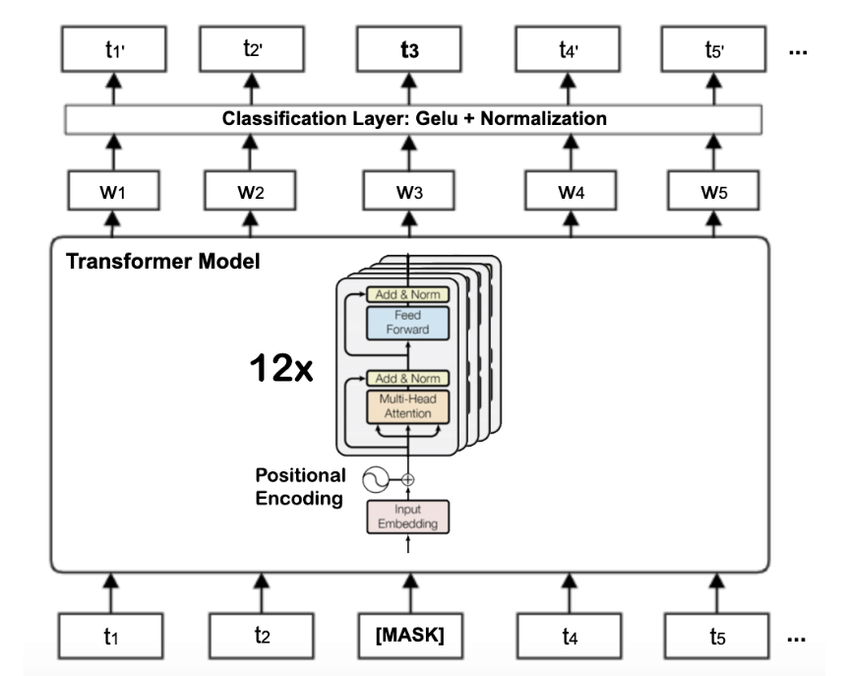
\includegraphics[width=1\textwidth]{images/Chapter1/The-Transformer-based-BERT-base-architecture-with-twelve-encoder-blocks.png} 
	\caption{The Transformer based BERT base architecture with twelve encoder blocks.} 
	\label{fig:Transformer-based-BERT-base-architecture} 
	\medskip
	\small
	(Image taken from \citet{khalid2021rubert}, license CC BY 4.0)
\end{figure}

%During training, the 
%Training objective function, cross-entropy loss:
% "During training, the probability assigned to the correct word is used to calculate the cross-entropy loss for each item in the sequence. As with RNNs, the loss for a training sequence is the average cross-entropy loss over the entire sequence." (Jurasfky 3rd ed. ch.9)(figure 9.21)

%"Attention(23) dynamically assigns a weight to every pair of words in the sequence, indicating how much the model should “pay attention to” the first word when computing the representation of the second one."  \citep{manning2020emergent}
% "Transformers use multiple attention heads in parallel, where  each  head  can  potentially  capture  a  completely  different word–word relation. "
%"Transformers aggregate the information from each head to produce a single output vector representation for each word in the sequence." \citep{manning2020emergent}


Transformer blocks, unlike recurrent neural networks (RNNs), have the computational advantage of not being recurrent, and therefore are highly parallelizable, faster to compute, and scale in a way that RNNs cannot \citep{lau2020furiously}. Transformer based language models contain several millions of trainable parameters. A common baseline model for BERT is composed of 110 million parameters spread over 12 layers of transformer blocks (\autoref{fig:Transformer-based-BERT-base-architecture}). 

They typically require massive amount of data (in the order of at least hundreds of million tokens) and computation time to achieve state of the art performance in natural language processing tasks, and are therefore very expensive to train from scratch, although they can outperform the previous generation of neural language models when properly optimized \citep{manning2020emergent}. 

%"It contains many millions of trainable parameters in  a  number  of  layers,  typically  requiring  massive  amounts  of data  and  computation  to  train.  This  makes  Transformers  difficult  to  train,  but  also  highly  expressive  models  that  can  out-perform  other  contemporary  neural  networks  when  properly optimized" \citep{manning2020emergent}

%"The Transformer architecture (Vaswani et al., 2017) replaces RNN cells with self-attention and point-wise fully connected layers, which are highly parallelizable and thus cheaper to compute."

%transformer blocks "Each provides a multi-headed self-attention unit over all input words, allowing it to capture multiple dependencies between words, while avoiding the need for recurrence. With no need to process a sentence in sequence, the model parallelizes more efficiently, and scales in a way that RNNs cannot" \citep{lau2020furiously}

%\subsection{Transformers and the Attention Mechanism}

%Transformers  are "a neural network architecture,  without  any  recurrent  connections  (22),  which  takes  a sequence  of  words  (or  other  symbols)  as  input  and  produces a contextualized vector representation of each word as its out-put (Fig. 3)."  \citep{manning2020emergent}


%"The key mechanism by which Transformers contextualize representations  is  multi-headed  attention  (see  Fig.  5)."  \citep{manning2020emergent} 
%"attention is a kind of \textbf{generalized dot product}" % (Manning Lecture) https://www.youtube.com/watch?v=aKO1Yok6e4Q&list=PLGJm1x3XQeK0gmqfRkP-VmrEf4UYx5IDW&index=4
%which models all pairwise interactions between words.


% "We provide more mathematical detail below" \citep{manning2020emergent}

%\begin{figure}[H]
%	\centering
%	\includegraphics[width=1\textwidth]{images/Chapter1/attention-manning-pnas.png} 
%	\caption{Overview of the attention mechanism, taken from \citet{manning2020emergent}.} 
%	\label{fig:manning_attention} 
%	\medskip
%	\small
%	(TODO: request permission, pnas licence is CC ND)
%\end{figure}



% a non-recurrent architecture, called the Transformer \citep{vaswani2017attention} 
%The lack of recurrence in the transformers architecture "enables greater within-training-example parallelization, at the cost of quadratic complexity in the input sequence length" \citep{liu2018generating} 

% Jurasfy book (draft new 3rd edition), ch.10 .. \citep[ch.9-10]{jurafsky2021speech} 


% multi-head self-attention of the Transformer

% to reduce memory usage, limiting the dot products between Q and K

% "projecting the tokens into the query, key, and value embeddings"

% decoder-only vs encoder-decoder
% what is an attention head? See "explorable transformers" 

% explorable Bert (online javascript demo): \href{https://huggingface.co/exbert/?model=gpt2&modelKind=bidirectional&sentence=The%20girl%20ran%20to%20a%20local%20pub%20to%20escape%20the%20din%20of%20her%20city.&layer=0&heads=..0,1,2,3,4,5,6,7,8,9,10,11&threshold=0.7&tokenInd=null&tokenSide=null&maskInds=..&hideClsSep=true}{exbert}

% possible TODOs: 
% -give detailed description of each layer dimensions (eg vocab x ..) 
% -compare bert and gpt architecture
% -explain output of gpt and bert

% save the checkpoints of gpt and bert with pythorch inspect the layers

% is dot product in attention a form of linear basis expansion?
% (from machine learning course lectures: name of "augmenting" the input ..)(..appropriate name for semantic info addition?)(LBE, linear basis expansion)(..equivalent to semantic augmentation of the input?)

% schema of the self-attention mechanism (multipling on prev inputs)

% (horizontal vs vertical attention?)

% criticism of attention mechanism (refs)
% alternative attention mechanism
% attention mechanism more efficient for NLP
% auto pruning of attention heads?



% query, key, value




% a  self-supervisedlearning approach. In self-supervised learning, a system is given no  explicit  labeling  of  raw  data,  but  it  is  able  to  construct  its own supervised learning problems by choosing to interpret someof  the  data  as  a  “label”  to  be  predicted \citep{manning2020emergent}

% ?TODO: chapter on ..state of the art / baselines transformer based langugage models ..

% section on overview of NN language models, DL language models, transformers based language models


% The  canonical  case for  human  language  is  the  language-modeling  task  of  trying to  predict  the  next  word  in  an  utterance  based  on  the  tempo-rally preceding words (Fig. 2). Variant tasks include the maskedlanguage-modeling  task  of  predicting  a  masked  word  in  a  text[a.k.a.  the  cloze  task  (11)]  and  predicting  the  words  likely  tooccur  around  a  given  word  (12,  13).  Autoencoders  (14)  canalso be thought of as self-supervised learning systems. Since noexplicit labeling of the data is required, self-supervised learningis  a  type  of  unsupervised  learning,  but  the  approach  of  self-generating supervised learning objectives differentiates it fromother unsupervised learning techniques such as clustering \citep{manning2020emergent}
% (that unsupervised models could not develop interesting knowledge of language) this  has  been  the  dominant  perspective  in  linguistics, where language models have long been seen as inadequateand having no scientific interest, even when their usefulness inpractical engineering applications is grudgingly accepted (15, 16). \citep{manning2020emergent}


\chapter{A Brief Introduction to Island Effects}\label{sec:islands_intro}

%"filler–gap dependencies are subject to numerous complex island constraints:  \citet{ross1967constraints} identified five syntactic positions in which gaps are illicit, dubbing them syntactic islands." \citep{wilcox2018rnn} \\
% "Even though the filler–gap dependency is flexible and potentially unbounded, it is not entirely unconstrained.

% Examples: (..) \\

% psycholinguistic studies (Sprouse)

An \textit{island effect} is the phenomenon of a sentence becoming ungrammatical or unacceptable when there is a long-distance “filler-gap” dependency which crosses the boundaries of certain constructs (as in (\ref{whether_island_1})), which have been metaphorically called syntactic \textit{islands} \citep{ross1967constraints, sprouse2013experimental}.

In psycholinguistic terminology (since \citep{fodor1978parsing}) a filler–gap dependency is the relationship between the antecedent or “filler” (e.g. a complementizer like “\textit{what}” or “\textit{who}” in English, or “\textit{cosa}” or “\textit{chi}” in Italian) and the canonical position (often called “gap”, as a postulated empty position or element with no surface manifestation) of the predicate argument % check if only predicates, or any other constituent, like nouns, that the filler/"argument"/modifier modifies
that it replaces \citep{pearl2013syntactic, wilcox2018rnn, hawkins1999processing}. % the gap can be also referred to as trace or empty category \citep{jurafsky2021speech}
Other terms to refer to filler–gap or long-distance dependencies are syntactic movement or \textit{extraction}\footnote{The use of the term \textit{extraction}, to refer to filler-gap dependencies, evokes the idea of movement formulated in transformational grammars, within the generative linguistic paradigm, as if the filler is moved or extracted from the canonical argument position \citep{sprouse2013experimental}. } \citep{jurafsky2021speech}.

Consider the following examples (taken from \citet{sprouse2016experimental}), in which (\ref{no_filler_gap_1}) is a plain sentence with no “extraction”, and (\ref{filler_gap_1}) contains a filler-gap dependency (the gaps are marked with underscores, and the fillers in bold) :

%\begin{exe}
%	\ex\label{here}
%		\begin{xlist}
%			\ex{Susan thinks that John bought the book.} \label{sub1}
%			\ex{What does Susan think that John bought \_?} \label{sub2}
%			\ex[*]{What does Susan wonder [whether John bought \_]?} \label{sub3}
%		\end{xlist}
%\end{exe}

\begin{exe}
	\ex{Susan thinks that John bought the book.} \label{no_filler_gap_1}
	\ex{\textbf{What} does Susan think that John bought \textbf{\_}?} \label{filler_gap_1}
\end{exe}



% ? todo? separate section for the examples in italian?
% mention here: "(we will discuss equivalent examples for Italian in section ..)"

% names common to English and Italian: Andrea, Lara, ..

% % todo: add an example in italian of a filler-gap dependency
% In the (\subref{sub2}) examples. In the (\subref{sub}) examples.
%\begin{exe}
%	\ex
%	\begin{xlist}
	%		\ex Chi pensa che io abbia riscosso il pagamento?
	%		\ex ..
	%	\end{xlist}
%\end{exe}

%\begin{exe}
%	\ex[*]{Example this ungrammatical is.}
%	\ex[??]{This example questionable is.}		
%\end{exe}
%

% other types of dependencies, different from wh-dependencies (examples inline with parentheses)
% todo: mention here that there are other types of dependencies possible other than wh-dependencies.
% It should be noted here that although island effects are most commonly ..
%"Though island effects are typically exemplified by wh-dependencies, it should be noted that island effects arise with several different types of long-distance dependencies in human languages, such as relative-clause formation (3), topicalization (4), and adjective-though constructions (5):" \citep{pearl2013syntactic}
% (FILLER-GAP DEPENDENCIES, among which WH-questions and relative clauses)
% "we focus here on a single type of long-distance dependency (WH-dependencies in English)" \citep{sprouse2012test}
% other dependencies other than wh-dependencies
%"Though island effects are typically exemplified by wh-dependencies, as in (2), the same effects crucially arise with several different types of long-distance dependencies in human languages: for instance rc-dependencies (3), dependencies between the topicalized preposed constituent and the lower gap (4), and dependencies between the preposed adjective and the lower gap in adjective-though constructions (5). " \citep{sprouse2016experimental}

The dependency in (\ref{filler_gap_1}) is called a wh-interrogative clause dependency (wh-dependency, in short) because the filler is an interrogative wh-word\footnote{More generally, it can be a simple wh-phrase, like "\textit{who}" or "\textit{what}", or a complex wh-phrase, like "\textit{which book}."}. There are however other types of filler-gap dependencies that are blocked by syntactic islands, like relative clause dependencies (rc-dependencies, in short)\footnote{In rc-dependencies, the filler can be either a relative pronoun or a head noun, and it introduces a headed relative clause that hosts the gap, as in the example (from \citet{sprouse2016experimental}) “\textit{I like \textbf{the car} that you think [that John bought \_].}”}. Island effects have been shown to display different patterns of variations with different dependency types, but in the present work we'll focus only on wh-dependencies.



In (\ref{no_filler_gap_1}) the argument \textit{the book} is adjacent to the predicate that selects it (\textit{bought}), while in (\ref{filler_gap_1}) the wh-word \textit{What} is not. Because of this, syntacticians sometimes call wh-dependencies as in (\ref{filler_gap_1}) \textit{long-distance} dependencies, distinguishing them from \textit{short-distance} dependencies as in (\ref{no_filler_gap_1}) where the two constituents in the dependency relationship are adjacent or nearly adjacent to each other \citep{pearl2013syntactic}. 


The distance between the filler and the gap can be made arbitrarily long (as long as human working memory capacity permits), unless a syntactic island intervenes, as in the following examples (taken from \citet{sprouse2013experimental})\footnote{In the examples we use the following notation conventions: the asterisks indicate unacceptable sentences, as it is common in linguistic literature. The syntactic islands constructs, and occasionally other clauses, are marked within square brackets, but this is for explanatory purposes only, they are not part of the sentences given as input to the language models. The gaps are marked with underscores, again for explanatory purposes only.}:
% (we will discuss the respective island effect examples in Italian in \autoref{sec:island_effects_in_italian}):

\begin{exe}
	\ex{What does Susan think that Lily said that Sarah heard that John bought \_?}\label{very_long_distance_1} 
	\ex{\textsc{Whether island:} \\ *What does Susan wonder [whether John bought \_]?} \label{whether_island_1}
\end{exe}

It is worth mentioning here that island effects have been found to decrease with repeated exposure, that is, an individual repeatedly exposed to an island structure such as the one in (\ref{whether_island_1}), will find the resulting sentences acceptable, or less unacceptable \citep{chaves2014subject}.

Island effects are usually named after the type of syntactic structure that creates them \citep{sprouse2013experimental}. The sentence in (\ref{whether_island_1}) exemplifies an extraction from a wh-island, specifically of the whether-island sub-type, that is from an embedded clause headed with the complementizer “whether” \citep{wilcox2018rnn}. Whether islands are among the most easily intelligible types of islands for learners \citep{pearl2013syntactic}, along with Adjunct islands (\ref{adjunct_island_1}), Complex Noun Phrase islands (\ref{complex_np_island_1}) and Subject islands (\ref{subject_island_1}), which are the four types on which we'll focus in the present thesis. The following examples are taken from \citet{sprouse2016experimental}:

\begin{exe}
	\ex{\textsc{Adjunct island} \\ *What does Susan worry [if John buys \_]?} \label{adjunct_island_1}	
	\ex{\textsc{Complex NP Island} \\ *What did Susan make [the claim that John bought \_]?}\label{complex_np_island_1} 
	\ex{\textsc{Subject island} \\ *What did Susan think that [the speech about \_] interrupted the TV show?}\label{subject_island_1}
\end{exe}

In the adjunct island example above (\ref{adjunct_island_1}), there is the extraction of a constituent (the direct object) from an embedded sentential adjunct clause (an adjunct clause is an optional clause which can be omitted without affecting the grammaticality of the main clause \citep{downing2002university}). 

A complex noun phrase is a phrase headed by a noun (“the claim” in (\ref{complex_np_island_1})) with a modifier that is another phrase (“that John bought”). In (\ref{complex_np_island_1}), there is an extraction of a direct object argument (the thing that is bought by John) from the subordinate complex noun phrase (“[the claim that John bought \_”).

In (\ref{subject_island_1}), there is an extraction from a propositional phrase (“about \_”) that modifies a noun phrase (“[the speech about \_ ]”) that occurs in the subject position (for the verb “interrupted”) of a subordinate clause \citep{wilcox2018rnn, sprouse2016experimental}.

% "1 In the syntactic literature it is common to use the label “complex NP island effects” to refer both to extraction from the clausal complement of a noun, as in (2b), and from a relative clause as in (2e). In this paper we use a stricter terminology and use “complex NP island” to refer only to the clausal complement of a noun. See Cecchetto and Donati (2015) for a nonstandard view of this construction."  \citep{sprouse2016experimental}

% todo: variations of these phenomena, differences smong them, mentioned by Sprouse
% TODO: add equivalent examples also for italian
% for wh-dependencies, and subject islands in italian, is there a restriction to PPs only, or also subjects and direct objects?



%\section{Wh-islands and whether Islands}\label{sec:wh_islands}
% todo: subsections for each of the four island types: e.g. 

% for wh/wheter islands ..a few word on differences, variations, examples for the different studies (sprouse, hu, wilcox, blimp, rizzi); examples, variations, differences in italian

%Wh-Island Constraint definition: 
%"A gap cannot appear inside doubly nested clauses headed by wh-complementizers. This phenomenon is called the Wh-Island Constraint (WHC). "  \citep{wilcox2018rnn}

%Adjunct Island Constraint
%"We used three different prepositions to construct temporal adjuncts: ‘while’, ‘after’ and ‘before’." \citep{wilcox2018rnn}


%\section{Adjunct islands}\label{sec:adjunct_islands}
% for adjuncts, with example of conditional and temporan adjuncts; the fact that they were first studied in 1982

%\section{Complex NP islands}\label{sec:complex_np_islands}
% same for complex np and subject islands: examples from the different studies (sprouse, hu, wilcox, blimp, rizzi) showing variations, differences in italia (italian examples when possible)
% cite also examples from the paper on norwegian and the one by .. and Zamparelli

%\section{Subject islands}\label{sec:subject_islands}



\section{The importance of island effects in linguistics}


% mention a lot of research in linguistics on island effects

The linguistic research on island effects has received prominence for their role in arguments on the innate nature of the language faculty. A staple of proponents of the linguistic paradigm known as \textit{generative linguistics}, which since its first formulation by \citet{chomsky1957syntactic} has been the hegemonic linguistics paradigm for decades, is the Universal Grammar hypothesis (UG) \citep{chomsky1965aspects}, according to which the language faculty is innate, and the acquisition of language is made possible by the presence of innate linguistic constraints or biases in the human brain \citep{dkabrowska2015exactly}. According to the most common definitions, the "universal grammar" present in the brain would consist of an innate “system of categories, mechanisms and constraints shared by all human languages”,  which includes "principles", general constraints to which all human language grammars must abide, and "parameters", which are the possible variations in grammatical features between languages \citep{dkabrowska2015exactly}.

One of the main and most influential argument in support of the Universal Grammar hypothesis, has been the Argument from the Poverty of the Stimulus (APS), according to which  linguistic knowledge possessed by children cannot be acquired exclusively from the input which is available to them, therefore they must possess some innate knowledge of it \citep{pullum2002empirical}. 

%"the claim that children have linguistic knowledge which could not have been acquired from the input which is available to them:"  \citep{dkabrowska2015exactly}
%"The argument type in question turns on the claim that during the language acquisition process, children often come to know things about the language they are acquiring despite not having access to the crucial evidence that shows those things to be true of the language."
% an argument in favor of UG, is the poverty of the stimulous argument
% the claim that a grammatical approach to island effects necessitates innate linguistic constraints .. innate linguistic biases (i.e., UG)
% innate knowledge, able to learn non-trivial ..
%"The influential argument from the poverty of the stimulus (APS) ..  has been subject to much criticism (Pullum and Scholz, 2002)"  Geoffrey K. Pullum and Barbara C. Scholz. 2002. Empirical assessment of stimulus poverty arguments. The Linguistic Review, 18(1-2):9–50.


Island constraints have been central in proposals for the innate presence of complex linguistic biases in the human brain, for the Argument from the Poverty of the Stimulus, and in the debates on generative UG-based syntactic theories \citep{pearl2013syntactic}. 
% "Because of their complexity and ubiquity, these dependencies have figured prominently in arguments that natural language would be unlearnable by children without a great deal of innate knowledge (Phillips, 2013) (cf. Pearl and Sprouse, 2013; Ellefson and Christiansen, 2000)" \citep{wilcox2018rnn} 
This is due to the fact that island effects are a complex phenomenon, rare or non-existent in child-directed speech (and of relative infrequency even in adult-directed speech), which therefore "raise difficult questions about how children could use their limited input to arrive at a grammar that includes long-distance dependencies that are nonetheless constrained by specific structural configurations. In this way, island effects provide a classic motivation for theories that assume domain-specific constraints on language acquisition (i.e. universal grammar)" \citep{sprouse2012test}.
% "Furthermore, given the relative infrequency of multiclausal WH-dependencies even in adult-directed speech," \citep{sprouse2012test}.

%“no negative evidence”
%"Between the centrality of syntactic island effects as a topic of research in (generative syntactic theory and the reliance on a UG-based mechanism for their acquisition, it seems clear that syntactic island effects are an ideal case study in the role of innate, domain-specific learning biases in language acquisition."  \citep{pearl2013syntactic}

For this reason, since their discovery by \citet{ross1967constraints}, they have been heavily investigated and been a subject of debate in the linguistic and psycholinguistic literature, with hundreds of articles in dozens of languages devoted to their investigation \citep{sprouse2013experimental, pearl2013syntactic}.
%importance of island effects in linguistics
%Since when "island effects were first investigated \citep{chomsky1965aspects, ross1967constraints} there have been literally hundreds of articles in dozens of languages devoted to the investigation of island effects, resulting in various proposals regarding the nature of island constraints and the cross-linguistic variability of island effects". 

One of the main arguments against the existence of proper island "constraints" that render a sentence ungrammatical when violated, is that such ungrammaticality or unacceptability could arise instead discourse-structural factors or simply from the increased \textit{processing difficulty} due to the sum of other factors present in alleged "island violations", like the fact of having a long-distance dependency combined with more marginal syntactic constructs \citep{sprouse2013experimental, wilcox2018rnn, ambridge2008island, hofmeister2010cognitive}. 
% "open question whether these “island constraints” are true grammatical constraints, or whether they are effects of processing difficulty or discourse-structural factors (Ambridge and Goldberg, 2008; Hofmeister and Sag, 2010; Sprouse and Hornstein, 2014)" \citep{wilcox2018rnn} 

% As \citet{sprouse2013experimental} explain it: 
%"As an acceptability-based phenomenon, the source of island effects has long been a topic of debate within the linguistic and psycholinguistic literature."  \citep{sprouse2013experimental}
%\begin{displayquote}
%"The problem lies in the fact that acceptability judgments are a behavioral response that is the result of successful sentence processing (Chomsky 1965, Schutze 1996, Sprouse and Almeida 2013), and as such could be influenced %¨ 
%by any of the cognitive systems that are implicated in successful sentence processing, from the multiple mental representations that can be used to characterize a sentence (e.g., phonological, morphological, syntactic, semantic, pragmatic), to the different components of the parsing system that must be deployed during normal sentence comprehension (e.g., structure-building operations, ambiguity resolution heuristics, working memory systems)." 
%\end{displayquote}
%"In short, this is the classic problem of cognitive science (mapping observable behavioral responses to unobservable cognitive constructs), exacerbated by the complexity and multi-level nature of human language." "The primary empirical goal of this volume is to bring the techniques of experimental syntax (broadly construed) to bear on this particular instantiation of the cognitive science problem, and move the field one step closer to identifying the source of island effects." \citep{sprouse2013experimental}

% theories of island effects
%"there is substantial variability within the class of grammatical approaches. There are syntactic approaches to island effects, which posit syntactic constraints known as island constraints on the formation of WH-dependencies, such as Ross’s classic COMPLEX NP CONSTRAINT (Ross 1967), Chomsky’s SUBJACENCY CONDITION (Chomsky 1973, 1986), and Huang’s CONDITION ON EXTRACTION DOMAINS (Huang 1982). There are also semantic approaches to island effects,  for example, the algebraic semantics approach to weak islands by Szabolcsi and Zwarts (1993), the event structure account of adjunct islands by Truswell (2007), and the presupposition failure account of negative islands, factive islands, and others by Abrusán (2011). Some other grammatical approaches are more pragmatic in nature (ErteschikShir 1973, Kuno 1976, 1987, Kuno \& Takami 1993, Goldberg 2007)."  \citep{sprouse2012test}
% "Furthermore, the predominant analysis of syntactic island effects in generative syntactic theory is well known to rely on innate, domain-specific learning biases. For example, in the Government and Binding framework of the 1980s, syntacticians proposed a syntactic constraint called the Subjacency Condition, which basically holds that the dependency between a displaced element (e.g., a vWi-word) and the gap position cannot cross two or more bounding nodes (Chomsky 1973; Huang 1982; Lasnik \& Saito 1984, and many others)." \citep{pearl2013syntactic}
% "The definition of bounding nodes can vary from language to language in order to account for the various patterns of island effects that have been observed cross-linguistically. For example, the bounding nodes in English are argued to be NP (Noun Phrase) and IP (Inflection Phrase) (Chomsky 1973), while the bounding nodes in Italian and Spanish are argued to be NP and CP (Complementizer Phrase) (Rizzi 1982; Torrego 1984). Crucially, this framework assumes that the Subjacency Condition itself is part of UG, as are the possible options for bounding nodes (NP, IP, or CP). The language learner then simply needs to determine which bounding nodes are relevant for her specific language in order to learn syntactic island constraints. Although recent evolutions of syntactic theory have terminologically abandoned Subjacency and bounding nodes, it has been argued that modern incarnations of syntactic constraints (such as phase impenetrability) are essentially formal variants of the original Subjacency analysis (Boeckx \& Grohmann 2007)." \citep{pearl2013syntactic}

%"Though most of this literature is beyond the scope of the present article, it does serve to underscore\textbf{ the central role that syntactic island effects have played in the development of (generative) syntactic theory}" \citep{pearl2013syntactic}


%"island effects provide a classic motivation for theories that assume domain-specific constraints on language acquisition (i.e. universal grammar)." \citep{sprouse2012test}
%"In chapter 5, Pearl and Sprouse address one of the motivations for the debate between grammatical and reductionist accounts: the claim that a grammatical approach to island effects necessitates innate linguistic constraints (i.e., Universal Grammar)." 

To address poverty of the stimulus arguments regarding island effects, a psycholinguistic study by Pearl and Sprouse \citep{sprouse2013experimental} implemented  a computational model able to learn island constraints corpus of child-directed speech, without any prior linguistic bias (like a Universal Grammar). % "Contrary to this claim, Pearl and Sprouse propose (and implement) a computational model that can learn island effects as a type of grammatical constraint from a corpus of child-directed speech without resorting to innate linguistic biases (i.e., UG)." \citep{sprouse2013experimental}
Modern deep neural language models have also began to be used as an argument that a system without any prior linguistic learning biases can learn non-trivial syntactic phenomena and other hierarchical structures \citep{linzen2018can}. For instance \citet{gulordava2018colorless} wrote: "We tentatively conclude that LM trained RNNs can construct abstract grammatical representations of their input. This, in turn, suggests that the input itself contains enough information to trigger some form of syntactic learning in a system, such as an RNN, that does not contain an explicit prior bias in favor of syntactic structures". And \citep{warstadt2020blimp}: "By evaluating whether self-supervised learners like LMs acquire human-like grammatical acuity in a particular domain, we gather indirect evidence as to whether this phenomenon is a necessary component of humans’ innate knowledge".
% "Of particular interest, both for linguistics and for building better models, is whether deep models’ representations encode syntax (Linzen, 2018)" \citep{hewitt2019structural}.

%"Recent work has analyzed model behavior to determine if a model understands hierarchy and other linguistic phenomena (Linzen, 2018; Gulordava et al., 2018; Kuncoro et al., 2018; Linzen and Leonard, 2018; van Schijndel and Linzen, 2018; Tang et al., 	2018; Futrell et al., 2018)." \citep{hewitt2019structural}

%"Furthermore, the extent to which humans resemble data-driven learners like language models is debated in linguistics and cognitive science (see e.g., Chomsky, 1965; Reali and Christiansen, 2005). In some domains, we may require the aid of innate knowledge to acquire phenomenon-specific knowledge resembling that tested in BLiMP."  warstadt 2020 blimp


%mention phenomena that ameliorate the acceptabily of island effects: parasitic gaps , resumptive pronouns


%\subsection{Language acquisition theories and Syntactic islands}

% intro with discovery by Ross, and cross linguistic analysis by Rizzi
% (generativist theory assumptions and terminology since then abandoned, some concepts fro islands remained..)

%language acquisition and UG


%"potential problems posed by syntactic island effects for any theory of syntactic acquisition." "previous theories of syntactic island learning" "difficult questions about how the specific biases required by syntactic islands arise in the learner." \citep{pearl2013syntactic}
%"the syntactic theories of UG proponents." \citep{pearl2013syntactic}

%"to truly test the UG hypothesis, and in order for the resulting acquisition models to have a real impact on existing syntactic theories (Chomsky 1965), we need to choose a set of syntactic phenomena that are central to (UG-based) syntactic theories." \citep{pearl2013syntactic}



%"while the methodology for testing learning biases is relatively clear, the data required to actually perform those tests are still relatively scarce"   \citep{pearl2013syntactic}


% "In chapter 5, Pearl and Sprouse address one of the motivations for the debate between grammatical and reductionist accounts: the claim that a grammatical approach to island effects necessitates innate linguistic constraints (i.e., Universal Grammar). Contrary to this claim, Pearl and Sprouse propose (and implement) a computational model that can learn island effects as a type of grammatical constraint from a corpus of child-directed speech without resorting to innate linguistic biases (i.e., UG)." \citep{sprouse2013experimental}


\section{Cross-linguistic variation in island effects}

Cross-linguistic variations have been observed for island effects, since the first study on island effects in Italian by \citet{rizzi1982violations}.  % 
While English shows at least eight different types of island effects (whether islands, complex NP islands, subject islands, adjunct islands, relative-clause islands, sentential subject islands, coordinate structure constraint violations, and left branch extraction violations), Scandinavian languages (Swedish, Norwegian,
Danish, and Icelandic), show almost no island effects\footnote{\citet{sprouse2013experimental} report that "Swedish is not bereft of apparent island effects. Rather it does not display island effects in all contexts where they are theoretically expected to appear (and as they do appear in English). For example, there are some unacceptable instances of extracting out of complex noun phrases, but others seem perfectly fine."} \citep{pearl2013syntactic}. Here are examples of the above mentioned eight types of syntactic islands in English, taken from \citet{sprouse2013experimental}:

\begin{example}
	Island effects in English
	\renewcommand{\labelenumi}{\alph{enumi}.}
	\begin{enumerate}
		\item \textsc{whether island:} \\
		*What do you wonder [ whether John bought \_]?
		\item \textsc{complex NP island:} \\
		*What did you make [ the claim that John bought \_]?
		\item \textsc{subject island:} \\
		*What do you think [ the speech about \_] interrupted the TV show?
		\item \textsc{adjunct island:} \\	
		*What do you worry [ if John buys \_]?
		\item \textsc{relative-clause island:} \\	
		*What did you meet [ the scientist who invented \_]?
		\item \textsc{sentential subject island:} \\	
		*What did [ that John wrote \_] offend the editor?
		\item \textsc{coordinate structure constraint violation:} \\	
		*What did John buy [ a shirt and \_]?
		\item \textsc{left branch extraction violation:} \\	
		*Which did John borrow [ \_ book]?	
	\end{enumerate}
	\label{en_islands}
\end{example}

Most island effects are present in Romance languages, with some exceptions, as some types of syntactic islands have effect in certain types of sentences, but not in others. This is the case of subject islands, which are not present in Italian, Spanish and Portuguese, while they are present in French \citep{pearl2013syntactic}. In a psycholinguistic study, \citet{sprouse2016experimental} found evidence that subject islands with relative clause dependencies are not present in Italian. 
% As noted by \citet{sprouse2013experimental}, this kind of variability "has proven challenging for approaches to island effects that postulate a source that is outside of the grammar (e.g., components of the sentence processing system), as grammatical theories have traditionally been the sole locus of cross-linguistic variation"
% "To the extent that Table 1.1 is accurate, the cross-linguistic variation it reports raises some very interesting questions for theories of island effects. For example, it has proven relatively difficult to characterize precisely the variability indicated by question marks; that is, island effects in certain languages that appear arise for some sentences, but not others. Furthermore, the mere existence of variability has proven challenging for approaches to island effects that postulate a source that is outside of the grammar (e.g., components of the sentence processing system), as grammatical theories have traditionally been the sole locus of cross-linguistic variation." \citep{sprouse2013experimental}

There is also a substantial varying degree of acceptability between the different types of islands. For instance, wh-islands are generally among the strongest sources of sentence acceptability, while violations of complex NP islands with rc-dependencies tend to be more acceptabile \citep{pearl2013syntactic}. Because of this, it has been proposed in the literature a distinction between strong and weak islands \citep{sprouse2016experimental, szabolcsi2006strong}.
% "Furthermore, it has long been noted that the degrees of unacceptability substantially differ across the various islands. For example, violations of the WH-island condition are generally less unacceptable than violations of the relative clause version of the Complex Noun Phrase Constraint"  \citet{sprouse2013experimental}
% "For discussion of these matters see chapter 3 (Hofmeister et al.), chapter 4 (Phillips), chapter 11 (Kush et al.), chapter 12 (Jurka), chapter 13 (Polinsky et al.)." \citep{sprouse2013experimental}
% "\textbf{distinction between strong and weak islands} in the literature (for a review see Szabolcsi 2006)" \citep{sprouse2016experimental, szabolcsi2006strong}
% so from weakest to strongest ("more prototypical) islands, the order should be:
% whether, complex np, subject, adjunct (swap the last 2?)
Furthermore, the acceptability of island violations also varies from speakers to speaker within the same language, with some speakers being more sensitive than others to island effects \citep{sprouse2013experimental}.

%Table 1.1 in \citet{sprouse2013experimental}
%"Table 1.1 presents nine languages that are known to employ wh-movement in questions, and five of the most studied island effects: WH-islands (3a), Complex Noun Phrase islands (3b), Subject islands (3c), Adjunct islands (3d), and Relative Clause islands (3e). The diacritics indicate whether the specified language demonstrates that particular island effect: asterisks indicate that the island effect arises in that language, dashes indicate that the island effect does not arise in that language, and question marks indicate that the island effect arises for some sentence types, but not others." \citep{sprouse2013experimental}
%"We should note that Table 1.1 idealizes the empirical results to a considerable extent. There has been considerable work on these cross-linguistic differences and the differences noted here are not nearly as categorical as displayed. For example, many English speakers treat the wh-island violations discussed in Rizzi 1982b as acceptable (c.f. Grimshaw 1986)"  \citep{sprouse2013experimental}
%
% % is there a linguistic continuum in the cross-linguistic variation of island effects, from more prototipical to less ones?


% "Whereas the first pattern in Table 1.1 primarily concerns Romance languages, the second pattern concerns Scandinavian languages (Swedish, Norwegian, Danish, and Icelandic). As first observed by Engdahl (1980) for Swedish, Scandinavian languages do not demonstrate any of these five island effects.6" \citep{sprouse2013experimental}
%"In either case, the existence of apparently island-less languages such as modern Scandinavian languages raises interesting challenges for any comprehensive theory of island effects." \citep{sprouse2013experimental}


% " the argument/adjunct distinction that has been observed in so-called wh-in-situ languages such as Chinese (Huang 1982a), Japanese (Lasnik and Saito 1984), and Sinhala (Hagstrom 1998). In wh-in-situ languages, question formation does not involve displacement of the wh-word: the wh-word appears in the same position that the questioned constituent would appear in a declarative sentence (i.e., the gap-position in wh-movement languages)." \citep{sprouse2013experimental}



% "2.3 Resumptive pronouns"

% "Although most of the languages discussed so far exclusively employ gap positions as the foot of long-distance dependencies, about half of the world’s languages appear to allow a second option: resumptive pronouns. Resumptive" "pronouns are lexically indistinguishable from regular pronouns, but appear in the position that under other circumstances would be the gap position of a long-distance dependency (McCloskey 2006). When it comes to the interaction of resumptive pronouns and island effects, McCloskey (2006) identifies three types of languages." \citep{sprouse2013experimental}

% "The relevance of resumptive pronouns in free-variation languages for the theory of island effects rests in their dual nature (which McCloskey (2006) describes as Janus-like): whereas true gaps are canonically associated with long-distance dependencies that are sensitive to island effects, and true pronouns are canonically associated with a type of long-distance dependency that is not sensitive to island effects (i.e., binding relations), resumptive pronouns fall in between by allowing non-binding long-distance dependencies to cross island structures.8" "8It should be noted that the relevance of resumptive pronouns to island effects was first observed by Ross (1967). He noted that resumptive pronouns obviate island effects when present. As he also assumed that they are related to their antecedents via movement, he concluded that movement per se could not be island-sensitive. The approach discussed by McCloskey (2006) inverts this logic: binding is different from movement and the latter is island-sensitive while the former is not. Importantly both point to a conclusion of current interest: that overt gaps make a difference even if the dependency looks similar. The problem is not the dependency but how it is formed." \citep{sprouse2013experimental}

% "Type 3: Intrusive pronoun languages
% In the third type of language, exemplified by English, resumptive pronouns are not a grammatical option (14a versus 14b). However, native speakers tend to spontaneously produce resumptive pronouns inside of island structures as in (15a), apparently in an attempt to avoid the island effects that arise when gaps appear inside island structures (15b).10 (14) a. That’s the donkey that __ is from Brazil. b. *That’s the donkey that it is from Brazil. (15) a. *That’s the donkey that I don’t know where __ is from. b. ?That’s the donkey that I don’t know where it is from. Sells (1984) suggests that the English-type resumptive pronouns be called intrusive pronouns to distinguish them from the resumptive pronouns that appear in languages that allow resumption as a grammatical option. This, of course, raises the question of whether resumption is a unitary phenomenon, or whether there are in fact two, or even three, distinct types of resumptive pronouns in the languages of the world (see McCloskey 2006 for a discussion)."  \citep{sprouse2013experimental}

% "2.4 Parasitic gaps"
% "Parasitic gap constructions are long-distance dependencies in which the displaced element is associated with two gap positions: one gap position occurs in a licit gap location (i.e., not inside an island structure) while the other gap position occurs inside an island structure (Engdahl 1983). Whereas a single gap within an island structure results in unacceptability (16a and 17a), \textbf{the addition of another gap outside of the island structure seems to make the sentence acceptable} (16b and 17b):" \citep{sprouse2013experimental}

% "(16) a. *Which book did you laugh [before reading __]?
% b. Which book did you judge __true [before reading __parasitic]?
% (17) a. *What did [the attempt to repair __] ultimately damage the car?
% b. What did [the attempt to repair __parasitic] ultimately damage __true?"

% "The two gaps in a parasitic gap construction are often described as the true gap, which occurs outside of the island, and the parasitic gap, which occurs inside of the island. The name is a metaphorical reference to the fact that the parasitic gap could not exist without the true gap, much like a parasite cannot exist without a host."


%"The nature of the licensing restrictions on parasitic gaps is an active area of research, and as such a complete review is beyond the scope of this chapter (see Culicover and Postal 2001 for a collection of papers dedicated to parasitic gaps)."  \citep{sprouse2013experimental}
%
%" However, Culicover (2001) lays out several properties that any theory of parasitic gaps must accommodate, and therefore any theory of island effects must accommodate, three of which we will review here." \citep{sprouse2013experimental}

% "Although each of these properties of parasitic gaps receives an impressive amount of empirical support in the syntactic literature, there are also quite a few counterexamples to each property (see Culicover 2001 for a review). Each property (and counterexample) provides both an interesting question that could be addressed with experimental syntax techniques, and an interesting challenge for any comprehensive theory of island effects."  \citep{sprouse2013experimental}

% facts on island effects:
% (i) "The (potentially constrained) variation observed in Romance and Scandinavian languages with respect to types of island effects;" \citep{sprouse2013experimental}
% (iii)) The interaction of resumptive pronouns with island effects in Irish-type, Vata-type, and English-type languages;
% (iv) The existence of parasitic gaps that can (grammatically) appear inside of island structures, as well as the restrictions on their appearance." \citep{sprouse2013experimental}



% note on LM assessment on other phenomena
% Cross-linguistic differences, italian, english "Differences across languages. English was by far the hardest language. We conjecture that this is due to its poorer morphology and higher POS ambiguity, which might not encourage a generic language model to track abstract syntactic configurations." "In languages such as Italian and Russian, which have richer morphology and less ambiguity at the part-of-speech level than English, the LSTMs show much better accuracy and a smaller gap between original and nonce sentences. " Gulordava et al 2018


\section{Island effects in Italian}\label{sec:island_effects_in_italian}

%As an introductory description of island effects, we list here examples of the four types of islands in Italian for which we conducted experiments. We give a fuller description of our test suite in  \autoref{sec:testsuite_design}.


% "For this article, we decided to test syntactic island effects in English and Italian because these two languages have been cited as evidence for cross-linguistic variation in syntactic island effects (e.g., Rizzi 1982)" \citep{sprouse2016experimental}
% "The seminal study on island effects in Italian is by \citep{rizzi1982violations}, who first observed that Italian does not exhibit the same set of island effects as English." \citep{sprouse2016experimental}


%\begin{exe}
%	\ex \gll Tu pensi	che io abbia comprato il libro.\\
%			You	think 	that I have bought the book\\
%	\glt `You think I bought the book'\label{no_filler_gap_1_it}
%\end{exe}

%\begin{exe}
%	\ex{\textsc{Whether island}}
%		\begin{xlist}
	%				\ex\gll *Cosa ti domandi se io abbia comprato \_?\\
	%					What yourself wonder if I have bought \\
	%					\glt `What do you wonder if I bought?'\label{whether_island_1_it}
	%				\ex ..
	%		\end{xlist}
%\end{exe}

% (Some examples taken from \citep{sprouse2016experimental})



%
%"The other examples in (2) demonstrate that most other island types do not involve wh-words or phrases therefore can be investigated in Italian in wh-interrogatives without modification"  \citep{sprouse2016experimental}


Island effects in Italian were first studied by \citet{rizzi1982violations}, which observed some cross-linguistic variation between English and Italian.
%"One fact worth noting is that Rizzi (1982) focused on relative clause formation as opposed to wh-interrogative clause formation in his study of island effects in Italian. This contrasts with most studies of island effects in English, which have tended to focus on wh-interrogatives rather than relative clauses."  \citep{sprouse2016experimental}
While most studies of island effects in English usually focus on syntactic island built with wh-interrogatives, in his study Rizzi focused only on syntactic islands under relative clause dependencies, arguing that it was problematic study them with wh-dependencies because they would require a double wh-word (as in \textit{*Chi ti domandi chi \_ ha incontrato \_?})(\textit{Who do you wonder who met?}), which itself renders a sentence unacceptable, resulting in a confound. 
However, \citet{sprouse2016experimental}, which assessed the same types of islands with wh-dependencies in English and Italian speakers, showed that is possible to circumvent this problem, by studying wh-dependencies with island types that do not require a second wh-word. Specifically, for a direct cross-linguistic comparison, they studied wh-dependencies with whether-islands in English, and \textit{se}-islands ("\textit{if}") in Italian.
% \citet{rizzi1982violations} argued that it was not possible to isolate the effect of wh-islands violations in Italian, because in this language there is a double-wh-prohibition ..

Here are some of the examples of islands with rc-dependencies studied by \citet{rizzi1982violations} (the translations are from \citet{sprouse2016experimental}):

\begin{exe}
	\ex{\textsc{Wh-island} \\ Tuo fratello, a cui mi domando che storie abbiano raccontato \_ \_, era molto preoccupato.\\ "Your brother, who I wonder what stories they told, was really worried."}\\
	\ex{\textsc{Complex NP Island} \\ {*Questo incarico, che non sapevo [la novità che avrebbero affidato \_ a te], ...} \\ "This task, which I didn't know the new that they may have assigned to you..."}\\
	\ex{\textsc{Subject island} \\ Questo autore, di cui so che [il primo libro \_] è stato pubblicato recentemente, ...\\ "This task, which I didn't know the new that they may have assigned to you..."} \\
\end{exe}
%
%\begin{exe}
%	\ex{\textsc{Wh-island}} 
%	\begin{xlist}
	%		\sn\gll Tuo fratello, a cui mi domando che storie abbiano raccontato \_ \_, era molto preoccupato.%\\
	%		\glt "Your brother, who I wonder what stories they told, was really worried."
	%	\end{xlist}
%	\ex{\textsc{Complex NP island}} 
%	\begin{xlist}
	%		\sn\gll{*Questo incarico, che non sapevo [la novità che avrebbero affidato \_ a te], ...}%\\
	%		\glt "This task, which I didn't know the new that they may have assigned to you..."
	%	\end{xlist}
%	\ex{\textsc{Subject island}} 
%	\begin{xlist}
	%		\sn\gll Questo autore, di cui so che [il primo libro \_] è stato pubblicato recentemente, ...%\\
	%		\glt "This author, who I know that the first book was published recently, ..."
	%	\end{xlist}
%\end{exe}

% However, the above four syntactic islands are constructed with wh-dependencies, and these configurations have been shown to produce island effects in both English and Italian \citep{rizzi1982violations, sprouse2016experimental}.
In the present thesis, we focus on assessing island effects under wh-dependencies, which have been shown to produce island effects in both English and Italian \citep{rizzi1982violations, sprouse2016experimental}. The following (\ref{whether_island_1_it}-\ref{subject_island_1_it}) are examples in Italian with wh-dependencies and the four island types administered to language models in our experiments:

\begin{exe}
	\ex{\textsc{Whether island}} 
	\begin{xlist}
		\sn\gll *Cosa ti domandi [se io abbia comprato \_]?\\
		What yourself wonder if I have bought\\
		\glt `What do you wonder if I bought?'\label{whether_island_1_it}
	\end{xlist}
	\ex{\textsc{Adjunct island}} 
	\begin{xlist}
		\sn\gll {*Che cosa} Gianni è partito per Parigi [dopo aver fatto \_]?\\
		What Gianni is left for Paris after having done\\
		\glt `What did Gianni leave for Paris after packing?'\label{adjunct_island_1_it}
	\end{xlist}
	\ex{\textsc{Complex NP Island}} 
	\begin{xlist}
		\sn\gll *Cosa hai fatto [{l’affermazione} che il tuo amico avrebbe mandato \_]?\\
		What have done {the statement} that the your friend have sent\\
		\glt `What did you make the claim that your friend sent?'\label{complex_np_island_1_it}
	\end{xlist}
	\ex{\textsc{Subject Island}} 
	\begin{xlist}
		\sn\gll *Di chi pensi che [la {moto \_]} abbia urtato {l'auto} di Chiara?\\
		of who think that the motorbike have hit {the car} of Chiara\\
		\glt `Who do you think the motorike of hit Chiara's car?'\label{subject_island_1_it}
	\end{xlist}
\end{exe}

In all of the items, the fillers are simple wh-words (e.g. "\textit{cosa}", "\textit{chi}")("\textit{what}", "\textit{who}"), rather than complex wh-phrases ("\textit{che libro}")("\textit{which book}") %(which have also been referred in the literature as D-linked wh-phrases). 
This is because these are the most commonly studied types of wh-dependencies for syntactic islands, and also to match the examples is \citep{sprouse2016experimental} for comparison purposes. The type of wh-words (simple vs complex) is one of the factor that in principle could affect the processing of island effects and therefore their acceptability.

One aspect that influences the difference in sentence structure of syntactic islands in Italian, is the fact that Italian does not allow \textit{preposition stranding as in English}. Preposition stranding is the possibility of having a preposition \textit{stranded} (separated from) its object. For example, in the English sentence \textit{I know \textbf{who} you bought the painting \textbf{from}}, "from" and "who" are stranded. Instead, Italian forces "\textit{pied-piping}" (another metaphorical technical term introduced by \citet{ross1967constraints}, like that of "islands", as mentioned in \autoref{sec:islands_intro}), the fact that the prepositional phrase must be continuous (the wh-word \textit{brings along} the preposition): \textit{So \textbf{da chi} hai comprato il quadro} ("\textit{I know from who you bought the painting}").

%"As we will see in the next section, the variation in island effects between English and Italian involves both interrogative clause formation and related wh-dependencies (2) and headed relative clause formation and related rc-dependencies (3)"  \citep{sprouse2016experimental}



% complex wh-phrases
% teasing apart properties, disentangling confounds:
% "The two dependency types tested in our experiments vary not only by type (wh vs. rc), but also by featural specification of the head of the dependency." 
% "In particular, wh-dependencies are introduced by bare wh-words while rc-dependencies are introduced by a combination of a nominal head followed by a wh-word. This raises the question: Was the variation in island effects observed in our experiments due to the dependency type or due to the featural specification of the heads?8" "To attempt to disentangle these two properties in English, we decided to test wh-dependencies that are introduced by complex wh-phrase in which a wh-word combines with a nominal (e.g., which car) with all four island types." 
% "In principle, complex wh-phrases might behave differently from bare wh-words for two reasons. "
% "First, they are more likely to be D-linked, i.e., their interpretation crucially depends on contextually salient sets of individuals."
% "Second, intervention effects for complex wh-phrases have been observed to be different from intervention effects with bare wh-words, at least in child grammar (see Friedmann et al. 2009). These two properties of complex wh-phrases have led to the use of at least two terms in the literature to refer to these phrases: D-linked wh-phrases, which tends to be used to highlight the D-linking property, and lexically restricted wh-phrases, which tends to be used to highlight the contribution of the noun to Relativized Minimality effects (e.g., Friedmann et al. 2009)." \citep{sprouse2016experimental}

% formulating a prediction (expected results if an hypothesis holds or is rejected) 
% "The overlapping similarities between complex wh-phrases and bare wh-words on one hand, and complex wh-phrases and relative clause heads on the other, make the following predictions. If it is the dependency type that is driving the variation, then wh-dependencies with complex wh-phrases will display the same pattern of island effects as wh-dependencies with bare wh-words; if it is the featural specification that is driving the variation, then wh-dependencies with complex wh-phrases will display the same pattern of island effects as rc-dependencies (regardless of whether it is ultimately D-linking, intervention, or even processing difficulty issues that are underlying the featural specification effect)" \citep{sprouse2016experimental}
% "To test this question we simply changed the bare wh-words in the first four English experiments to complex wh-phrases (the full set of materials is on the first author’s website). We kept all other details of the experiment identical, including the number of participants tested (56 for each of 4 experiments), the method of recruitment (Amazon Mechanical Turk), the details of the surveys (e.g., the order of presentation of items), and the analysis of the results (z-score transformations and linear mixed effects models). "  \citep{sprouse2016experimental}
% "One welcome consequence of this minimal change in experimental materials is that these four experiments serve as both a test of complex wh-dependencies and a replication of the rc-dependency results reported in Sect. 5 (because the rc-dependency materials are unchanged in these new experiments). Given that it was the rc-dependency results that differed from previous reports in the literature, this replication is an important step in establishing the reliability of these results"   \citep{sprouse2016experimental}



%"all of the rc-dependencies in Italian had to be constructed with oblique (PP) argument gaps because Italian restrictive relatives can only be introduced by a relative pronoun when the head of the relative is an oblique argument (subjects and direct objects can only be introduced by the complementizer che ‘that’). This led to a systematic difference between Italian rc-dependencies, which were constructed with oblique argument gaps, and English rc-dependencies, which were constructed with direct object gaps."  \citep{sprouse2016experimental}
%"Italian subject islands involve PP extraction, while English subject islands involve DP extraction" \citep{sprouse2016experimental}
%
%"the lack of preposition stranding in Italian meant that the gap locations of the oblique (PP) arguments were not unambiguously signaled." 
%"For wh-islands, complex NP islands, and adjunct islands, we were able to minimize potential ambiguity through the careful selection of predicates. However, a pilot experiment suggested that this was not possible for subject islands because of the presence of a second NP (the object) that could be modified by the displaced PP."  \citep{sprouse2016experimental}
%"To remedy this, we decided to modify the factorial definition of subject islands slightly. Whereas the factor GAP-POSITION in the canonical factorial definition in (12) varies between MATRIX SUBJECT and EMBEDDED-SUBJECT gap positions, the modified subject island definition varies between EMBEDDED-OBJECT and EMBEDDED-SUBJECT gap positions. This allows us to include a PP adjunct with both the subject and object NP, minimizing the potential for the errant interpretation of the gap location of the displaced PP." 
%"This modified design closely resembles the definitions used in traditional syntax studies, but crucially results in a non-monotonic interaction rather than a monotonic interaction (the non-parallel lines have slopes in opposite directions). In order to minimize the differences caused by this modification, subject islands in both languages and both dependency types used the modified definition, but all other island types and dependency types used the canonical design." \citep{sprouse2016experimental}


%"As mentioned in Sect. 2.2, two different types of wh-islands were used in order to circumvent the double-wh-prohibition in Italian (Rizzi 1982): for wh-dependencies, which necessarily involve one wh-word, whether-islands were used in English and se-islands (‘if’) were used in Italian; for rcdependencies, which do not unequivocally involve wh-words (or at least not the same wh-words as wh-interrogatives),6 wh-islands involving full wh-words were used." 

%"6 Italian relative clauses are introduced by the same complementizer as embedded declarative clauses or by two different series of relative pronouns that are different from the wh-words that occur in wh-interrogative clauses" \citep{sprouse2016experimental}



%"Because Italian raises the possibility of variation between wh-interrogative and relative clause formation (cross-construction variation), we will investigate both constructions in this study by constructing wh-islands for rc-dependencies with full wh-words, and by constructing wh-islands for wh-dependencies with whether in English and se (‘if’) in Italian." \citep{sprouse2016experimental}




%"In the end, the differences between English and Italian with respect to piedpiping/preposition-stranding, and our decision to focus on restrictive relatives introduced by relative pronouns led to two systematic differences in materials that should be noted: "
%"(i) in order to ensure the correct gap location, subject islands use a modified factorial design (while wh-islands, complex NP islands, and adjunct islands use the canonical factorial definition),"  \citep{sprouse2016experimental} 
%"and (ii) rc-dependencies in English involved direct object gaps, while rc-dependencies in Italian involved oblique (PP) argument gaps" \citep{sprouse2016experimental}
%
%"Beyond these two systematic differences, we attempted to keep all other aspects of the materials uniform whenever possible, and to distribute any known possible confounds across the factorial design to take advantage of the subtraction logic. Each factorial island design consists of 4 lexically matched conditions, which helps to \textbf{minimize differences across conditions due to lexical content}. " \citep{sprouse2016experimental}


% does the testsuites by Wilcox focus only on relative clauses islands? (see the mention of controlling verbe tense variation and other factors)
% "Rizzi (1982) offers a principled explanation for this choice, at least with respect to wh-islands: " ("chi ha incontrato chi" era giudicata inaccettabile da Rizzi, ma ora è accettabile)

% "see also Stepanov 2007 for a broad review of the languages that demonstrate adjunct islands" \citep{sprouse2016experimental}




% " the factorial design allows us to test any structure that we may be interested in, and crucially isolate a superadditive component that goes above and beyond the cost of the structure itself. This means that there is no way for the choice of structure to lead to a confound, as long as we respect the properties of the factorial design. In fact, in principle, the factorial design could be used to identify completely novel island effects this way" \citep{sprouse2016experimental}

% ..the hegemonich generativist linguistics ..

% construction of the Sprouse dataset, controlling confounds, variability, ..
%"Because Sprouse, Schütze, and Almeida (2013) created multiple tokens of each sentence type, we were able to use a distinct token for each filler sentence type for each of the four English experiments. While this introduces a small amount of variability across the four English experiments, it has the
%benefit of making each of the four experiments completely (lexically) distinct. " \citep{sprouse2016experimental}

% dataset construction ..

%"For the four Italian experiments, we translated each of the 32 English fillers into Italian and then used our own judgments to verify that the distribution of acceptability remained as intended (1:1 acceptable to unacceptable, relatively evenly distributed across the complete range of acceptability). Because the four Italian experiments were administered in person, only one set of filler items was used in all four experiments." 
%"The full list of fillers is available along with the materials on the first author’s website." \citep{sprouse2016experimental}







% doubt: nella tabella 1.1 \citep{sprouse2013experimental} sulla cross linguistic variation degli island effects, mescola dependency types (wh, rc) e island types (complex np, subject, adjunct)
% (tuttavia discuteva il fatto di usare whether come scelta particolare di design, piu' che come tipo di island..

% chiarire quanto visto nel paper di Wilcox o Hu, dove si vede che le subject islands sarebbero un tipo particolare di complex np

% todo: try to re-list, in order from "more prototypical" to less, the island effects: whether, adjunct, complex np, subject






% "To our knowledge this is the first published report of the results of using the factorial design to test island effects with complex wh-phrases. As such, a couple of notes about these results are in order."  \citep{sprouse2016experimental}

% results analysis that could be useful also in the thesis analyzing the plots for the models scores (but keeping in mind that the purposes are different: assessing if island effects ..exists for Sprouse, and assessing if LM models learn them for this thesis ..)


%"That being said, whether islands and complex NP islands do show a specific type of amelioration effect: the island-violating sentences for whether and complex NP islands are rated higher with complex wh phrases (mean z-scores near 0) than they are with bare wh-words (mean z-scores near -.5; see Fig. 2). These rating increases lead to a concomitant decrease in effect sizes (DD scores): whether and complex NP islands with bare wh-words have DD scores of about 1.15 and 1.05 respectively, while with D-linked wh-phrases they have DD scores of about .6 and .5 respectively. This suggests that there is a type of amelioration effect on island-violating sentences, but not enough to completely eliminate the island effect itself. "  
%"This amelioration appears to be specific to the \textbf{island-violating sentences}, as there does not appear to be much of a difference in the other three (grammatical) sentences in the factorial design.  In addition, there appears to be no amelioration effect of any kind for subject and adjunct islands." 
%"Taken together with the specific effect on island-violating sentences, this result accords well with the \textbf{distinction between strong and weak islands} in the literature (for a review see Szabolcsi 2006). " "It is also interesting to note that rc-dependencies do not show this amelioration effect. This result suggests that the amelioration is specific to D-linking, and not a general effect of featural specification. "
%\citep{sprouse2016experimental}


% so from weakest to strongest ("more prototypical) islands, the order should be:
% whether, complex np, subject, adjunct (swap the last 2?)
% (protypical in this case in the reverse sense, since it makes sentences less acceptable/more marginal)
% and from weaker to strongest dependency types: wh, rc

%"the altered factorial design for subject islands (necessitated by the \textbf{lack of pied-piping in Italian}), " \citep{sprouse2016experimental}
%
%"This result may be a consequence of the altered factorial design for subject islands (necessitated by the lack of pied-piping in Italian), which may contain a \textbf{small garden-path effect} in the third condition (island-object), resulting in an underestimate of the size of the subject island effect. " \citep{sprouse2016experimental}

%"we focus solely on syntactic theories of islands effects, setting aside non-syntactic theories, such as semantic and pragmatic theories of island effects, because the variation observed in our experiments does not revolve around island types that have figured prominently in the non-syntactic islands literature.9 "
% "9Although we did test wh-islands, which have figured prominently in semantic approaches to island effects such as Szabolcsi and Zwarts (1993) and Abrusán (2011), we did not find any variation in their presence, so our results do not impact debates between syntactic and semantic approaches. We did not test relative clause islands (which have figured prominently in pragmatic approaches to island effects such as ErteschikShir 1973 and Goldberg 2006), so our results do not contribute to that discussion. Finally, the conditional adjunct islands that we tested are not the same type of adjunct island in the semantic approach of Truswell (2007)." \citep{sprouse2016experimental}

% so for those island types that had negative results (no island effect) in sprouse paper.. should we change the condition for accuracy? we should also change the DD score for subject islands (but is this only in rc ones?)

% "On the one hand, there are approaches which tie island effects to the structural distinction between complements and non-complements (such as CED and structure-building approaches; cf. Sects. 7.1 and 7.2 below); on the other hand, there are approaches that trace subject and adjunct islands to locality constraints, adopting the idea that the application of movement operations are limited over certain portions of the syntactic structure (such as Subjacency, Barriers, Phases and possibly Relativized Minimality; cf. Sects. 7.3–7.6 below). We will show that our results call for modifications of all existing syntactic theories of island effects, with some of the locality-based theories looking more promising (Subjacency, Barriers, Phases, Relativized Minimality) than theories based on the complement/noncomplement distinction (CED, Structure-building)" \citep{sprouse2016experimental}

% (so there is an impact on linguisti theory from psycholinguistic studies)
%"Although we leave these deeper questions to future research, we would like to note that these questions serve as an interesting example of how cross-linguistic experimental work can lead to a series of new research directions in theoretical syntax."  \citep{sprouse2016experimental}
%"Taken as a whole, these results suggest that cross-linguistic experimental work has the potential to both reveal previously unobserved effects (e.g., the lack of adjunct islands with rc-dependencies in English), as well as better isolate previously observed effects (e.g., the D-linking effect on certain island-violating sentences). As such, we believe that formal experimental work deserves a prominent place in the cross-linguistic syntactician’s toolkit." \citep{sprouse2016experimental}

%"The second assumption, that the specifier of CP complements of NP is not a viable landing site, has also always been necessary to accommodate complex NP islands within the original Rizzi (1982) analysis of Italian. This assumption has had no empirical consequence for English, because movement from a complex NPs would cross at least two bounding nodes in English either way. Our results do not impact this assumption at all: Italian requires this assumption under both Rizzi’s original analysis and our revised analysis." \citep{sprouse2016experimental}


\section{Factorial experimental setups from psycholinguistic studies}\label{sec:factoria_paradigm}

A factorial experimental setup allows to quantify and tease out the effect of different factors that contribute to a phenomenon, in order to better control confounds \citep{sprouse2016experimental, sprouse2012test}. Compared to a minimal pairs approach to language models assessment, a factorial test design is better suited to assess more complex syntactic phenomena like island effects \citep{warstadt2020blimp}.

% "Experimental syntax provides a set of tools that goes beyond the traditional acceptability judgment experiments that have been used (to good success) in the existing literature. " "reviewing the complex patterns of island effects, both across languages and across construction types, that have been previously reported in the syntax literature" \citep{sprouse2013experimental}

% "use some of these complex patterns to tease apart the role of different levels of linguistic representation and processing in explaining the unacceptability of island effects." \citep{sprouse2013experimental}

% "Each test suite contains a number of ITEMS (typically between 20 and 30), and each item appears in several CONDITIONS: across conditions, a given item will differ only according to a controlled manipulation designed to target a particular feature of grammatical knowledge. " \citep{hu2020systematic}
A common use case is to have \textsc{items} (the equivalent of the sentence pairs in a minimal pairs approach) structured in a 2 × 2 paradigm, with four sentences in total, each across two binary \textsc{properties}. Each sentence exemplifies a \textsc{condition}, which is a particular state of the two properties. For instance, in the case of \citep{wilcox2018rnn} factorial assessment of filler-gap dependencies, the two properties were the presence or absence of a filler, and the presence or absence of a gap. The same approach can be generalized to more complex paradigms, with more than two properties, each having more than two \textsc{levels} (as is the case for binary properties).


Consider the item in the following example (\ref{adjunct_island_2_it}), in which condition a. displays a short-distance dependency and no island structure (\textsc{SD/NI}); condition b. displays a long-distance dependency and no island structure (\textsc{LD/NI}); condition c. displays a short-distance dependency and an adjunct island structure (\textsc{SD/IS}); and condition d. displays a long-distance dependency crossing an adjunct island structure (\textsc{LD/IS}). Sentences a-c are supposed to be acceptable, while d is unacceptable because of an island effect:

\begin{exe}
	\ex{\textsc{Adjunct island}}\label{adjunct_island_2_it}
	\begin{xlist}
		\ex\gll Chi dice che {l'imprenditore} ha raccolto i fondi sufficienti? \textsc{[SD/NI]}\\
		Who say that {the businessman} have raised the funds sufficient\\
		\glt `Who says that the businessman raised sufficient funds?'
		
		\ex\gll {Che cosa} dici che {l'imprenditore} ha raccolto \_? \textsc{[LD/NI]}\\
		What say that {the businessman} have raised\\
		\glt `What do you say that the businessman raised?'
		
		\ex\gll Chi ha avviato {l’attività} [quando ha raccolto i fondi sufficienti]? \textsc{[SD/IS]}\\
		Who have started {the business} when have raised the funds sufficient\\
		\glt `Who started the business when he raised sufficient funds?'
		
		\ex\gll {*Che cosa} {l'imprenditore} ha avviato {l’attività} [quando ha raccolto \_]? \textsc{[LD/IS]}\\
		What {the businessman}  have started {the business} when have raised\\
		\glt `What did the businessman started the business when he raised?'
	\end{xlist}
\end{exe}

In a factorial design, the scores (being either a human judgment on a likert scale, or a language model score like a log probability or a pseudo-log-likelihood)given to the sentences of an item like (\ref{adjunct_island_2_it}), can be compared to quantify and tease out the effect of different factors. For instance, in the case of a pseudo-log-likelihood (PLL) score obtained from a bi-directional LM like BERT, we could calculate the following quantities:
% Factorial Measurement of Island Effects in Psycholinguistic studies
% "A DD score is calculated for a two-way interaction as follows. First, calculate the difference (D1) between the scores in two of the four conditions. To make the DD scores as intuitively meaningful as possible, we have defined D1 as the difference between the NONISLAND/EMBEDDED condition and the ISLAND/EMBEDDED condition. Second, calculate the difference (D2) between the scores in the other two conditions. For our purposes, D2 is the difference between the NONISLAND/MATRIX condition and the ISLAND/MATRIX condition. Finally, calculate the difference between these two difference scores. Intuitively, the DD score measures how much greater the effect of an island structure is in a long distance dependency sentence than in a sentence with a local dependency" \citep{sprouse2012test}

% todo: compare terminology: "DD score" in sprouse, while in Hu/Wilcox ..

\begin{itemize}\label{formula:factorial_score}
	\item \textsc{length effect} = $PLL_a - PLL_b$
	\item \textsc{structure effect} = $PLL_a - PLL_c$
	\item \textsc{total effect} = $PLL_a - PLL_d$
	\item \textsc{island effect} = $\textsc{total effect} - (\textsc{length effect} + \textsc{structure effect})$
\end{itemize}  

The \textsc{length effect} should capture the decrease in sentence acceptability due to the increase of the dependency distance from short to a long filler-gap dependency. The \textsc{structure effect} should capture the effect of adding an island structure. The \textsc{total effect} should capture the whole decrease in sentence acceptability due to the increase in sentence complexity from the two factors and also due to the violation of the island constraint. Subtracting the first two effects from the total effect should isolate the \textsc{island effect} alone, without considering the sentence acceptability decrease due to the other two factors. We conclude that a model has 'learned' the island effect displayed in an item, if the island effect score on that item is greater than zero. 
% accuracy score like in Hu ..


This factorial score is used by \citet{sprouse2016experimental} to assess island effects as perceived by human subjects, and it is equivalent to a differences-in-differences (DD) score \citep{maxwell2003designing}. Similar factorial scores have been used for language models by \citet{wilcox2018rnn} and \citet{hu2020systematic}.

The factorial design allows to calculate the effect of the combination of the different properties, by making subtractions between the scores of the sentences of an item, because they differ minimally between each other (only on the basis of the controlled properties). This allows to factor as many confound as possible, even unexpected ones, as long as they are evenly distributed within across the sentences of an item \citep{sprouse2016experimental, hu2020systematic}.

% todo: the senence acceptability estimates


%
%"However, investigating the learning of syntactic island effects requires \textbf{a formally explicit definition} of the target state beyond the diacritics that are typically used to delineate unacceptable sentences in syntactic articles." \citep{pearl2013syntactic}
%
%"To that end, we decided to explicitly construct the target state from data from \citet{sprouse2012test}, who collected formal acceptability judgments for four island types using the magnitude estimation task: Complex NP islands (2a), (simple) Subject islands (2b), Whether islands (2c), and (conditional) Adjunct islands (2d)." 
%"These four islands were selected by Sprouse, Wagers \& Phillips (2012a) for several reasons. First, they have been argued to be captured by syntactic constraints (e.g., Subjacency or the Condition on Extraction Domains), as opposed to the island types that have historically been captured with semantic constraints (e.g., factive islands, negative islands)." \citep{pearl2013syntactic}

%A factorial definition of island effect can control for the syntactic properties of sentences that contain island violations, like the presence of long-distance dependencies, and the presence of an island construct (whether it is violated or not) \citep{pearl2013syntactic}. Having
%"Sprouse, Wagers \& Phillips used a (2x2 \textbf{factorial definition} of each island effect (shown in 6-9), which controls for the two salient syntactic properties of island-violating sentences: (i) they contain a long-distance dependency, and (ii) they contain an island structure." 
As \citet{pearl2013syntactic} explain "translating each of these properties into separate factors, each with two levels (dependency GAP POSITION: matrix, embedded; STRUCTURE present in question: non-island, island)," allows "to define island effects as a superadditive interaction of the two factors (..) in other words, an island effect is the additional unacceptability that arises when the two factors are combined, above and beyond the independent contribution of each factor. Specifically, a syntactic island occurs when there is more unacceptability than what the EMBEDDED dependency and the presence of an ISLAND structure in the question contribute by themselves" \citep{pearl2013syntactic}. "An acceptability judgment experiment that employs a factorial definition of island effects. First, we can isolate the effect of dependency length on acceptability by contrasting a sentence with a short WH-dependency, an extraction from a matrix clause, with a sentence that contains a longer WH-dependency, an extraction from an embedded clause. Similarly, we can isolate the effect of processing island structures by contrasting a sentence with an island structure with a sentence that does not contain an island structure. Finally, we can measure the effect on acceptability of processing both long-distance WH-dependencies and island structures—the island effect itself—by combining both in a single sentence" \citep{sprouse2012test}.

%" A matrix clause is a clause that contains another clause. Thus, the main clause in (37), the professor told the students, is a matrix clause since it contains another clause (that he was going to cancel the next class), which is said to be embedded inside the matrix clause:
%(37)
%The professor told the students that he was going to cancel the next class. ." (Martin J. Endley, Linguistic Perspectives on English Grammar. Information Age, 2010)
%




%\section{Draft sections}

%\subsection{Unprocessed quotes}


% TODO, additions: the argument that island effects can be learnerd only with native bias, has been ..countered by evidence from statistical/neural language models that are able to learn at least a subset of them (refs ..)
% Argument that these models use much more data, but also consider that the human brain is much larger in terms of .."parameters" (neuron, synapses), and larger models tend to need less data to learn.

% so that research question (relevant for linguistics and language acquisition theories) has already been ..at least in part addressed
% interest in testing language models for island effects: is there actually an interest for these models to be able to learn them? Since they are such rare phenomena.. one could argue that a language model could be perfectly ..useful in applications, if it knows the other (and most commonly used) parts of syntax.

% but still ..knowing which island constraints are learned, and which are not .. can gives insights in understanding these models, what and how they learn (their internal rapresentations and the dynamics of the learning process), and what they don't. (refer to quote in the intro for usefuless in explainable AI etc.)

% " Many researchers have taken these facts to suggest that h plex structural constraints on the rules that create long constraints are referred to as island constraints, after Ro proach to explaining the patterns in 1 and 2 has had far- architecture of the language faculty, as these grammatic motivation for abstract,  complex theories of grammar " \citep{sprouse2012test}




% "subject relatives .. easier to process than the object relatives"

% "catalog of the constructions that demonstrate them"
% "Even from the brief introduction to island effects presented above, it should be clear that identifying the source of island effects requires much more than a simple catalog of the constructions that demonstrate them." \citep{sprouse2013experimental}




%"Second, these patterns present a list of phenomena that any comprehensive theory of island effects must explain. It is not enough for a theory of island effects to simply explain the unacceptability of island effects in one language or one construction; a comprehensive theory must also explain the complex pattern that is observed across languages and across constructions."  \citep{sprouse2013experimental}



% " The original Subjacency analysis [by Chomsky 19xx] was not without problems, even for English. It could not account for Complex NP, Relative Clause, and Adjunct islands without additional assumptions. Furthermore, it wrongly predicted that movement out of NPs in object position should be unacceptable (i.e., an Object island to parallel Subject islands). Chomsky (1986) attempted to correct these problems, as well as unify the definition of bounding node from the Subjacency Condition and barrierfrom the Empty Category Principle. Although this attempt is now generally considered a failure, it remains a classic example of two of the primary goals of high-level syntactic theorizing: correcting empirical inadequacies of previous analyses while reducing the number of objects in the ontology of the theory."  \citep{sprouse2013experimental}

% summary: it is an open problem to ..detect what causes island effects (rather than just list eamples/a catalog of their types in a given languages)





%"licensing restrictions" \citep{sprouse2013experimental} (another name for island effects/constraints)






% "In chapter 8, Kluender and Gieselman use negative islands to investigate the factors that may contribute to island effects under a reductionist approach" \citep{sprouse2013experimental}

% "In chapter 9, Dillon and Hornstein use the semantic minimal pair of nouncomplement constructions and naked-infinitive constructions to isolate to what extent purely structural (i.e., not semantic) factors play a role in the acceptability of island effects" \citep{sprouse2013experimental}

% ". In chapter 10, Goldberg explores the possibility that island effects may be reducible to an information-theoretic conflict that arises when elements are extracted from backgrounded constituents" \citep{sprouse2013experimental}

% ". In chapter 11, Kush, Omaki, and Hornstein investigate to what extent the factors that allow extraction from relative clause islands in Swedish also ameliorate extraction from relative clause islands in English." \citep{sprouse2013experimental}
%
%"The results of the supplemental experiments confirm that dependency type is the major source of variation, not featural specification, while providing a concrete quantification of what exactly the effect of complex wh-phrases on island effects is." \citep{sprouse2016experimental}
%
%"Second, we want to apply the factorial design cross linguistically to see if it reveals patterns of variation that are distinct from the patterns revealed by informal methods. For this article, we decided to test syntactic island effects in English and Italian because these two languages have been cited as evidence for cross-linguistic variation in syntactic island effects (e.g., Rizzi 1982)" \citep{sprouse2016experimental}

%
%"we want to apply the factorial design across dependency types within each language. For this article, we decided to test both wh-dependencies, i.e., dependencies between a wh-word/phrase and a gap within the interrogative clause that the wh-word/phrase introduces, and relative-clause dependencies (rc-dependencies, in short), i.e., dependencies between the head introducing a headed relative clause and a gap within the relative clause. Both dependencies have been reported to display syntactic island effects, and rc-dependencies have been reported to display crosslinguistic variation (Rizzi 1982)"  \citep{sprouse2016experimental}

% in discussing possibly different results in accuracies across different island types, it is ..important to note that different types of island ..effects have been shown to have different ..impacts on acceptability (see quote above; continuum from wh, less ..restrictive, to rc, the most)

% "We also present four supplemental experiments that test the effect of complex wh-phrases (e.g., which car) on the four island types in English in an attempt to tease apart the contribution of dependency type (i.e., wh-dependency vs. rc-dependency) and the contribution of featural specification of the head of the dependency (e.g., bare wh-words in wh-dependencies vs. the nominal head and wh-word in rc-dependencies)" \citep{sprouse2016experimental}
%
%"Section 2 reviews the previous empirical observations of island effects in English and Italian (we postpone the discussion of theoretical analyses of these observations to Sect. 6 so that we also discuss our results relative to previous analyses). " \citep{sprouse2016experimental}
%
%"Section 4 explains the logic and design of the eight primary acceptability judgment experiments. Section 5 presents the results of the eight primary experiments." \citep{sprouse2016experimental}
%

% in italiano: "dipendenze filler-gap", "dipendenze a distanza" (unbounded distance constructions, long-distance dependencies)

% difference btw "wh" and "whether"
% wh is the type of dependency, the filler made of a wh word (alternative fillers? "that" in relative clauses)
% rc dependencies?
% whether is a type of island 





%\subsection{Processed quotes}

% "the wh-word or wh-phrase at the beginning of the sentence, which is often called the antecedent or the filler," \citep{sprouse2016experimental}

% "2. A BRIEF INTRODUCTION TO SYNTACTIC ISLAND EFFECTS" \citep{pearl2013syntactic}
% "One of the most interesting aspects of the syntax of human languages is the fact that dependencies can exist between two non-adjacent items in a sentence. For example, in English, Noun Phrases (NPs) typically appear adjacent (or nearly adjacent) to the verbs that select them as semantic arguments (e.g., "Jack likes Lily."). However, in English wh-questions, wh-words do not appear near the verb that selects them as semantic arguments. Instead, wh-words appear at the front of the sentence (la), resulting in a \textbf{long-distance dependency} between the wh-word and the verb that selects it (we will mark the canonical position of the wh-word, which is often called \textit{gap position}, with an underscore)."  \citep{pearl2013syntactic}

% "For our purposes, filler–gap dependency refers to a relationship between a filler, which is a wh-complementizer such as ‘what’ or ‘who’, and a gap, which is an empty syntactic position licensed by the filler. In example (1a), the filler is ‘what’ and the gap appears after ‘devoured’, indicated with underscores. If the filler were not present, the gap would be ungrammatical, as in (1b). 
% (1) a. I know what the lion devoured at sunrise. 
% b.*I know that the lion devoured at sunrise." \citep{wilcox2018rnn}

% def complementizer: a complementizer is a functional category that includes those words that can be used to turn a clause into the subject or object of a sentence (eg: "that", "che")

% names of islands, which take their name from the respective constructs ..


% "filler-gap dependency processing in sentences that involve long-distance dislocation of a constituent, as in wh-questions (1a) or relativization (1b)." (Omaki and Schulz)
% "In these constructions, the parser must identify the gap position— indicated by the underlines in (1)—to assign a thematic interpretation to the dislocated constituent (called the filler; boldface type in (1))." (Omaki and Schulz)

% "syntactic island constraints" \citep{pearl2013syntactic}

% "One of the defining characteristics of these long-distance wh-dependencies is that they appear to be unconstrained by length (Chomsky 1965; Ross 1967): the distance between the wh-word and the verb that selects it can be increased by any number of words and/or clauses (lb-d). Though there is clearly an upper bound on the number of words and/or clauses that an English speaker can keep track of during sentence processing, this restriction appears to be based on the limited nature of human working memory capacity rather than an explicit grammatical restriction on the length of wh-dependencies in English. Because of this syntacticians often describe wh-dependencies as \textit{unbounded} or \textit{long-distance} dependencies" \citep{pearl2013syntactic}



% "Section 2 introduces syntactic island effects and presents the formal acceptability judgment experiments (from Sprouse, Wagers \& Phillips 2012a) that were used to quantitatively define the target state of learn" \citep{pearl2013syntactic} \\

% "I shall still postulate an empty position, in accordance with filler-gap theories. In this way both subcategorized and nonsubcategorized gap structures can be described by a shared mechanism (the gap), even though the manner of its activation is different. A subcategorized gap is activated by a lexical cooccurrence frame, a nonsubcategorized gap by a phrase structure cooccurrence possibility sanctioned by general syntactic rules."  (Hawkins 1999)

% "Though it is true that wh-dependencies are unconstrained by length, they are not entirely unconstrained. Linguists have observed that if the gap position of a w/i-dependency appears within certain syntactic structures, the resulting sentence will be unacceptable (Chomsky 1965; Ross 1967; Chomsky 1973; Huang 1982; and many others);" \citep{pearl2013syntactic}

%"(2) a. *What did you make [the claim that Jack bought ]? \\
%b. * What do you think [the joke about ] offended Jack? \\
%c. *What do you wonder [whether Jack bought ]? \\
%d. *What do you worry [if Jack buys ]? \\
%e. *What did you meet [the scientist who invented ]? \\
%f. *What did [that Jack wrote ] offend the editor? \\
%g. *What did Jack buy [a book and ]? \\
%h. *Which did Jack borrow [ book]"  \\

% 

%"Ross (1967) used the metaphorical term island to refer to these “gap-resistant” structures, evoking the idea that the wh-word could not move from the gap position inside the island to the front of the sentence.3" 3 While it is true that this was originally a theory-laden metaphor (invoking the idea of movement that is central to transformational grammar), the term itself has been adopted by nearly all linguistic theories, therefore we will continue to use it here. A historical note: Ross (1967) attributed island effects to the illicit application of “chopping” rules within islands. Movement from islands was permitted. The prohibition against movement from islands is proposed in later
%accounts that built on Ross’s earlier work, most especially Chomsky’s Subjacency Theory (1973, 1981, 1986)." \citep{sprouse2013experimental}

% "Building on this, we will use the term island effect to refer to the unacceptability that arises when a gap position occurs within an island.4" 4" We have chosen the term island effect over the more common island violation because the former is agnostic about the source of the unacceptability (the primary question driving this volume), while the latter specifically refers to the violation of a specific (likely grammatical) constraint." \citep{sprouse2013experimental}




% "Second, dependencies spanning these islands are \textbf{still somewhat intelligible} and so can provide a more nuanced assessment of unacceptability, rather than being complete "word salad." This is because these islands are the \textbf{more acceptable} incarnations of their particular types: Complex NP islands are more acceptable than Relative Clause islands, simple Subject islands are more acceptable than sentential Subject islands, Whether islands are more acceptable than Wh-islands with full wh-words in embedded spec-CP, and conditional Adjunct islands are more acceptable than causal Adjunct islands. Thus, a successful learner must accomplish a harder task than if these islands were the less acceptable varieties: the learner must realize that dependencies spanning these more acceptable islands are still ungrammatical when compared to grammatical dependencies, even though these island-spanning dependencies are still relatively intelligible." \citep{pearl2013syntactic}


% "It is also common in the literature to refer to island effects based on the structure that creates them: WH-islands (3a), Complex Noun Phrase islands (3b), Subject islands (3c), Adjunct islands (3d), Relative Clause islands (3e), and Sentential Subject islands (3f), although some island types are more commonly referred to based on the proposed constraint that they violate, as in Coordinate Structure Constraint violations (3g) and Left Branch Extraction violations (3h)." \citep{sprouse2013experimental}

% "Drawing on the metaphor that the relevant syntactic structures are islands that prevent the wh-word from moving to the front of the sentence, Ross (1967) called the \textbf{unacceptability that arises} in these constructions \textbf{\textit{island effects}} and the syntactic constraints that he proposed to capture them \textbf{island constraints}." \citep{pearl2013syntactic}


% "First, we focus here on a single type of long-distance dependency (WH-dependencies in English) and four island types: whether islands (2a), complex NP islands (2b), subject islands (2c), and adjunct islands (2d). However, it should be noted that island effects have been observed with many different structures, such as relative clause islands (2e), sentential subject islands (2f), coordinate structures (2g), left-branch extractions (2h), factive islands, and negative islands (for review see Szabolcsi \& den Dikken 2006), and many different types of long-distance dependencies, such as relativization (3a), topicalization (3b), and adjective-though constructions (3c), to name but a few" \citep{sprouse2012test}

% we ignore here "several other facets of island effects" .. "such as the existence of island effects without displacement of the WH-word (i.e. WH-in-situ: Huang 1982, Lasnik & Saito 1984), the amelioration of island effects when a second gap is added to the sentence (i.e. parasitic gaps: Engdahl 1983, Phillips 2006), and the constrained crosslinguistic variation in island effects (e.g. Rizzi 1982, Torrego 1984)." \citep{sprouse2012test}

% "the grammatical and reductionist traditions, which tend to define island effects in terms of comparisons of pairs of sentences"  \citep{sprouse2012test}


%
%"(3) a. I like the car that you think [that Jack bought ]. \\
%b. *1 like the car that you wonder [whether Jack bought ]. \\
%(4) a. I don't know who bought most of these cars, but that car, I think [that Jack bought \_\_]. \\
%b. *1 know who bought most of these cars, but that car, I wonder [whether Jack bough\_\_]? \\
%(5) a. Smart though I think [that Jack is ], I don't trust him to do simple math. \\
%b. *Smart though I wonder [whether Jack is ], I trust him to do simple math."   \\

%\subsection{Quotes for other sections}

% The processing of filler-gap dependencies 

% "in the psycholinguistic literature (cf. Goodluck & Rochemont 1992 for a useful summary)" .. "t there appears to be a consensus on the following basic point. Filler-gap dependencies are difficult structures to process, and they are characterized by a heightened processing load and a constant effort to relate the filler to its appropriate gap. Identifying the gap is not easy. It is an empty element with no surface manifestation and its presence must be inferred from its immediate environment. At the same time the filler must be held in working memory, all the other material on the path from filler to gap must be processed simultaneously, and the gap must be correctly identified and filled. This basic insight has been central to psycholinguistic theorizing ever since Wanner and Maratsos (1978) provided experimental evidence for a measurable processing load within a filler-gap domain. Numerous subsequent experiments have refined it, and there has also been neurolinguistic support using event-related brain potentials or ERPs (Kluender & Kutas 1993a, b, King & Kutas 1992, 1993)"  (Hawkins 1999)

% "unfilled filler"
% "One important finding is that there appears to be a FIRST RESORT STRATEGY in parsing" " A gap is postulated as soon as it can be and is filled with the filler" "t is first interpreted as the direct object of ask, i.e. it is assigned to the first subcategorizer encountered. This interpretation is then revised as soon as Mary is parsed, since Mary has to be understood as the direct object, and which student is returned to its unfilled filler status until the preposition about is encountered, to which it can be assigned as a complement. Clifton and Frazier define this parsing process as the ACTIVE FILLER HYPOTHESIS."  \citep{hawkins1999processing}
% "As words in the path from filler to gap are processed there appears to be a constant effort to find the gap, relate the filler to it, and thereby unload the filler from working memory by resolving the uncertainty over gap location"

% resumptive pronouns
% "Third," "grammars can avoid a filler-gap structure altogether by conventionalizing structural alternatives, such as resumptive pronouns" \citep{hawkins1999processing}


% Ross's COMPLEX NP CONSTRAINT (buy quite a few languages are counterexamples to such a general constraint)
% subsequent reformulations in terms of subjacency (Chomsky 1981) and barriers (Chomsky 1986): also to these quite a few languages are counterexamples)
% "There is also a large amount of stipulation, and an absence of motivation or explanation for constraints of generality" \citep{hawkins1999processing} 
% "Why should complex NPs be less hospitable environments for gaps than other structures? Why are there so-called wH-islands? Why are resumptive pronouns found in place of gaps in some syntactic positions and not others? We are simply told that this is the way things are. It is also apparent that there are numerous factors that contribute to wellformedness in this area-syntactic, semantic, and lexical-yet no unifying principle has been proposed for why all of them should be relevant and for why they combine together in the ways they do to give us the variation we observe." (Hawkins 1999)

% "hard to process" argument for syntactic islands "Gaps in complex NPs are ungrammatical in many languages because they are hard structures to process" (Hawkins 1999)




\chapter{Related work}

The previous works closest to ours are those by \citet{wilcox2018rnn, hu2020systematic, sprouse2016experimental}, which use a factorial test design and assess island effects or filler-gap dependencies, on neural language models in the case of \citet{wilcox2018rnn, hu2020systematic}, and on human subjects in the case of \citet{sprouse2016experimental}

\citet{hu2020systematic} used a factorial design in which each test items is composed of 4 minimal varying sentences, and obtains an overall percentage accuracy score on a test suite using a success criteria for items. %, without the need for statistical significance
An item is considered to have been scored accurately by the models when multiple conditions are met (e.g. the unacceptable sentence is scored lower than the others, and a factorial effect measurement is greater than zero).
However, the phenomena tested by \citet{hu2020systematic} can be formulated in the stringent way of minimal pairs differing for just one word; which is not well-suited for island effects. \\
\citet{wilcox2018rnn, sprouse2016experimental} obtain a measure of statistical significance and a confidence interval, instead of an accuracy score. In the case of Sprouse, however, the format of sentences employed shows more variation across the sentences of each item than those typically used for scoring language models, where usually all the sentences in an item are minimally different in terms of lexical content, and differ in just one word.
\citet{wilcox2018rnn} circumvents the need for minimally different sentences, by scoring separately items with different constructs (i.e. one with and one without an island structure) which are lexically very similar but differ more than a minimal pair. For both items, they measure the effect of the filler-gap dependency phenomena, whose effect is expected to drop in the presence of an island construct, which blocks it. If the drop in the effect is statistically significant, they can conclude that the model has "learned" the island constraint. \\
Both \citet{wilcox2018rnn, hu2020systematic} tested only conventional left-to-right unidirectional language models, and not on bi-directional language models like BERT.

%NB: the minimal pairs on Wilcox et al 2018, designed for  language model, are controlled for lexical content (indentical, basically), unlike those for human subjects in Sprouse et al. (..)

% then mention: minimal pairs, surprisal summands (PLL) for sentence scoring, .. Sprouse, ..
% mention methodological difference and problems


% wilcox instead uses a factorial design and a score of statistical significance for the measured effects (cross ..)
% (problem: we don't have training in the complex measurement they use).
% also Sprouse, in a psycholinguistic study, uses a test for statistical significance (..)

% problem: test item like those designed for humans by Sprouse, are not feasible to be used with current approaches of LM scoring.. they are not minimal pairs, which need to be controlled for lexical variation (basically they need to use the same words, or at least the same content words, with some variation in functional words)

% our test suites are problematic because they follow SProuse format, hence they are not suitable minimal pairs for LM scoring.
% that is, confound emerges, due to lexical differencies (and also variation in verbal tense and mood).
% Wilcox examples avoid raw wh questions ..


% TODO: brief summary of each of the main prev studies:
% wilcox, warstadt, linzen, marvin, salazar, Hu, ..

%"Some recent computational work explores the relation of acceptability judgments to sentence probabilities." \citep{lau2020furiously} 
%"Lau et al. (2015, 2017b) show that the output of unsupervised language models can correlate with human acceptability ratings. Warstadt et al. (2018) treat this as a semisupervised problem, training a binary classifier on top of a pre-trained sentence encoder to predict acceptability ratings with greater accuracy"\citep{lau2020furiously} 
%
%\citet{salazar2020masked}  "use PLLs to perform unsupervised acceptability judgments on the BLiMP minimal pairs set (Warstadt et al., 2020); BERT and RoBERTa models improve the state of the art (GPT-2 probabilities)
%by up to 3.9\% absolute, with +10\% on island effects and NPI licensing phenomena. Hence, PLLs can be used to assess the linguistic competence of
%MLMs in a supervision-free manner"

% Related work
% "Targeted evaluation: LM evaluation data sets using challenging prediction tasks have been proposed in the context of semantics and discourse comprehension (Zweig and Burges, 2011; Paperno et al., 2016)." \citep{marvin2018targeted}
% "Evaluation sets consisting of chalenging syntactic constructions have been constructed for parser evaluation (Rimell et al., 2009; Nivre et al., 2010; Bender et al., 2011),"  \citep{marvin2018targeted}
% "and minimal pair approaches have been proposed for evaluating image captioning (Shekhar et al., 2017) and machine translation systems (Sennrich, 2017), but no data sets exist that target a range of syntactic constructions for language model evaluation." \citep{marvin2018targeted}

%\citet{salazar2020masked} "studied scoring with MLM pseudo-loglikelihood scores in a variety of settings" and found that "rescoring with PLLs can match or outperform comparable scores from large unidirectional language models (GPT-2)" They "attributed this to PLL’s promotion of fluency via self-consistency, as demonstrated by improvement on unsupervised acceptability judgements and by qualitative analysis."
%They also examined the numerical properties of PLLs \citep{salazar2020masked}.

% \citet{lau2020furiously}, try to normalize by sentence length and lexical frequency .. but actually shorter sentences can have lower likelihood. And this normalization adds nothing really to convert likelihood (..probability) to acceptability (a rare acceptable sentence might still have lower likelihood than a frequent sentence with a common mistake)
% (see ..salazar2020masked or Wilcox et al arguments on this; in particular, the fact that unifirectional models like Gpt, see a lowering curve in token surprisal as more of the sentence is revealed, and this might explain the effectiveness of the exponential normalization by sentence lenght; confound of sentence lenght with ..internal consistency of the sentence)(TODO: show the two plots by ..salazar2020masked  for bert and gpt, with flat vs descending curves)

%"Lau et al. (2017b) experiment with unsupervised language models to predict acceptability, and they obtained an encouraging correlation with human ratings" \cite{lau2020furiously}
%
%"Lau et al. (2017) compared the ability of different LMs to predict graded human acceptability judgments. The forced-choice approach used in the current paper has been shown to be effective in human
%acceptability judgment experiments (Sprouse and Almeida, 2017)." \citep{marvin2018targeted}
% "Warstadt et al. (2018) use a transfer learning approach, where an unsupervised model is finetuned on acceptability prediction."  \citep{marvin2018targeted}

%"Our work differs from those studies in that we do not advocate providing any explicit grammaticality signal to the LM at any point (“no negative evidence”)." \citep{marvin2018targeted}
%
%(masked rescoring)
%"Our work extends the closest previous works (Wang and Cho, 2019; Shin et al., 2019) with regards to experiments and tasks, as outlined in Section 2.1." \citet{salazar2020masked}

\section{Approaches for targeted linguistic evaluation of language models}

%  "Early work that used neural networks to model grammaticality judgments includes Allen and Seidenberg (1999) and Lawrence et al. (1996) ). More recently, the connection between grammaticality judgments and the probabilities assigned by a language model was explored by Clark et al. (2013) and Lau et al. (2015)."  \citep{linzen2016assessing}

% "targeted linguistic evaluation" \citep{hu2020systematic}
% " targeted syntactic evaluation of language models" \citep{marvin2018targeted}

% "we propose two minimal pair evaluations: equally-weighted and model-weighted syntactic evaluation. The first focuses on systematicity by expanding the set of verbs TSE considers, and illustrates that language models still struggle with S/V agreement for unlikely verbs. The second focuses on likely behavior by computing the probability of producing a correctly conjugated verb, and illustrates that despite systematic shortcomings, language models generate syntactically valid utterances with high probability. By introducing these metrics, we hope to arrive at a clearer picture of the syntactic abilities of language models"  \citep{newman2021refining}.

%"Targeted syntactic evaluations have shown that these models [neural language models] also implicitly capture many syntactic generalizations, ranging from subject–verb agreement to long-distance filler–gap dependencies (Linzen et al., 2016; Marvin and Linzen, 2018; Futrell et al., 2018; Wilcox et al., 2019b)" \citep{hu2020systematic} "similar developments in semantic evaluation (McCoy et al., 2019)" \citep{hu2020systematic}


%(general introductory overview of previous studies, state of the art, chronicle history, ..)

% also overestimate on NLP benchmark, in domain vs out of domains performance

% "Targeted syntactic evaluation (TSE)" "Under our metrics, we find that TSE overestimates systematicity of language models, but that models score up to 40% better on verbs that they predict are likely in context." (Newman, Kai-Siang Ang, Julia Gong, John Hewitt 2021 Refining Targeted Syntactic Evaluation of Language Models)

% "The syntactically correct of the two sentences is sampled from natural corpora (Linzen et al., 2016; Kuncoro et al., 2018) or constructed from templates. The use of templates, known as Targeted Syntactic Evaluation (TSE), , allows for the fine-grained evaluation of models on specific, often rare, syntactic phenomena (Marvin and Linzen, 2018; Ettinger et al., 2018; Warstadt et al., 2020)," \citep{newman2021refining}

% "but (when evaluating S/V number agreement) relies on researchers hand-specifying a small set of verb lemmas that are substituted into each template. In this work, we improve the TSE methodology by disentangling its broad objective of evaluating syntactic ability into two distinct goals, and we introduce two variants of TSE to separately capture each goal. These evaluations demonstrate that neural models do not generally consider wellconjugated verbs more likely than their incorrect conjugations, but instead prefer to correctly conjugate verbs they deem likely" \citep{newman2021refining}

% " decoding strategies like nucleus sampling \citep{holtzman2019curious} (Holtzman et al., 2020).1"  \citep{newman2021refining}

% "minimal pair evaluations should align with models’ performance as language models, which is measured by our MW score." \citep{newman2021refining}

% "Psycholinguistics -- Recent work has also applied experimental procedures from psycholinguistics to compare human and neural model language processing (Futrell et al., 2019)." 
% "Experiments investigating garden path sentences’ surprisal, S/V number agreement, and other specific syntactic phenomena reveal that models and humans have different patterns of errors and processing (Linzen and Leonard, 2018; Ettinger et al., 2018; Wilcox et al., 2020; van Schijndel and Linzen, 2020)"
% "Many of these phenomena are rare, so evaluations with templated minimal pairs complement perplexity as a metric for evaluating models’ syntactic generalization (Hu et al., 2020). When measuring syntactic ability on arbitrary lemmas, our EW metric would be preferred."\citep{newman2021refining}

% "Finally, Gulordava et al. (2018) argue that the results of syntactic evaluations are influenced by semantic associations between tokens, so they remove these associations by substituting each token with a different randomly selected token with the same syntactic role. Although the resulting minimal pairs are infelicitous, models are still able to predict the correct inflection with above-chance accuracy. Our methods are similar in that some of the verbs in our evaluation set are infelicitous, however the contexts we use are semantically coherent. Rather than avoiding semantic effects by creating infelicitous contexts, we marginalize them out by using a large set of verb lemmas. This makes our metrics less stringent than those of Gulordava et al. (2018), but captures a potentially more realistic setting where we expect our models to perform systematically" \citep{newman2021refining}

% "A step in this direction is the ‘‘Checklist’’ behavioral testing (Ribeiro et al., 2020), the best paper at ACL 2020. Ideally, such tests would measure not only errors, but also sensitivity \citep{ettinger2020bert}."

% "One promising line of research aims to crack open these ‘black boxes’ by investigating how" "language models perform on specially controlled sentences designed to draw out behavior that indicates representation of" "a syntactic dependency." \citep{wilcox2018rnn}

% "Many recent studies have searched for evidence that neural networks (NNs) learn representations ("\textit{linguistic knowledge}") that implicitly encode grammatical concepts. "  \citep{warstadt2020blimp}


% indirect evidence about each model’s linguistic knowledge \citep{warstadt2020blimp}
% compare models in a fine-grained way \citep{warstadt2020blimp}.

% approaches 
% "use fine-grained classification tasks to probe information in sentence embeddings (Adi et al., 2016; Conneau et al., 2018; Ettinger et al., 2018), or token-level and other sub-sentence level information in contextual embeddings (Tenney et al., 2019b; Peters et al., 2018b). Some of this work has targeted specific linguistic phenomena such as function words (Kim et al., 2019). Much work has attempted to evaluate systems’ overall level of ‘‘understanding’’, often with tasks such as semantic similarity and entailment (Wang et al., 2018; Bowman et al., 2015; Agirre et al., 2012; Dagan et al., 2005; Bentivogli et al., 2016), and additional work has been done to design curated versions of these tasks to test for specific linguistic capabilities (Dasgupta et al., 2018; Poliak et al., 2018; McCoy et al., 2019). Our diagnostics complement this previous work in allowing for direct testing of language models in their natural setting—via controlled tests of word prediction in context—without requiring probing of extracted representations or task-specific fine-tuning." (Ettinger 2020 "What BERT Is Not: Lessons from a New Suite of Psycholinguistic Diagnostics for Language Models")



% "These analyses, like ours, typically draw conclusions based on LMs’ output probabilities. Additional work has examined the internal dynamics underlying LMs’ capturing of syntactic information, including testing of syntactic sensitivity in different components of the LM and at different timesteps within the sentence (Giulianelli et al., 2018), or in individual units (Lakretz et al., 2019)."  (Ettinger 2020 "What BERT Is Not: Lessons from a New Suite of Psycholinguistic Diagnostics for Language Models")

% "This previous work analyzing language models focuses heavily on syntactic competence—semantic phenomena like negative polarity items are tested in some studies (Marvin and Linzen, 2018; Jumelet and Hupkes, 2018), but the tested capabilities in these cases are still firmly rooted in the notion of detecting structural dependencies. In the present work we expand beyond the syntactic focus of the previous literature, testing for capacities including commonsense/pragmatic reasoning, semantic role and event knowledge, category membership, and negation—while continuing to use controlled, targeted diagnostics." (Ettinger 2020 "What BERT Is Not: Lessons from a New Suite of Psycholinguistic Diagnostics for Language Models")


% "Finally, it may be useful to complement the corpus-driven approach used in the current paper with constructed evaluation sentences that isolate particular syntactic phenomena, independent of their frequency in a natural corpus, as is common in psycholinguistics (Enguehard et al., 2017)"  Gulordava et al 2018

% "Benchmarks for the full range of linguistic competence. Although the language models seem to acquire a great deal of knowledge about language, we do not currently have comprehensive stress tests for different aspects of linguistic knowledge. A step in this direction is the ‘‘Checklist’’ behavioral testing (Ribeiro et al., 2020), the best paper at ACL 2020. Ideally, such tests would measure not only errors, but also sensitivity (Ettinger, 2019)." \citep{rogers2020primer}

\subsection{Grammaticality vs Probability}

% "A language model (LM) defines a probability distribution over sequences of words. "  \citep{marvin2018targeted}
While linguists are usually concerned with grammaticality or \textit{acceptability} judgments when assessing linguistic expressions, computational language processing has traditionally been more concerned with \textit{likelihood}, i.e. the probability of a sentence being produced or encountered \citep{lau2020furiously}. But the concepts of grammaticality and probability, while related and partially overlapping, do not coincide. In principle, a sentence can appear with very low probability but still be grammatically well-formed, such as the known example from generativist linguistics \textit{Colorless green ideas sleep furiously} \citep{hu2020systematic}. In other words, while computational language models learn a probability distribution of word sequences, this does not corresponds exactly to a grammaticality or acceptability judgment \citep{marvin2018targeted}.

There is still no generally accepted method for obtaining binary acceptability predictions from unsupervised language models, and this remains a fundamental research question \citep{lau2020furiously, warstadt2020blimp}\footnote{On a related note, even in the psycholinguistic literature and in theoretical linguistics there is no generally established metric for graded grammaticality judgments \citep{chowdhury2018rnn, cowart1997experimental, sorace2005gradience}.}. % "This is because CoLA is designed for binary acceptability classification, and there is no generally accepted method for obtaining binary acceptability predictions from unsupervised models like LMs.2""2Though see \citet{lau2016grammaticality} for some promising proposals for normalizing LM probabilities to correlate with gradient acceptability" \citep{warstadt2020blimp}	
 %  is to determine how these two concepts are related %computational language models learn a probability distribution of words and expressions. 
%"The question of whether and how these properties are related is a fundamental one" \citep{lau2020furiously}


The concept of acceptability is broader than that of grammaticality. Grammaticality usually refers to syntactic acceptability (well-formedness), but acceptability in general includes also semantic, pragmatic, and even non-linguistic factors, like sentence length \citep{lau2020furiously}. Additionally, acceptability is usually a graded judgment, while grammaticality is a binary one (a sentence can be either grammatical or not).
% "Acceptability is closely related to the concept of grammaticality. The latter is a theoretical construction corresponding to syntactic well-formedness, and it is typically interpreted as a binary property (i.e., a sentence is either grammatical or ungrammatical). Acceptability, on the other hand, includes syntactic, semantic, pragmatic, and non-linguistic factors, such as sentence length. It is gradient, rather than binary, in nature (Denison, 2004; Sorace and Keller, 2005; Sprouse, 2007)" \citep{lau2020furiously}

Before the introduction of methods for extracting acceptability judgments from neural language models, the primary performance metric for their evaluation was \textbf{perplexity}, which is a broad-coverage metric that  scores how well, on average, a model predicts a word in its contex, and captures how well the probability distribution learned by the model conforms to that of a particular linguistic domain \citep{marvin2018targeted, hu2020systematic}.  
% "Neural network architectures are typically evaluated on random samples of naturally occurring sentences, e.g., using perplexity on held-out data in language modeling. Since the majority of natural language sentences are grammatically simple, models can achieve high overall accuracy using flawed heuristics that fail on harder cases. This makes it difficult to distinguish simple but robust sequence models from more expressive architectures" \citep{linzen2016assessing}. %"(Socher, 2014; Grefenstette et al., 2015; Joulin and Mikolov, 2015)"
% "The majority of NLP work on neural networks evaluates them on their performance in a task such as language modeling or machine translation (Sundermeyer et al., 2012; Bahdanau et al., 2015). These evaluation setups average over many different syntactic constructions, making it difficult to isolate the network’s syntactic capabilities." \citep{linzen2016assessing}

As \citet{chowdhury2018rnn} explain, "Perplexity measures how many equally probable words can follow a point in the text; as the sentence grows longer and more information accumulates, the options for the following word decrease." %Perplexity is calculated by P P L = e − T CEL N , where the total cross-entropy loss (T CEL = PCEL) is computed for the sub-dataset and the total number of words, N, in the corresponding dataset. Both measures are 
It is "based on the intuition that an ungrammatical sentence should ‘confuse’ the NN more than a corresponding grammatical one, and that this confusion will translate in a decreased ability to make correct predictions." \citep{chowdhury2018rnn}


However, perplexity cannot give detailed insight into these models’ knowledge of grammar, as it has been found to be at least partially dissociable from scores capturing specifically the grammatical skills of language models \citep{marvin2018targeted, hu2020systematic, warstadt2020blimp}. Perplexity is not suitable to estimate ungrammaticality from a language model, since it does not locate the source of ungrammaticality at a specific point in a sentence \citep{chowdhury2018rnn}. As noted by \citet{marvin2018targeted} "The quality of the syntactic predictions made by the LM is arguably particularly difficult to measure using perplexity: since most sentences are grammatically simple and most words can be predicted from their local context, perplexity rewards LMs primarily for collocational and semantic predictions."

While perplexity is not suitable as an absolute measure of a sentence grammaticality, it can be used as a relative measure between a minimal pair of sentences, varying only for a property that makes one sentence grammatical and the other ungrammatical, as has been done with the targeted syntactic evaluation (TSE) assessment paradigm.
% "As it turns out, neither PPL or CEL are perfect ways to evaluate a language model for ungrammaticality, since they do not locate it at a specific point in the sentences. Yet, this could also be an advantage, since global measures like PPL/CEL can potentially catch parsing problems that arise earlier than expected, and record a perturbation in the NN’s later predictions as it recovers from an ungrammatical point earlier in the text. Therefore, these methods seem appropriate for a first exploration of this task."  \citep{chowdhury2018rnn}
% "In previous work, perplexity and syntactic judgment accuracy have been found to be partly dissociable (Kuncoro et al., 2018; Tran et al., 2018)" \citep{marvin2018targeted}
The introduction of the targeted linguistic evaluation of language models, and the minimal pairs paradigm in particular, therefore serves also as a supplement to perplexity as a complementary measure that capture other aspects of a model performance. Additionally, fine-grained linguistic assessment can provide more challenging evaluations, and it is also a tool that help in the explainability of these models, since the test results from fine-grained linguistic assessment are more interpretable \citep{hu2020systematic}.

% "more work is needed to find methods for extracting reliable Boolean acceptability judgments from unsupervised language models. Our approach of fitting a threshold to the models of Lau et al. (2016) gives encouraging results, but these models are ultimately not as effective as supervised models." 

%"An alternative adopted by Linzen et al. (2016) and Marvin and Linzen (2018) is to evaluate whether language models’ assign higher probability to the acceptable sentence in a minimal pair." 
% "However, this forced choice minimal pair task, as discussed in Section 2.3, cannot be applied to CoLA, which does not exclusively contain minimal pairs"

% "fine-grained linguistic assessment can provide both more challenging and more interpretable tests to evaluate neural models."  \citep{hu2020systematic}

% the targeted linguistic evaluation of deep neural language models started with probes and agreement and grammaticality judgment tasks, and language modeling objective with no finetuning, (Linzen et al 2016), then CoLA, then minimal pairs
The targeted linguistic evaluation of deep neural language models trained on raw textual input started with the work of \citet{linzen2016assessing}, which used a corpus of naturally occurring sentences, extracted from the English Wikipedia, and tested the ability of Recurrent Neural Network models (RNNs), and in particular models based on long short-term memory units (LSTM). Linzen et al. used different testing approaches that will be developed in future work: (1) fine-tuning the models on a probing subject-verb-agreement prediction task (in which model saws the part of a sentence up to the word to predict), (2) fine-tuning the models on grammaticality judgments of full sentences, and (3) using the models out-of-the box word prediction objective, seeing if the model gives the higher probability to the correctly inflected word than the incorrect one \citet{linzen2016assessing}. 

\citet{gulordava2018colorless}, building on Linzen et al. evaluation paradigm, also used naturally occurring sentences on a subject-verb-agreement task, but added also nonce sentence that are grammatical but semantically meaningless, to tease out potential confounds due to semantic cues. 

\citet{marvin2018targeted} used instead artificially constructed sentences, noting the limitations of the "naturalistic approach" of using naturally occurring sentences on targeted syntactic phenomena: they are sparse and hard to collect, and they are hard to control for confounds. The constructed sentences approach allowed them to examine a much larger range of specific grammatical phenomena than was possible before. Furthermore, their sentences were automatically generated using templates, which resulted in a much larger test set, while still balancing the coverage for each phenomenon. 
% "Previous work on targeted syntactic evaluation of language models has identified syntactically challenging sentences in corpora (Linzen et al., 2016; Gulordava et al., 2018). While evaluation on naturally occurring examples is appealing, this approach has its limitations (see Section 2). In particular, syntactically challenging examples are sparsely represented in a corpus, their identification .., and naturally occurring sentences are difficult to control for confounds." \citep{marvin2018targeted}
% % "Our results contrast with the results of Gulordava et al. (2018), who obtained a prediction accuracy of 81% on English sentences from their test corpus and 74% on constructed sentences modeled after sentences from the corpus. It is likely that our sentences are more syntactically challenging than the ones they were able to find in the relatively small manually annotated treebank they used." \citep{marvin2018targeted}

\subsection{Minimal pairs vs acceptability judgments}

% limitations of probes: 
% "Limitations Multiple probing studies in section 3 and section 4 report that BERT possesses a surprising amount of syntactic, semantic, and world knowledge. However, Tenney et al. (2019a) remark, ‘‘the fact that a linguistic pattern is not observed by our probing classifier does not guarantee that it is not there, and the observation of a pattern does not tell us how it is used.’’ There is also the issue of how complex a probe should be allowed to be (Liu et al., 2019a). If a more complex probe recovers more information, to what extent are we still relying on the original model? Furthermore, different probing methods may lead to complementary or even contradictory conclusions, which makes a single test (as in most studies) insufficient (Warstadt et al., 2019). A given method might also favor one model over another, for example, RoBERTa trails BERT with one tree extraction method, but leads with another (Htut et al., 2019)." \citep{rogers2020primer}


% acceptability judgements vs minimal pairs
\citet{marvin2018targeted} also introduced the \textbf{minimal pairs} evaluation paradigm: instead of trying to extract from the model an absolute grammaticality judgment for each sentence in isolation, the model is evaluated on pair of full sentences that differ for only one word, and the model is expected to give an higher probability to the grammatical sentence. This is one possible solution to the problem of how to capture grammaticality from the probability or likelihood score given by language models: the LM probability of a sentence can be a proxy for its acceptability only when considered relatively to another sentence that differs minimally from it, controlling confounding factors like sentence length and lexical content that impact sentence probability \citep{warstadt2020blimp}.
% "the LM probability of a sentence can only serve as a proxy for acceptability if \textbf{confounding factors impacting a sentence’s probability} such as \textbf{length} and \textbf{lexical content} are \textbf{controlled} for. It is with these considerations in mind that we design BLiMP" \citep{warstadt2020blimp}

% "How should grammaticality be captured in the probability distribution defined by an LM? The most extreme position would be that a language model should assign a probability of zero to ungrammatical sentences. For most applications, some degree of error tolerance is desirable, and it is not practical to assign a sentence a probability of exactly zero.1 " "1Nor is it possible to have a threshold episilon such that all grammatical sentences have probability higher than episilon and all ungrammatical sentences have probability lower than episilon, for the simple reason that there is an infinite number of grammatical sentences (Lau et al., 2017)."  \citep{marvin2018targeted}
The minimal pairs evaluation paradigm take advantage of the fact that, while a model's outputted probability of a sentence cannot be taken has an absolute value comparable with any other sentence for grammaticality judgments, the probability scores of minimally different sentences are directly comparable for this purpose \citep{lau2016grammaticality, warstadt2019neural}.  
% "This task is often employed to evaluate language models because the outputted probabilities for a pair of minimally different sentences are directly comparable, while the output for a single sentence cannot be taken as a measure of acceptability without some kind of normalization (Lau et al., 2016)"

On the other hand, the approach of minimal pairs might be more challenging to apply to more complex syntactic phenomena, and approaches that try to extract absolute acceptability judgments from a model have the advantages of being directly comparable with with both native speaker judgments and predictions made in the linguistic literature \citep{warstadt2019neural}. Targeted minimal pairs datasets might also be more labor-intensive to produce, when manually collected \citep{warstadt2020blimp}.	
% On the other hand .. "Accordingly, CoLA, but not datasets based solely on preferences between minimal pairs, may be used to evaluate models’ ability to make judgments that align with both native speaker judgments and the predictions of generative theories."
Another fundamental difference is that minimal pairs scoring is usually done with the pretrained models out of the box, while acceptability judgments datasets %like CoLA 
require the models to be fine-tuned on an additional dataset on an acceptability detection task.

\citet{warstadt2019neural} introduced the Corpus of Linguistic Acceptability (CoLA), a collection of about 10k of sentences labeled with acceptability judgments taken from the linguistic literature. It was developed to be used with the absolute acceptability judgments approach, and required the models to be fine-tuned on an sentence acceptability task with a subset of the data. 
% The Corpus of Linguistic Acceptability (CoLA) is the predecessor of Blimp minimal pairs approach \citet{salazar2020masked}, it has a training set and asks to label sentences as “acceptable” or not in isolation, with an absolute score \citet{warstadt2019neural}" \citet{salazar2020masked}.
This poses the problem of all probing tasks: adapting language models with fine-tuning to perform downstream tasks doesn’t necessary reflect knowledge that is already present in the LMs \citep{warstadt2020blimp}. The models could for instance be overfitting to superficial cues in the fine-tuning training set, rather than actually leverage the linguistic features learned during pretraining.
% "Warstadt and Bowman (2019) measure phenomenon-specific performance on CoLA for several pretrained sentence encoding models: an LSTM, GPT (Radford et al., 2018), and BERT. However, the use of supervision prevents making strong conclusions about the sentence encoding component, since it is not possible to distinguish what the encoder knows from what is learned through supervised training on acceptability data." \citep{warstadt2020blimp}
% Limits on the CoLA approach: "the need to train a supervised classifier on CoLA data prior to evaluation." \citep{warstadt2020blimp}	
CoLA was also preprocessed to edit out less common words, as detected by checking their occurrence in the British National Corpus (BNC).
% note the processing that was done for CoLA and ItaCoLA, i.e. editing less common words by checking their occurence, respectively, in the BNC and .. (a tool .. for it), noting that we ..did not check that ..for time constraints ..

A successor of CoLA was the BLiMP dataset (The Benchmark of Linguistic Minimal Pairs), which was developed for the minimal pairs paradigm instead. \citep{warstadt2020blimp}. The sentences in BLiMP are automatically generated from templates, producing 1000 sentences for each of the covered phenomena, controlling for confounding factors such as sentence length and lexical content. The lexical items are sampled from a 3000 word lexicon, which includes a complex annotation for selectional restrictions to be observed when combining words in a sentence. % This often produces sentence that are semantically award or infelicitus.. 

As noted in the original BLiMP paper, the minimal pairs paradigm might not be suitable for testing some more complex phenomena, like negative polarity items (NPIs) or island effects: "our implementation of these phenomena is often narrower than the linguistic definition because of the particular constraints described above." \citep{warstadt2020blimp} For these phenomena, a more suitable approach might be the factorial design seen in psycholinguistic studies \citep{sprouse2016experimental}, which also has been later applied for the assessment of LMs \citep{wilcox2018rnn, hu2020systematic}, and that we adopt for the present thesis.
% were each item contains more than a pair (for instance 4 sentences for a design with )
% paper itself, .. ie chunking, some aspects of island effects..:
% (more extensive list of linguistic phenomena, and how they can be ..encoded in a Blimp format, and which can't. Each phenomena has more complementaty forms in which is tested in Blimp; phenomena need to be more fine grained, ie, for island effects, all subtypes; even subtypes of phenomena might even multiple aspects/linguistic facts..)
% "One limitation of our approach is that 
% it is not always clear what constitutes a minimal grammaticality contrast" \citep{marvin2018targeted}
% for instance on NPI manipulations: "the members of the contrasts differed not only in their syntactic structure but also in low-level n-gram probabilities, making the performance on this particular contrast harder to interpret."


% problem limitations btw evaluation unidirectional vs bidirectional models
% limits, compare whole sentences: "The prediction setting is only applicable when the locus of ungrammaticality is a single word, rather than, say, the interaction between two words;" "moreover, the information needed to make the grammaticality decision needs to be available in the left context of the locus of grammaticality. These conditions do not always hold. Negative polarity items (NPIs), for example,.."  \citep{marvin2018targeted}


% On minimal pairs and necessity of controlling factors btw the two sentences:
% "Evaluating LMs on minimal pairs .. the caveat that " 


% details on BLiMP..



% the problem of scoring non traditional bidirectional models like BERT
% Salazar, Lau, approximating sentence probability for bidirectional models

% "Overview of the approach" "Grammaticality and LM probability" \citep{marvin2018targeted}

% the unacceptable (or more marginal) one.

%Minimal pairs vs sentence acceptability (with CoLA)

% study by Lau et al is ..intermediate in comparing sentences that are not strictly minimal pairs
% Follow study from Trotta et al, and the original CoLA paper 


%"A language model can be evaluated on its ability to make human-like generalizations for specific syntactic phenomena (Linzen et al., 2016; Lau et al., 2017; Gulordava et al., 2018)"  \citep{hu2020systematic}


%"The targeted syntactic evaluation paradigm (Marvin and Linzen, 2018; Futrell et al., 2019) incorporates methods from psycholinguistic experiments, designing sentences which hold most lexical and syntactic features of each sentence constant while minimally varying features that determine grammaticality or surprise characteristics of the sentence."  \citep{hu2020systematic}
% "For example, given the two strings \textit{The keys to the cabinet are on the table} and \textit{*The keys to the cabinet is on the table}, a model that has learned the proper subject–verb number agreement rules for English should assign a higher probability to the grammatical plural verb in the first sentence than to the ungrammatical singular verb in the second (Linzen et al., 2016)." \citep{hu2020systematic}
%"Although some targeted syntactic evaluations, such as the example discussed above, involve simple comparisons of conditional probabilities of a word in its context, other evaluations are more complex." \citep{hu2020systematic}





%Methodologies for evaluation a Language Model linguistic knowledge:
%* Minimal pairs studies \citep{warstadt2020blimp, linzen2016assessing, marvin2018targeted, wilcox2018rnn}
%% TODO: review marvin2018targeted, wilcox2018rnn
%* "using probing tasks in which a classifier is trained to directly predict grammatical properties of a sentence  (Shi et al., 2016; Adi et al., 2017; Conneau et al., 2018; Ettinger et al., 2018; Tenney et al., 2019). "  \citep{warstadt2020blimp}	


% the scoring with an accuracy score of factorial items by Hu et al. lends itself to the integration into the BLiMP test suite. However, BLiMP is also constructed with templates of automatically generated minimal pairs (1000 for each phenomena), while in Hu et al there is in the order of 20 items per phenomena and they are manually constructed.

% note: the fact that BLiMP has 1000 pairs for phenomenon makes it problematic for some uses, because it's computationally expensive. Specifically, if one wants to use it as a validation set during training, to be used for ..early storpping or anyway to change training when certain syntactic phenomena have been learned by the model. There should be a smaller version of BLiMP for these uses. A smaller, manually crafted dataset of 20 sentences for phenomenon might be better suited for this use case.

% TODO: pros and cons of different approaches; currently open issues ..


% inclusion, in LM testing, of "well-studied phenomena in linguistics such as control and raising, ellipsis, quantification, and countless others"  \citep{warstadt2020blimp}	

% ? also MDL (min descr lenght approaches?)

% brefly mention:
%Probing classifiers
%"using probing tasks in which a classifier is trained to directly predict grammatical properties of a sentence  (Shi et al., 2016; Adi et al., 2017; Conneau et al., 2018; Ettinger et al., 2018;
%Tenney et al., 2019). "  \citep{warstadt2020blimp}	

%
%"Although our method can indicate whether there is a link between fillers and gaps, \textbf{the relationship between language model probability and grammaticality is complex} (Lau et al., 2017) and\textbf{ interpreting our patterns in terms of grammaticality judgments would require auxiliary assumptions} that we don’t pursue here. To be clear: our goal is to investigate whether RNNs model the probabilistic dependencies between fillers and gaps \textit{at all}, not whether the outputs of such models can be used to \textbf{classify sentences as ‘grammatical’ or not}" \citep{wilcox2018rnn}

%"Assessing grammaticality judgments in a task which is not binary like number agreement raises\textbf{ important methodological questions}. We want the network to discriminate between (1a) and (1b). The acceptable Wh-question in (1a) might end with a question mark right at the gap (the object position of catch), but also continue with an adverbial, or even (at the coast of decreasing acceptability) a nominal containing a gap (the tail of). The ungrammatical case (1b) ends with a normal verb argument (the tail). 
%(1) a. Which mouse did the cat catch {? / last night ? / the tail of ? }
%b. *Which mouse did the cat catch the tail? The question is which NN measure best corresponds to the speaker’s perception of ungrammaticality in (1b), keeping into account that even in the theoretical and psycholinguistic literature there are no established metrics to measure ‘degrees of ungrammaticality’ (see Cowart 1997; Sorace and Keller 2005 for discussion)." \citep{chowdhury2018rnn}
%
%"Evaluation measures: We explored various possibilities, from global measures like perplexity (PPL) and non-normalized sentence cross-entropy loss (CEL), to local measures like the normalized log probability of a full stop LogPn(F S) or question mark LogPn(QM) after the current word." \citep{chowdhury2018rnn}
%
%"Perplexity and total cross-entropy loss: Both measures are based on the intuition that an ungrammatical sentence should ‘confuse’ the NN more than a corresponding grammatical one, and that this confusion will translate in a decreased ability to make correct predictions"  \citep{chowdhury2018rnn}
%"As it turns out, neither PPL or CEL are perfect ways to evaluate a language model for ungrammaticality, since they do not locate it at a specific point in the sentences. Yet, this could also be an advantage, since global measures like PPL/CEL can potentially catch parsing problems that arise earlier than expected, and record a perturbation in the NN’s later predictions as it recovers from an ungrammatical point earlier in the text. Therefore, these methods seem appropriate for a first exploration of this task." \citep{chowdhury2018rnn}
%
%The disadvantage of local measures: "as example (1a) shows, a sentence can always continue in unexpected ways. Moreover, in some cases of ungrammaticality the presence of individual words might not be a significant predictor." \citep{chowdhury2018rnn}


% \subsection{Acceptability judgments (absolute scores)}
%..
%CoLA, ItaCoLA

% "To understand the relationship between sentence acceptability and probability, we conduct experiments with unsupervised language models to predict acceptability. " \citep{lau2020furiously}

% On acceptability judgments
% "Acceptability judgments are the main form of behavioral data used in generative linguistics to measure human linguistic competence (Chomsky, 1965; Schutze, 1996)." \citep{warstadt2020blimp}	

% binary vs graded measurement used in psycholinguistic studies

% acceptability results from the cola paper:

% "Our results identify specific syntactic features that make sentences harder to classify, such as long distance dependencies (What do you think I ate _?), and others that have little effect on difficulty, such as non-canonical argument structures like passives (The book was read)." (Warstadt and Bowman Linguistic Analysis of Pretrained Sentence Encoders with Acceptability Judgments)

% "Furthermore, some constructions highlight or minimize the differences between models. For example, GPT and BERT far out perform the BiLSTM on movement phenomena such as clefts (\textit{"It is Bo that left"}), yet have no advantage on sentences with adjuncts ("\textit{Sue exercises in the morning}")." 
% "We wish to exercise caution in interpreting these results since it is not clear to what extent an encoder’s failure on a particular phenomenon is due to a weakness of the encoder rather than the training data or probing classifier. However, this caveat applies to varying degrees to all probing resources." "In this context of other similar linguistically informed datasets, our analysis set addresses the critical need for a evaluation task with wide coverage of linguistic phenomena"

% "Hence, unacceptable sentences in CoLA tend to be maximally similar to acceptable sentences and are unacceptable for a single identifiable reason."   (Warstadt and Bowman Linguistic Analysis of Pretrained Sentence Encoders with Acceptability Judgments)


% " Our large sentence encoders are limited to 100-200 million tokens of training data, which is within a factor of ten of the number of tokens human learners are exposed to during language acquisition (Hart and Risley, 1992).11  11Hart and Risley (1992) find that children in affluent families are exposed to about 45 million tokens by age 4." (Warstadt et al 2019 Neural Network Acceptability Judgments) 
% Hart and Todd R. Risley. 1992. American parenting of language-learning children: Persisting differences in family-child interactions observed in natural home environments. Developmental Psychology, 28(6):1096.

% "Addressing this problem will likely involve new forms of regularization to mitigate this overfitting and, more importantly, new pretraining strategies that can help the model better learn the fundamental ingredients of grammaticality from unlabeled data" 

% "phenomena that linguists consider to be sensitive to hierarchical syntactic structure (Everaert et al., 2015; Xiang et al., 2009): subjectverb agreement (described in detail in Sections 4.1 and 4.2), reflexive anaphora (Section 4.3) and negative polarity items (Section 4.4)."   \citep{marvin2018targeted}


% "The Supplementary Materials provide a full description of all our templates.3" 3The code, the data set and the Supplementary Materials can be found at https://github.com/ BeckyMarvin/LM_syneval.  \citep{marvin2018targeted}


% "Interrogatives are quite challenging in general (major feature=QUESTION). Sentences with questionlike syntax may be difficult because they usually involve extraction of a wh-word, creating a long-distance dependency between the wh-word and its extraction site, which may be difficult for models to recognize." ()


% \subsection{Minimal pairs (relative scores)}

% Minimal pairs studies \citep{warstadt2020blimp, linzen2016assessing, marvin2018targeted, wilcox2018rnn}

%"Following Linzen et al. (2016) and Gulordava et al. (2018), our desideratum for the language model is more modest [rather then absolute LM probabilities reflecting grammaticality]: if two closely matched sentence differ only in their grammaticality, the probability of the grammatical sentence should be higher than the probability of the ungrammatical one. "  \citep{marvin2018targeted}



% general note on grammaticality notation: "Following and building on linguistic traditions, we annotate examples as follows. Examples marked with a * violate a well-established grammatical constraint, and are ungrammatical. Examples marked with ? or ?? are not necessarily ungrammatical, but are marginal: for example, they may require an unusual interpretation of a word in order for the sentence to be grammatical. (More ?’s is roughly intended to indicate more severe marginality). Examples marked with ! are not ungrammatical, but induce severe processing difficulty that is measurable in real-time human sentence processing" \citep{hu2020systematic} 


% "Since most minimal pairs [in BLiMP] only differ by a single word, the effect of length on log probabilities and PLLs (discussed in Section 4.3) is mitigated"  \citep{salazar2020masked} 

% mention how Wilcox measure island effects: expectations of a gap should be attenuated

%\subsubsection{CoLA}
%
%On test suite development:
%"investigates acceptability judgments in real textual contexts, " \citep{lau2020furiously} 
%% cite criticism in other papers (marvin and linzen) about the limitation of natural sentences: do not isolate/contrast phenomena, confound, ..sparse, ..
%"naturalistic approach vs a constructed dataset"
%"syntactically challenging examples are sparsely represented in a corpus" "naturally occurring sentences are difficult to control for confounds" \citep{marvin2018targeted}
%
%Corpora of sentences and their grammaticality. 
%"The most recent and comprehensive corpus is CoLA (Warstadt et al., 2019b), containing 10k sentences covering a wide variety of linguistic phenomena provided as examples in linguistics papers and books."\citep{warstadt2020blimp}	
%CoLA is included in the GLUE benchmark (Wang et al., 2018)

%..
%the meaning of cross entropy (average?)
%even in the case of gpt, can it be used as an estimation/approximation of sentence acceptability?
%or is this problematic/a ..forzatura
%only in the case of minimal pairs (in the strict sense of differing by 1 word), ..
%otherwise the ..cross entropy loss ..might mean, likelihood, sentence likelihood, and still, in natural language use, some frequenty incorrect sentences are more likely than rare ones
%
%Trotta et al 2021 Monolingual and Cross-Lingual Acceptability Judgments with the Italian CoLA corpus

%"An additional check was performed to manually control for typos and transcription errors."


%\subsubsection{BLiMP}
%
%"the Benchmark of Linguistic Minimal Pairs (BLiMP) \citep{warstadt2020blimp}, a
%challenge set of 67k pairs which isolate contrasts in syntax, morphology, and semantics"  \citep{salazar2020masked} 
%"BLiMP provides an unsupervised setting: language models are evaluated on how often they give the acceptable sentence a higher (i.e., less negative) score." \citep{salazar2020masked} 
%% "This is equivalent to 2-best rescoring without sequence model scores (log f = 0)" \citep{salazar2020masked} 
%
%\subsubsection{Other test suites (Hu et al, Wilcox et al, ..)}
% section "Data set construction"   \citep{marvin2018targeted}

% \citet{marvin2018targeted} "use templates to automatically construct a large number of English sentence pairs (∼350,000)."



\subsection{Factorial approaches}

A factorial experimental setup can be considered a generalization the minimal pairs approach. A factorial design allows to quantify and tease out the effect of different factors that contribute to a phenomenon, in order to better control confounds \citep{sprouse2016experimental, sprouse2012test}. 

% ..

The results of a factorial experimental setup can then be analyzed in multiple ways. It is possible to derive measures of statistical significance using a mixed-effects linear regression model, as it's standard practice in psycholinguistics \citep{sprouse2016experimental, wilcox2018rnn}.; or it is possible to obtain an overall accuracy score, by setting up a multi-fold \textsc{success criterion}, considering an item as accurately scored if multiple inequalities have been satisfied, as done by \citet{hu2020systematic}. This latter case is more suitable for integration into minimal pairs benchmarks like BLiMP, that use accuracy scores, and it is the one we adopt in this thesis.
%In \citet{hu2020systematic}, "Test suites are written using a standard format that allows for flexible predictions which more \textbf{closely resemble those used in psycholinguistic studies}," 
%"specifically allowing for predictions about \textbf{interactions among multiple testing conditions}." \citep{hu2020systematic}

% "Following standard practice in psycholinguistics, we derive the statistical significance of the interaction from a mixed-effects linear regression model predicting surprisal given sum-coded conditions (Baayen et al., 2008). We include random intercepts by item"
% Baayen, R.H., D.J. Davidson, and D.M. Bates. 2008. Mixedeffects modeling with crossed random effects for subjects and items. Journal of memory and language 59(4):390–412.

%"Each test suite contains at least one PREDICTION, which specifies inequalities between \textbf{surprisal} values at \textbf{pairs of regions/conditions} that should hold if a model has learned the appropriate syntactic generalization. We expect language models which have learned the appropriate syntactic generalizations from their input to \textbf{satisfy these inequalities} without further fine-tuning. We compute \textbf{accuracy} on a test suite as
%the proportion of items for which the model’s behavior conforms to the prediction "  \citep{hu2020systematic}

%In a factorial experiment, each item, instead of being composed of a pairs of sentences, 
%"and employ a 2 × 2 paradigm with a strict, multi-fold success criterion inspired by psycholinguistics methodology" 
%An evolution of the minimal pairs paradigm is the use of a factorial experimental setup, as used in psycholinguistic studies. 
%
%This allows them "to factor out as many confounds as possible, such as the lexical frequency of individual tokens and low-level n-gram statistics."  \citep{hu2020systematic}

% conditions, factors, items
% In our case, for each of the four island effect types that we want to test, we built 50 \textsc{items}, each containing 4 sentences (one per \textsc{condition}) covering a 2x2 factorial design crossing two \textsc{factors}: presence or absence of an island structure (\textsc{structure} factor), and presence of a short or long-distance dependency (\textsc{gap-position} factor).
% suitable for more comples phenomena ..
% from psycholinguistic studies..

% Sprouse, Wilcox, Hu, ..


% (Factorial design as a supplement to minimal pairs assessment)
% Factorial experimental setup example: (..)
%" A targeted syntactic evaluation for garden-pathing is provided by comparing surprisals at the disambiguating word found in the set of four examples below (Futrell et al., 2019):"\citep{hu2020systematic}
%"(A) The child kicked in the chaos found ..."
%(B) The child forgotten in the chaos found . . .
%(C) The child who was kicked in the chaos found . . .
%(D) The child who was forgotten in the chaos found . . .
%
%"Successful human-like generalization involves \textbf{three criteria}: 
%(i) found should be less surprising
%(i.e., more probable) in B than A; 
%(ii) found should be more probable in C than A; 
%(iii) the C–D surprisal difference should be smaller than the A-B surprisal difference--a 2 × 2 \textit{interaction effect} on surprisal--because the syntactic disambiguation effect of not reducing the relative clause was achieved by using a part-of-speech unambiguous verb"\citep{hu2020systematic}


%\citet{hu2020systematic} use these controlled tests to "describe and test for human-like syntactic knowledge in language models"
%The testing paradigm presented  by \citet{hu2020systematic} "\textbf{compare critical sentence regions instead of full-sentence probabilities}," 
%"and employ a 2 × 2 paradigm with a strict, multi-fold success criterion inspired by psycholinguistics methodology"  \citep{hu2020systematic}
%This allows them "to factor out as many confounds as possible, such as the lexical frequency of individual tokens and low-level n-gram statistics."  \citep{hu2020systematic}


% "Most of our test suites involve 2×2 designs and a success criterion consisting of a conjunction of inequalities across conditions, as in the garden-pathing example described in Section 2.2.1 Random baseline accuracy varies by test suite and is ∼25\% overall. Most of these test suites and criteria are designed so that n-gram models cannot perform above chance for n = 5 (sometimes greater)" \citep{hu2020systematic}
% NB: our test suites are not designed to avoid that 5-gram models could score well in some items ..
% Material and code from  \citet{hu2020systematic} https://github. com/cpllab/syntactic-generalization

%Description of factorial test suites by \citet{hu2020systematic} 
%"In this work we have assembled a large number of test suites inspired by the methodology of experimental sentence-processing and psycholinguistic research." \citep{hu2020systematic} 
%"Each test suite contains a number of \textbf{ITEMS}, and each item appears in several \textbf{CONDITIONS}: across conditions, a given item will differ only according to a controlled manipulation designed to target a particular feature of grammatical  knowledge. For each suite we define a \textbf{SUCCESS CRITERION}, which stipulates inequalities among conditional probabilities of sentence substrings."\citep{hu2020systematic} 
%
%(TODO: code refactoring and thesis renamings to follow this terminology by hu2020systematic: item, conditions, success criterion)

%In \citet{hu2020systematic}  "a model’s accuracy for a test suite is computed as the percentage of the test suite’s items for which it satisfies the criterion." 
% "In this appendix, we briefly describe each test suite and the criterion used to determine whether a given model succeeds on each item of the test suite." \citep{hu2020systematic} 

%Success criteria
%"Criteria involve inequalities among \textbf{conditional probabilities} of \textbf{sentence substrings} given the complete sentence context \textbf{preceding} the substring."  \citep{hu2020systematic} 
% sentence substrings alludes to masking more than one token, ..syntactic regions: "\textbf{surprisal} values at \textbf{pairs of regions/conditions} that should hold if a model has learned the appropriate syntactic generalization."
% for BERT it would be different (left and right contexts)

%"In describing criteria, we use P(·) for raw probabilities and S(·) for surprisals (negative logprobabilities), and leave the conditioning on preceding context implicit. For concision, we use subscripts on P and S to indicate the variant of the sentence within the test suite that we are referring to."   \citep{hu2020systematic} 

%"We provide \textbf{chance accuracy} on the assumption that the order of probabilities among conditions for a given item is random. In some cases, exactly determining chance accuracy may require further assumptions about the distribution of these probabilities; in this case we provide an upper bound on
%chance accuracy. "  \citep{hu2020systematic} 

% (A) The paintingN1 that the artistN2 who lived long ago paintedV2 deterioratedV1. [correct]
% (B) #The paintingN1 that the artistN2 who lived long ago deterioratedV1 paintedV2. [incorrect]
% PA(V2V1) > PB(V1V2) References Miller and Chomsky (1963);Wilcox et al. (2019a) Ethan Wilcox, Roger P. Levy, and Richard Futrell.2019a. Hierarchical representation in neural language models: Suppression and recovery of expectations. In Proceedings of the 2019 EMNLP Workshop BlackboxNLP: Analyzing and Interpreting Neural Networks for NLP

%"Performance on each test suite is reported as a Syntactic Generalization (SG) score." \citep{hu2020systematic}
% "We group test suites into six syntactic circuits based on the linguistic representations needed to achieve high performance on each suite"  \citep{hu2020systematic}

% when evaluations of some phenomena are more complex. Example of this with an evaluation of models’ “\textbf{garden-pathing}” behavior (Futrell et al., 2019) by \citet{hu2020systematic}

% "In this paper, we broaden and deepen this line of inquiry by examining what LSTMs learn about an unexplored syntactic relationship: the filler–gap dependency." \citep{wilcox2018rnn}
% "The filler–gap dependency is novel, insofar as learning it requires the network to generalize about the absence of material." \citep{wilcox2018rnn}

% on Wilcox et al. work:
% wilcox study only on wh-dependencies (a filler like ‘what’ or ‘who’) "a gap, which is an empty syntactic position licensed by the filler. "
%  (1) a. I know what the lion devoured at sunrise.
% b.*I know that the lion devoured at sunrise.

% TODO: test filler-gap examples in italian (which are propedeutic to testing restriction violations/island effects)
% first tell if the italian LM encode correctly filler gap contrasts like 1a-b because the issues on island effects might be confounded by those on filler gaps

% "There is also a semantic relationship between the filler and the gap, in the sense that “what” is semantically the direct object of “devoured”. In this work, we study the behavior of language models, and so we treat the filler–gap dependency purely as a licensing relationship." \citep{wilcox2018rnn}


%"In this paper, we look for cases where the surprisal associated with an an unusual construction—such as a gap—is ameliorated by the presence of a licensor, such as a wh-word." \citep{wilcox2018rnn}
%"If the models learn that syntactic gaps require licensing, then sentences with licensors should exhibit lower surprisal than minimally different pairs that lack a proper licensor." \citep{wilcox2018rnn}
%
%"We test whether the LSTM language models have learned filler–gap dependencies by looking for a 2x2 interaction between the presence of a gap and the presence of a wh-licensor"


%"We \textbf{measure surprisal in two places}: at the word immediately following a (filled) gap and summed over the whole region from the gap to the end of the embedded clause. We look at immediate word surprisal because a gap’s licitness should have \textbf{local effects} on network \textbf{expectation}. We look at whole-region surprisal because the presence of a filler also changes expectations about overall well-formedness of the sentence—\textbf{a global phenomenon}. Until the final punctuation is reached in (2b) there are \textbf{potential gap-containing continuations that render the sentence syntactically licit} (e.g. ‘with .’). Therefore, we might expect no large spike in surprisal at any one point, but small increases in surprisal when the network encounters filled argument-structure roles and at the end of the sentence. Measuring summed surprisal captures these distributed, global effects."  \citep{wilcox2018rnn}

%"In the following experiments, we examine whether RNN language models have learned constraints on filler–gap dependencies by comparing the wh-licensing interaction in non-islands to that within islands. The strongest evidence for an island constraint would be if the wh-licensing interaction goes to zero for a gap in island position, implying that, in the distribution over strings implied by the network, the appearance of a whlicensor is totally unrelated to the appearance of a gap in the island position"
%\citep{wilcox2018rnn}

%"More generally, we can look for a weakened wh-licensing interaction for island vs. non-island positions, which would mean that the network believes a relationship between the wh-licensor and the island gap is less likely"  \citep{wilcox2018rnn}
%"A positive but nonzero wh-licensing interaction would be in line with human acceptability judgments, which do not always categorically rule out gaps in island positions (Ambridge and Goldberg, 2008), and with human online processing experiments, which have shown that gap expectation is attenuated during processing of areas where gaps cannot occur licitly, but does not always disappear entirely (Stowe, 1986; Traxler and Pickering, 1996; Phillips, 2006). Therefore, in this section we take a significant reduction in the island relative to the non-island case to constitute evidence that the model has ‘learned’ the constraint." \citep{wilcox2018rnn}

%\section{Metrics for the linguistic evaluation of language models}

% "The study raises several methodological issues, first and foremost in the choice of measures. Perplexity 	seems to be an obvious first choice for a language model, but even when it is normalized by the number of words in the sentence it is sensitive to contrasting effects: longer sentences are more predictable, but recursively embedded sentences are less. Moreover, complex structures increase perplexity more when they are at the beginning of a sentence than at the end (see our discussion of Task C results)." chowdhury2018rnn
%Various evaluation measures have been investigated to approximate grammaticality judgments from the output of a language model, and this area of research has not yet converged to an established methodology, with multiple approaches currently being in use. 

% Among the measures that have been explored, there are perplexity (PPL), Cross-entropy loss (CEL)


% move to appropriate section: "off-the-shelf models."  \citep{hu2020systematic} 
% \citep{chowdhury2018rnn} : "We explored various possibilities, from global measures like perplexity (PPL) and non-normalized sentence cross-entropy loss (CEL), to local measures like the normalized log probability of a full stop LogPn(F S) or question mark LogPn(QM) after the current word."   \citep{chowdhury2018rnn}



 
% move to appropriate section:
%"To accommodate sentence length and lexical frequency we experiment with several simple normalization methods, converting probabilities to acceptability measures (Section 3.2)." \citep{lau2020furiously}

% acceptability judgements, LM probability of a sentence, likelihood, ..

% measures and estimations of sentence probability/likelihood, and of grammaticality/acceptabiliy 
% for bi-directional language models..


% \subsection{Perplexity}\label{sec:issues_with_perplexity}





% "Cross-entropy loss (CEL) measures the distance between the output distribution predicted by the model and one-hot vector representing the target word (ti). The loss for the test sentence can therefore be described as an approximation of the equation CEL = Pn i=1 ln P(ti), where P(ti) is the probability given by the model to the i th target word in the sentence of length n." 
% "In our analysis, we mostly use the averaged CEL (ACEL) while comparing each particular set of cases. Note that (A)CEL is not normalized by sentence length." \citep{chowdhury2018rnn}
% Is GPT2 loss is an Averaged Cross-Entropy Loss? (that would explain why Lau et al multiply it by the number of tokens to get the sentence score)

% "As for the local measure, normalized log probability of the full stop and question mark is calculated as LogPn(QM/F S) = log( pm(=) pu(=) ) where pm(=) is the probability of the symbol, =, at a given position given by the model; pu(=) is the unigram probability of the ="  \citep{chowdhury2018rnn}
% "On the other hand, the advantage of the local measure used in this study (P(FS/QM), i.e. the confidence that the sentence is about to end) is that it can give precise information about the point at which ungrammaticality is detected (e.g. after catch in (1)), or can be used to track the NN expectations through time, as we do in Figure 1. The disadvantage is that, as example (1a) shows, a sentence can always continue in unexpected ways. Moreover, in some cases of ungrammaticality the presence of individual words might not be a significant predictor."  \citep{chowdhury2018rnn}




% the numerical properties, that show that bidirectional model can separate fluency from likelihood, unlike unidirectional ones..
%"Consider a two-word proper noun, e.g., W = “San Francisco”: " "It is a highly-fluent but low-probability bigram and thus gets penalized by \log P_{LM}(W). Informally, PLL(W) expresses how likely each token is given other tokens (self-consistency), while log PLM(W) expresses the unconditional probability of a sentence, beginning with the costly unconditional term PLM(San)" "Both give similar probabilities P(Francisco | San) ~= e-1:0 ~= 37\%, but differ in the first summand"  \citep{salazar2020masked}
% in sequence models like ASR, "GPT-2 restores fluency using common and repeated words, at the cost of adequacy:" "One can view these as exacerbations of the rare word problem due to overconfident logits (Nguyen and Chiang, 2018), and of over-translation (Tu et al., 2016). " "Meanwhile, BERT rewards selfconsistency, which lets rarer but still-fluent words with better acoustic or translation scores to persist:" "and promotes the more globally-fluent Union by the Union of LiberCivities. We also see the under-translation (i.e., omission) of Liber being corrected, without being discouraged by the rare sequence LiberCivities." \citep{salazar2020masked}


% 

% Minimal pairs approach (since 2016) as a supplement to the Perplexity measure/metric:
% "We propose to supplement perplexity with a metric that assesses whether the probability distribution defined by the model conforms to the grammar of the language. Following previous work (Lau et al., 2017; Linzen et al., 2016; Gulordava et al., 2018), we suggest that given two sentences that differ minimally from each other, one of which is grammatical and the other which is not, it is desirable for the model to assign a higher probability to the grammatical one" \citep{marvin2018targeted}

%"perplexity on large benchmark datasets like WikiText-103 (Merity et al., 2016) has remained the primary performance metric, which cannot give detailed insight into these models’ knowledge of grammar." \citep{warstadt2020blimp}
%"the most widespread currency of evaluation for language models is perplexity-how well, on average, a model predicts a word in its context" \citep{hu2020systematic}
%"Standard language models are trained to predict the next token given a context of previous tokens. Language models are typically assessed by their perplexity, the inverse geometric mean of the joint probability of words w1; : : : ; wN in a held-out test corpus C:" \citep{hu2020systematic}
% perplexity has been found to correlate with human gaze duration while reading  \citep{hu2020systematic}

% "Language models are typically evaluated using perplexity: it is considered desirable for an LM to assign a high probability to held-out data from the same corpus as the training data" \citep{marvin2018targeted}
% Perplexity issues: 

% \citet{hu2020systematic} found a dissociation between perplexity and syntactic generalization performance.
% "we find a substantial dissociation between perplexity and SG score." \citep{hu2020systematic}
%"information-theoretic metrics, such as perplexity, "  \citep{hu2020systematic}

%"This measure conflates multiple sources of success (or failure) in predicting the next word: common collocations, semantics, pragmatics, syntax, and so on." 


% (observation: a problem with perplexities is that it mixes knowledge of language with actually studying a domain to be able to predict the content; studiare a memoria il testset)

% (learning language and having good domain adaptability, learning a new domain) (as for adding semantic structure, learning a new domain involves learning patterns in that domain, understanding it; like studying for an exam and drawing diagrams to organize/systematicize the knowledge; some diagrams/patterns/insights are provided by teachers, like in supervised learning.. but a characteristic of human ..intelligence/.. is the ability to infer/find/.. patters/diagrams/.. by oneself) (the ability to perform certain reasoning patterns, that can be used in multiple domains)


% "a broad-coverage metric such as perplexity may not be ideal for assessing human-like syntactic knowledge for a variety of reasons." 


% perplexity correlate with human reading.. processing complexity (cite)
% (cite Venturi paper?) list of other phenomana perplexity correlates with


%Perplexity vs minimal pairs, previous example of an LSTM vs and early attention-only model: the LSTM "learned more robust syntactic representations, but this advantage was not reflected in its average perplexity on the corpus, since syntactically challenging sentences are relatively infrequent." \citep{marvin2018targeted}


% \subsection{Sentence acceptability estimates}


% "Most of these [Psycholinguistic] studies suggest that coherent or natural contexts should increase acceptability ratings, given that the linguistic expressions used in processing become more activated. "  \citep{lau2020furiously}
% "Warner and Glass (1987) show that such syntactic contexts can indeed affect grammaticality judgments in the expected way for garden path sentences. " \citep{lau2020furiously}


% Refs/Lit review:
% Salazar et al. ..
% 2016 paper
% ..

% Venturi paper: https://aclanthology.org/2021.deelio-1.5.pdf 
% "This demonstrates that the considered features are able to model aspects involved in NLM’s perplexity that go beyond the simple length of sentence. This is particularly the case of GPT-2, suggesting that the probability assigned to a sentence by a traditional NLM is more explainable in terms of linguistic phenomena mainly affecting morpho-syntactic and syntactic structure."



%\subsection{Surprisal}

% intro discussion on surprisal, taken from ..salazar et al
% intro to token surprisal spikes analysis, taken from salazar
% analisis of numerical properties of output (of surprisals/PLL), taken from salazar et al 2020


%called ..LP by \citep{lau2020furiously} and .. by prev study .. (2016)
%" pseudo-loglikelihood scores (PLLs) from MLMs (Wang and Cho, 2019), " \citep{salazar2020masked}

%"PLL’s unsupervised expression of linguistic acceptability without a left-to-right bias, greatly improving on scores from GPT-2 (+10 points on island effects, NPI licensing in BLiMP) " \citep{salazar2020masked}
% PLLs and their associated pseudo-perplexities (PPPLs)   \citep{salazar2020masked}

%"To score a sentence, one creates copies with each token masked out. The log probability for each missing token is summed over copies to give the
%pseudo-log-likelihood score (PLL)." (Figure from \citet{salazar2020masked})
%"given by summing the conditional log probabilities log PMLM(wt j Wnt) of each sentence token (Shin et al., 2019). These are induced in BERT by replacing wt with [MASK]" \citep{salazar2020masked}

%PLL’s summands  are conditional probabilities   \citep{salazar2020masked}
%"Log probabilities model the joint distribution; PLL does so as well, albeit implicitly (Appendix B)"  \citep{salazar2020masked}
% one could use PLL as a “prior” or regularizer for scores given by discriminatively-finetuned BERT models in tasks like passage re-ranking (Nogueira and Cho, 2019) 

%" domain shifts can be visibly observed from the positionwise scores log PMLM(wt j Wnt)" \citep{salazar2020masked}

%" by learning g(W ) first. They argue \textit{g} expresses \textbf{fluency}; fixing\textit{g} early allows f(W ; X) to focus its capacity on \textbf{adequacy} in encoding the source, and thus specializing the two models. With this perspective in mind, we compare log PLM and PLL as candidates for log g."  \citep{salazar2020masked}
%"In this work we interpret fluency as linguistic acceptability ..  informally, the syntactic and semantic validity of a sentence according to human judgments (Schutze ¨ , 1996)" \citep{salazar2020masked} "Its graded form is well-proxied by neural language model scores (log PLM) once length and lexical frequency
%are accounted for (Lau et al., 2017)."  \citep{salazar2020masked}


\subsection{Sentence probabilities from unidirectional and bidirectional language models}

% Traditional LM can "produce sentence probabilities (density estimation) " \citep{salazar2020masked}

% todo: definition of token, distinction from words
% todo: definition/mention of tokenizations, and subword units

Conventional language models, like those based on long-short term memory units (LSTM), and GPT-2 \citep{radford2019language}, are unidirectional, they predict the probability of a token using only the previous tokens preceeding it. This allows to estimate the log probability for a sentence $W$ via the chain rule, by summing the log probabilities of each token $w_t$ in the sentence conditioned by the previous tokens \citep{salazar2020masked, lau2020furiously, bengio2003neural}: \\
\begin{displaymath}
	\log P_{uniLM}(W) = \sum_{t=1}^{|W|} \log P_{uniLM}(w_t | W_{<t})
\end{displaymath}

% "conventional language models (LMs) predict wt using only past tokens W<t := (w1; : : : ; wt-1)." 
%"the input [to GPT2] is a sequence of previously seen words, which are then mapped to embeddings (along with their positions) and fed to multiple layers of ‘‘transformer blocks’’ before the target word is predicted" ""Much of its power resides in these transformer blocks" \citep{lau2020furiously}

% "which can be used out of the box to rescore hypotheses in end-to-end speech recognition and machine translation (Chan et al., 2016; Gulcehre et al., 2015), and to evaluate sentences for linguistic acceptability (Lau et al., 2017)."  \citep{salazar2020masked}

%"Given a unidirectional language model, we can infer the probability of a sentence by multiplying the estimated probabilities of each token using previously seen (left) words as context (Bengio et al., 2003):" \citep{lau2020furiously, bengio2003neural} 
% →P (s) = |s| Y i =0 P(wi|w<i)
% "where s is the sentence, and wi a token in s. LSTM, TDLM, and GPT2 are unidirectional models, so they all compute sentence probability as described" \citep{lau2020furiously}

% The GPT architecture \citep{radford2018improving} ..
% TODO: intended meaning of the loss measure, sentence likelihood, contrast with sentence acceptability, .., ungrammatical sentences that are more likely than rarer grammatical ones, ..)
% (math formulas of Gpt output, activation functions..)


% C’è da aggiungere che la loss del modello gpt (score PenLP), usato come misura di accettabilità, è in realtà una stima globale della ..likelihood della frase (reference for this .. from gpt paper or other paper on ..transformers based language models). Ciò non corrisponde esattamente ad un giudizio di accettabilità/grammaticalità. Infatti, potrebbe darsi il caso, che una frase piuttosto comune (..) ma con un errore (sintattico, semantico, o altro) riceva una ..loss/likelihood maggiore di una frase. grammaticalmente corretta ma “rara”, o meglio, che usa un costrutto ricercato.. (es. ..).

% recap: average cross entropy loss should be how the gpt2 output loss is calculated (add img with Jurafsky figures)
% ..check with transformers code how it's actually calculated
% (calls torch CrossEntropyLoss, which "computes the cross entropy loss between input and target")

% gpt forward method:

% https://www.overleaf.com/learn/latex/Code_listing
%\begin{lstlisting}[language=Python]
%
%# modeling_gpt2.py
%
%class GPT2Model(GPT2PreTrainedModel):
%    def __init__(self, config):
%    	..
%    def forward(
%	    self,
%	    input_ids=None,	
%	    ..
%	 ):
%	 	..
%	 	return BaseModelOutputWithPastAndCrossAttentions(
%		 	last_hidden_state=hidden_states,
%		 	past_key_values=presents,
%		 	hidden_states=all_hidden_states,
%		 	attentions=all_self_attentions,
%		 	cross_attentions=all_cross_attentions,
%	 	)
%
%class GPT2LMHeadModel(GPT2PreTrainedModel):	
%
%	def __init__(self, config):
%		self.transformer = GPT2Model(config)
%		self.lm_head = nn.Linear(
%			config.n_embd, 
%			config.vocab_size, bias=False
%		)
%	
%	def forward(input_ids=None, ..	labels=None, ..):
%		r"""labels (`torch.LongTensor` of shape 
%		`(batch_size, sequence_length)`, *optional*):
%		Labels for language modeling. Note that the labels **are shifted** inside the model, i.e. you can set
%		`labels = input_ids` Indices are selected in 
%		`[-100, 0, ..., config.vocab_size]` 
%		All labels set to `-100` are ignored (masked), the loss is only computed for labels in `[0, ..., config.vocab_size]`
%		"""
%		
%		transformer_outputs = self.transformer(input_ids, ..)
%		hidden_states = transformer_outputs[0]  # last_hidden_state or hidden_states?
%		lm_logits = self.lm_head(hidden_states)
%		shift_logits = lm_logits[..., :-1, :].contiguous()
%		shift_labels = labels[..., 1:].contiguous()
%		
%		loss_fct = CrossEntropyLoss()
%		loss = loss_fct(
%			shift_logits.view(-1, shift_logits.size(-1)), 
%			shift_labels.view(-1)
%		)
%	
%		return CausalLMOutputWithCrossAttentions(
%			loss=loss,
%			..
%		)
%\end{lstlisting}

% todo, clarify: cross entropy fun takes (input, target), but gpt2 calls it with (logits, labels), which are both the sentence_ids (the ids of the tokens in the sentence)

% pytorch CrossEntropyLoss formula:

%\begin{lstlisting}
%	
%class CrossEntropyLoss(_WeightedLoss):
%	def forward(self, input: Tensor, target: Tensor) -> Tensor:
%		return F.cross_entropy(input, target, ..)
%		
%		lm_logits = self.lm_head(hidden_states)
%\end{lstlisting}
%
%usage:
%\begin{lstlisting}
%model_output = model(
%sentence_ids_in_batch_as_tensor,
%labels=sentence_ids_in_batch_as_tensor,
%)
%loss = model_output.loss
%\end{lstlisting}

%From the pytorch cross entropy documentation, about the two parameters input and labels:
%
%"The input is expected to contain raw, unnormalized scores for each class. input has to be a Tensor of size (C)(C) for unbatched input, (minibatch, C)(minibatch,C) "




% "Overview of BERT Architecture. Fundamentally, BERT is a stack of Transformer encoder layers (Vaswani et al., 2017) that consist of multiple self-attention ‘‘heads’’ (..) " \citep{rogers2020primer}

%"BERT (Devlin et al., 2019) and its improvements to natural language understanding have spurred a rapid succession of contextual language representations (Yang et al., 2019; Liu et al., 2019; inter alia) which use larger datasets and more involved training schemes. Their success is attributed to their use of bidirectional context, often via their masked language model (MLM) objectives." \citet{salazar2020masked}

On the other hand, BERT \citep{devlin2018bert} is a bidirectional language model, that it's trained to predict the probability of a token given both the tokens preceding and following it in a sequence. The ability to see both left and right contexts is one of the strengths of BERT over models GPT-2, however, this makes it harder to obtain sentence probabilities from its output. An alternative approach that has been proposed, is to estimate a sentence probability by masking one token at a time and summing up the resulting log probabilities of each one, conditioned on the other tokens \citep{salazar2020masked, lau2020furiously}. The resulting measure is not a true probability (the probabilities of all the possible sentences don't sum up to 1), but a \textit{pseudo-log-likelihood} score (PLL):

\begin{displaymath}
	PLL_{biLM}(W) = \sum_{t=1}^{|W|} \log P_{uniLM}(w_t | W_{\setminus t})
\end{displaymath}

This is equivalent to summing up the \textit{surprisal} of each individual token in the sentence. Surprisal is the negative log probability of a word given its context, and intuitively is a measure of how surprising that word is in that context. Surprisal is a well-established measure to predict human incremental processing difficulty, measuring for instance phenomena like garden-path disambiguation effects \citep{hu2020systematic}.

\begin{displaymath}
	S(w|C) = -\log_2 P(w|C)
\end{displaymath}

Where $S(w|C)$ is the surprisal of the word $w$ given its context $C$.

%\citet{lau2020furiously} formula for BERT sentence acceptability:
%"It is important to note, however, that sentence probability computed this way is not a true probability value: These probabilities do not sum to 1.0 over all sentences. Equation (1), in contrast, does guarantee true probabilities" \citep{lau2020furiously}

%In probabilistic language models, garden-path disambiguation effects "are well captured by word negative log probabilities, or \textbf{SURPRISALS} (Hale, 2001): $S(w|C) = -\log_2 p(w|C)$, " \citep{hu2020systematic}
%Surprisals "are independently well-established to predict human incremental processing difficulty over several orders of magnitude in word probability (Smith and Levy, 2013). " \citep{hu2020systematic}

%"evaluate MLMs out of the box via their pseudo-log-likelihood scores (PLLs)," \citep{salazar2020masked}

% The Formula for the sentence acceptability estimates \( LP, PenLP \) from \citet{lau2020furiously} are: (..)
% "pseudo-log-likelihood scores (PLLs)" "are computed by masking tokens one by one" and summing up the resulting log probabilities of each masked token \citep{salazar2020masked, lau2020furiously}

%"The self-supervision task used to train BERT is the masked language-modeling  or  cloze  task,  where  one  is  given  a  text  in which  some  of  the  original  words  have  been  replaced  with  a special  mask  symbol.  The  goal  is  to  predict,  for  each  masked position,  the  original  word  that  appeared  in  the  text  (Fig.  3).To perform well on this task, the model needs to leverage the surrounding context to infer what that word could be." \citep{manning2020emergent}


% "MLMs model all pairwise interactions $w_s$ and $w_{s'}$ via dot product attention" "conditioned on past and future context" \citep{salazar2020masked}
% PLLs of models like EMLO would have different properties from [BERT] (e.g., their cross-entropies in Figure 4 may be convex instead of flat)  \citep{salazar2020masked}

% On the use of the Softmax, the logistic function (or possibly a probability measure based on the logistic function, but dividing all values for the total sum)


%"BERT’s MLM objective can be viewed as stochastic maximum pseudolikelihood estimation (MPLE) \citet{wang2019bert}(Besag, 1975) on a training set  .. " \citep{salazar2020masked}
%"In this way, MLMs learn an underlying joint distribution whose conditional distributions 
%$w_t | W_{\setminus t}$ 
%are modeled by masking at position $t$."  \citep{salazar2020masked}
%% We include a further discussion in Appendix B" \citep{salazar2020masked}



% \pagebreak

%\subsection{Pseudo-log-likelihood scores (PLLs)}

% (link with \citet{lau2020furiously} article, and the prev one for circa 2016, that use this same score/formula, but with different names?)


\citet{salazar2020masked} compared the numerical properties of the sentence log probabilities obtained from GPT-2, and the PLL scores obtainaed from BERT, and found that PLL, and found that PLL’s summands (the token surprisals) are more uniform across an utterance’s length, while GPT-2 displays a left-to-right bias, with high surprisal values at the beginning of the sentence, which decrease as the model sees the rest of the sentence tokens. This is due to the fact that, in a unidirectional language models, at the beginning of a sentence only a few tokens have been seen, therefore it's very hard to predict the following tokens, which therefore tend to have high surprisals. Therefore plots showing the surprisals of each token from a BERT model tend to be "flat" (with all values oscillating approximately within the same range), while GPT-2 models display a descending curve.

This descending curve in the per token surprisals in unigram LMs is intrinsic to the fact of being able to see only the left context of a token, and tends to hide the spikes in surprisals of individual tokens due for instance in ungrammaticality. For this reason, the per token surprisals of bidirectional models like BERT, help to differentiate fluency from likeliness  \citep{salazar2020masked}.

%"Sentence probability (estimated either using
%unidirectional or bidirectional context) is affected
%by its length (e.g., longer sentences have lower
%probabilities), and word frequency (e.g., the cat is
%big vs. the yak is big)" \citep{lau2020furiously}

%the results of the overlapping of two phenomena, the li
%"Unlike log probabilities, PLL’s summands are more uniform across an utterance’s length (no left-to-right bias), helping \textbf{differentiate fluency from likeliness}" \citep{salazar2020masked}



% (do they really guarantee true probabilities, summing up to 1.0 over all sentences?)
%On BERT formula:
%"Intuitively, the sentence probability computed with this bidirectional formulation is a measure of the model’s confidence in the likelihood of the  sentence"\citep{lau2020furiously} "To compute the true probability, Wang and Cho (2019) show that we need to sum the pre-softmax weights for each token to score a sentence, and then divide the score by the total score of all sentences. As it is impractical to compute the total score of all sentences (an
%infinite set), the true sentence probabilities for these bidirectional models are intractable." 
%"We use our non-normalized confidence scores as stand-ins for these probabilities."\citep{lau2020furiously}



%(normalizing by dividing the sentence probability given by a unigram language model) - log P(S) / log P_u(S)   \citep{lau2020furiously}

%\subsubsection{Softmax, logistic function, and other activation functions applied to the models' output}
% \label{sec:softmax}
%We calculated the LP and PenLP measures taking as a basis the models' outputs after the softmax activation function applied to the last layer. 

% As an alternative, for BERT-based models, we also experimented with using a logistic function rather then the softmax. We called the resulting scores LP-L and PenLP-L to distinguish them from the softmax based ones. Note that with the logistic function, for the masked word prediction scores, we still obtain a value between [0, 1] for each word in the model vocabulary, but this is not a probability since the sum of all the values is greater than one.
% TODO: consider normalizing so the sum is equal to 1?.
% see paper by .. , in which, instead of the top k scores, for predictions they use the ..top-p, that is, the top words that in aggregate reach a probability threshold p. NB: the purpose of such measure is for text generation, and it doesn't seem applyable to the present study (sentence scoring).

\citet{lau2020furiously} proposed to normalize by sentence length the sentence scores obtained from GPT-2 (LP) and BERT (PLL), by dividing them by a penalty term which depends on the sentence length measured in number of tokens: 

\begin{displaymath}
	PenLP = \frac{LP}{((5+|s|) \big/ (5+1))^\alpha}
\end{displaymath}
% the Google NMT-style length penalty (Wu et al., 2016)   \citet{salazar2020masked}

Where \( LP \) is the log probability of the sentence \( s \). \citet{lau2020furiously} found better overall across models results with \( \alpha=0.8 \). However, \citet{salazar2020masked} found that dividing by this penalty term is beneficial only for unidirectional models like GPT-2, because it has a dampening effect on the descending curve of the token surprisals discussed above. For bidirectional models like BERT, instead this normalization is detrimental, and the unnormalized PLLs tend to give better estimates of sentence probabilities. With these measures, \citet{salazar2020masked} found that BERT outperforms GPT-2 on the BLiMP benchmark. We found confirmation of this fact in the results of preliminary experiments for this thesis, and for this reason in our comparisons we'll score GPT-2 with PenLP and BERT-based models with the PLL to estimate sentence acceptability.

%"All MLMs spike at the final token of an utterance, before our appended period “.”. Terminal words are difficult to predict in general, " "Otherwise, the averaged cross-entropies are flat." \citet{salazar2020masked}
%(TODO: insert the 2 figures from salazar et al.)

%"averaged cross-entropies are flat.": "This, plus our success on BLiMP, suggest positionwise scores as a way of detecting “disfluencies” (at least, those in the form of domain mismatches) by observing spikes in cross-entropy; "  \citet{salazar2020masked}
%"with log PLM, spikes are confounded by the curve in Figure 3."  \citet{salazar2020masked}
%"In Appendix C, we plot sentence-level PLLs versus jWj and observe linearity as jWj ! 1, with spikes from the last word and lowercase first word smoothing out." "This behavior motivates our choice of $\alpha = 1:0$ when applying the Google NMT-style length penalty (Wu et al., 2016)  to PLLs, which corresponds to the asymptoticallylinear LPMLM = (5 + jWj)=(5 + 1). " \citet{salazar2020masked}
% "In contrast, autoregressive scores like PLM(W) integrate over the inverse power-law curve in Figure 3. We speculate that this explains the effectiveness of their hyperparameter α = 0:6, widely used in NMT baselines like ours, " \citet{salazar2020masked}




% Following \citet{lau2020furiously}, we use \( \alpha=0.8 \).


%"the outsized cost of the unconditional first unigram in Figure 3. "
% "This also explains why bi-SANLM was more robust than uni-SANLM at shorter and earlier positions (Shin et al., 2019); the difference is intrinsic to log probabilities versus PLLs, and is not due to model or data size" \citet{salazar2020masked}
% " domain adaptation (Section 3.5) affects PLL’s positionwise cross-entropies. Cased BERT spikes at position 1, as it observes a lowercase word where a capitalized word is expected. "  \citet{salazar2020masked}


%For BERT-like models, we use the estimate from \citet{lau2020furiously} of the log probability LP of a sentence s. It is estimated by masking each word in s, calculating the probability of the prediction of the masked word, and summing the log of all these probabilities:
%\\ ..

%Numerical properties of PLL
%fixing |W|, flat graph for Bert, descending curve for Gpt  
%"given fixed jWj one expects -log PMLM(wt j Wnt) to be in the same range for
%all t. Meanwhile -log PLM(wt j W<t) decreases as t ! jWj, the rate of which was studied in recurrent language models (Takahashi and Tanaka-Ishii, 2018)." \citet{salazar2020masked}

%\section{Controlling for confounds}

% "In order to filter out the effect of words which could affect the network performance in ways orthogonal to the structures at issue, we opted to increase the number of sentences to evaluate by building them as sentence schemata, (e.g. (2) for the subject relative Task A), which were expanded automatically to generate all the possible ways of picking one of the expressions within {}. Note that some of the variable were experimental conditions (e.g. the presence of that or who in (2)), others were added just to increase variety at the level of the content lexicon, so as to minimize possible effects of collocations or sentences the network might have encountered in the training phase. The results we present are averaged across all the sentences that express the same experimental condition."  \citep{chowdhury2018rnn}

% "(2) { The / A / Every / Some } { student / man / professor / driver } { that / who } had { seen / spoken	with / interviewed / mentioned / approached / met / lived with }{ her / Mary / the woman } gave a brief speech"  \citep{chowdhury2018rnn}

% \citep{chowdhury2018rnn} : The expanded test sets for each task can be found in https://github.com/LiCo-TREiL/Computational-Ungrammaticality.

% "SUBJECT VS. OBJECT RELATIVE CLAUSES: Much psycholinguistic literature since Gibson (1998); Gordon et al. (2001) has shown that object relatives such as (3a) are harder to parse than subject relatives (3b) (in terms of time, accuracy, etc.), and that the presence of certain material intervening between the head (boy) and the gap (indicate with an underscore) can affect reaction times (Gordon et al., 2002, 2004). While this is not a contrast in grammaticality (both structures are clearly acceptable for adults, Adani et al. 2010), we designed this preliminary task to check if the network was sensitive to the position of the gap and to the type of intervening subject: a pronoun, a proper name or a full noun phrase. According to Rizzi’s Featural Relativized Minimality (Friedmann et al., 2009; Adani et al., 2010), an intervener with many grammatical features in common with the moved element can make the extraction harder, or even ungrammatical (see esp. Villata et al. 2016 for the case of ‘weak islands’)."  \citep{chowdhury2018rnn}

% "(3) a. The boy that Mary has invited object extraction b. The boy that invited Mary subject extraction"

% the qualitative analysis of the plots of our results, compared to psycholinguistic studies, .. the .. lines are ..probably due to confounds. The fact that the overall accuracy scores (determined if the DD score is positive) are quite high, could be due to the fact that the factorial paradigm subtracts out confounds that are equally distributed in \textit{some} of the sentence pairs of each item (follow up experiments to see which ones)

% "The sentences were generated at 0, 1 or 2 levels of embedding (e.g. Who did John claim [that the professor assumed [that the students should discuss (it)]]? is level 2), to see if distance makes the network ‘forget’ the Wh or its features."  \citep{chowdhury2018rnn}

% "All the Wh cases above were contrasted with corresponding affirmative sentences." \citep{chowdhury2018rnn}

% "The pre-gap verbs, discuss, mention, describe, write about, worry about, address, promote, consider were chosen not to easily allow intransitive  counterparts." "This allows us to directly compare the interrogative and affirmative case." \citep{chowdhury2018rnn}

% move to section: island effects
% "Note that (7b) combines the two types of islands, and should be worse if the effect of multiple violations is cumulative."  \citep{chowdhury2018rnn}

% \citep{chowdhury2018rnn} tested ..other types of islands: subject islands, relative clause islands






%\section{Island effects assessment in language models}
%
%(TODO)

% Wilcox, Blimp, ..

\section{Results from previous related work}

Multiple works have reported that transformer-based language models are able to learn most syntactic and semantic phenomena with under 100M tokens of pretraining data, however these models still lag behind human performance on some more complex syntactic and semantic phenomena, including island effects \citep{zhang2021you, rogers2020primer}. 

\citet{chowdhury2018rnn} used yet another methodology for estimating grammaticality judgments, in this case not on transformer-based models but on Recurrent Neural Netwoks (RNNs). Instead of measuring the probability of the whole sentence, they measured the probability of the question mark punctuation, as a proxy for the RNNs gap expectation in filler-gap dependencies. They found that RNNs were not able to learn some types of island constraints. However \citet{wilcox2018rnn} notes that their results might be due to their experimental setup rather than actual limitations of the models representations.
% differences in methodology, experimental setp, grammaticality measures, make a difference in results..
% prev paper that test on local regions only, instead of whole sentence, and their discussions about this
%"In other recent work, \citet{chowdhury2018rnn} tested the ability of neural networks to separate grammatical from ungrammatical extractions using similar metrics to ours, finding that their neural networks do not represent the unboundedness of filler–gap dependencies nor certain strong island constraints." \citep{wilcox2018rnn}
%"We believe the difference between our results and theirs is \textbf{due to experimental design}:

%"They choose to measure the probability of the question mark punctuation as a proxy for the RNNs gap expectation, and use \textbf{sentence schemata} instead of hand-engineered experimental items." \citep{wilcox2018rnn}
%"While \citet{chowdhury2018rnn} conclude that the networks are not learning island-like constraints, but rather displaying sensitivity to syntactic complexity plus order, we demonstrate island-like effects where both the island and the non-island item are equally complex (in e.g. wh-islands). " \citep{wilcox2018rnn}

%"We show that PLLs outperform scores from autoregressive language models like GPT-2 in a variety of tasks. " \citep{salazar2020masked}

%"Current models like BERT (Devlin et al., 2019) and T5 \citep{raffel2020exploring} now learn to give acceptability judgments that approach or even exceed individual human agreement with CoLA." \citep{warstadt2020blimp}	


% Salazar on the improvement of Berta over Gpt on island effects (which \citep{warstadt2020blimp} scored at ..near chance level) 
%the improvement of RoBERTa over GPT-2 on island effect, approaching human levels "suggests that the difficulty of these BLiMP categories was due to PLM decomposing autoregressively, and not intrinsic to unsupervised language model training, as the original results may suggest \citep{warstadt2020blimp}." \citep{salazar2020masked}

%"For some intuition, we include examples in Table 8. In the subject-verb agreement example, BERT sees The pamphlets and resembled those photographs when scoring have vs. has, whereas GPT-2 only sees The pamphlets, which may not be enough to counter the misleading adjacent entity Winston Churchill at scoring time" \citep{salazar2020masked}
%"Who does Amanda find while thinking about Lucille?
%Who does Amanda find Lucille while thinking about?"
%"GPT-2 and BERT both promote fluency, but GPT-2’s left-to-right biased scores appear to cause it to \textbf{overweight common word sequences} at the expense of adequacy" \citep{salazar2020masked}
% salazar, wilcox, hu, blimp, sprouse
% while \citet{warstadt2020blimp} found .. that ..models did not learn island, cite .., found that it was not the case  for .., and that warstadt2020blimp results were due to ..

\citet{warstadt2020blimp} found that GPT-2 showed near-chance performance on island effects on the BLiMP benchmark.
% but \citep{salazar2020masked} were able to come closer to human performance with a RoBERTa, 
However, \citet{salazar2020masked} found that, on the same BLiMP test set, RoBERTa large (an optimized variant of BERT) learns island effects close to a human level, with accuracy scores of 83.4\% from RoBERTa (whereas humans score at 84.9\%). They suggested that suggesting that the discrepancy with previous results with GPT-2 was due to the different numerical properties of the output of unidirectional and bidirectional language models.

However, as it has been pointed out in the original BLiMP paper \citep{warstadt2020blimp}, high performance on test items fro island effets in the BLiMP benchmark might not be wholly indicative of the models real abilities, since with the minimal pair paradigm it's possible to capture a very narrow definition of island effects. 
Knowledge of island effects phenomena is better and more comprehensively evaluable with a factorial design like \citep{wilcox2018rnn}. %since the island effects definition that was possible to capture with the minimal pairs paradigm was quite narrow. % that ..controls/.. for lexical differences

\citet{wilcox2018rnn} tested Recurrent Neural Networks (RNNs), % They did not test transformer-based LMs.
and Long Short-Term Memory RNNs (LSTM) in particular, but not transformer-based LMs, on island effects, with a factorial experimental paradigm. 
They found evidence that these models learned wh-islands
%\footnote{All of the island types tested by \citet{wilcox2018rnn} were based on wh-dependencies. The wh-island construct is defined as a doubly nested	clause headed by a wh-word.}
, adjunct islands, and complex NP islands, but not subject islands. However, their study was primarily focused on Filler-Gap dependencies, and their experimental definition of island effects is based on a reduction of the in filler-gap effects, specifically the fact that, while in the absence of an island structure a model expects to find a gap if there is a filler present, this expectation is significantly reduced when there is also an island structure. This factorial experimental definition of island effects is different from the one used in psycholinguistic study on human subjects \citep{sprouse2016experimental, bondevik2021variation}, in which it is measured as the residual acceptability difference between between the baseline condition (absence of island structure, and absence of a filler-gap dependency), and island violation, after the contributing effects of presence of island structure filler-gap dependency have been subtracted away.
% (what about that of Hu or other papers?)
% \enquote{residual acceptability difference between the baseline condition (\textit{Short-distance, no-Island}) and \enquote*{island violation} condition (\textit{Long-distance, Island}), after the main effects of structure and distance have been subtracted away.}


\citet{hu2020systematic} tested LSTMs and GPT-2 (but not bidirectional LMs) on several syntactic phenomena, including long-distance dependencies, using a 2 x 2 factorial experimental setup. They measured the probabilities of critical sentence regions instead of full-sentence probabilities. They defined factorial success criteria for each phenomenon, enabling them to obtain accuracy percentage scores as end results. This makes their approach suitable withing benchmarks like BLiMP, that also produce a final accuracy score. They found that GTP-2 scored almost 80\% accuracy on long-distance dependencies, but they did not compared it with a human reference score.

% "Targeted syntactic evaluation is just one in a series of complementary methods being developed to assess the learning outcomes of neural language processing models. Other methods include classifying sentences as grammatical or ungrammatical (Warstadt et al., 2019b), decoding syntactic features from a model’s internal state (Belinkov et al., 2017; Giulianelli et al., 2018), or transfer learningto a strictly syntactic task such as parsing or POS tagging (Hewitt and Manning, 2019). As each task brings an explicit set of assumptions, complementary assessment methods can collectively provide greater insight into models’ learning outcomes" \citet{hu2020systematic}

% compare the datasets of BLiMP and that of hu and Wilcox (2020)
% Hu, number of suites: 34, adapted from previously published work (which?)
% accuracy perc Hu gpt2: 58-82%
% NB: take just the methodology from hu, not results or models tested

% what did hu and wilcox find?

% warstadt2020blimp however used a narrower definition of island effects and other more complex phenomena, that are more adequately tested with a factorial experimental setup.

% bert or gpt2 already ..approached (but not reached) human level on island effects
% T5?
% include Hu tests into BLiMP? it would be ..interesting to see

% review and summarize conclusion sections from the above previous works
% no test of island effects on Bert models, even english? no test for italian models.. (redo a search in google scholar)


% Salazar scoring Bert on BLiMP, Table 7 \citep{salazar2020masked}: "Unsupervised performance (forced choice accuracy) on BLiMP using log probabilities (GPT-2) or PLLs. Human scores from Warstadt et al. (2020). " \citep{salazar2020masked}

%"Our circuit-level analysis reveals consistent failure on Licensing but inconsistent behavior on other circuits, suggesting that different syntactic circuits make use of different underlying processing capacities."  \citep{hu2020systematic} 
% " Section 4 investigates whether LSTM language models are sensitive to " 
%"various constraints: wh-islands, adjunct islands, complex NP islands, and subject islands. We find that the [LSTM] language models are sensitive to some but not all
%of these constraints. " \citep{wilcox2018rnn}
%
%\citet{warstadt2020blimp} (which did not test BERT): "current neural LMs appear to acquire robust knowledge of morphological agreement and some syntactic phenomena such as ellipsis and control/raising. They show weaker evidence of knowledge about argument structure, negative polarity item licensing, and the semantic properties of quantifiers. \textbf{All models perform at or near chance on extraction islands}. Overall, every model we evaluate falls short of human performance by a wide margin"
%"ISLANDS are the hardest phenomenon by a wide margin. Only GPT-2 performs well above chance, and it remains 14 points below humans." \citet{warstadt2020blimp}

%"Some semantic phenomena, specifically those involving NPI LICENSING and QUANTIFIERS, are also challenging overall"
%
%what might the reason for lower perf on island effects: lower frequency of the phenomena, ..

%
%"We find, in accordance with Wilcox et al. (2018), that LMs do represent long-distance wh-dependencies, but we also conclude that their representations differ fundamentally from humans’." \citet{warstadt2020blimp}
%"evidence that increased dependency length and the presence of agreement attractors of the kind investigated by Linzen et al. (2016) and Gulordava et al. (2019) reduce performance on agreement phenomena." (on LSTM) \citet{warstadt2020blimp}
%"Although some models approach human performance in ordinary filler-gap dependencies, they are exceptionally poor at identifying island violations overall" \citet{warstadt2020blimp}
%
%\citet{warstadt2020blimp} : "strong conclusions about how these models represent wh-dependencies are not possible using the forced-choice task compatible with BLiMP, and a \textbf{complete assessment of syntactic islands} is \textbf{best addressed using a factorial} design that manipulates both the presence of an island and an attempt to extract from it, as in \citet{kush2018investigating} or \citet{wilcox2018rnn}" 

%"2.2 Dependent variable: Surprisal" \citep{wilcox2018rnn}
%"surprisal values that an RNN assigns to words and sentences" \citep{wilcox2018rnn}
%
%"Surprisal is log inverse probability:
%S(xi) = -log2
%p(xi
%|hi-1)," \citep{wilcox2018rnn}
%"the probability is calculated from the RNN’s softmax activation. The logarithm is taken in base 2,
%so that surprisal is measured in bits." \citep{wilcox2018rnn}
%"The degree of surprisal for a word or sentence
%tells us the extent to which that word or sentence
%is unexpected under the language model’s probability distribution"
%". It is known to correlate directly with human sentence processing difficulty (Hale, 2001; Levy, 2008; Smith and Levy, 2013)" \citep{wilcox2018rnn}
%(rather than, also also as, correlating with acceptability, or likelihood of finding such a word/sentence)


% ? riformulare il testset usando, invece di domande ("bare wh-questions"), "complement clauses" come 
% "So che il leone ha divorato una gazella all'alba." [no wh-licensor, no gap]
% *"So cosa il leone ha divorato una gazella all'alba"  [wh-licensor, no gap]
% *"So che il leone ha divorato __ all'alba" [no wh-licensor, gap]
% "So cosa il leone ha divorato __ all'alba." [wh-licensor, gap]


% differenza per un modello bidirezionale come BERT: ..sorpresa minore laddove una delle parole mascherate può rendere la frase lecita/accettabile se sostituita con un'altra parola..
% difficoltà di controllare questo per tutte le parole della frase.. a meno che la struttura delle frasi sia molto standardizzata e la cosa sia uguale per tutte
% l'italiano inoltre introduce maggiore complessità per la maggiore libertà possibile nell'ordine delle parole

%
%"These results demonstrate that neither [RNN] model has learned the subject constraint, categorizing PPs as either licit extraction
%domains in all positions (the Google model) or
%treating them like islands (the Gulordava model)"  \citep{wilcox2018rnn}
%
%"Both [RNN] models failed to correctly generalize island constraints in two conditions: The Google model failed to learn that-headed Complex-NP Islands, the Gulordava model to learn Wh-Islands, and both failed to learn Subject Islands."\citep{wilcox2018rnn}

% comparison with Wilcox experimental design:
% the sentences were split into chuncks ("wh-licensing interaction summed across all words within each region"), and the surprisal was calculated per chunck not word or token. This suggest we should split the sentences into succh cunchs (also making them more uniform), and mask a whole chunk at a time.
% "by syntactic position"

% our contributions:
% see if our examples can be adapted to Wilcox format, complementing it, or giving more examples
% the translation into italian of Wilcox test set
% the experiments
% applicazione ai modelli BERT bidirezionali (Wilcox non aveva testato neanche Gpt2 mi pare, solo LSTM)

% todo: possibly avoid OOV words ("outliers")
% masking by syntactic chunk/region (try both, word/token based, and chunk based)

% problema rispetto all'inglese, variando tra le coppie minime:
% si è accorto che .. (that)
% si è accordo di che cosa .. (what)
% composto di 3 parole invece che 1 sola

% note analisi by Wilcox:
% "error bars represent 95% confidence intervals of the contrasts between conditions"


%- evitano frasi with "bare whquestions because it eliminates do-support and tense manipulation of the main verb, resulting in higher similarity across conditions." Provare a riformulare le frasi precedendole con "So che..", ad es. per evitare cambiamenti verbali condizionale/presente

% - crossed random effects, make use of the lmer() function in R, 

% - are the values normalized?
% yes, subtracting the per item means:
% " computed by subtracting out the by-item means before calculating the intervals as advocated in Masson and Loftus (2003). 2"

% sinificatività statistica, come derivarla dai test col formato sprouse
% (test con R, ..)
% confronto design fattoriale wilcox e sprouse:
% in wilcox filler gap dependency on off (2 esempi) si può usare al posto di long e short distance non island. ..


%diminishing returns also found \citep{wilcox2018rnn}, the two compared models have a 10x size difference for params and training data.



%"Note also that our work is focused on finding evidence that networks represent the probabilistic contingencies implied by island constraints, without attempting to directly model grammaticality judgments."  \citep{wilcox2018rnn}
%
%All experimental materials and scripts are available at https://osf.io/zpfxm/. \citep{wilcox2018rnn}


%"Overall, these experiments provide strong evidence that both models are learning the filler–gap dependency. Furthermore, both RNN models
%are learning the flexibility of the dependency, as they exhibit similar wh-licensing effects for all three argument roles tested." \citep{wilcox2018rnn}


% section name "2. Methods" \citep{wilcox2018rnn}
% also in \citep{wilcox2018rnn}, "Experimental design" section, where they motivate the choice of sentence paradigms, and what results are expected if the model learns the respective linguistic phenomena.
%
%"While inconsistent with the formal linguistic literature on filler–gap dependencies, the negative values of all but one of the correlations are consistent with known effects in human sentence processing, where increasing distance between fillers and gaps usually causes processing slowdown (Grodner and Gibson, 2005; Bartek et al., 2011)." \citep{wilcox2018rnn}
%
%"Our work shows these dependencies and their constraints can be learned to some extent by a generic sequence model with no obvious inductive bias for hierarchical structures. This is evidence against the idea that such an inductive bias is necessary for language learning, although the amount of data these models are trained on is much larger than the typical input to a child learner." \citep{wilcox2018rnn}
% questo quindi forse non smentisce il "Poverty of the stimulus argument", se lo stimolo sono 1B tokens..

%Frequency effects

% "Even on simple cases, however, the RNN’s accuracy was sensitive to the particular lexical items that occurred in the sentence; this would not be expected if its syntactic representations were fully abstract."  \citep{marvin2018targeted}

% "Lexical variation and frequency: There was considerable lexical variation in the results; we have mentioned the surprising asymmetry between himself and herself above" \citep{marvin2018targeted}

% "an asymmetry in accuracy between himself and themselves on the one hand (100% accuracy in the multi-task RNN) and herself on the other hand (49% accuracy).5 This may be because himself and themselves are significantly more frequent than herself, and consequently the number representation learned for herself was not robust. Another possibility is that gender bias reduces the probability of an anaphoric relation between herself and words such as surgeon (Rudinger et al., 2018)." \citep{marvin2018targeted}
% "Accuracy varied by verb, ranging from is and are, which had 100% accuracy, to swims, where accuracy was only 60% (recall that average accuracy was 94%). This may be a frequency effect: either the LM is learning less robust number representations for infrequent verbs, or the tail of the distribution over the vocabulary is more fragile during word prediction" \citep{marvin2018targeted}

%  on normalizations by token frequency : "such corrections should arguably not be necessary in an LM that adequately captures grammaticality"  \citep{marvin2018targeted}

% "our results show that LSTM language models are far from matching naive annotators’ performance on this task, let alone performing at 100% accuracy."  \citep{marvin2018targeted}



%"Compression effect" of acceptability (by humans) from presence or absence of contect: 
%"Tworecentstudiesthat explorethe impact of document context on acceptability judgments both
%identify a compression effect (Bernardy et al.,
%2018; Bizzoni and Lappin, 2019). Sentences perceived to be low in acceptability when judged
%without context receive a boost in acceptability
%when judged within context. Conversely, those
%with high out-of-context acceptability see a reduction in acceptability when context is presented. It
%is unclear what causes this compression effect" 
%(this is related to the fact that shorter sentences, with less semantic cues, receive lower likelihood/more surprisal)



% "To summarize, our first important result is the exceptional performance of bidirectional models." \citep{lau2020furiously}
% "Our second result is more tentative. Our experiments seem to indicate that model architecture is more important than training or model size. " \citep{lau2020furiously}

% but Lau et al results on acceptability correlate much less with human ones when using a testset of lingusitically crafted pairs of contrasts (instead of rountrim machine translation) "Although the correlations are generally lower, we want to highlight that these linguists’ examples are artificially constructed to illustrate specific syntactic phenomena, and so this constitutes a particularly strong case of outof-domain prediction. " \citep{lau2020furiously}
% althoug the linguistic examples are much shorter "—less than 7 words on average—than the natural texts" \citep{lau2020furiously} , and this might confirm ..our finding on difficulty of shorter sentences. 
% 





% ensembling not effective for PLL and LP, they overlap: "Given the differences between PLLs and log probabilities, we explore whether ensembling both improves performance in Appendix D. Similar to the largely-dominant results of MLMs on BLiMP over GPT-2 (Section 4.1), we find that as the MLM gets stronger, adding GPT-2 scores has negligible effect, suggesting that their roles overlap."  \citep{salazar2020masked}


%"The fact that classification of sentences containing only one phenomenon yields better results holds for all categories except for Questions and Auxiliary"
%
%"Interestingly, Wh-islands violation
%does not appear in the chart on the right because
%this phenomenon is always accompanied with at
%least another annotation"
%
%"(Gao et al., 2020) shows that pre-trained LM performs worse in some tasks such as linguistic acceptability task and natural language inference task since pre-trained LM barely saw his data distribution." (Wang et al 2021 Entailment as few shot learner)

%"Prior work has demonstrated that heads induce grammar formalisms and structural knowledge (Zhou and Zhao, 2019; Lin et al., 2019; Luo, 2021), and linguistic features motivate attention patterns (Kovaleva et al., 2019; Clark et al., 2019)." "Recent studies also show that certain heads can have multiple functional roles (Pande et al., 2021) and even perform syntactic functions for distant languages (Ravishankar et al., 2021)." (Cherniavskii et al. 2022)


%note on thesis:
%our contributions are as follows:
%a dataset for some specific island effects phenomena in italian
%experiments
%..
%(as in the ItaCoLA paper)


%"The poor performance of our models on contrasts involving agreement (Singular/Pl and Reflexive) is surprising in light of findings by (Linzen et al., 2016) that LSTMs can identify agreement errors easily even without access to sub-word information. We speculate that this is due to underrepresentation of the relevant examples in CoLA."

% "Our results are purely correlational, and do not mark whether a particular construction is crucial for the acceptability of the sentence. Future experiments following Ettinger et al. (2018) and Kann et al. (2019) can semi-automatically generate datasets by manipulating, for example, length of long-distance dependencies, inflectional violations, or the presence of interrogatives, while controlling for factors like sentence length and word choice, in order to determine the extent to which these features impact the quality of sentence representations."


% DD score
% "Finally, we calculated differences-in-differences scores for each participant, and then calculated mean differences-in-differences scores for each island as a (non-standardized) effect-size measure for each island type."  \citep{sprouse2016experimental}

%"For English wh-dependencies, the four experiments revealed significant superadditive interactions for whether, complex NP, and adjunct islands, and a nearlysignificant interaction (p = .062) for subject islands. Given that subject islands with English wh-dependencies have demonstrated significant interactions in at least three previous studies (Sprouse 2007; Sprouse et al. 2011, 2012), we take this nearly significant result to be a consequence of the modified factorial design used here. We therefore choose to interpret the nearly significant result as theoretically significant. As such, these results replicate previous findings using the factorial definition of island effects (Sprouse 2007; Sprouse et al. 2011, 2012). " \citep{sprouse2016experimental}

% adjunct islands with rc-dependencies can be explained by processing difficulty only "For English rc-dependencies, the four experiments revealed significant super-additive interactions for wh, complex NP, and subject islands. \textbf{In contrast, adjunct islands demonstrated nearly perfect linear additivity} (a p-value of .992 and DD score of .01). One interesting property to note is that the island-violating sentence in the adjunct island design is rated relatively unacceptable (around -.75). This unacceptability could explain why adjunct islands have been assumed to be present for English rcdependencies, as it is only after using the factorial design that it becomes clear that this unacceptability can be completely explained by the linear sum of the effect of long-distance dependencies and the effect of island structures." \citep{sprouse2016experimental}

% "7 One logically possible explanation for the variation observed in subject and adjunct islands is that the materials were confounded in the items that showed the variation. 
% For example, the lack of subject island effects with Italian rc-dependencies could be explained if those materials (and only those materials) contained post-verbal subjects instead of pre-verbal subjects. "
% "And the lack of adjunct island effects with English rc-dependencies could be explained if those materials (and only those materials) contained complement if -clauses instead of adjunct if -clauses. We believe that this sort of explanation (in which the results are the consequence of a confound) is extremely unlikely due to the careful nature of our materials construction, therefore in the discussion that follows we will take the results at face value. We have posted the entire set of materials on the first author’s website so that interested readers can assess the likelihood of these confounds for themselves." \citep{sprouse2016experimental}




\chapter{Experimental setup}
%data gathering, creating dataset, balancing minimal pairs / control factors, usefulness of factorial design, ..

%\section{Methodology}
%\section{Factorial test design}
%\subsection{Introduction}

% "Experimental setup" with list of models, details/description  \citep{marvin2018targeted}

% \section{Test data}
\section{Test suite design}\label{sec:testsuite_design}



% we made some adjustments (discussed in the following paragraphs) to reduce potential confounds in administering the material to Language Models (LMs), due to the way in which these models estimate likelihood scores for sentences.




%"We use experimental items where the gap is located in an obligatory argument position, e.g. in subject position or as the direct object of a transitive verb, \textbf{as judged by the authors}." \citep{wilcox2018rnn}
%"The phrase with the gap is embedded inside a complement clause.  We chose this paradigm over bare wh-questions because \textbf{it eliminates do-support and tense manipulation of the main verb}, resulting in \textbf{higher similarity across conditions}" \citep{wilcox2018rnn}


% plots, adjustin to a 7point likert scale

%\subsection{Differences with the target material in \citet{sprouse2016experimental}}

% move to observations in results
% We replaced personal pronouns (“io”/“tu”) with common nouns (“lo studente”, “il giornalista”, etc.) that are more typically associated with the verbs in each item,  to reduce the lexical difference across the sentences of an item (eg. “\textit{Chi ha approvato la legge dopo aver valutato gli emendamenti?}” and	“\textit{Che cosa i deputati hanno approvato la legge dopo aver valutato?}”). % for the sentences that have less words. for instance ..

% For adjunct islands, while \citet{sprouse2016experimental} tested only conditional clauses introduced by “se” (“Cosa ti irriti \textit{se dimentico in ufficio}?”), we also tested temporal adjuncts introduced by “prima/dopo/mentre/quando” (“Che cosa i deputati hanno approvato la legge \textit{dopo aver valutato}?”), in 31 items out of 50.
% " our choice to use conditional clauses as the adjunct structure in adjunct islands " "it would be interesting to test other types of adjuncts (e.g., causal adjuncts and temporal adjuncts). In this case, we chose conditional adjuncts because previous studies have demonstrated that conditional adjuncts are not transparently reducible to a processing complexity effect (Sprouse et al. 2012), therefore conditional adjuncts are a particularly good candidate for investigations of crosslinguistic variation in grammatical theories of island effects. " \citep{sprouse2016experimental}


In building test suite for our experiments, we largely followed the factorial design of the target material in Italian that was administered by \citet{sprouse2016experimental} to human subjects (that we discussed in section \ref{sec:factoria_paradigm}), but we increased item number of 50 from the original 8 (by comparison, previous work on language models like \citet{wilcox2018rnn} used about 20 items per suite). 

As in the original test suite in \citet{sprouse2016experimental}, there are four island phenomena (whether islands, complex np islands, subject islands, and adjunct islands). Each phenomena is exemplified in 50 \textsc{items}, which in turn are composed by four sentences, one per \textsc{condition}, as in \autoref{adjunct_temporal_item_1}, covering the combinations of two \textsc{factors}: presence or absence of an island structure (the \textsc{structure} factor), and and presence of a short or long-distance dependency (\textsc{gap-position} factor). Therefore, each sentence in an item varies minimally from the other 3 to exemplify one these four \textsc{conditions:} \textsc{Short-NonIsland}, {Long-NonIsland}, {Short-Island}, and {Long-Island}. The first three are supposed  to be acceptable sentences, while the last one is supposed to be unacceptable.

As in \citet{sprouse2016experimental}, this factorial design is aimed at isolating two factors that could impact the acceptability of a sentence: the effect of having a long-distance dependency (e.g. a wh-dependency), and the effect of having a complex syntactic structure like a syntactic island. Each item as \autoref{adjunct_temporal_item_1} has four sentences given by the combination of these two factors. 

In \autoref{adjunct_temporal_item_1}, the Short-NonIsland sentence has a short distance dependency, because the arguments of the main clause verb "dice" are next to it. The Long-NonIsland sentence, on the other hand, has a long-distance dependency, because the interrogative "Che cosa" depends to the verb of the subordinate clause "avrebbe inviato", as a direct object "gap".

% describe / introduce wh-dependencies

In the present thesis, we focus on four phenomena of island effect structures: whether islands, complex np islands, subject islands, and adjunct islands, all based on wh-dependencies (we leave rc-dependencies like those treated in \citet{sprouse2016experimental}, for future work.)

% Here are two sample items for the adjunct island complex NP island phenomena from the test suite we developed for this thesis:

% todo: add notes on the variations: ed for adjuncts, we add both conditional and temporal adjuncts


\begin{example}
	\textsc{Whether islands}
	\renewcommand{\labelenumi}{\alph{enumi}.}
	\begin{enumerate}
		\item \textsc{Short-NonIsland:} \\
		Chi \_ pensa che io abbia riscosso il pagamento?
		\item \textsc{Long-NonIsland:} \\
		Cosa pensi che io abbia riscosso \_?
		\item \textsc{Short-Island:} \\
		Chi \_ si domanda [se io abbia riscosso il pagamento]?
		\item \textsc{Long-Island:} \\	
		*Cosa ti domandi [se io abbia riscosso \_]?			
	\end{enumerate}
	\label{whether_item_1}
\end{example}

We have two types of adjuncts islands. In temporal adjuncts, the island structure is a temporal adjunct clause headed by temporal adverbs like "\textit{dopo, prima, quando, mentre}" ("\textit{aftern, before, when, while}"). Conditional adjuncts are headed by "\textit{se}" ("\textit{if}").

\begin{example}
	\textsc{Adjunct islands (temporal)}
	\renewcommand{\labelenumi}{\alph{enumi}.}
	\begin{enumerate}
		\item \textsc{Short-NonIsland:} \\
		Chi \_ dice che l’autore avrebbe inviato il libro all’editore? \\
		(`Who says that the author had sent the book to the publisher?')
		\item \textsc{Long-NonIsland:} \\
		Che cosa dici che l'autore avrebbe inviato \_ all’editore? \\
		(`What do you say that the author had sent to the publisher?')
		\item \textsc{Short-Island:} \\
		Chi \_ ha stampato l’illustrazione [dopo che l'autore ha inviato il libro all’editore]? \\
		(`Who printed the illustration after the author sent the book to the publisher?')
		\item \textsc{Long-Island:} \\				
		*Che cosa il disegnatore ha stampato l’illustrazione [dopo che l'autore ha inviato \_ all’editore]? \\
		(`What did the designer printed the illustration after the author sent to the publisher?')
	\end{enumerate}
	\label{adjunct_temporal_item_1}
\end{example}

\begin{example}
	\textsc{Adjunct islands (conditional)}
	\renewcommand{\labelenumi}{\alph{enumi}.}
	\begin{enumerate}
		\item \textsc{Short-NonIsland:} \\
		Chi \_ dice che il pilota aumenterà la velocità dell'aereo? \\
		(`Who says that the pilot will increase the plane speed?')
		\item \textsc{Long-NonIsland:} \\
		Che cosa dici che il pilota aumenterà \_? \\
		(`What do you say that the pilot will increase?')
		\item \textsc{Short-Island:} \\
		Chi \_ infrangerà il muro del suono [se aumenterà la velocità dell'aereo]? \\
		(`Who will break the sound barrier if he increases the plane speed?')
		\item \textsc{Long-Island:} \\				
		*Che cosa il pilota infrangerà il muro del suono [se aumenterà \_]? \\
		(`What will the pilot break the sound barrier if he increases?')
	\end{enumerate}
	\label{adjunct_conditional_item_1}
\end{example}

	
\begin{example}
	\textsc{Complex NP islands}
	\renewcommand{\labelenumi}{\alph{enumi}.}
	\begin{enumerate}
		\item \textsc{Short-NonIsland:} \\
		Chi \_ ha smentito che l'agenzia avrebbe diffuso il sondaggio? \\
		(`Who denied that the agency had released the poll?')
		\item \textsc{Long-NonIsland:} \\
		Cosa hai smentito che l'agenzia avrebbe diffuso \_? \\
		(`What have you denied that the agency had released?')
		\item \textsc{Short-Island:} \\
		Chi \_ ha smentito [la voce che l'agenzia avrebbe diffuso il sondaggio]? \\
		(`Who denied the rumor that the agency had released the poll?')
		\item \textsc{Long-Island:} \\				
		*Cosa hai smentito [la voce che l'agenzia avrebbe diffuso \_]? \\
		(`What have you denied the rumor that the agency had released?')
	\end{enumerate}
	\label{complex_item_1}
\end{example}


We followed the experimental setup of \citep{sprouse2016experimental}, in order to compare our results with theirs. Therefore the factorial definition of subject islands is modified to the other three island types. 
The \textsc{gap-position} factor for the other three island types varies between \textsc{matrix} (short-distance dependency) and \textsc{embedded}\footnote{The "matrix" clause is the main clause, while the "embedded" clause is a subordinate clause. } (long-distance dependency), while for subject islands it varies between \textsc{embedded-object} (there is an extraction of the object, or from the object, of the subordinate clause) and \textsc{embedded-subject} (there is an extraction of the subject or from the subject of the subordinate clause). As discussed in \citep{sprouse2016experimental} this causes the non-parallel lines in the plots to have slopes in opposite directions, because the \textsc{Embedded-object-NonIsland} sentences have the long-distance dependency (therefore lower acceptability), while the {Embedded-subject-NonIsland} sentences have short-distance dependencies.
% an increase (instead of a decrease) in acceptability when going from "short" dependency to "long" dependency clauses
% The sentences indicated with the \textsc{short} dependency type, actually "extract" (have a dependency with) the direct object of the subordinate clause, while the sentences with the \textsc{long} dependency type extract the subject of the subordinate clause. 
% Sprouse 2016: "the lack of preposition stranding in Italian meant that the gap locations of the oblique (PP) arguments were not unambiguously signaled. For wh-islands, complex NP islands, and adjunct islands, we were able to minimize potential ambiguity through the careful selection of predicates. However, a pilot experiment suggested that this was not possible for subject islands because of the presence of a second NP (the object) that could be modified by the displaced PP. To remedy this, we decided to modify the factorial definition of subject islands slightly. Whereas the factor GAP-POSITION in the canonical factorial definition in (12) varies between MATRIXSUBJECT and EMBEDDED-SUBJECT gap positions, the modified subject island definition varies between EMBEDDED-OBJECT and EMBEDDED-SUBJECT gap positions. This allows us to include a PP adjunct with both the subject and object NP, minimizing the potential for the errant interpretation of the gap location of the displaced PP. This modified design closely resembles the definitions used in traditional syntax studies, but crucially results in a non-monotonic interaction rather than a monotonic interaction (the non-parallel lines have slopes in opposite directions). " (Sprouse 2016)

The rationale for this change is to minimize potential textual ambiguity in signaling  the gap locations of the oblique (PP) arguments, due the fact that Italian does not allow \textit{preposition stranding}. 
% Italian does not allow \textit{preposition stranding}. 
Preposition stranding is the possibility of having a preposition \textit{stranded} (separated from) its object. For example, in the English sentence \textit{I know \textbf{who} you bought the painting \textbf{from}}, "from" and "who" are stranded. Instead, Italian forces "\textit{pied-piping}" (another metaphorical technical term introduced by \citet{ross1967constraints}, like that of "islands", as mentioned in \autoref{sec:islands_intro}), the fact that the prepositional phrase must be continuous (the wh-word \textit{brings along} the preposition): \textit{So \textbf{da chi} hai comprato il quadro} ("\textit{I know from who you bought the painting}").

\begin{example}
	\textsc{Subject islands}
	\renewcommand{\labelenumi}{\alph{enumi}.}
	\begin{enumerate}
		\item \textsc{Embedded-object-NonIsland}: \\
		Chi pensi che la decisione avvantaggi \_? \\
		(`Who do you think the decision benefits?')
		\item \textsc{Embedded-subject-NonIsland}: \\
		Chi pensi che \_ abbia assunto la decisione? \\
		(`Who do you think took the decision?')
		\item \textsc{Embedded-object-Island}: \\
		Di chi pensi che [la decisione del sindaco] avvantaggi gli interessi \_?	 \\
		(`Who do you think the mayor's decision benefits the interests of?')
		\item \textsc{Embedded-subject-Island}: \\				
		*Di chi pensi che [la decisione \_] avvantaggi gli interessi degli agricoltori? \\
		(`Who do you think the decision of benefits the farmers' interests?')
	\end{enumerate}
	\label{subject_islands_item_1}
\end{example}


% todo, in section sec:factoria_paradigm, use examples from sprouse (english or italian)

%"The task in all eight experiments was a 7-point Likert scale task, with 1 at the low end and 7 at the high end of acceptability. The instructions for the task were the same as Sprouse, Schütze, and Almeida (2013), which are available on the first author’s website." \citep{sprouse2016experimental}

% mixed effects models 
% "we constructed linear mixed effects models with items and participants included as random factors on each of the island types using GAP-POSITION and STRUCTURE as fixed factors. This is comparable to a repeated-measures two-way ANOVA, but with participants and items entering the model simultaneously. We then calculated p-values for the two main effects and the interaction term using likelihood ratio tests. We decided to use linear mixed effects models because of their current popularity among some experimentalists; however, it should be noted that the theoretical appropriateness of treating the items in acceptability judgment experiments as a random effect is far from settled (see Wike and Church 1976 and other articles in that volume). As such, these statistical tests may be overly conservative (i.e., the p-values reported here may be too high)."  \citep{sprouse2016experimental}

\section{Sentence acceptability estimates}

We assessed uni-directional and bi-directional transformer-based Italian language models. For the uni-directional models (based on GPT-2), we scored sentences using the log probability given as output by the model, which is calculated by multiplying the estimated probabilities of each token $t_i$ of a sentence $s$ using the previously seen left tokens $t_{<i}$ as context\citep{lau2020furiously, bengio2003neural}:

\begin{displaymath}
	\log P(s) = \sum_{i=0}^{|s|} \log P_{GPT2}(t_i | t_{<i}) 
\end{displaymath}
% 	LP = \log P(s)
% $\log P_{LM}(W) = \sum_{t=1}^{|W|} log P_{LM}(w_t | W_{<t}$"

For bi-directional models, based on BERT, we estimated sentence probabilities using a pseudo-log-likelihood score (PLL), obtained by summing the conditional log probabilities of each token, using as context the rest of the tokens in the sentence (both left and right), as in \citet{salazar2020masked} and \citet{lau2020furiously}:

\begin{displaymath}
	PLL(s) =\sum_{i=0}^{|s|} \log P_{BERT}(t_i | t_{<i}, t_{>i}) 
\end{displaymath}
% W_{\setminus t}

% normalizing by sentence lenght? as in Lau et al  .. not effective in our case .. numerical properties as in Salazar ..
% this amounts to a sum of surprisals .. as we'll discuss in section ..
We used these two scores as a relative estimate of sentence acceptability, for the purpose of comparing similar sentences (varying across controlled conditions) within an item like (\ref{adjunct_island_2_it}).

% ?todo: python code for sentence likelihood/probability scores

% in method/.. section, mention the fact that we plan to also do a qualitative analysis comparing the plots with those of sprouse.. mention normalization of the scores to a liker scale ..
% todo: compare accuracy percentage by DD scores.. with sprouse results on human, to see if the island types with the strongest DD also have the strongest accuracy (but it makes no sense, we can already compare the DD scores on the same datasets.. although the plots are on averages, while the accuracies might tell a different story)


%\section{Measures}
%\subsubsection{Scores normalization}

To be more directly comparable with the results in \citet{sprouse2016experimental}, the scores (LP or PenLP) were then discretized into a 7-point likert scale (using bins rather than quantiles) and normalized into z-scores. Since for humans the likert scale discretization and the z-score normalization were done normalizing all the score of each individual separately, normalized to the same scale all the scores of each model across the four wh-dependency island effects phenomena of a particular test suite.

%we considered a model (like a GP2-2 instance) with a particular sentence acceptability approximation (LP or PenLP) as the equivalent of a human subject, normalizing in the same scale all its scores across the four wh-dependency island effects phenomena of a particular test suite.


\section{Tested models}\label{sec:tested_models}

All the four Italian models tested have the same numer of parameters (about 110M) They include one unidirectional language model, GePpeTto \citep{de2020geppetto}, based on the GPT-2 architecture \citep{radford2018improving}; and three bidirectional language models based on the BERT architecture \citep{devlin2018bert}.
% very by number of steps; by corpus size; and the type/quality of data ..

GePpeTto\footnote{https://huggingface.co/LorenzoDeMattei/GePpeTto} is a cased model trained on a 13.8GB Italian corpus, which correspond to about \textbf{2.2B tokens}, from Wikipedia and ItWac corpus. The model’s size corresponds to GPT-2 small, with 12 layers, a hidden layer size of 768 units, and 12 attention heads, for a total of 117M parameters. The vocabulary size is 30k. % It was trained for 620k steps.
% GPT-2 Architecture - GePpeTto Wikipedia + ItWAC (14GB)

% 2B tokens, while the xxl-cased version was trained on 13B tokens
BERT\footnote{https://huggingface.co/dbmdz/bert-base-italian-cased}): a BERT-base cased model trained on a 13GB Italian corpus, corresponding to \textbf{2B tokens}, from a Wikipedia dump, and the OPUS corpus. The model s composed of 12-layer, with a hidden layer size of 768 units, 12-heads, and a total of 109M parameters. %  training with an initial sequence length of 512 subwords for ~2-3M steps.

BERT XXL \footnote{https://huggingface.co/dbmdz/bert-base-italian-xxl-cased}: it has the same architecture of the above BERT model, but it was trained on a 81GB corpus, corresponding to \textbf{13B tokens}, with included the OSCAR corpus, in addition to the same Wikipedia dump and OPUS corpus used for the above BERT model.

GilBERTo \footnote{https://huggingface.co/idb-ita/gilberto-uncased-from-camembert}: an uncased model trained on 71GB of Italian text (\textbf{11.2B} tokens) from the OSCAR corpus. It uses the RoBERTa base architecture \citep{liu2019roberta} with a model size of: 12-layer, 768-hidden, 12-heads, a vocabulary of 32k sub-word units, and a total of about 110M parameters. % trained with the subword masking technique for 100k steps 

% note that gilberto outperforms BERT despite using less training tokens (11B vs 13B), but diff in number of parameters?
% geppetto competitive despite using far less data (13.8 GB or 2.2B tokens)
% test on add dbmdz/bert-base-italian-cased (trained on 2B tokens, while the xxl-cased version was trained on 13B tokens). To make the point on how much data needed, and showing if going from 2B to 13B is needed even for syntax.
% so this gives a more direct comparison with geppetto..


\chapter{Results}


\section{Accuracy on factorial scores}

% .. intro
In \autoref{tab:accuracy_DD_it_data} we report the results of the evaluation of the four Italian models described in \autoref{sec:tested_models}, on our test suites covering four island effect types. The accuracy scores are based on the success criterion for each item, defined as $DD > 0$, where the DD score is calculated as described in \autoref{sec:factoria_paradigm} with the formula \ref{formula:factorial_score}. To recap, the DD score is obtained by subtracting from the total effect (the difference in acceptability between the baseline sentence and the ungrammatical one) the effects of dependency length (gap-position) and structure (presence or absence of an island construct), to obtain a measure quantifying only the violation of the island constraint (that is, the island effect).

We see that the BERT-based models outperform GPT-2 in the overall scores, and this confirms findings in previous work like \citet{salazar2020masked}. GPT-2 is outperformed by BERT even when trained on a similar amount of data (around 2B tokens), with a difference of over 5 points in accuracy (from 81.5\% to 86.5\%), which increases (although with diminishing returns) in models trained on larger data. BERT XXL, trained on 13B tokens, achieves 88.5\% accuracy, while GilBERTo, trained on 11B tokens, performs the best at 91\%.

Looking at performance in individual island types, we can see that whether islands seems to be the easiest one to learn, with all models achieving 100\% accuracy except BERT at 96\%. This suggests that the mastering of this type of island (in the configurations we tested) reaches 100\% accuracy somewhere after 2B and 11B tokens of training data.

Instead, subject islands, at least in the forms captured in our test suite, seem to be the hardest type of island to learn, with still room for improvement after the 11B of training data of GilBERTo, that reaches 94\% accuracy. This type of island also shows a direct correlation with the accuracy scores and the amount of training data: the models trained on 2B of tokens reached and accuracy of 82\% and 84\%, while the models trained on 11-13B tokens achieved an accuracy of 90\% and 94\%. This seems to indicate that at least some type of island effects are among the hardest syntactic phenomena to be grasped by current transformer-based language models, at least when trained on ungrounded raw text in a self-supervised task without explicit linguistic supervision. All of these four models are trained a minimum of 2B tokens, which is already an order of magnitude more than the amount of data (100M tokens) at which they learn most (but not all) syntactic and semantic phenomena \citep{zhang2021you}. It is also possible that the current targeted syntactic benchmarks like BLiMP are not challenging enough, and overestimate these models actual linguistic abilities, as has been argued by \citet{newman2021refining}.

\begin{table} \scriptsize 
	\begin{center}
	\begin{tabular}{p{0.095\linewidth}|p{0.099\linewidth}|c|p{0.05\linewidth}|c|p{0.04\linewidth}|p{0.04\linewidth}|p{0.04\linewidth}|c|p{0.04\linewidth}|c|p{0.04\linewidth}|}
			&  & \multicolumn{1}{c|}{\textbf{GePpeTto}} & \multicolumn{1}{c|}{\textbf{BERT}} & \multicolumn{1}{c|}{\textbf{BERT XXL}}  & \multicolumn{1}{c|}{\textbf{GilBERTo}} \\
			\textbf{Island type} & \textbf{Factorial score} & LP & PLL & PLL & PLL \\
			\hline
			\multirow{1}{0.8cm}{Whether} 
			& $DD > 0$ & \textbf{100} & 96 & \textbf{100} & \textbf{100} \\ 
			\hline
			\multirow{1}{0.8cm}{Adjunct}  
			& $DD > 0$ & \textbf{98} & 70 & 64 & 72 \\ 
			\hline
			\multirow{1}{0.8cm}{ComplexNP} 
			& $DD > 0$ & 46 & 96 & \textbf{100} & 98 \\  			 
			\hline
			\multirow{1}{0.8cm}{Subject} 
			& $DD > 0$ & 82 & 84 & 90 & \textbf{94} \\ 
			\hline
			\textbf{Average} & & 81.5\% & 86.5\% & 88.5\% & \textbf{91\%}    \\ 	
			
		\end{tabular}
		\caption{Accuracy percentages for GPT-2 and BERT Italian models, on a test suite of 50 items per phenomenon developed for the present thesis. For the GPT-2 model we estimated the sentence acceptability with the sentence log probability (LP), while for the BERT-based models we used the sentence pseudo-log-likelihood (PLL). The DD score is calculated by subtracting the structure and long-distance effects from total effect, as in \citep{sprouse2016experimental}. The success criterion for each factorial item of 2 x 2 sentences is $DD > 0$.}
		\label{tab:accuracy_DD_it_data}
	\end{center}
\end{table}


Another possible explanation for the fact that these models seem to need massive amounts of data to learn subject islands, much more than for other syntactic phenomena, is that this correlates with Italian speakers finding subject islands weaker than other types. Indeed, \citet{sprouse2016experimental} found that subject islands with wh-dependencies are the type of island that scored the lowest (indicating "weaker" island effects) on human Italian subjects (\autoref{fig:sprouse_humans}), and that subject islands with rc-dependencies even showed almost no island effects on human subjects.\\



For adjunct and complex NP islands, the results show a mixed picture. For adjuncts islands, performance seems to be correlated not with training set size (at least beyond 2B tokens), but with architecture, with GPT-2 outperforming the other models and reaching 98\% despite being  trained on 2.2B tokens.

Complex NP islands, on the other hand, show the opposite picture: it seems to be the GPT-2 architecture to be struggling with them (with a very low 46\% score, which could be considered below chance), while the other models score at 96\% or higher.





% (show table with DD accuracy scorese also on original Sprouse test suite, to show how/if better confounds controlled .. question if results rappresentative with just 8 samples.. if more or less challenging..)
% accuracy results on Sprouse dataset
%GPT-2 with LP:
%DDs_with_lp: 100.00% (wh_whether_island)
%DDs_with_lp: 50.00% (wh_adjunct_island)
%DDs_with_lp: 37.50% (wh_complex_np)
%DDs_with_lp: 87.50% (wh_subject_island)
%
%dbmdz/bert-base-italian-cased
%DDs_with_lp: 100.00% (wh_whether_island)
%DDs_with_lp: 62.50% (wh_adjunct_island)
%DDs_with_lp: 100.00% (wh_complex_np)
%DDs_with_lp: 87.50% (wh_subject_island)
%
%dbmdz/bert-base-italian-xxl-cased:
%DDs_with_lp: 100.00% (wh_whether_island)
%DDs_with_lp: 75.00% (wh_adjunct_island)
%DDs_with_lp: 100.00% (wh_complex_np)
%DDs_with_lp: 100.00% (wh_subject_island)
%
%idb-ita/gilberto-uncased-from-camembert:
%DDs_with_lp: 100.00% (wh_whether_island)
%DDs_with_lp: 87.50% (wh_adjunct_island)
%DDs_with_lp: 100.00% (wh_complex_np)
%DDs_with_lp: 100.00% (wh_subject_island)
%



%
%(confirms that whether islands are the easiest)

% explaining the accuracy results with the plots and token spikes, anticipate here observations

% on controlling confounds, issues we've found ..
% designing minimal pairs or factorial items that isolate a specific phenomena and control for confounds is a non-trivial and labor intensive task, ..which makes relatively expensive the development of broad covereg targeted linguistic test suites.


%(compare subject islands plots with humans)
%As we'll see in the following paragraphs, plots of .. also show significant similarities between humans and language models. ..
%
%
%For adjunct and complex NP islands, the results show a mixed picture.
%..


%This compares to results on BLiMP ..
%
%Looking at performance in individual island types, we can see that whether islands seems to be the easiest one to le

\subsection{Cross-linguistic comparison with BLiMP scores}

For cross-linguistic comparison, we reproduced the results on the English BLiMP benchmark reported by \citet{warstadt2020blimp, salazar2020masked} for the three island types it has in common with our test suites: wh-islands, adjuncts, and complex NP islands and we report our results in \autoref{tab:accuracy_blimp}.

Preliminarily, we note that the format of the BLiMP tests and ours is quite different, so this comparison can be only indicative and tentative.
Regarding the sentence score normalization, we note that on the BLiMP test suites, it makes no difference whether to use the acceptability score normalization with a penalty on sentence length (which results in the PenLP score defined by \citet{lau2020furiously}), because each minimal pair is controlled to have sentences of exactly the same length. However, the BLiMP minimal pairs paradigm allows only for a narrower definition of island effects, that does not really capture adequately the phenomenon.

We observe that, as in the results for Italian models, the GPT-2 architecture seems to be favored in adjunct islands, in which it outperforms by at least 5 percentage points the BERT-based models on the BLiMP test suite. For the other two types of islands (complex NP and Wh) we see that the results don't seem to be directly comparable to ours, and this is probably due to the very different experimental setup and difference definition of these two types of islands captured by BLiMP and by our test suites.
% wh-islands might be too different to capture the same phenomenon
%complex NP ..


\begin{table} 
	\begin{center}
		\begin{tabular}{c|c|c|c} 
			Model & \textbf{Adjunct} & \textbf{Complex NP} & \textbf{Wh} \\
			\hline
			GPT-2 (Warstadt et al 2020) 	& 91 			& 72 			& 77 \\ 
			GPT-2-large 					& 90.2 			& 72 			& 79.1 \\ 
			GPT-2-medium 				& \textbf{91.6} & 72.3			& 77.9 \\
			GPT-2 						& 91.3 			& 68.8 			& 82.2 \\
			BERT-base-cased 		& 88.1 			& 56 			& 66.2 \\
			BERT-large-cased 	& 86.3			& 67.4 			& 69.4 \\
			RoBERTa-base			& 84.9			& 75.3 			& 76.2 \\   
			RoBERTa-large 		& 86.9			& \textbf{82.3}	& \textbf{88.2} \\
			
		\end{tabular}
		\caption{Accuracy results on some extraction islands phenomena in the BLiMP English test suite for BERT and GPT-2 models. 
		}
		\small{The score on the first row are taken from the original paper \citet{warstadt2020blimp}. The model parameters sizes are the following: GPT2 124M, GPT-2-medium 355M, GPT-2-large 774M all trained on about 8B tokens from the WebText corpus. BERT 110M, BERT-Large 340M, both trained on 3.2B tokens. RoBERTa-large 125M, RoBERTa -large 355M, both trained on 32B tokens.

			%			\\ TODO: show table with accuracy scores on Sprouse English test data, see how they compare with BLiMP English accuracy scores.
		}
		\label{tab:accuracy_blimp}
	\end{center}
\end{table}
%(how much pretraining data and params size for the english models?)
%GPT-2 Medium is the 355M parameter , vocabulary size 50k. of 50,257. 
%GPT-2-large with 36 layers and 774M parameters
%GPT2 124M params
%trained on WebText (webpages linked from Reddit) 40GB , estimate WebText contains about 8B tokens (warstadt)


% BERT base cased original data used to train BERT. (16GB) (3.2B tokens)
%BERT-Large, Cased (Whole Word Masking): 24-layer, 1024-hidden, 16-heads, 340M parameters
%BERT-Base, Cased: 12-layer, 768-hidden, 12-heads , 110M parameters
%roberta-large 	355M params 160GB of text (32B tokens)
%roberta.base 125 params

\subsection{Using factorial sentences as minimal pairs}
% \section{Accuracy results for island effects minimal pairs in Italian}

% todo: discuss that this is not really feasible, 
We also explored the possibility of deriving minimal pairs from each factorial item, by building three pairs from the unacceptable sentence and the three unacceptable ones. However this is not feasible, because in this way the resulting pairs are "less minimal", since confounds are not controlled for lexical and syntactic variations %(other than the violation of the island constraint). 
This could lead even to cases where the baseline least complex sentence (\textsc{short-nonisland} condition) would receive a very low likelihood score for being very short and having less semantic cues, compared to longer sentences, therefore presenting spikes of surprisals for some tokens, that are less predictable given the less informative context. % We give the accuracy scores we obtained for these experiments.
% Note on using factorial items as minimal pairs: not even the short island sentence can be used reliably in a minimal pair with the ungrammatical long island sentence, because (..as in the plot..) there might be cases in which, in a particular items, there are presents some confounds that ..result in higher acceptability estimates for the ungrammatical sentence.. 
In a factorial setup, on the other hand, confounds, even some implicit unexpected ones, tend to be subtracted out in a properly factorial score (although also in this case is important to have minimally varying sentences within each item, which is tricky task for some type of sentences).

%e also use the four sentences of each item of the factorial test design, to draw three minimal pairs, comparing the three acceptable sentences (long and short non-island, and the short-island types) with the unacceptable one (the long-nonisland sentence type). We then score these minimal pairs for accuracy, considering that a model scores accurately a pair of sentences if it gives an higher acceptability score to the acceptable sentence rather than the unacceptable one.


% todo: move to the appendix, edit discussion

% update accuracy scores, in particular for Gilberto, aquired using 3 minimal pairs (3 acceptable sentences vs 1 unacceptable), since there were code changes on special tokens (check for warning at the beginning if special tokens were not inizialized in some models)
% how the results have changed with the last update? (they seemed very differen) better or worse?

We report in \autoref{tab:accuracy_it_data} the accuracy scores obtained in such a way, deriving minimal pairs from the factorial items.
%These accuracy scores of several Gpt and BERT-based models on an Italian island effects test suite developed for the present thesis. The minimal pairs are drawn from a factorial test design whose item are like \autoref{adjunct_temporal_item_1}. 
Each acceptable sentence of an item like \autoref{adjunct_temporal_item_1} is compared with the unacceptable sentence, and the score is considered accurate if the acceptable sentence receives an higher score than the unacceptable one.

For instance, on the first row of results, we see the scores for the whether island type, the acceptable Short-NonIsland sentence gets scored higher than the unacceptable sentence (Long-Island) 92\% of the times by the GPT-2 model with the LP sentence acceptability estimate, and 96\% of the time when the sentence score is normalized by length as in \citet{lau2020furiously}.


All models seem to struggle with the Short-Island sentence type of the Subject islands phenomenon, with the highest score being 68\%. (TODO: see which of the 50 sentences are scored higher/lower, and why).

On average, the Gpt-2 model with the PenLP scoring measure performs best, with a 86.1\% mean accuracy.

Although it's between different languages (English and Italian), the scores on \autoref{adjunct_temporal_item_1} seem to be higher than the ones on the BLiMP benchmark in \autoref{tab:accuracy_blimp}. 
% TODO: compare BLiMP data with accuracies on Sprouse English test suite.


\begin{table} \scriptsize 
	\begin{center}
		\begin{tabular}{p{0.095\linewidth}|p{0.099\linewidth}|c|p{0.05\linewidth}|c|p{0.04\linewidth}|p{0.04\linewidth}|p{0.04\linewidth}|c|p{0.04\linewidth}|c|p{0.04\linewidth}|}
			&  & \multicolumn{2}{c|}{\textbf{Gpt2 (it)}} & \multicolumn{2}{c|}{\textbf{BERT (it)}}  & \multicolumn{2}{c|}{\textbf{GilBERTo (it)}} \\
			\textbf{Pheno-menon} & \textbf{Sentence form} & LP & Pen LP & LP & Pen LP & LP & Pen LP \\
			\hline
			\multirow{3}{0.8cm}{Wh-whether} 
			& Short-N.I. & 92 & 96 & \textbf{100} & \textbf{100} & \textbf{100} & \textbf{100}  \\ 
			& Long-N.I. & \textbf{100} & \textbf{100} & \textbf{100} & \textbf{100} & \textbf{100} & \textbf{100}  \\ 
			& Short-I.S. & 64 & 98 & 90 & 96  & \textbf{100} & \textbf{100}  \\ 	
			
			\hline
			\multirow{3}{0.8cm}{Wh-adjunct}  
			& Short-N.I. & \textbf{96} & 92 & 94 & 90 & 90 & 82  \\ 
			& Long-N.I. & \textbf{98} & 86 & 68 & 42 & 76 & 54  \\ 
			& Short-I.S. & 96 & 98 & \textbf{100} & 98 & 96 & 94  \\ 
			\hline
			\multirow{3}{0.8cm}{Wh-complex np} 
			& Short-N.I. & 90 & 92 & \textbf{100} & \textbf{100} & \textbf{100} & \textbf{100}  \\ 
			& Long-N.I. & \textbf{100} & 42 & 96 & 92 & \textbf{100} & 98  \\ 
			& Short-I.S. & 38 & 88 & \textbf{100} & \textbf{100} & \textbf{100} & \textbf{100}  \\ 		  			 
			\hline
			\multirow{3}{0.8cm}{Wh-subject} 
			& Short-N.I. & \textbf{100} & 94 & 28 & 8 & 68 & 36  \\ 
			& Long-N.I. & \textbf{100} & 98 & 86 & 56 & 98 & 86  \\ 
			& Short-I.S. & 40 & 56 & 62 & 60 & 72 & \textbf{76}  \\ 
			
			\hline
			\textbf{Average} & & 84.5\% & 86.7\% & 85.3\% & 78.5\% & \textbf{91.7\%} & 85.5\%    \\ 	
			
		\end{tabular}
		\caption{Accuracy percentages for Gpt-2 and BERT Italian models, on a test suite of 50 items per phenomenon developed for the present thesis. The Gpt2-it model is LorenzoDeMattei/GePpeTto. The BERT-it model is dbmdz/bert-base-italian-xxl-cased. The GilBERTo-it model (an Italian RoBERTa variant) is idb-ita/gilberto-uncased-from-camembert.}
		\label{tab:accuracy_it_data}
	\end{center}
\end{table}

\begin{table} \scriptsize 
	\begin{center}
		\begin{tabular}{p{0.095\linewidth}|p{0.099\linewidth}|c|p{0.04\linewidth}|c|p{0.04\linewidth}|p{0.04\linewidth}|p{0.04\linewidth}|c|p{0.04\linewidth}|c|p{0.04\linewidth}|}
			&  & \multicolumn{2}{c|}{\textbf{Gpt2 (it)}} & \multicolumn{4}{c|}{\textbf{BERT (it)}}  & \multicolumn{4}{c|}{\textbf{GilBERTo (it)}} \\
			\textbf{Pheno-menon} 
			& \textbf{Sentence form} & LP & Pen LP & LP & Pen LP & LP-L & Pen LP-L & LP & Pen LP & LP-L & Pen LP-L \\
			\hline
			\multirow{3}{0.8cm}{Wh-adjunct}  
			& Short-N.I.	& 25  & 75  & \textbf{87.5}	& \textbf{87.5 }	& 75 	& 75  		& 62.5  & \textbf{87.5} & \textbf{87.5} & \textbf{87.5}   	\\ 
			& Long-N.I.  	& \textbf{75} & \textbf{75} & \textbf{75} & \textbf{75}	& 62.5 	& 62.5 	& 50 & 62.5 & \textbf{75} & \textbf{75} \\ 
			& Short-I.S.  	& 25  &  50 & \textbf{100} 	& \textbf{100} 	& \textbf{100} 	& \textbf{100} 		& 12.5  & 50   & 50   & 62.5  	\\ 
			\hline
			\multirow{3}{0.8cm}{Wh-complex np} 
			& Short-N.I. & \textbf{100}  & \textbf{100} & \textbf{100} & \textbf{100}  & \textbf{100}  & \textbf{100}  		& 62.5 & 50   & 75   & 75   \\ 
			& Long-N.I.  & \textbf{100} & 50 & \textbf{100} & \textbf{100}  & \textbf{100}  & 87.5 	& 87.5 & 37.5 & 12.5 & 12.5 \\ 
			& Short-I.S.  & 37.5	& 75  	& \textbf{100} & \textbf{100}  & \textbf{100}  & \textbf{100}  		& 62.5 & 87.5 & 87.5 & 87.5 \\ 	  			 
			\hline
			\multirow{3}{0.8cm}{Wh-subject} 
			& Short-N.I.  & \textbf{100}  & 87.5 	& 62.5 & 12.5 & 37.5 & 37.5 	& 75   & 25   & 12.5 & 0  \\ 
			& Long-N.I.  & \textbf{100}   & \textbf{100}  	& 87.5 & 87.5 & 87.5 & 87.5 	& 87.5 & 25   & 12.5 & 0  \\  
			& Short-I.S.  & 37.5 & 37.5 	& 50   & 50   & 50	 & 50  		& 75   & 62.5 & 50   & 50  \\ 
			\hline
			\multirow{3}{0.8cm}{Wh-whether} 
			& Short-N.I.  & 87.5 & \textbf{100} & \textbf{100} & \textbf{100} & \textbf{100} & \textbf{100} & \textbf{100} & \textbf{100} & \textbf{100} & \textbf{100} \\ 
			& Long-N.I.   & \textbf{100}  & \textbf{100} & \textbf{100} & \textbf{100} & \textbf{100} & \textbf{100} & \textbf{100} & \textbf{100} & 87.5 & 87.5  \\ 
			& Short-I.S.  & 62.5 & \textbf{100} & \textbf{100} & \textbf{100} & \textbf{100} & \textbf{100}	& 25  & 62.5 & \textbf{100}  & \textbf{100} \\ 
			\hline
			\textbf{Average} & & 70.8\% & 79.2\% & \textbf{88.5\%}  & 84.4\%  & 84.4\% & 83.3\% & 66.7\% & 62.5\% & 62.5\% & 61.5\% \\ 	
			
		\end{tabular}
		\caption{Accuracy results for Gpt-2 and BERT Italian models, on the Italian test suite from \citet{sprouse2016experimental}.}
		\label{tab:accuracy_it_data_sprouse}
	\end{center}
\end{table}

..
% \subsection{Discussion}
% ..

% TODO: table reproducitng BLiMP accuracy scores, and scoring the same dataset on more model including BERT-linke ones (in English)
% Compare with accuracy scores on BLiMP (English) and the factorial test suites, on the same phenomena

% (also add table with accuracy scores on Sprouse test suite, 8 items per phenomenon)
% (? table on DD accuracy? ..)


%Results, for comparison, on Blimp dataset (island effects only), for BERT models (..), as in paper from Salazar et al 2021.
%
%Results average (over .. phenomena), from Salazar et al:
%Bert base (cased) 73.6
%Bert large (cased) 77.0
%RoBERTa base (cased) 80.7
%RoBERTa large (cased) 83.4
%gpt2: 71.7 (higher than Blimp paper; different acceptability formula or model?)
%
%(NB. these are cased models: "We compute PLLs on the sentences of each pair using cased BERT and RoBERTa")

%From Blimp paper:
%overall
%Gpt2: 70.6
%Human: 84.9
%
%detailed:
%phenomenon											gpt2	human
%adjunct island 										91		94
%complex NP island									72		80
%coordinate structure constraint complex left branch	42		90
%coordinate structure constraint object extraction 	88		91
%left branch island echo question 					77 		91 
%left branch island simple question 					82 		99 
%sentential subject island 							35 		61 
%wh island											77		73

%our detailed accuracy results on cased BERT-like models (with PLL without sentence lenght penalty term)(NB. In most cases, we don't find any difference in accuracy btw using the penalty term or not. Among the below phenomena, only for the left branch island echo question there is a difference, of 2.6 perc points lower, when using the penalty term):
%phenomenon											bert (base)	bert(large)	RoBERTa (base) 	RoBERTa (large)
%adjunct island 										88.1		86.3		84.9			86.9		
%complex NP island									56			67.4		75.3			82.3
%coordinate structure constraint complex left branch	81.4		91.1		91.2			92.0
%coordinate structure constraint object extraction 	92.1		89.0		88.4			90.5
%left branch island echo question 				 	56.8 		61.5(59.5)	71.8(71.1)		72.3 (72.9)
%left branch island simple question 					96.5		97.6		98.7			97.5
%sentential subject island 							51.5		53.7		58.9			57.6
%wh island											66.2		69.4		76.2			88.2
%average												73.575		77			80.675			83.4

%compare with our results for similar phenomena on italian bert-like models:
%
%
%(what about adjusting the testsset, or better, creating a copy, where sentences are more balanced for lenght, token frequency, semantic saliency/..)
%
%(possibly a way to estimate token frequency in corpus, is to get the model output for a sentence made of a single word, mask it, and see its softmax. Althought this is in fact context-less, or estimating the probability of finding that word by itself.. check for common words to see if this seems actually rapresentative of word/token frequency)
%
%also tweak the sentence scoring method, to check when a subword is split, and mask the whole word (all the word tokens)..
%(problem: we are still indicating how many tokens we expect in the masked position.. it would be ideal to just have a special token for "masked word", and the model also has to guess how many tokens is made of)

%\begin{lstlisting}[language=Python]
%
%tokenizer.backend_tokenizer.pre_tokenizer.pre_tokenize_str("Hello, how are  you?")
%[('Hello', (0, 5)), (',', (5, 6)), ('how', (7, 10)), ('are', (11, 14)), ('you', (16, 19)), ('?', (19, 20))]
%\end{lstlisting}



\section{Qualitative analysis}

% We analyzed the per token surprisal from GPT-2 for the items in our testsuite, but didn't find them to be easily interpretable like those from the BERT-based models. The only clear pattern that we could discern from these plots are spikes in surprisal for words split into subword units. Additionally, we did not observe the descending curve in sentence acceptability found by Salazar et al. (2020), nor did we find that the normalization by sentence length improved the accuracy of GPT-2 output. These discrepancies might be due to a difference in methodology. In the appendix, we attach a sample of token surprisal plots from GPT-2 for each of the island types tested.

In this section we compare our results obtained from transformer-based language models with those from human subjects collected by  \citet{sprouse2016experimental}. 



We can now try to explain the results in \autoref{tab:accuracy_DD_it_data} with some qualitative analysis, comparing .. plots from humans, .. token spikes.. 
In most cases, there is no clear correlation between accuracy scores and plots resemblance to those of humans.  % note that these are average scores.. although error bars are shown, ..; so outliers might influence the average scores, while the accuracies.. are separate for each item.


for complex NP islands, GPT-2 .. low performance clearly reflected in the plot, basically no island effect found, while the other models on average are able to separate the acceptability of the different sentences in each item.

for adjunct islands ..seems there is no direct .. correlation between the accuracy scores and the plots. Also for whether islands.
(looking at the token spikes?)

neither for subject islands there is a clear direct correlation between the models accuracy scores and the similarity of the trends of the lines in the factorial plots between the models and the plots of the human scores. While 
% the model accuracy scores improve with the amount of training data (GPT-2 and BERT about 80\%, BERT XXL and GilBERTo about 90\%), at the same time their respective plots (fig ..) diverge more and more from those on humans (the two lines, from being clearly separated, start to cross).


are subject islands items better controlled for confounds/more balanced/minimal?

what does the token spikes analysis says?
correlation between accuracy scores and token spikes (but BERT only..)

in particular, explain the following observations:

(1) for adjunct islands, why the 6+ points drop in accuracy by BERT XXL (the model trained on the largest amount of data), compared to BERT and GilBERTo?

todo: series of token surprisals plots comparing directly BERT and BERT XXL


(2) for subject islands, the progressive increase in accuracy, more or less correlates with amount of training data, from BERT (2B tokens), to BERT XXL (13B tokens), to GilBERTo (11B tokens).
(3) for complex NP islands, the slight increase in performance (from 96 to 98 to 100) correlated with amount of training data
(4) also for whether islands, the slight increase in performance, from 96 to 100. Performance seem to reach 100 somewhere between 2B and 11B tokens.


% (show results also with PenLP, show that, contrary to Salazar and Lau et al, this also hurts the performance of GPT-2)
Our results do not confirm the findings by ..Salazar that the penalty term is beneficial only for unidirectional models (like GPT-2) and not for bidirectional ones (like BERT), because of their respective numerical properties of ..
Salazar observed/found that for GPT-2-like model, the penalty term actually has a dampening effect on the ..
In the sentence proability score given by GPT-2 models there is a confound/the overlapping of two phenomena: .. the decreasing of the curve at the advancing of the token position, and the spikes of surprisals at individual token position.

The accuracy scores on 3 out of 4 of the island types (..) are high .. (compare with results in english, blimp, and on sprouse english). (benefit of the factorial design in canceling out confounds ..). Complex np on the other hand confound due to ..predominant ..effect in these models of semantic aspects .. at least when using this method of estimating relative sentence acceptability (using the model outputs out of the box..)

compare results btw italian bert and gpt.. gpt better by a little (which is surprising, considering that in english bert outperforms gpt instead, ..and by a wide marging.) This might be due to the due in which these models have been trained (discuss the amount and quality of data..)

% todo, follow up experiments:
% token spikes for the complex np items (problems comparing long island advantaged over long nonisland)
% editing and scoring sentences for new test, balancing semantic material

% todo: rerun the spike analysis, but sorting the examples by dd score
% todo: check alpha value and redo score for gpt with PenLP
% strange very low results, with the dd score, for gilberto.. (problem in using the special tokens?)



% todo: tests from Sprouse testsuites, in Both English and Italian, to see if they are comparable (use accuracy on DD factorial score )

% \subsection{Comparison with BLiMP results on island effects in English}
% ..

% The score on the first row of \autoref{tab:accuracy_blimp} are taken from \citet{warstadt2020blimp}



\subsection{Token surprisal analysis}
\subsubsection{Adjunct islands}
In \autoref{fig:md_bert2b_adjunct_item_145_surprisals}, \ref{fig:md_bertxxl_adjunct_item_188_surprisals}, \ref{fig:md_gilberto_adjunct_item_185_surprisals}, \ref{fig:md_gpt_adjunct_item_163_surprisals} we can see token surprisals plots from BERT, BERT XXL, GilBERTo and GePpeTto on an adjunct island item. 

We observe that a prevailing factor influencing the models probabilities, and therefore the surprisals and the final sentence acceptability estimates, seems to be how much a model has learned the probabilities of certain collocations. In particular we can see a difference between BERT and BERT XXL, seemingly due to the different amount of data they have been trained with (2B vs 13B tokens). 


\begin{figure}[p]
	\centering
	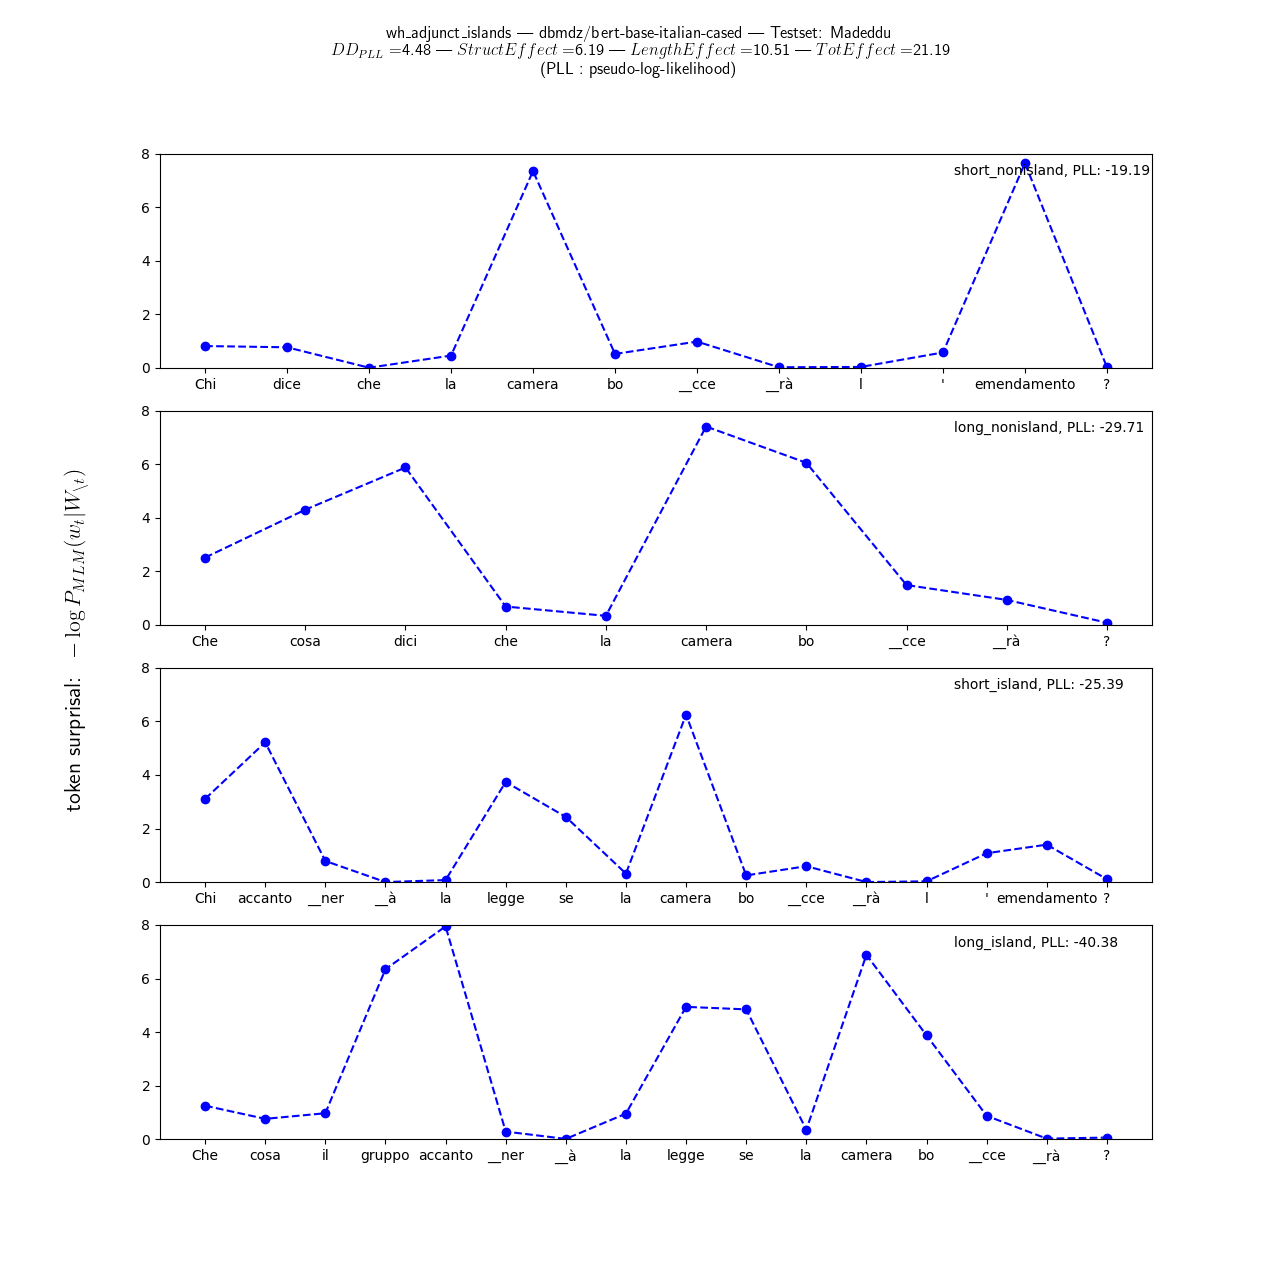
\includegraphics[width=1\textwidth]{images/Chapter1/token_surpisals/Madeddu_dbmdz_bert-base-italian-cased_wh_adjunct_islands_item_145.png} 
	\caption{Token surprisal of an adjunct island item, as scored by the Italian BERT.} 
	\label{fig:md_bert2b_adjunct_item_145_surprisals} 
	\medskip
\end{figure}

\begin{figure}[p]
	\centering
	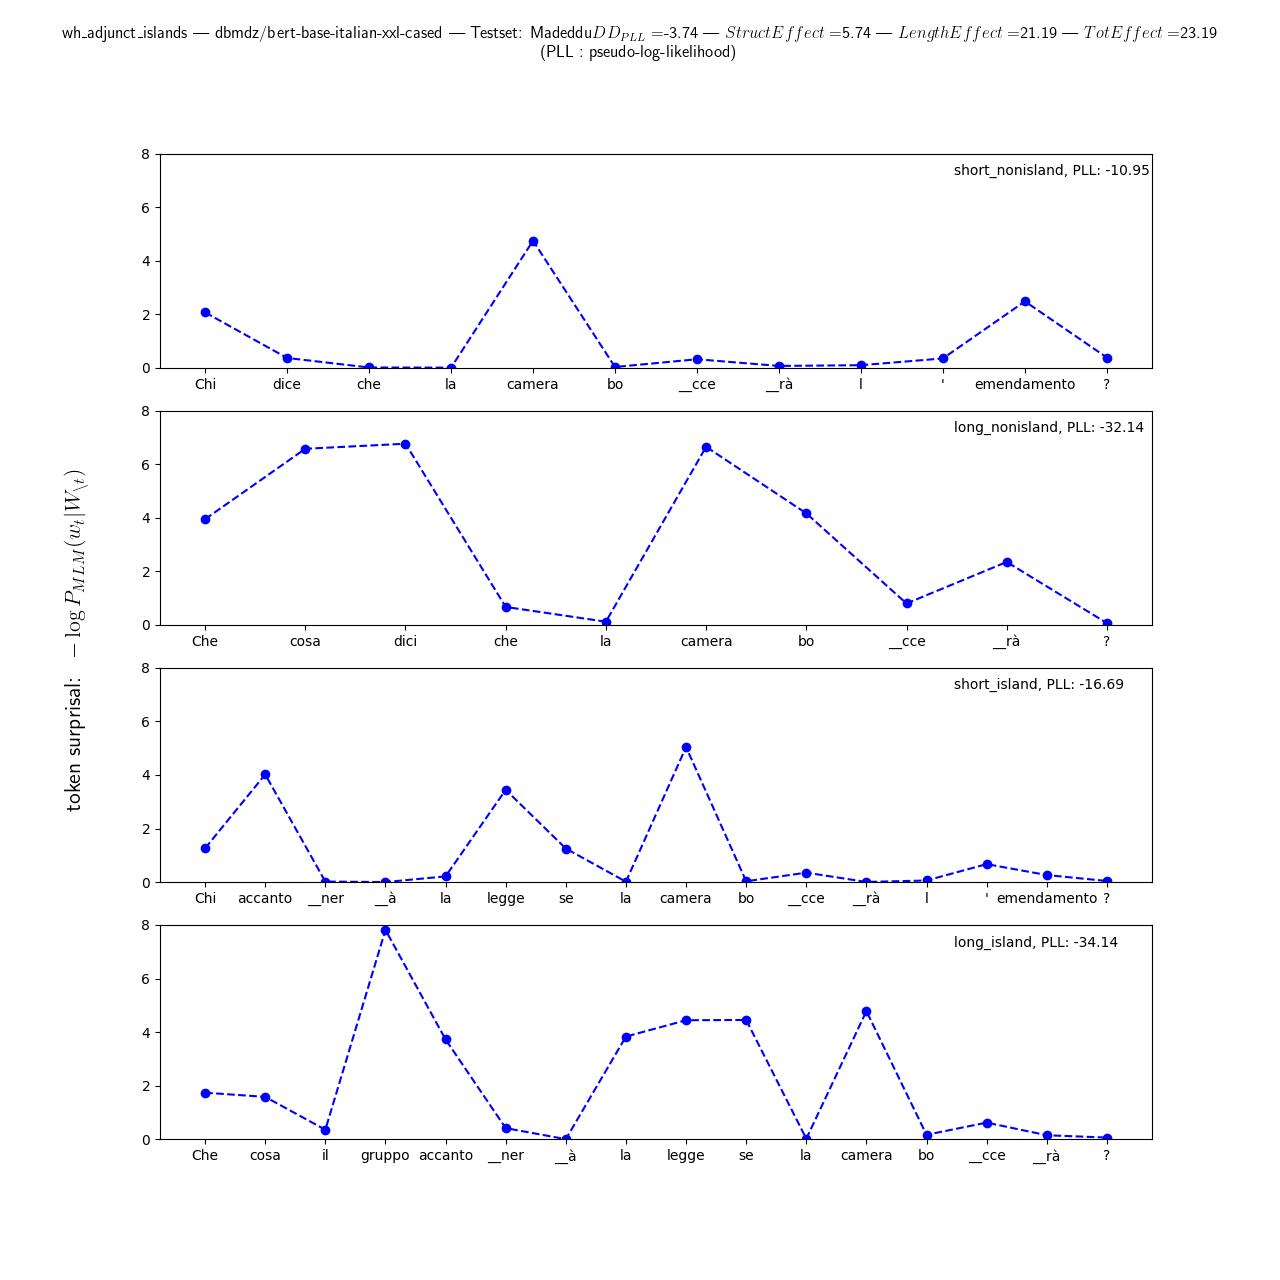
\includegraphics[width=1\textwidth]{images/Chapter1/token_surpisals/Madeddu_dbmdz_bert-base-italian-xxl-cased_wh_adjunct_islands_item_188.png} 
	\caption{Token surprisal of an adjunct island item, as scored by the Italian BERT XXL.} 
	\label{fig:md_bertxxl_adjunct_item_188_surprisals} 
	\medskip
\end{figure}

\begin{figure}[p]
	\centering
	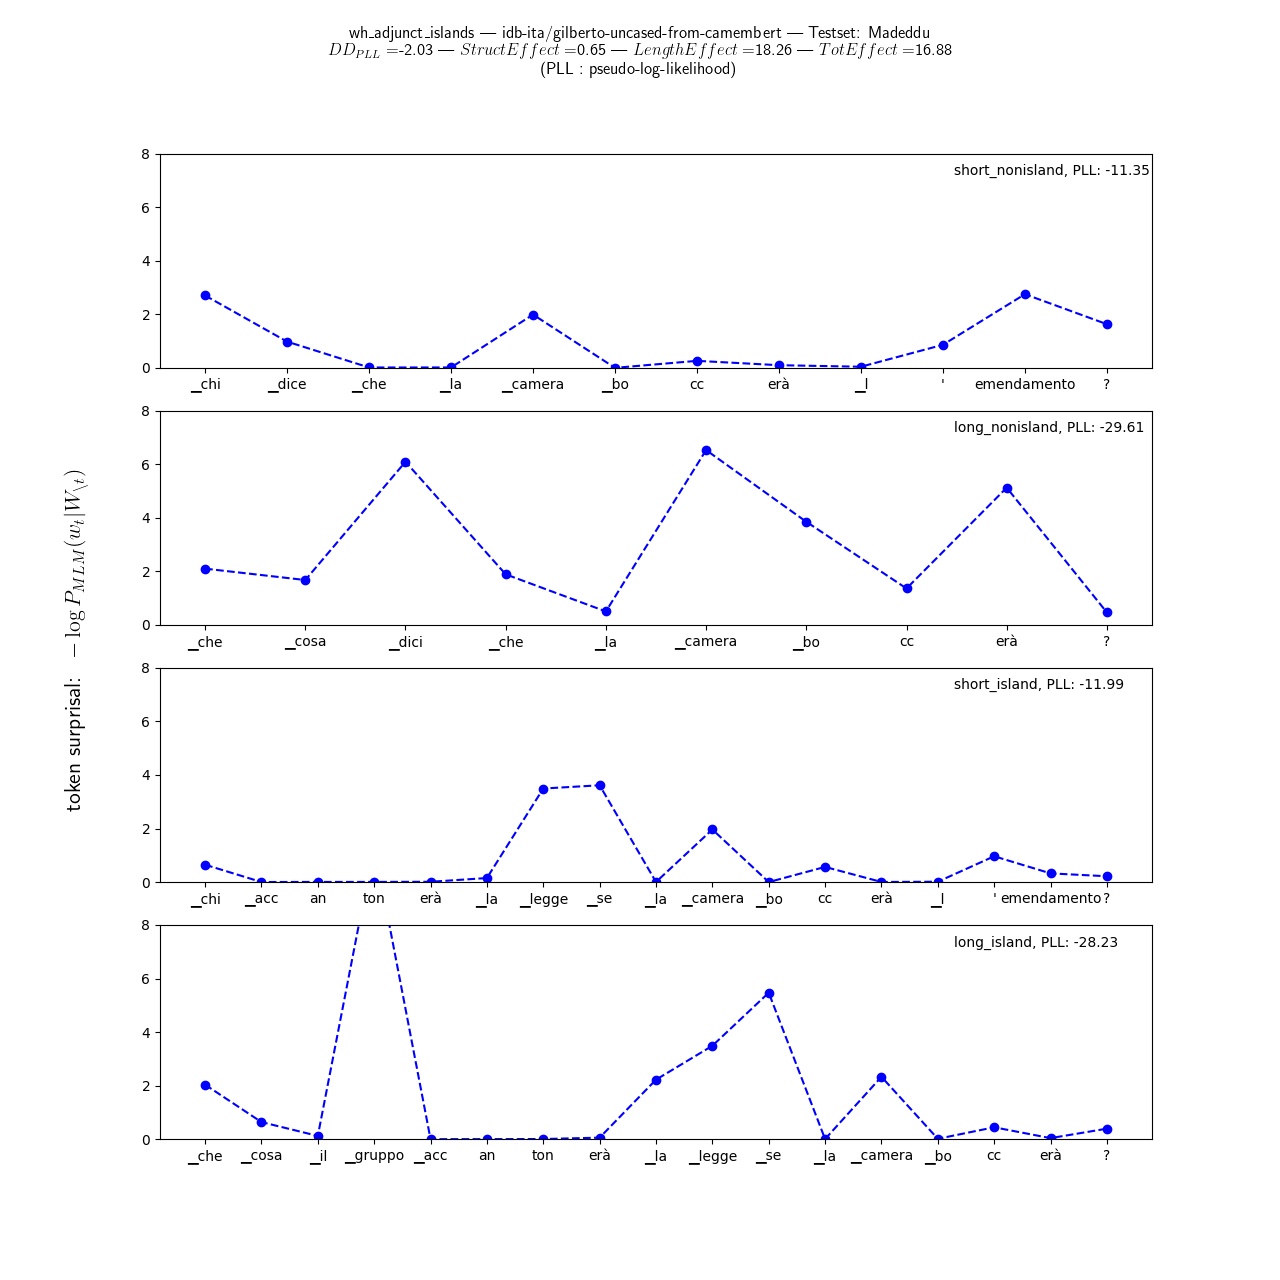
\includegraphics[width=1\textwidth]{images/Chapter1/token_surpisals/Madeddu_idb-ita_gilberto-uncased-from-camembert_wh_adjunct_islands_item_185.png} 
	\caption{Token surprisal of an adjunct island item, as scored by GilBERTo.} 
	\label{fig:md_gilberto_adjunct_item_185_surprisals} 
	\medskip
\end{figure}


\begin{figure}[p]
	\centering
	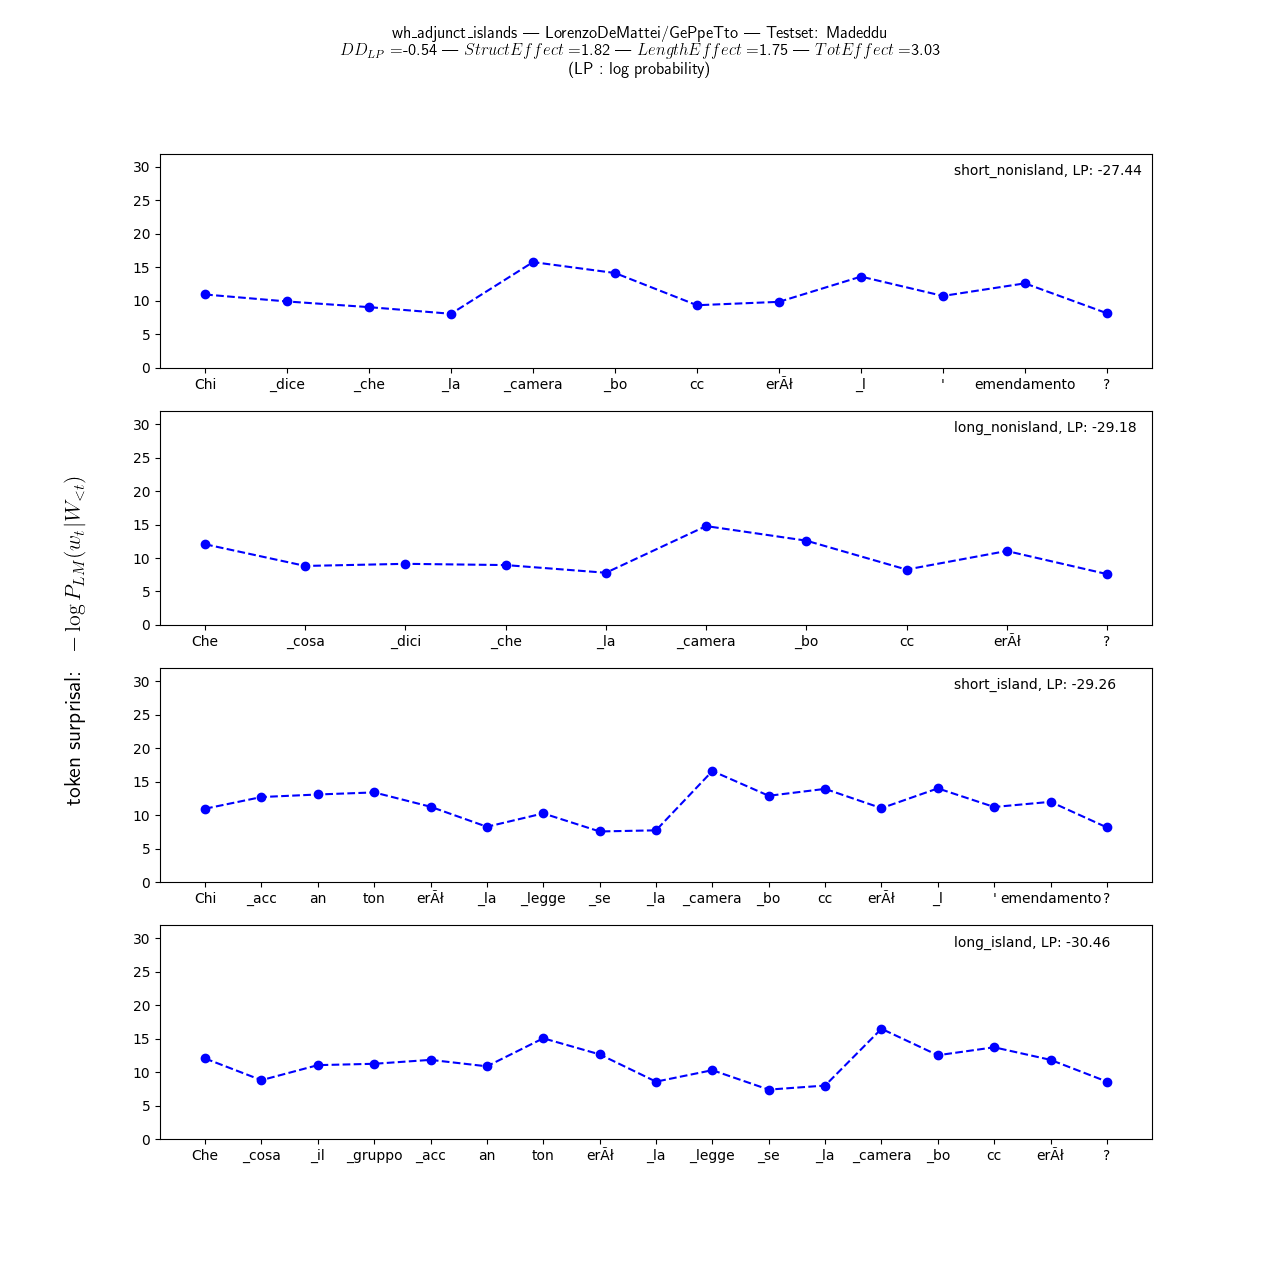
\includegraphics[width=1\textwidth]{images/Chapter1/token_surpisals/Madeddu_LorenzoDeMattei_GePpeTto_wh_adjunct_islands_item_163.png} 
	\caption{Token surprisal of an adjunct island item, as scored by GePpeTto.} 
	\label{fig:md_gpt_adjunct_item_163_surprisals} 
	\medskip
\end{figure}

In \autoref{fig:md_bert2b_adjunct_item_145_surprisals}, in the top sentence, we can see that BERT (the model trained with the least data), has not learned a strong association between "\textit{emendamento}" ("\textit{emendament}") and "\textit{la camera boccerà}" ("\textit{the lower chamber will reject}"), and for this reason the word gets a surprisal spike that highly influences the final sentence score. However, in the third sentence, we can see that the same word ("\textit{emendamento}") does not get the same spike, likely for the presence, far back at the beginning of the sentence, of the word "\textit{legge}" (\textit{law}), for which probably the model already has learned a strong association with "\textit{emendamento}".

Looking in \autoref{fig:md_bertxxl_adjunct_item_188_surprisals} at the plots for the same sentences from BERT XXL (trained with billions more data), we can see that the spikes in the first sentence for \textit{"camera"} ("\textit{lower chamber}") and  "\textit{emendamento}" ("\textit{emendament}"), have been much lowered compared to the previous model, likely because after 13B tokens of training data BERT has finally learned the association between these two words.

Factors like this can tilt the final factorial scores of an item, affecting its accuracy, and playing as a confound that masks these models responses to the syntactic phenomena we are interested. For these reasons, the sentences in a factorial item should be strictly balanced lexically, ideally having the same words (just in different order, as it is often the case in the BLiMP test suites), or at least have the same semantically full content words, with variations only in functional words. However, this is a non-trivial task, and designing targeted linguistic benchmarks in such a way, and for a comprehensive number of linguistic phenomena it's challenging and potentially very expensive. The approach adopted in works like BLiMP, to automatically generate the items from templates, is not necessarily less demanding, since for more complex phenomena there is also an increase in the the complexity of the templates and of the annotation schema for the selectional preferences of each word in the sampling lexicon such as the one used in BLiMP.

Back to our initial question, on why BERT XXL, the model trained with the most data (13B tokens), has a 6+ points drop in accuracy for adjunct islands, compared with BERT and GilBERTo? Looking at the token surprisals in \autoref{fig:md_bert2b_adjunct_item_145_surprisals}, \ref{fig:md_bertxxl_adjunct_item_188_surprisals}, and \ref{fig:md_gilberto_adjunct_item_185_surprisals}, we can see that for the bottom ungrammatical sentence ("\textit{Che cosa il gruppo accantonerà se la camera boccerà}") ("\textit{What will the group set aside if the lower chamber rejects?}"), all models have a spike for the word \textit{"se"} ("\textit{if}"), which is a critical region that could indicate that the model detects a grammatical influency. All three models also show a surprisal spike at this word in the 2nd sentence from the bottom ("\textit{Chi accantonerà la legge se la camera boccerà l'emendamento?}") ("\textit{Who will set aside the law if the lower chamber rejects?}"), but these spikes are lower compared to the previous sentence. This could indicate that the models correctly respond with higher surprisals to the presence of an island construct, and also correctly, they further increase this surprisal when there is a violation of the extraction constraint given by this construct, showing that they have learned this type of island effects. However, in these plots we can notice that these surprisal spikes at the word \textit{"se"} ("\textit{if}"), are not clearly reflected in the final PLL scores of each sentence, because of the presence of larger surprisal spikes from other words, likely due to more prominent semantic effects.

Looking at the plot of the plots for the average scores in \autoref{fig:md_bert_lp}, we can see that the lines between sentences show very close average acceptability values between sentences with and without and island structure and a dependency of the same distance, with a relatively small slope difference between the two lines (when they are parallel, it indicates that the model is insensitive to that type of island effect). Therefore we can hypothesize that the lexical semantic confounding factors observed in the previous factors can easily shift the overall factorial DD score above or below the defined threshold of the success criterion for accuracy ($DD > 0$). This could partially explain why all the three BERT-based models showed relatively poor performance (64-72\%) in this type of islands. GPT-2, on the other hand, which scored at 98\%, shows a more marked separation and difference in slope between the two lines\autoref{fig:md_gpt_penlp} .

% confounds: avoid questions; or better do set of tests with and without questions; because the most challenging scenarios must not be escluded from evaluating language models; if a model show not to be able to learn a syntactic phenomenon when in the interrogative form, this shows a significant limitation of its generalizations .. although processing complexity also lowers acceptability scores in humans..

% Chi dice che la camera boccerà l'emendamento?
% Madeddu_dbmdz_bert-base-italian-xxl-cased_wh_adjunct_islands_item_188.png
% Madeddu_idb-ita_gilberto-uncased-from-camembert_wh_adjunct_islands_item_185.png
% Madeddu_dbmdz_bert-base-italian-cased_wh_adjunct_islands_item_145.png

\subsubsection{Subject islands}

For subject islans, the token surprisals in Fig. .. - ..

In \autoref{fig:md_gpt_subject_item_152_surprisals} we observe the non-optimal sub-word units splits performed by the tokenizer used by GPT-2: the out-of-vocabulary (OOV) word \textit{"impoverito"} (\textit{"impoverished"}) has been split into \textit{imp-ov-erito}, which clearly cannot take advantage of the semantically informative root \textit{"pover-"} ("\textit{poor}"). \citet{bostrom2020byte} found that sub-word splitting algorithms like BPE % does Gpt/geppetto use BPE?
are non optimal, and that a more linguistically plausible sub-word tokenization (with units that resemble more traditional morphemes), increases performance in downstream tasks. We argue that an optimal subword units tokenization should be a key element of a deep neural language models, since all the representations that these models learn are learned on top of these building blocks. We can expect that non optimal building blocks starting points will limit the possible generalizations and the patterns that these models are able to learn on top of them. The split of a training corpus in tokens is a strong signal that conveys a lot of information, and finding more optimal sub-word unit splits can also be though of as a form of regularization that avoids overfitting phenomena on the probability distribution of the training corpus.

\begin{figure}[p]
	\centering
	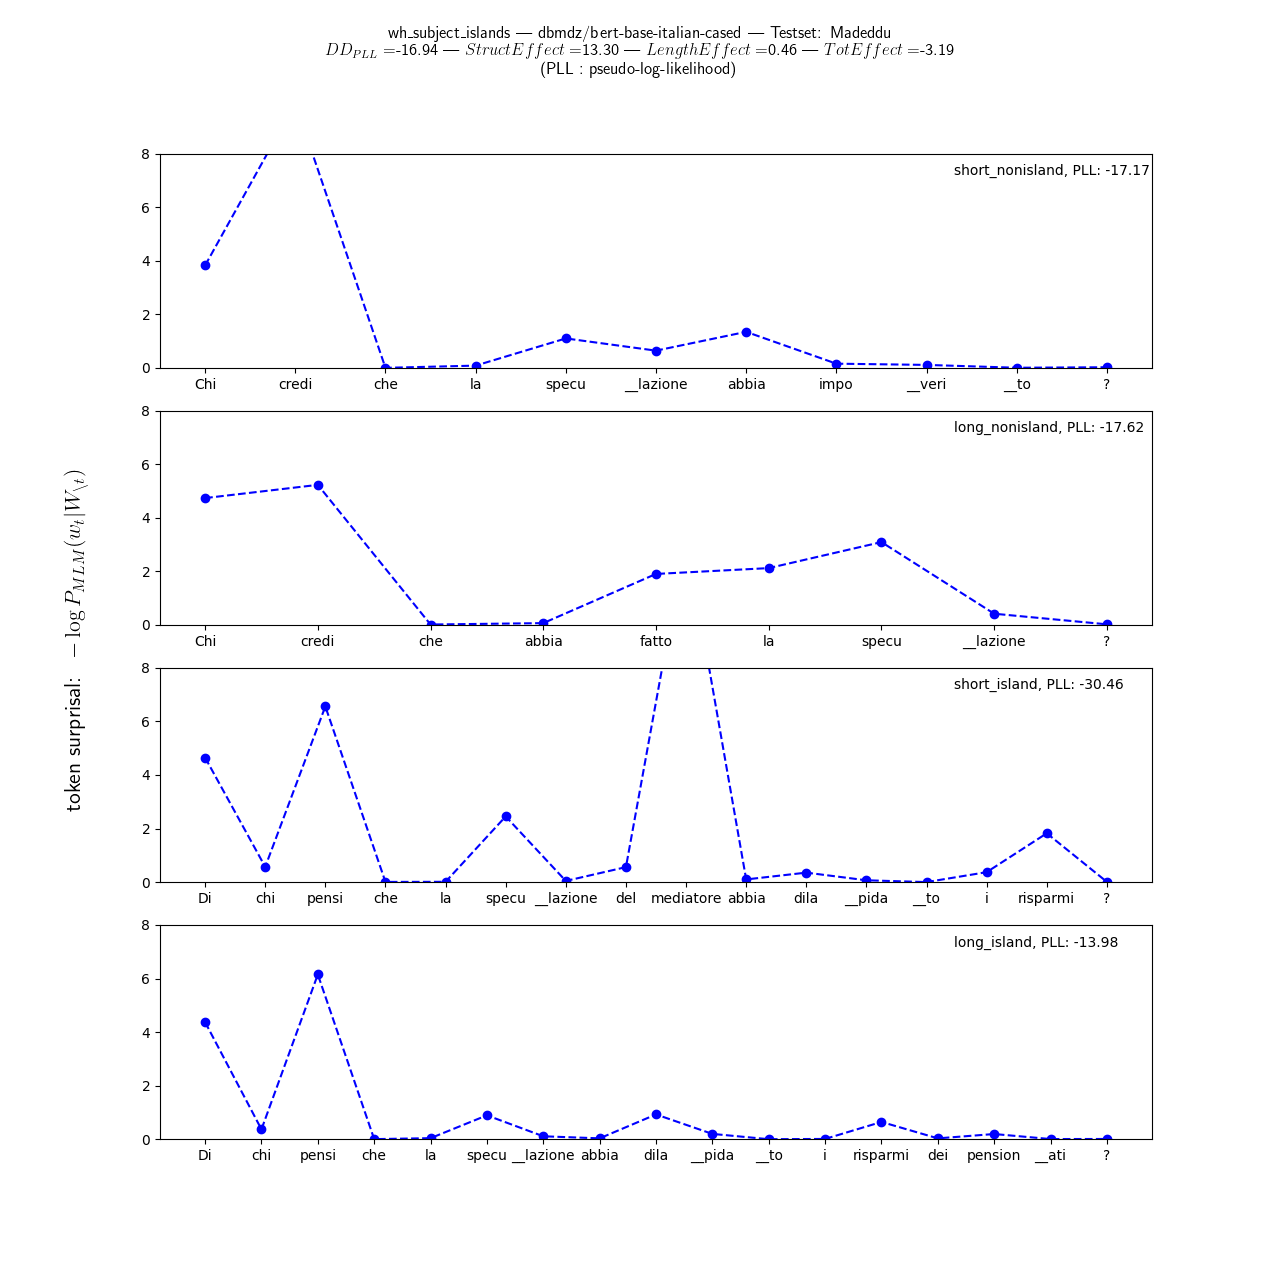
\includegraphics[width=1\textwidth]{images/Chapter1/token_surpisals/Madeddu_dbmdz_bert-base-italian-cased_wh_subject_islands_item_196.png} 
	\caption{Token surprisal of an subject island item, as scored by the Italian BERT.} 
	\label{fig:md_bert2b_subject_item_196_surprisals} 
	\medskip
\end{figure}

\begin{figure}[p]
	\centering
	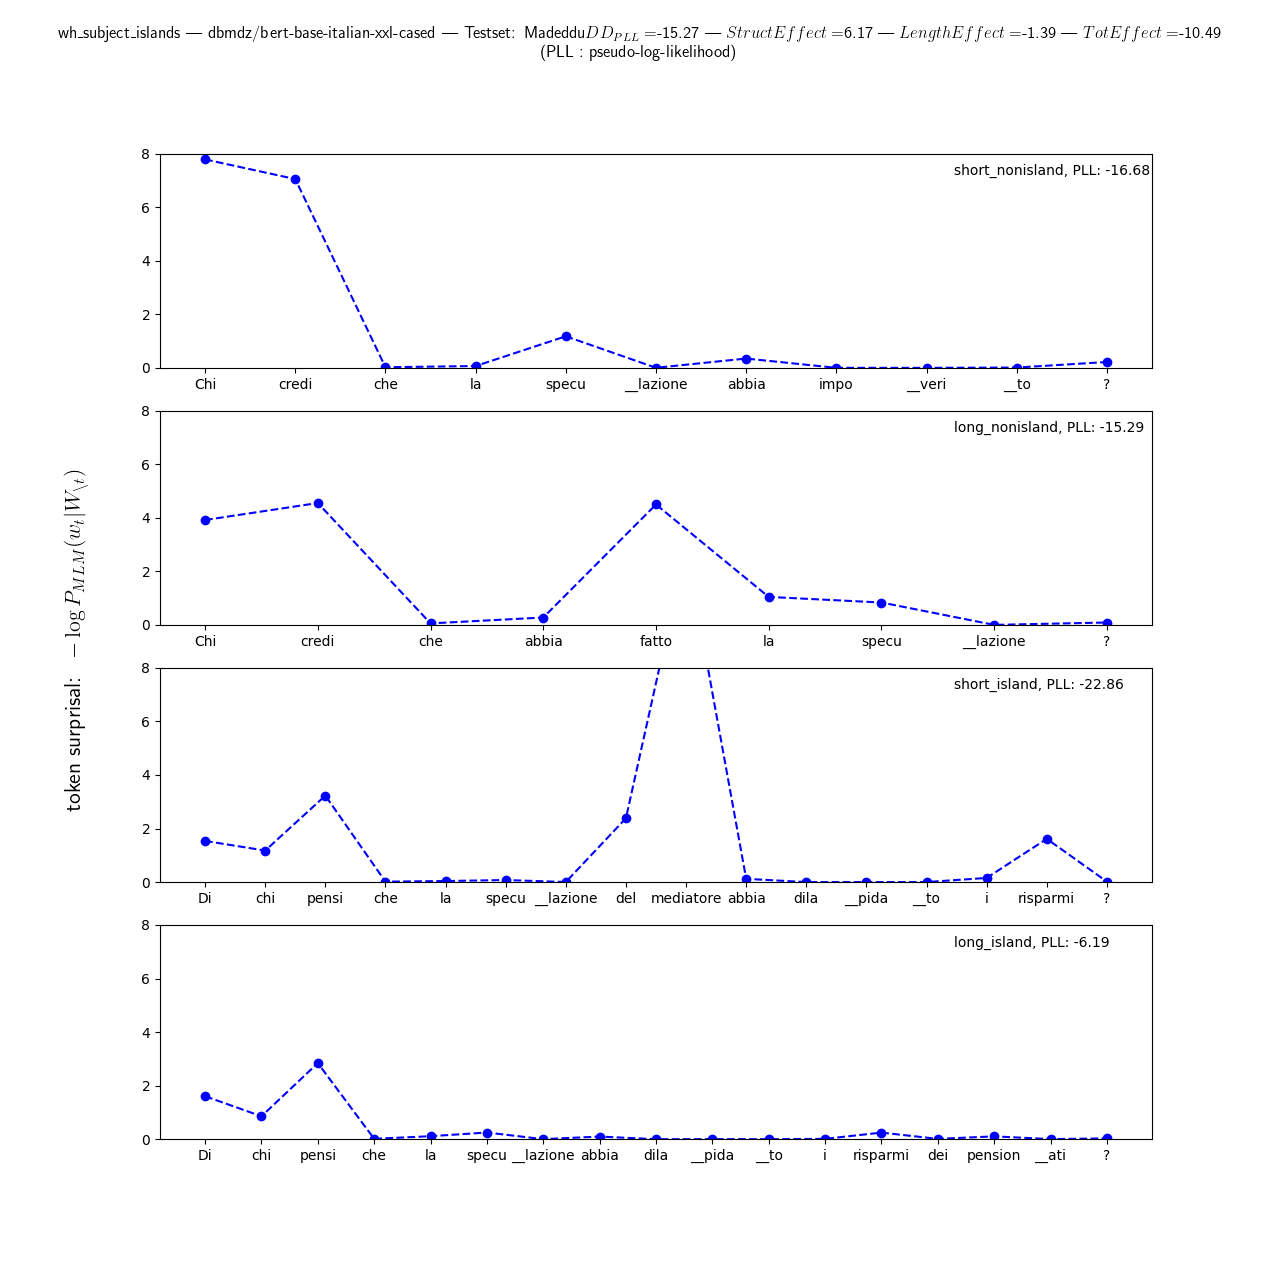
\includegraphics[width=1\textwidth]{images/Chapter1/token_surpisals/Madeddu_dbmdz_bert-base-italian-xxl-cased_wh_subject_islands_item_198.png} 
	\caption{Token surprisal of an subject island item, as scored by the Italian BERT XXL.} 
	\label{fig:md_bertxxl_subject_item_198_surprisals} 
	\medskip
\end{figure}

\begin{figure}[p]
	\centering
	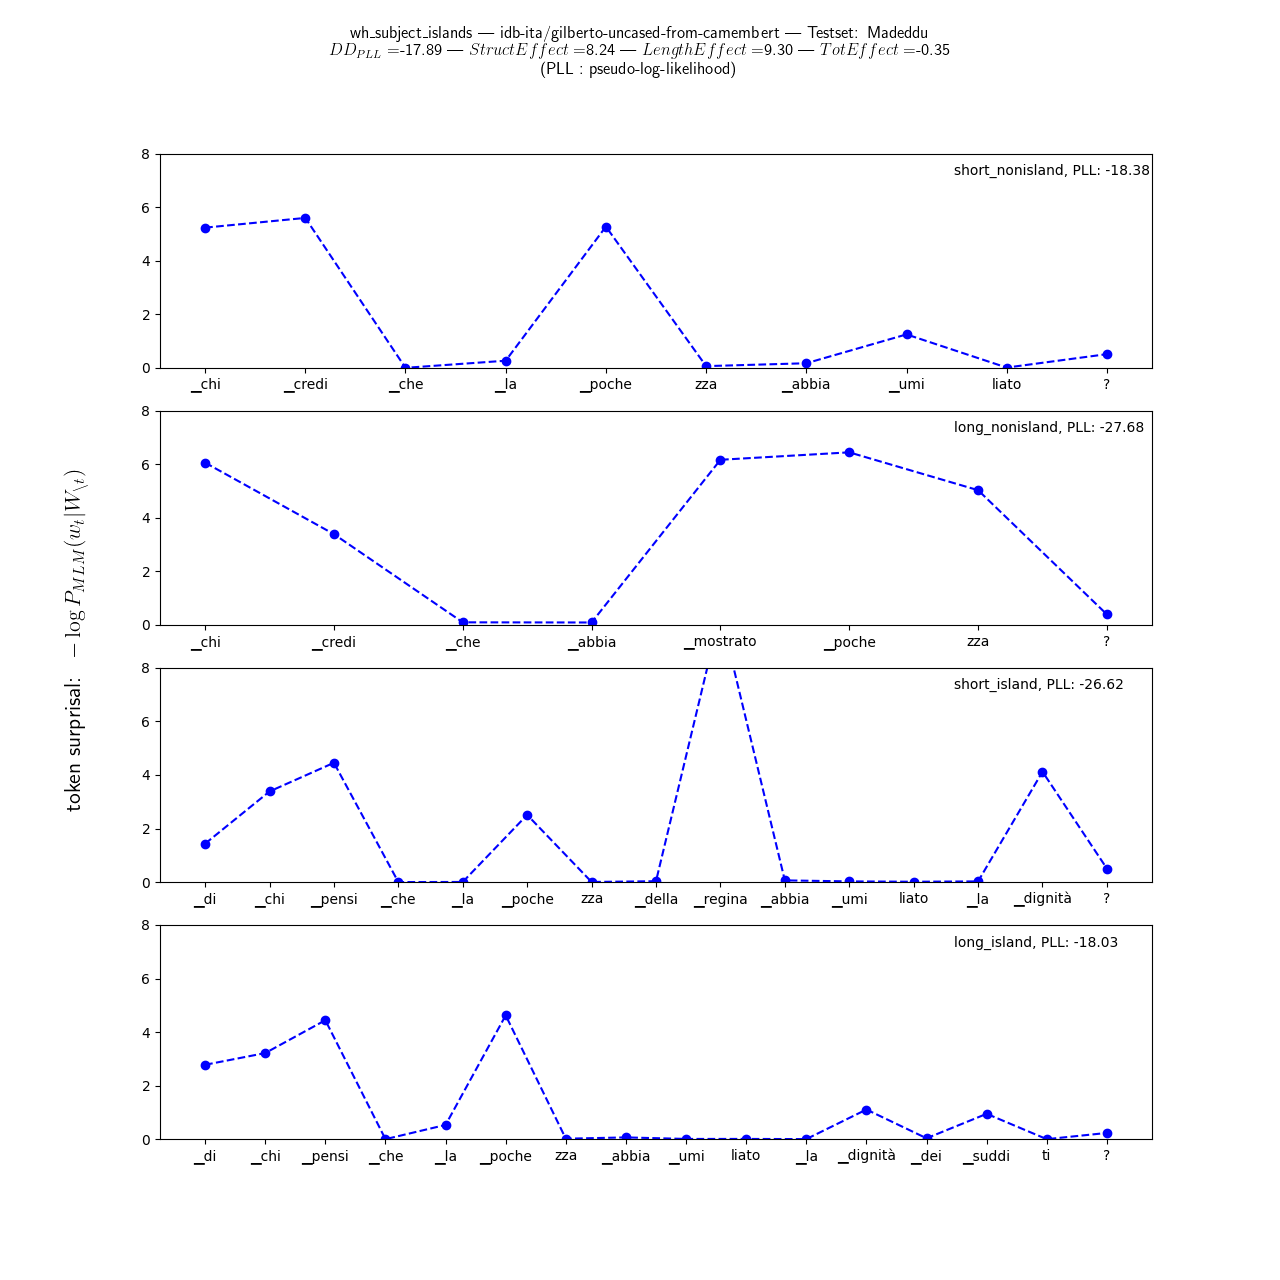
\includegraphics[width=1\textwidth]{images/Chapter1/token_surpisals/Madeddu_idb-ita_gilberto-uncased-from-camembert_wh_subject_islands_item_199.png} 
	\caption{Token surprisal of an subject island item, as scored by GilBERTo.} 
	\label{fig:md_gilberto_subject_item_199_surprisals} 
	\medskip
\end{figure}


\begin{figure}[p]
	\centering
	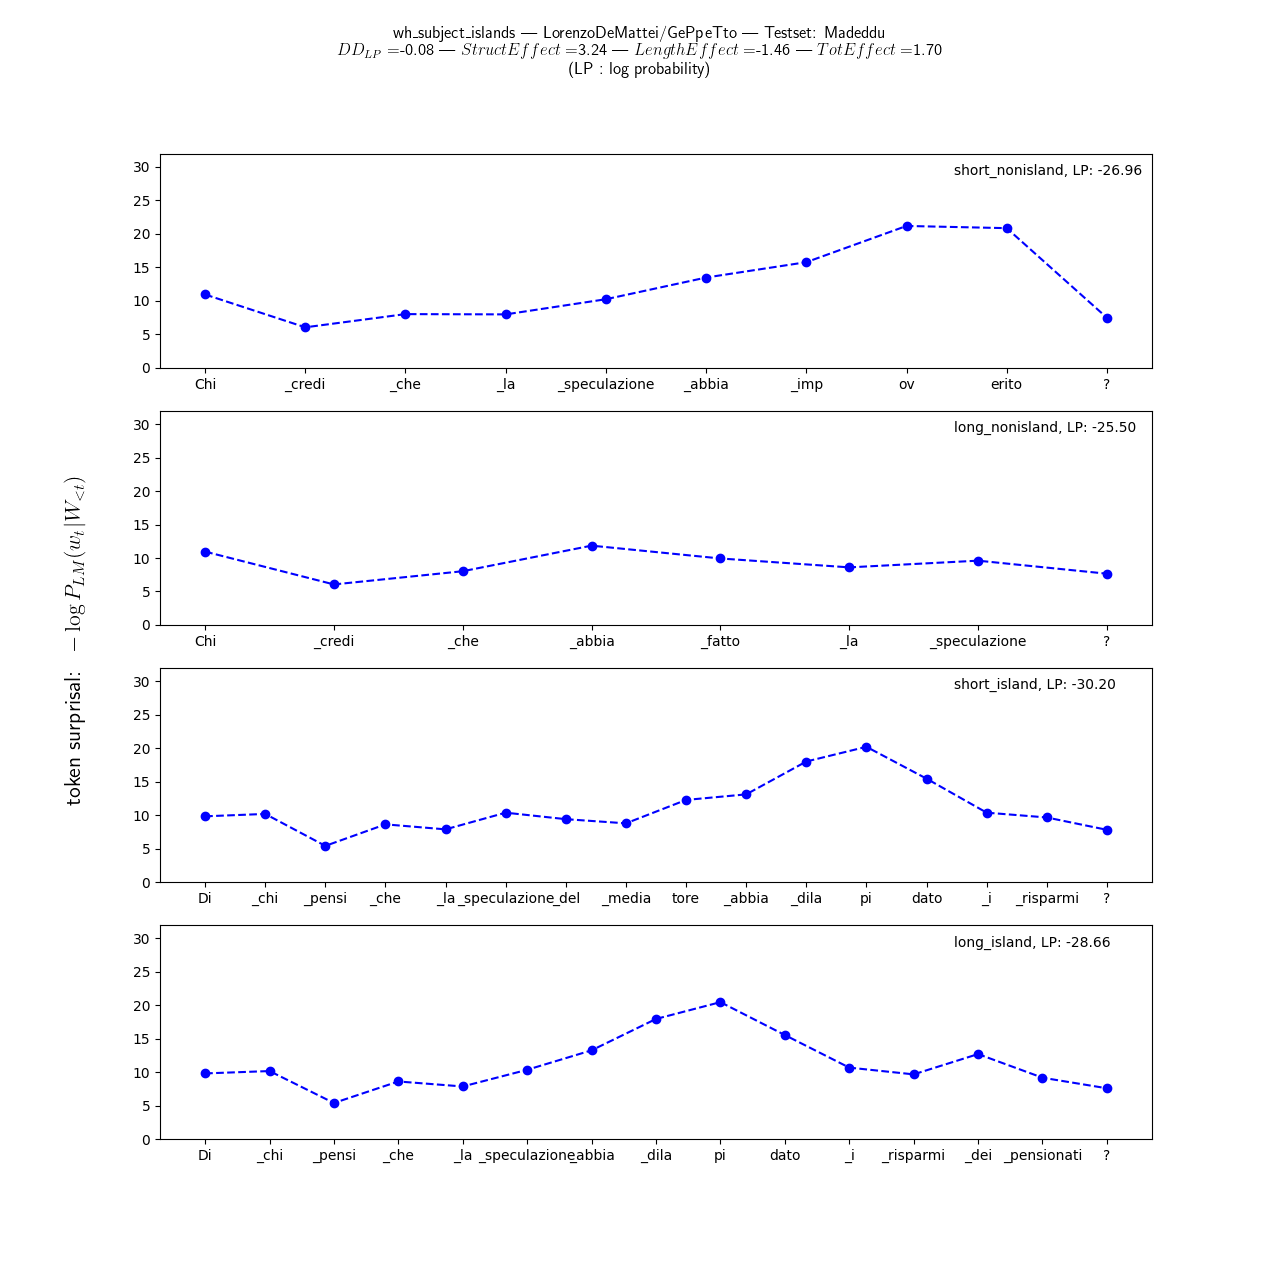
\includegraphics[width=1\textwidth]{images/Chapter1/token_surpisals/Madeddu_LorenzoDeMattei_GePpeTto_wh_subject_islands_item_152.png} 
	\caption{Token surprisal of an subject island item, as scored by GePpeTto.} 
	\label{fig:md_gpt_subject_item_152_surprisals} 
	\medskip
\end{figure}

\subsubsection{Complex NP islands}

\begin{figure}[p]
	\centering
	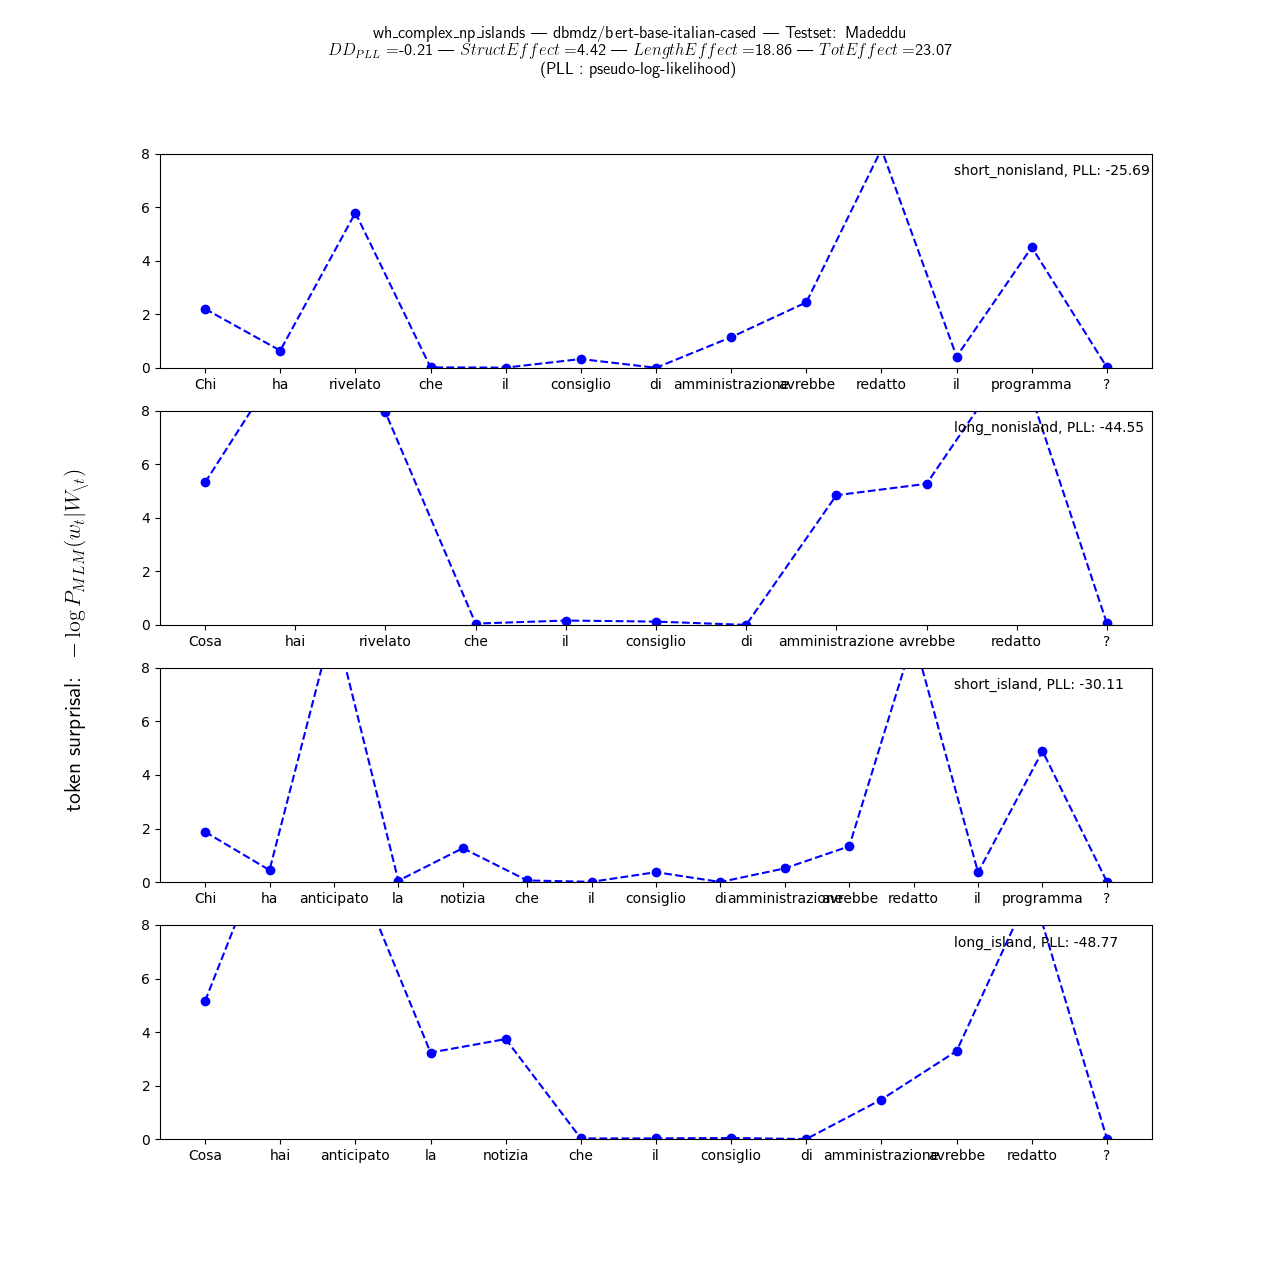
\includegraphics[width=1\textwidth]{images/Chapter1/token_surpisals/Madeddu_dbmdz_bert-base-italian-cased_wh_complex_np_islands_item_173.png} 
	\caption{Token surprisal of a complex NP island item, as scored by the Italian BERT.} 
	\label{fig:md_bert2b_complex_np_item_173_surprisals} 
	\medskip
\end{figure}

\begin{figure}[p]
	\centering
	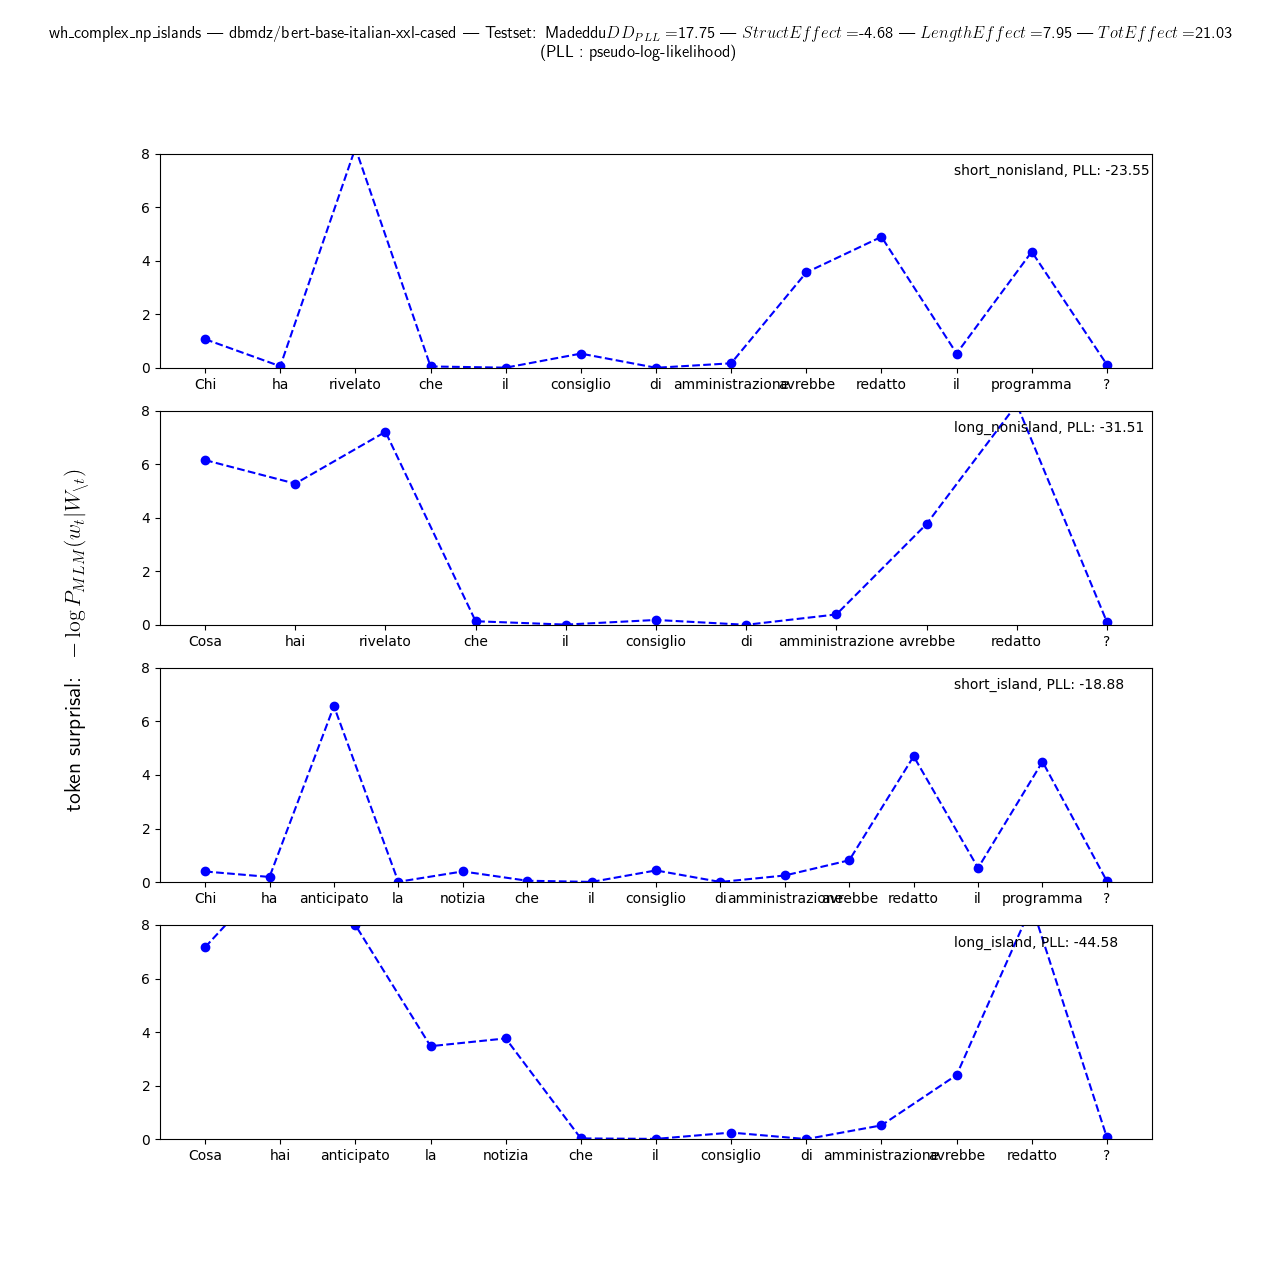
\includegraphics[width=1\textwidth]{images/Chapter1/token_surpisals/Madeddu_dbmdz_bert-base-italian-xxl-cased_wh_complex_np_islands_item_32.png} 
	\caption{Token surprisal of a complex NP island item, as scored by the Italian BERT XXL.} 
	\label{fig:md_bertxxl_complex_np_item_32_surprisals} 
	\medskip
\end{figure}

\begin{figure}[p]
	\centering
	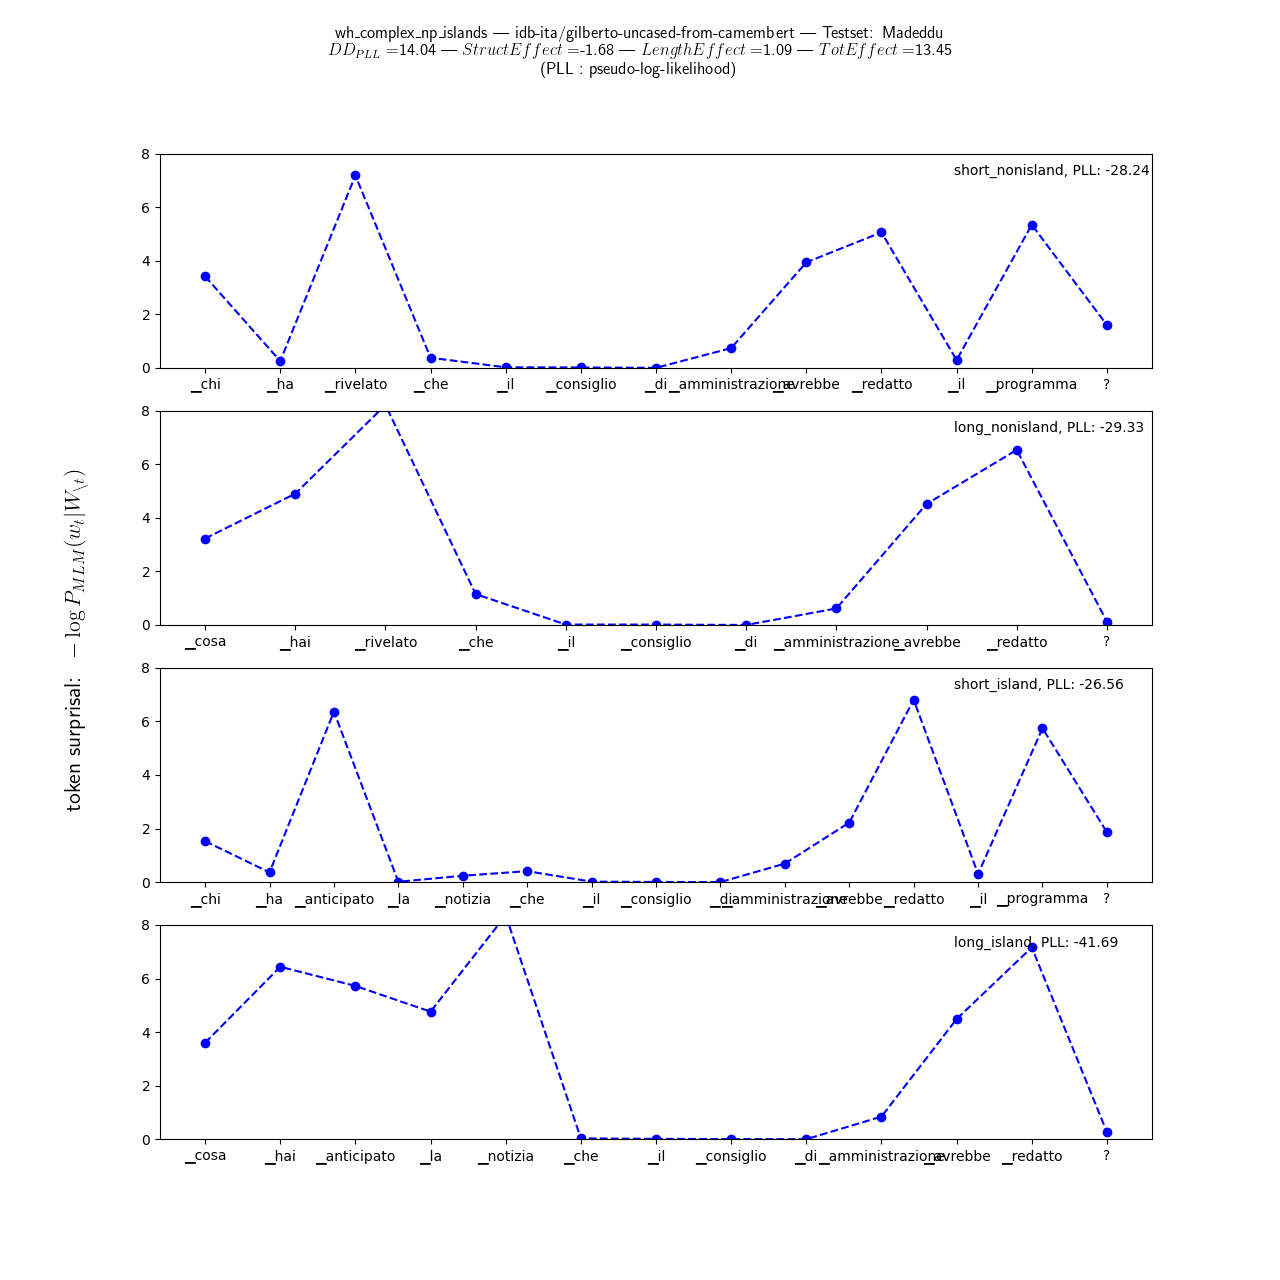
\includegraphics[width=1\textwidth]{images/Chapter1/token_surpisals/Madeddu_idb-ita_gilberto-uncased-from-camembert_wh_complex_np_islands_item_88.png} 
	\caption{Token surprisal of a complex NP island item, as scored by GilBERTo.} 
	\label{fig:md_gilberto_complex_np_item_88_surprisals} 
	\medskip
\end{figure}

\begin{figure}[p]
	\centering
	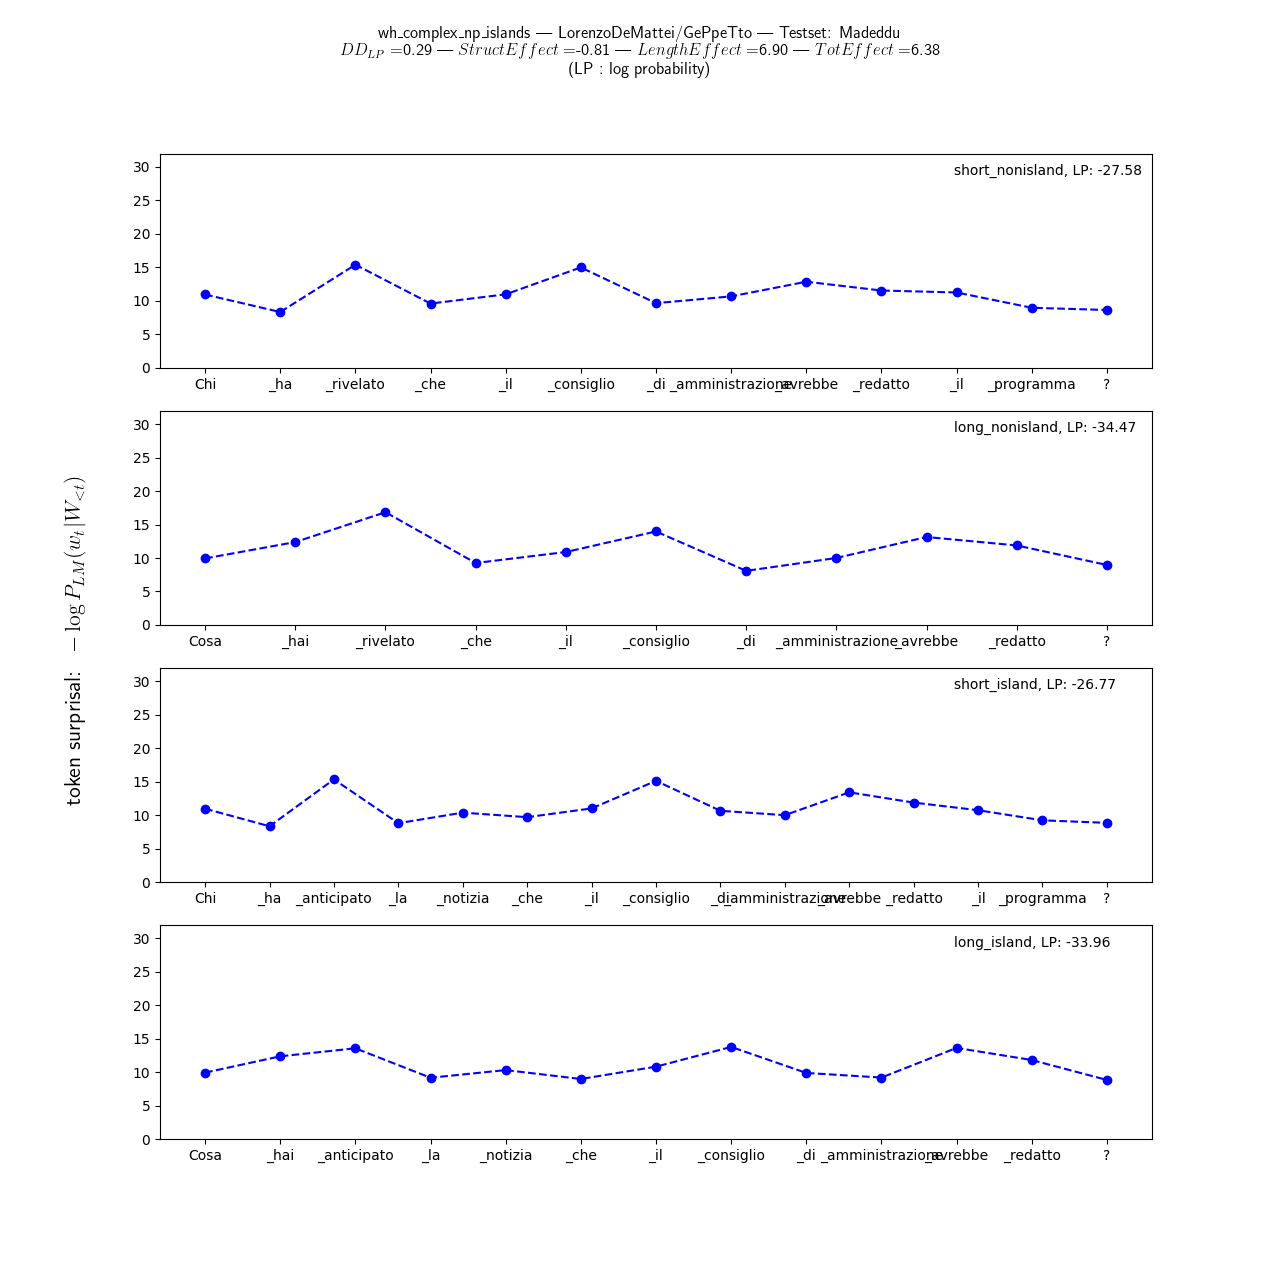
\includegraphics[width=1\textwidth]{images/Chapter1/token_surpisals/Madeddu_LorenzoDeMattei_GePpeTto_wh_complex_np_islands_item_142.png} 
	\caption{Token surprisal of a complex NP island item, as scored by GePpeTto.} 
	\label{fig:md_gpt_complex_np_item_142_surprisals} 
	\medskip
\end{figure}

\subsubsection{Whether islands}


Plateau at 100\% accuracy between 2-11B trainin tokens. It's not clear from te surprisal plots what is driving this change, but it seems due to the fact that the baseline acceptable sentence (\textsc{short-nonisland}) get a lower acceptability in BERT XXL. We can notice the strange phenomenon that BERT XXL gets a high surprisal (much higher than BERT) on the word "\textit{affitto}" ("\textit{rent}"). Again this is seems another case of semantic phenomena having a prevailing confounding effect, that could mask the effec of syntactic ones.

\begin{figure}[p]
	\centering
	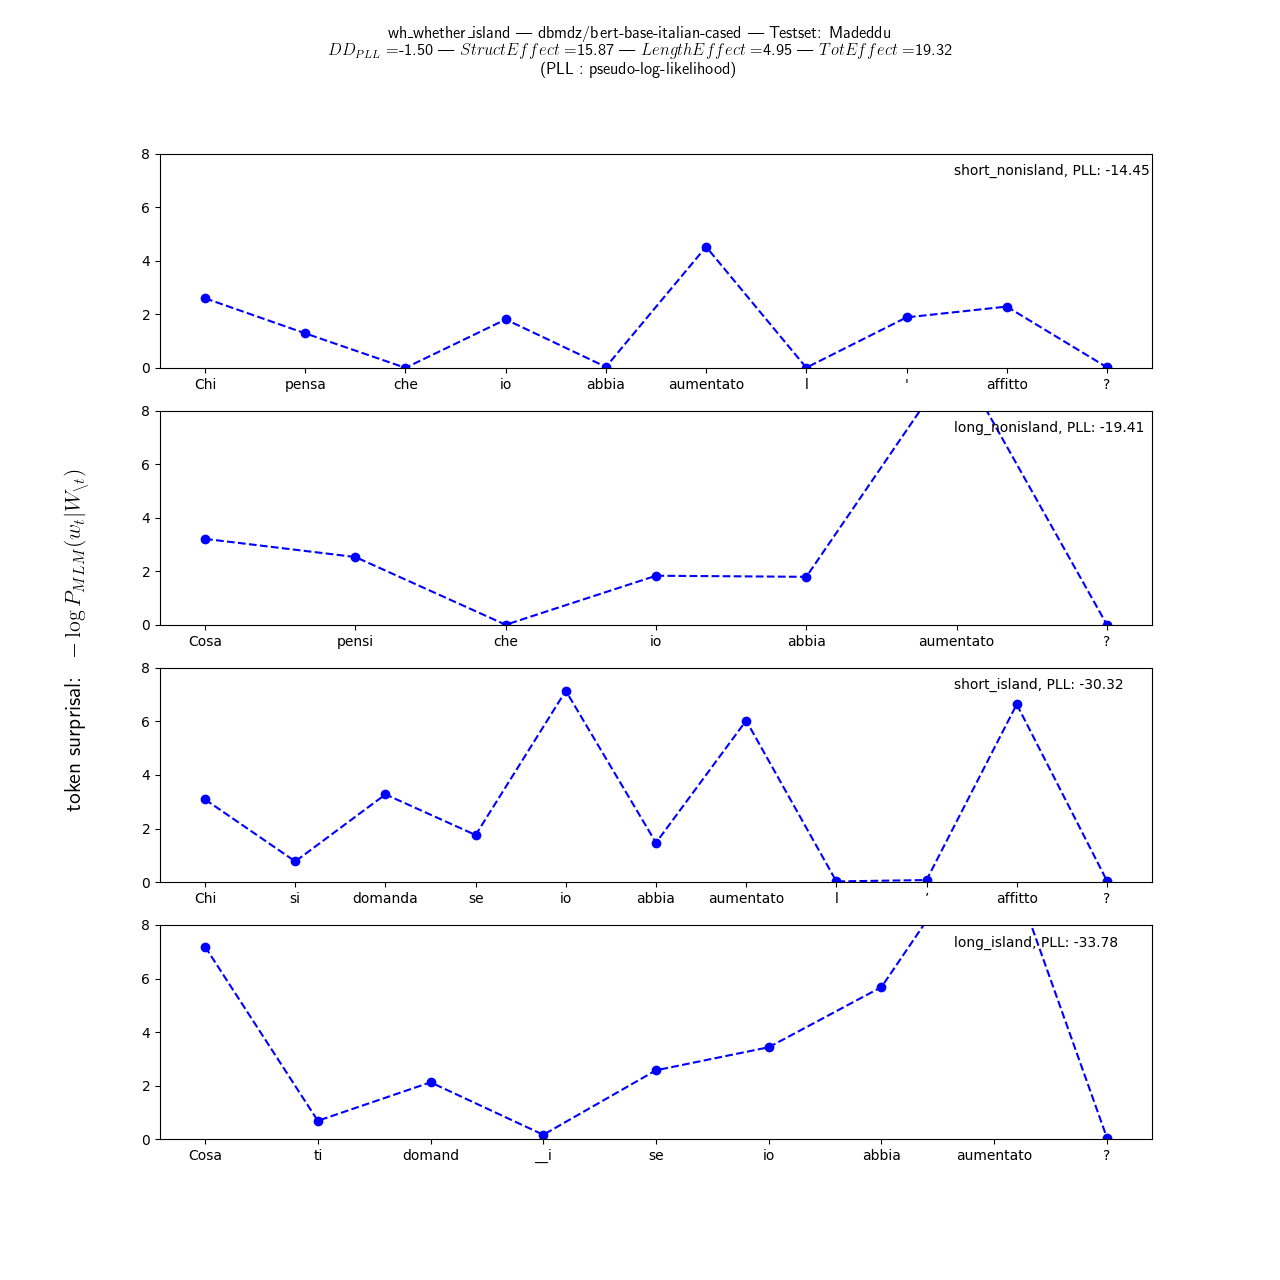
\includegraphics[width=1\textwidth]{images/Chapter1/token_surpisals/Madeddu_dbmdz_bert-base-italian-cased_wh_whether_island_item_180.png} 
	\caption{Token surprisal of a whether island item, as scored by the Italian BERT.} 
	\label{fig:md_bert2b_whether_item_180_surprisals} 
	\medskip
\end{figure}

\begin{figure}[p]
	\centering
	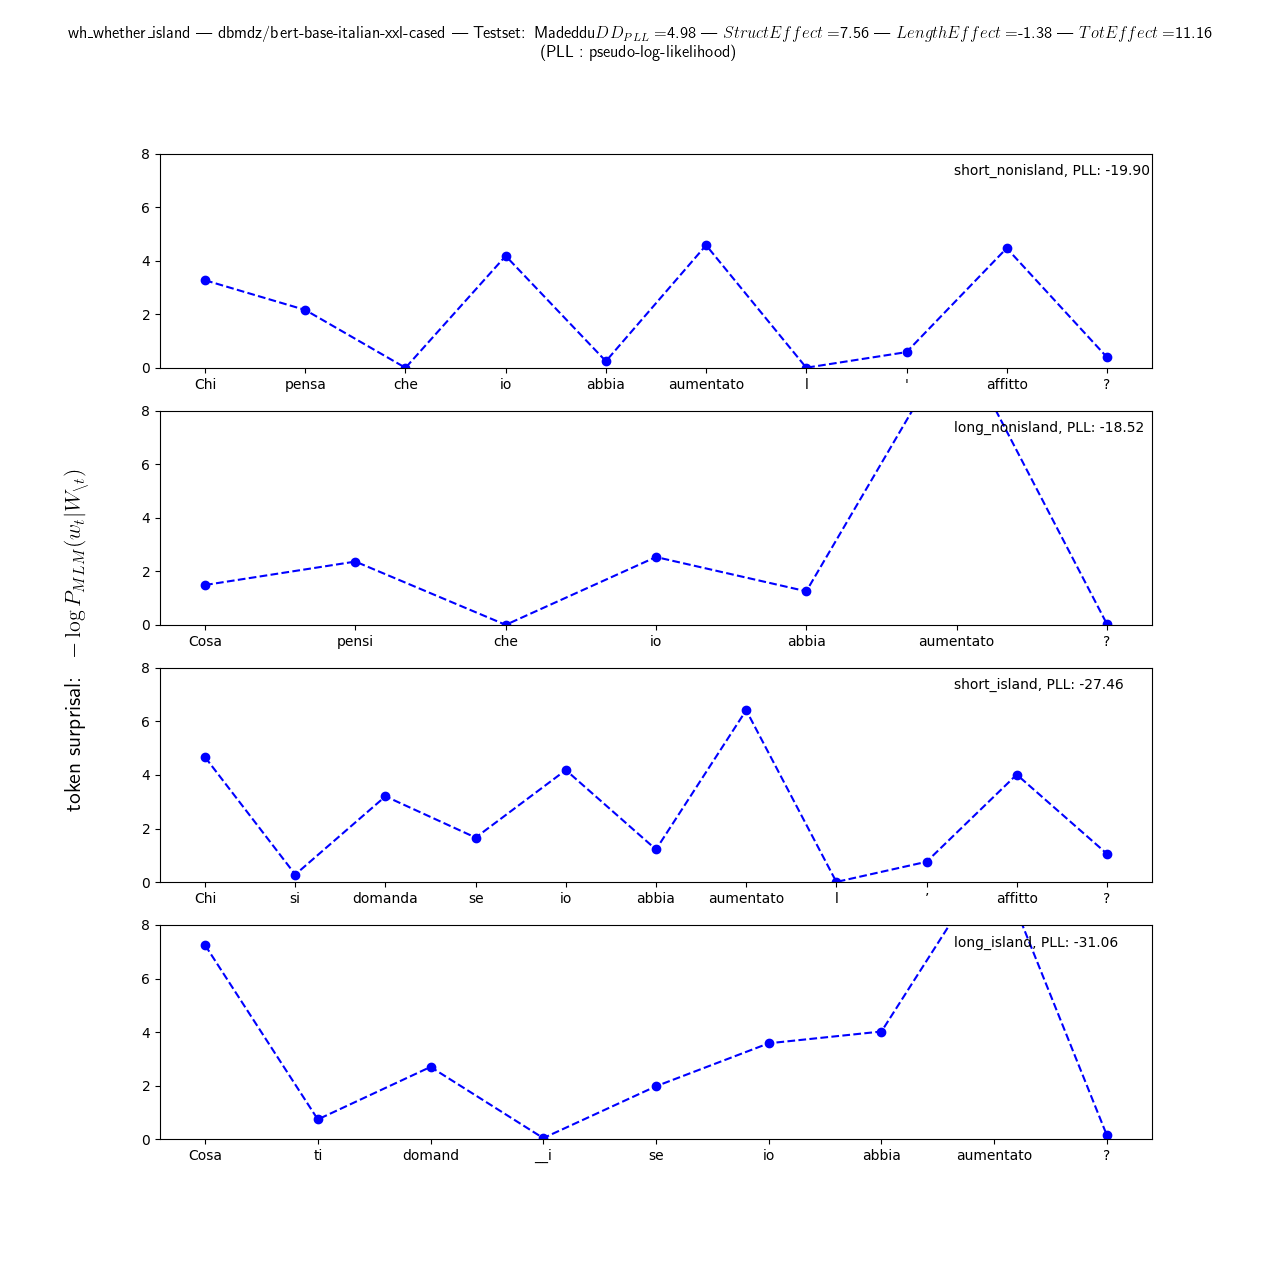
\includegraphics[width=1\textwidth]{images/Chapter1/token_surpisals/Madeddu_dbmdz_bert-base-italian-xxl-cased_wh_whether_island_item_156.png} 
	\caption{Token surprisal of a whether island item, as scored by the Italian BERT XXL.} 
	\label{fig:md_bertxxl_whether_item_156_surprisals} 
	\medskip
\end{figure}

\begin{figure}[p]
	\centering
	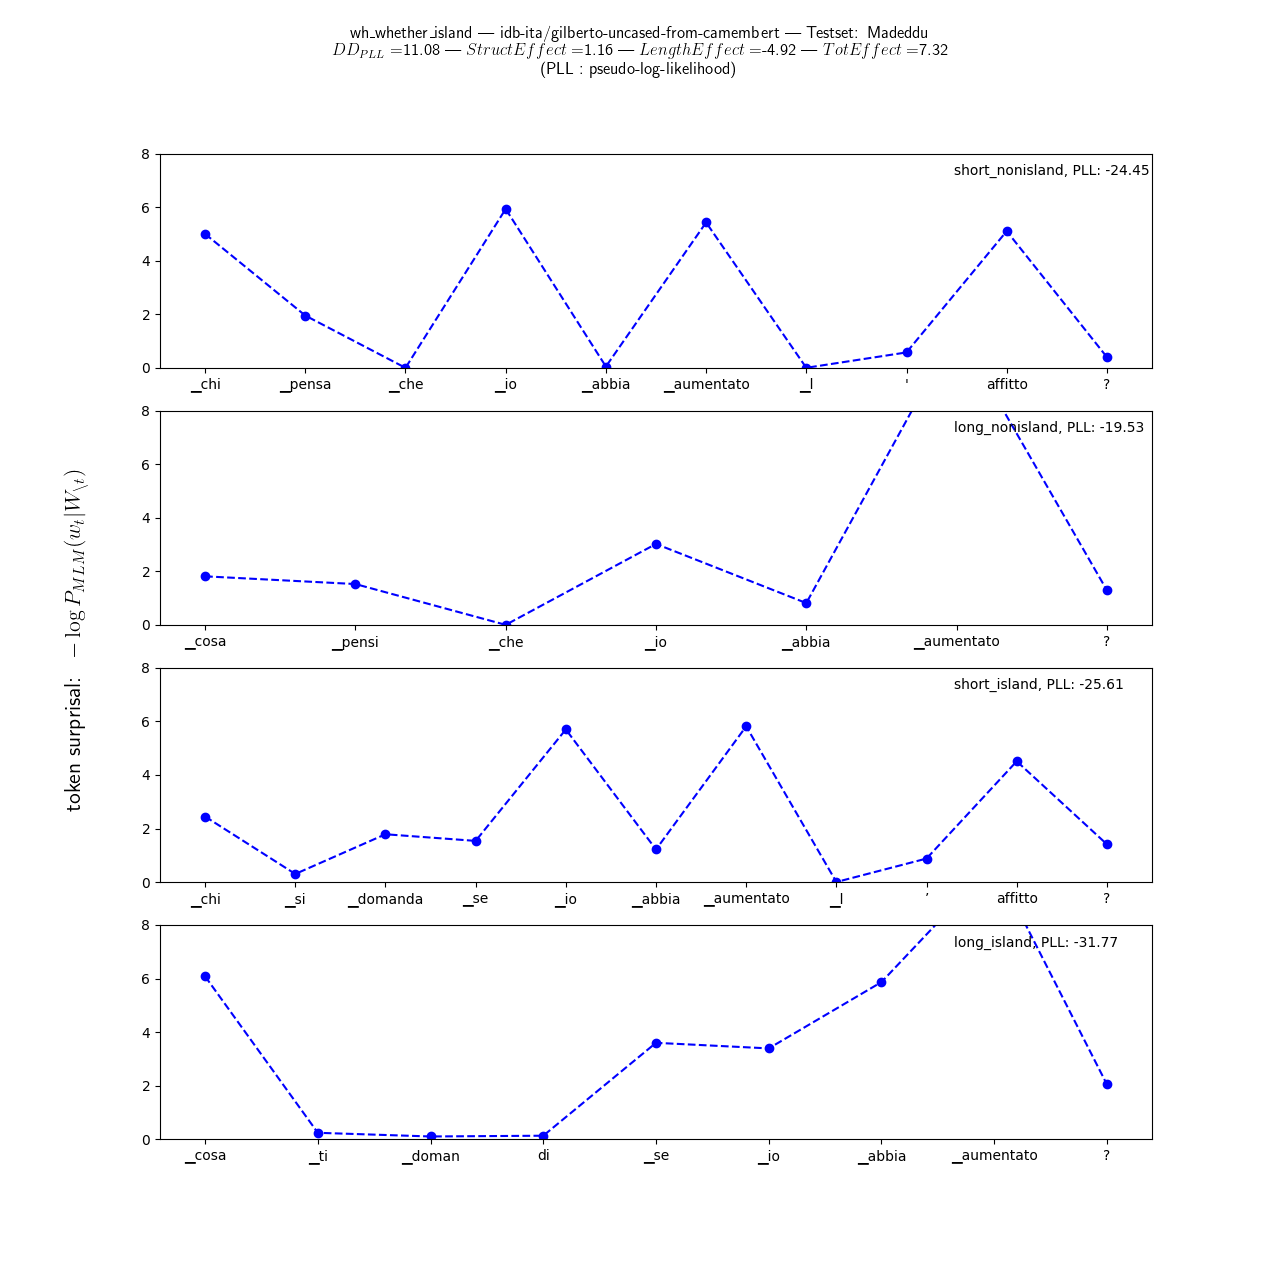
\includegraphics[width=1\textwidth]{images/Chapter1/token_surpisals/Madeddu_idb-ita_gilberto-uncased-from-camembert_wh_whether_island_item_121.png} 
	\caption{Token surprisal of a whether island item, as scored by GilBERTo.} 
	\label{fig:md_gilberto_whether_item_121_surprisals} 
	\medskip
\end{figure}

\begin{figure}[p]
	\centering
	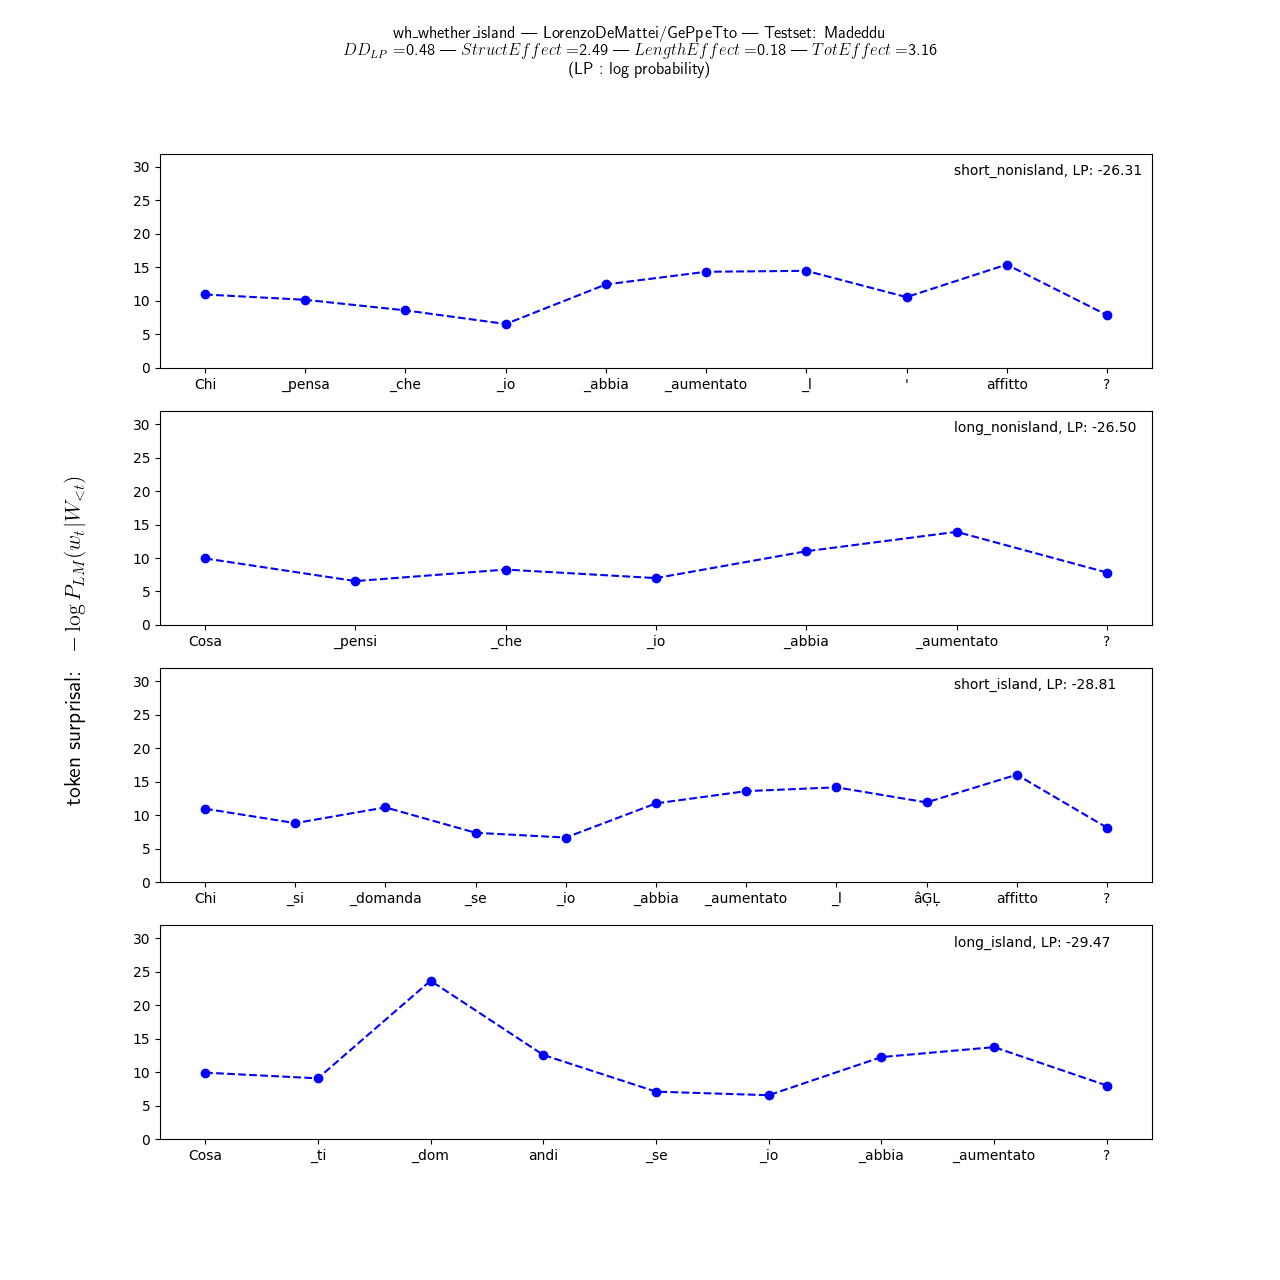
\includegraphics[width=1\textwidth]{images/Chapter1/token_surpisals/Madeddu_LorenzoDeMattei_GePpeTto_wh_whether_island_item_135.png} 
	\caption{Token surprisal of a whether island item, as scored by GePpeTto.} 
	\label{fig:md_gpt_whether_item_135_surprisals} 
	\medskip
\end{figure}

\subsection{Qualitative analysis (continued)}

In Fig. \ref{fig:sprouse_humans} we see the original plots from \citet{sprouse2016experimental}, on results collected from Italian subjects for wh-dependencies islands. Figures \ref{fig:md_gpt_penlp} to \ref{fig:md_gilberto_lp} show the plots we obtained for the same types of island constructs and wh-dependencies, with our test suite (that has a format similar to that of Sprouse et al.), on three Italian language models: the GPT-2-based GePpeTto \citep{de2020geppetto}\footnote{https://huggingface.co/LorenzoDeMattei/GePpeTto}, BERT (base-xxl version)\footnote{https://huggingface.co/dbmdz/bert-base-italian-xxl-cased} and the RoBERTa-based GilBERTo\footnote{https://huggingface.co/idb-ita/gilberto-uncased-from-camembert}. For comparison, we also show in Fig.\ref{fig:sprouse_gpt_penlp}-\ref{fig:sprouse_bert2b_lp} plots on the scores given by the three above language models on the original test suites by \citet{sprouse2016experimental}.

The y axis represents the structure condition (island or non-island). The x axis (for whether, adjunct, and complex NP islands) represents the dependency distance: short-distance extraction from the matrix clause, or long-distance extraction from the embedded clause. The x axis for subject islands, instead, as discussed in \autoref{sec:testsuite_design}, represents extraction of the object from the embedded clause, or extraction of the subject from the embedded clause. The "non-island" line, marked in solid blue, connects the values for the two sentences without the island structure. The orange dotted line is the "island line", connecting the values for the two sentences with the island structure.

% in the two datasets the stimuli are similar, but there are differences (for instance, out adjunct islands test suite includes temporal adjuncts, while in the Sprouse one includes only conditional adjuncts, as noted in section ..).

% todo, and move to appropriate section: discuss/clarify about the different labeling of plots: short/long distance dependencies, vs matrix/embedded or subject/object



We can see that the plots for whether (top-left plot of each figure), adjunct (bottom-right), and subject islands (bottom-left) from the GPT-2 model (\autoref{fig:md_gpt_penlp}) show some similarities with those obtained on human subjects (\autoref{fig:sprouse_humans}), but also some significant differences.


% (assess a smaller model trained only on 100M tokens?)
% gilberto vs bertbasexxl training tokens (11B vs 13B)
% add dbmdz/bert-base-italian-cased (trained on 2B tokens, while the xxl-cased version was trained on 13B tokens). To make the point on how much data needed, and showing if going from 2B to 13B is needed even for syntax.
% this is in particular interesting for subject islands, since in the current results there is a trend of improvement from
% and for complex np, this might be the reason for the low performance of geppetto (46%)
% could disambiguate/clarify results on adjuncts
% see if perf on whether decreases ..

% compare bertbasexxl with gilberto: gilberto different tokenizer, different type of training data.. but same architecture?


%\subsection{GePpeTto}
%\subsubsection{GePpeTto with PenLP (from softmax model output)}

% todo: 2 facing pages with 4 figures: sprouse paper plots, then 3 models plots (geppetto, bert, GilBERTo) on the madeddu dataset
% after this 2 pages with 3 figures for the plots on the 3 models and the sprouse testsuite, for comparison
% \begin{figure}[p]
% \begin{figure}[ht]
	
\begin{figure}[p]
	\centering
	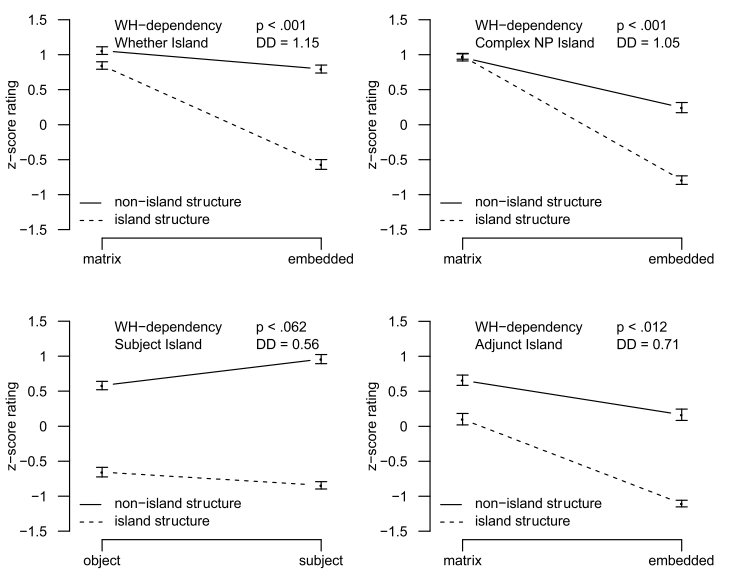
\includegraphics[width=1\textwidth]{images/Chapter1/Plot_1_Sprouse_paper.png} 
	\caption{Plots of average acceptability scores from humans taken from \citep{sprouse2016experimental}}
		\label{fig:sprouse_humans} 
		\medskip
\end{figure}	
	
\begin{figure}[p]
	\centering
	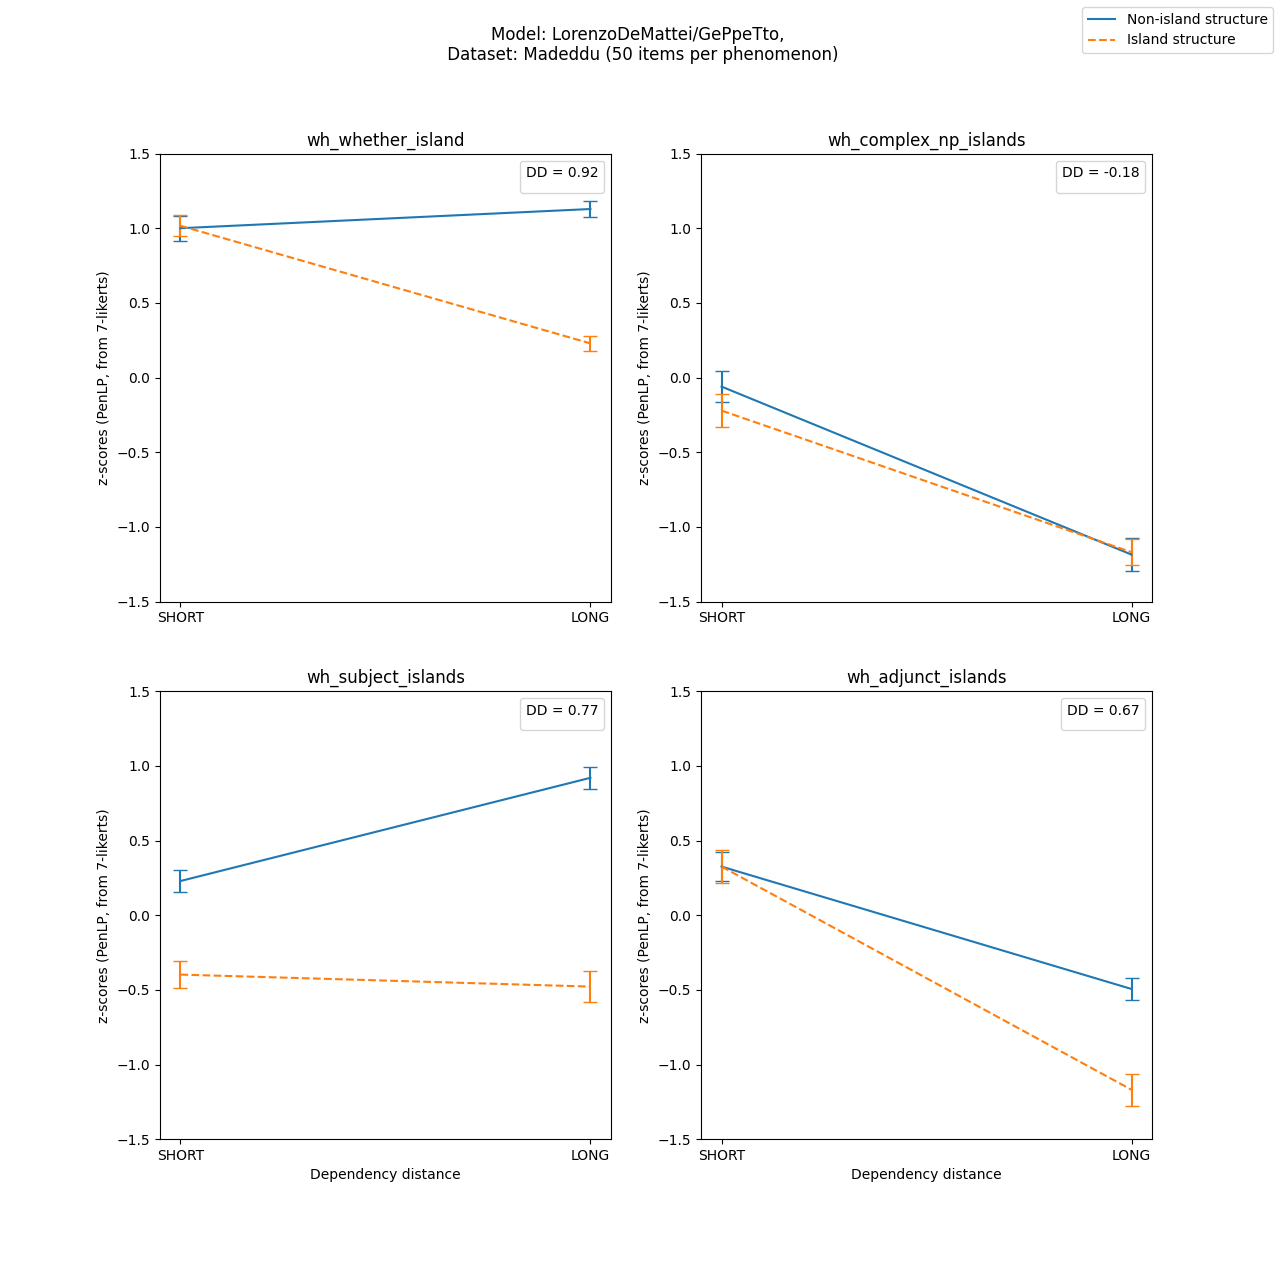
\includegraphics[width=1\textwidth]{images/Chapter1/Madeddu_wh_LorenzoDeMattei_GePpeTto_PenLP-zscores-likert-2022-09-14_h15m12s44.png} 
	\caption{Plots of average acceptability scores from GePpeTto, on the test suites developed for the present thesis.}
	\label{fig:md_gpt_penlp} 
	\medskip
\end{figure}	


\begin{figure}[p]
	\centering
	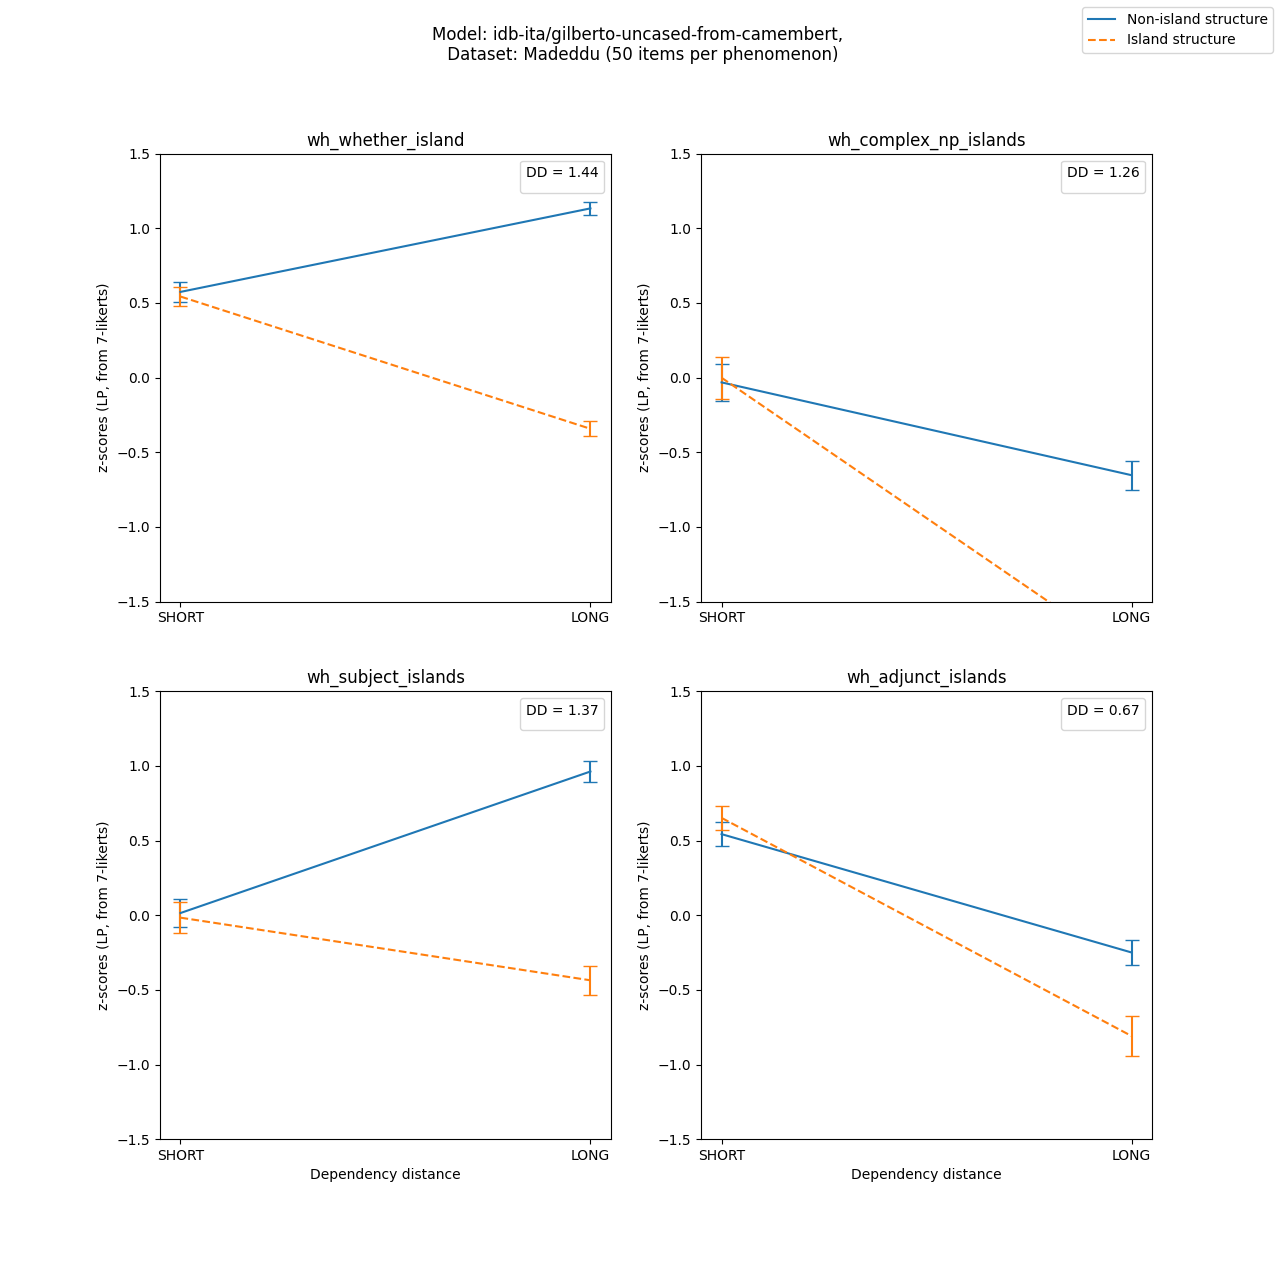
\includegraphics[width=1\textwidth]{images/Chapter1/Madeddu_wh_idb-ita_gilberto-uncased-from-camembert_LP-zscores-likert-2022-09-16_h10m28s27.png} 
	\caption{Plots of average acceptability scores from GilBERTo, on the test suites developed for the present thesis.}
	\label{fig:md_gilberto_lp} 
	\medskip
\end{figure}	


\begin{figure}[p]
	\centering
	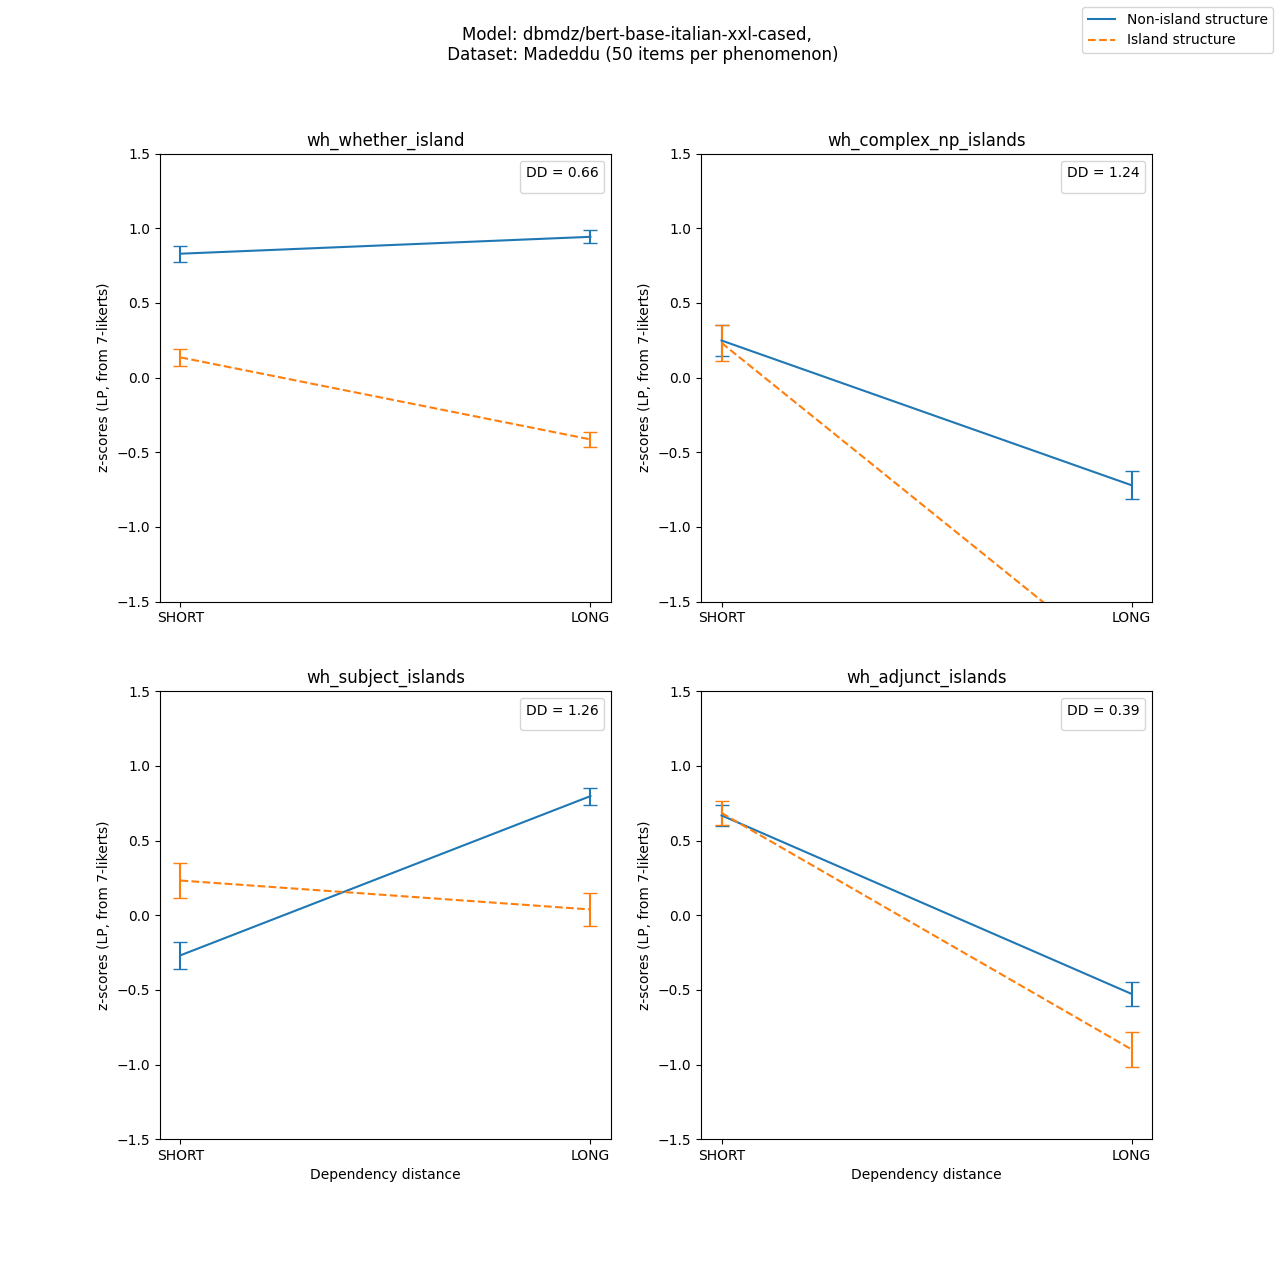
\includegraphics[width=1\textwidth]{images/Chapter1/Madeddu_wh_dbmdz_bert-base-italian-xxl-cased_LP-zscores-likert-2022-09-14_h15m39s52.png} 
	\caption{Plots of average acceptability scores from BERT XXL (13B of training tokens), on the test suites developed for the present thesis.}
	\label{fig:md_bert_lp} 
	\medskip
\end{figure}	

\begin{figure}[p]
	\centering
	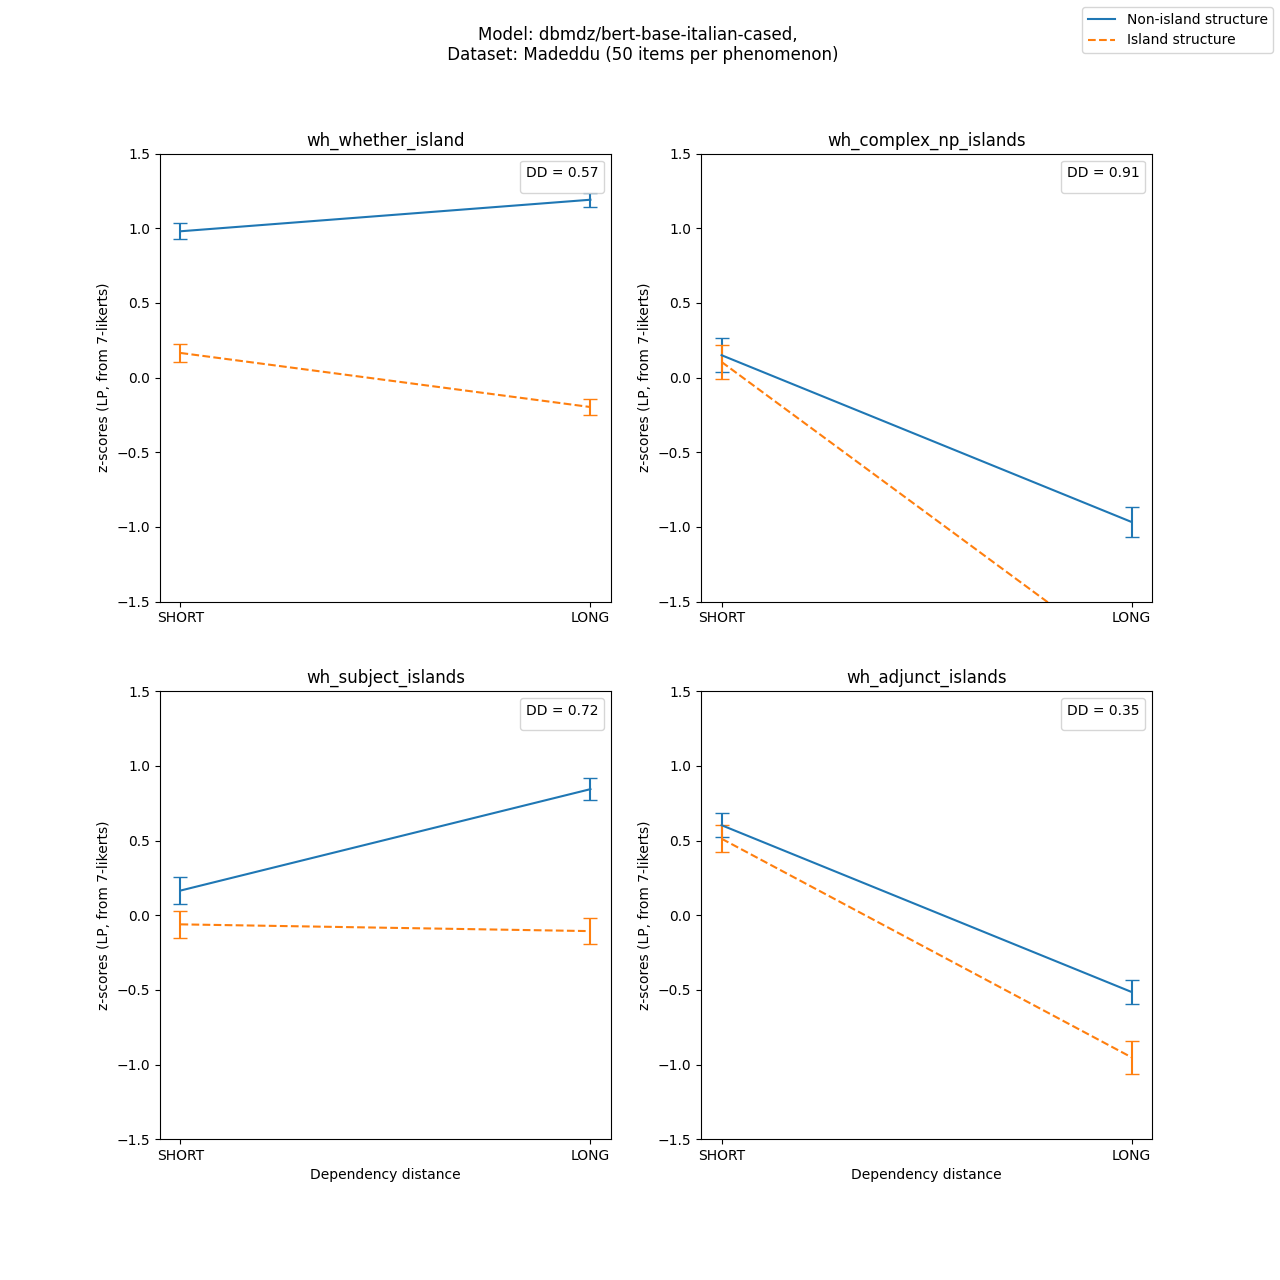
\includegraphics[width=1\textwidth]{images/Chapter1/Madeddu_wh_dbmdz_bert-base-italian-cased_LP-zscores-likert-2022-09-17_h11m10s08.png} 
	\caption{Plots of average acceptability scores from BERT (2B of training tokens), on the test suites developed for the present thesis.}
	\label{fig:md_bert2b_lp} 
	\medskip
\end{figure}	

% plots on Sprouse test suite

\begin{figure}[p]
	\centering
	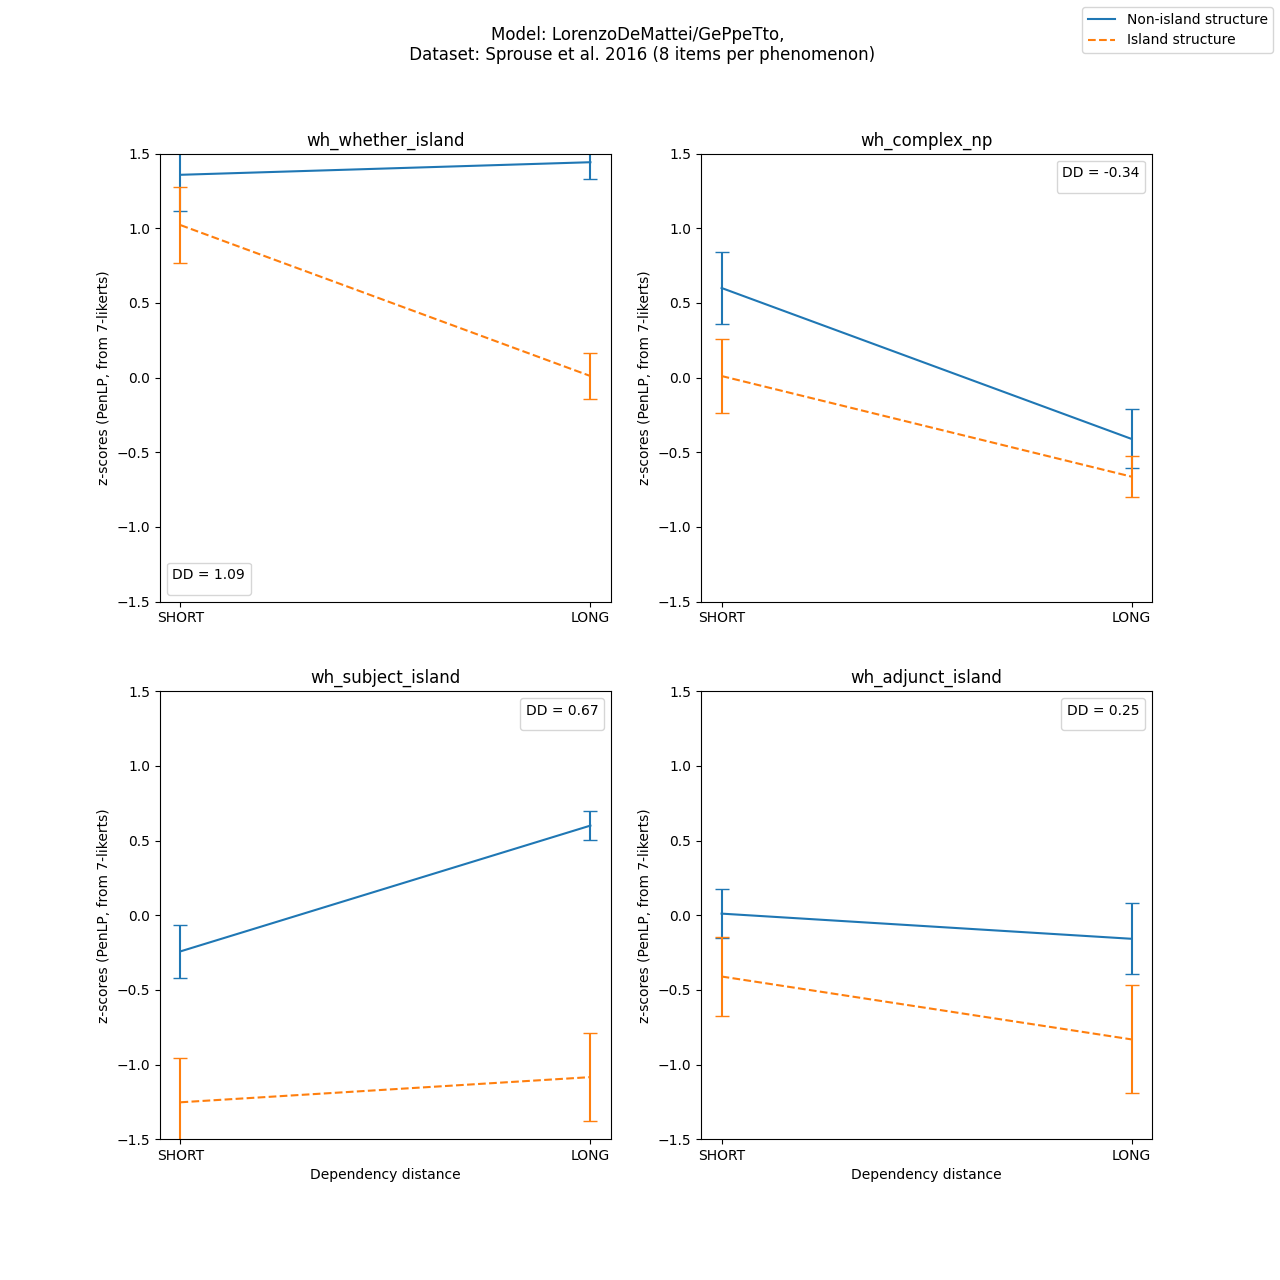
\includegraphics[width=1\textwidth]{images/Chapter1/Sprouse_wh_LorenzoDeMattei_GePpeTto_PenLP-zscores-likert-2022-09-14_h17m23s36.png} 
	\caption{Plots of average acceptability scores from GePpeTto, on the test suite by \citet{sprouse2016experimental}.}
	\label{fig:sprouse_gpt_penlp} 
	\medskip
\end{figure}	

\begin{figure}[p]
	\centering
	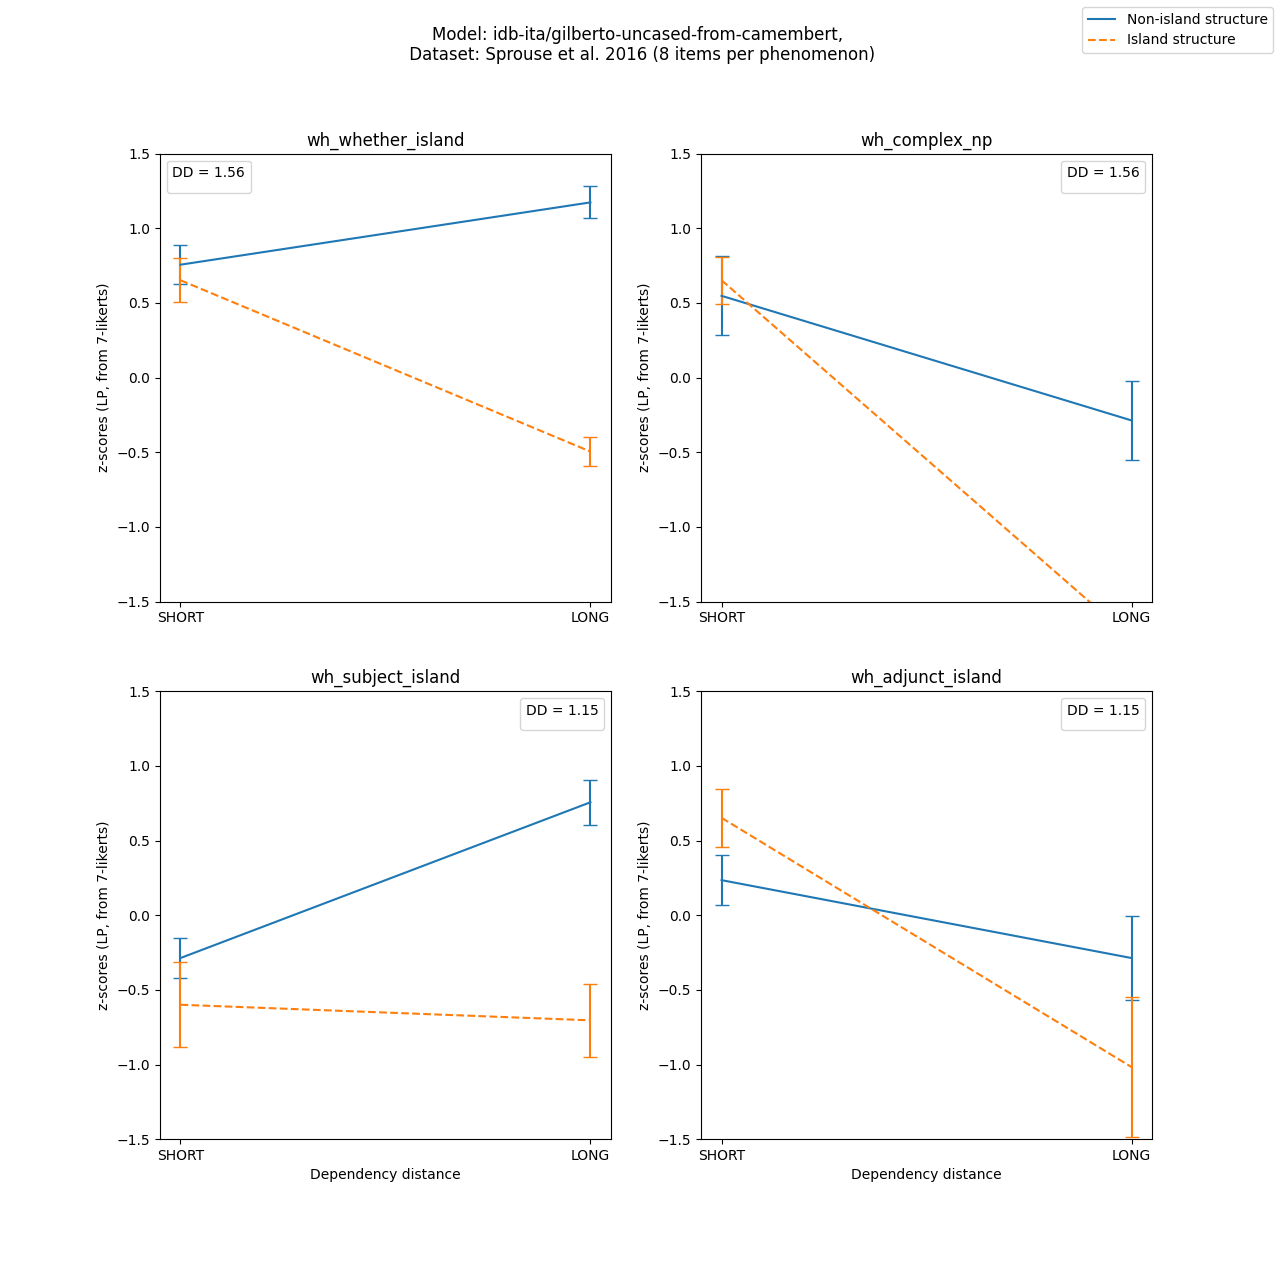
\includegraphics[width=1\textwidth]{images/Chapter1/Sprouse_wh_idb-ita_gilberto-uncased-from-camembert_LP-zscores-likert-2022-09-16_h10m19s47.png} 
	\caption{Plots of average acceptability scores from GilBERTo, on the test suite by \citet{sprouse2016experimental}.}
	\label{fig:sprouse_gilbertot_lp} 
	\medskip
\end{figure}	

\begin{figure}[p]
	\centering
	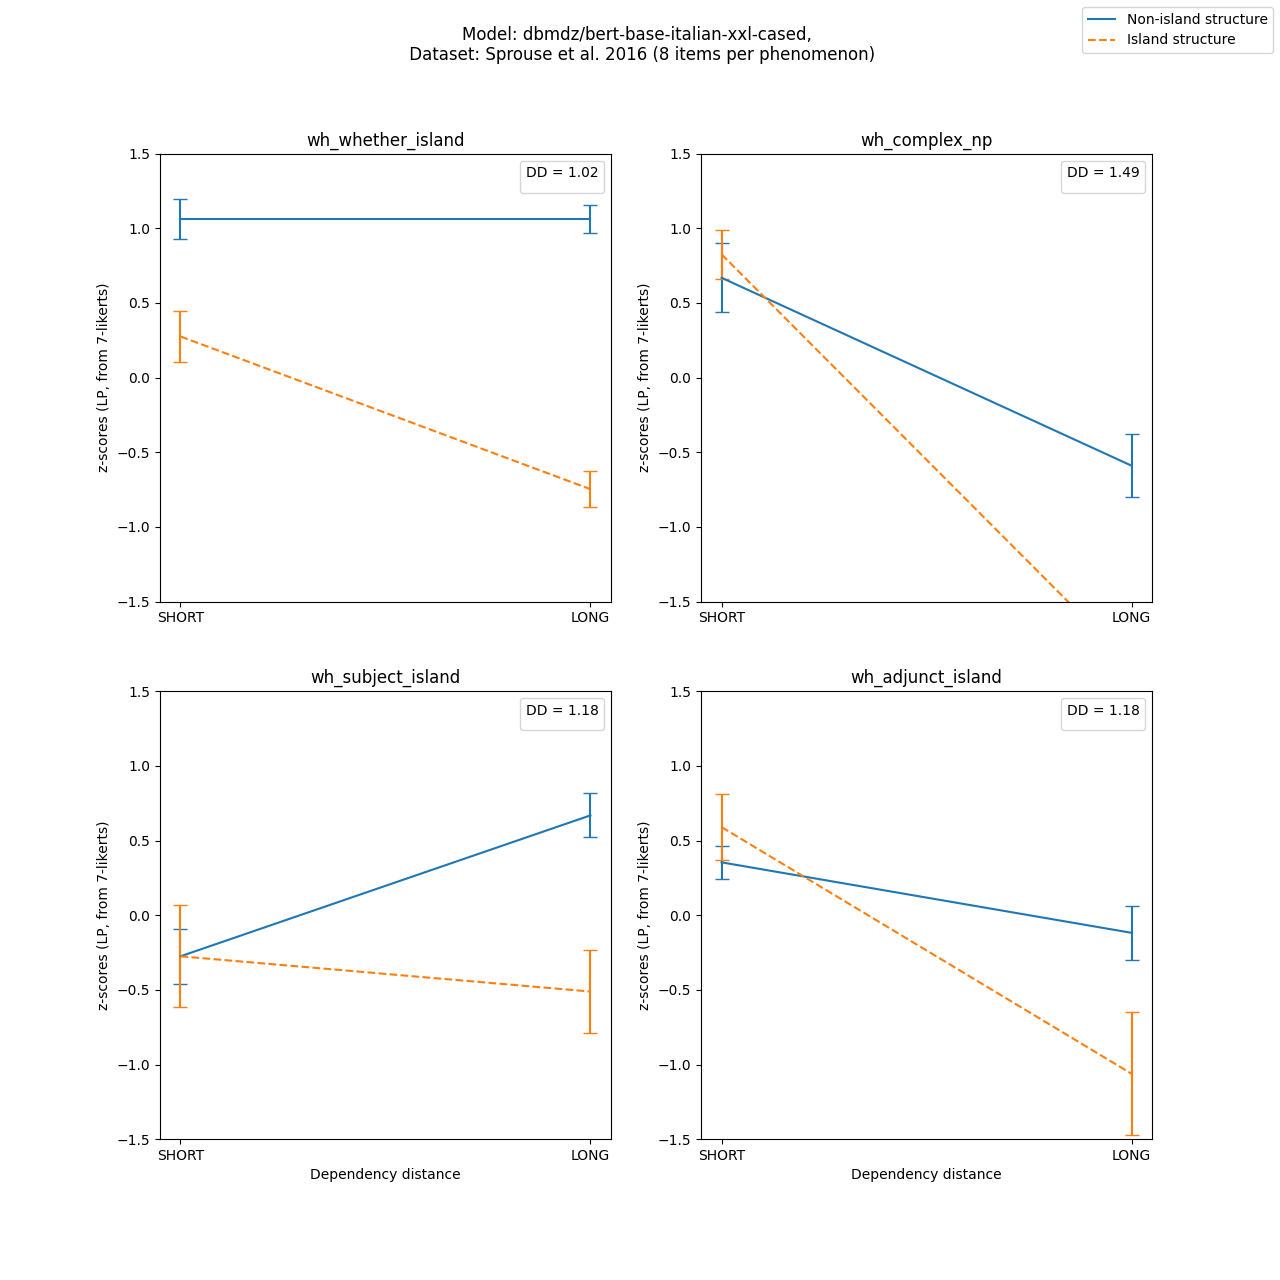
\includegraphics[width=1\textwidth]{images/Chapter1/Sprouse_wh_dbmdz_bert-base-italian-xxl-cased_LP-zscores-likert-2022-09-14_h17m27s24.png} 
	\caption{Plots of average acceptability scores from BERT XXL (13B of training tokens), on the test suite by \citet{sprouse2016experimental}.}
	\label{fig:sprouse_bert_lp} 
	\medskip
\end{figure}	

\begin{figure}[p]
	\centering
	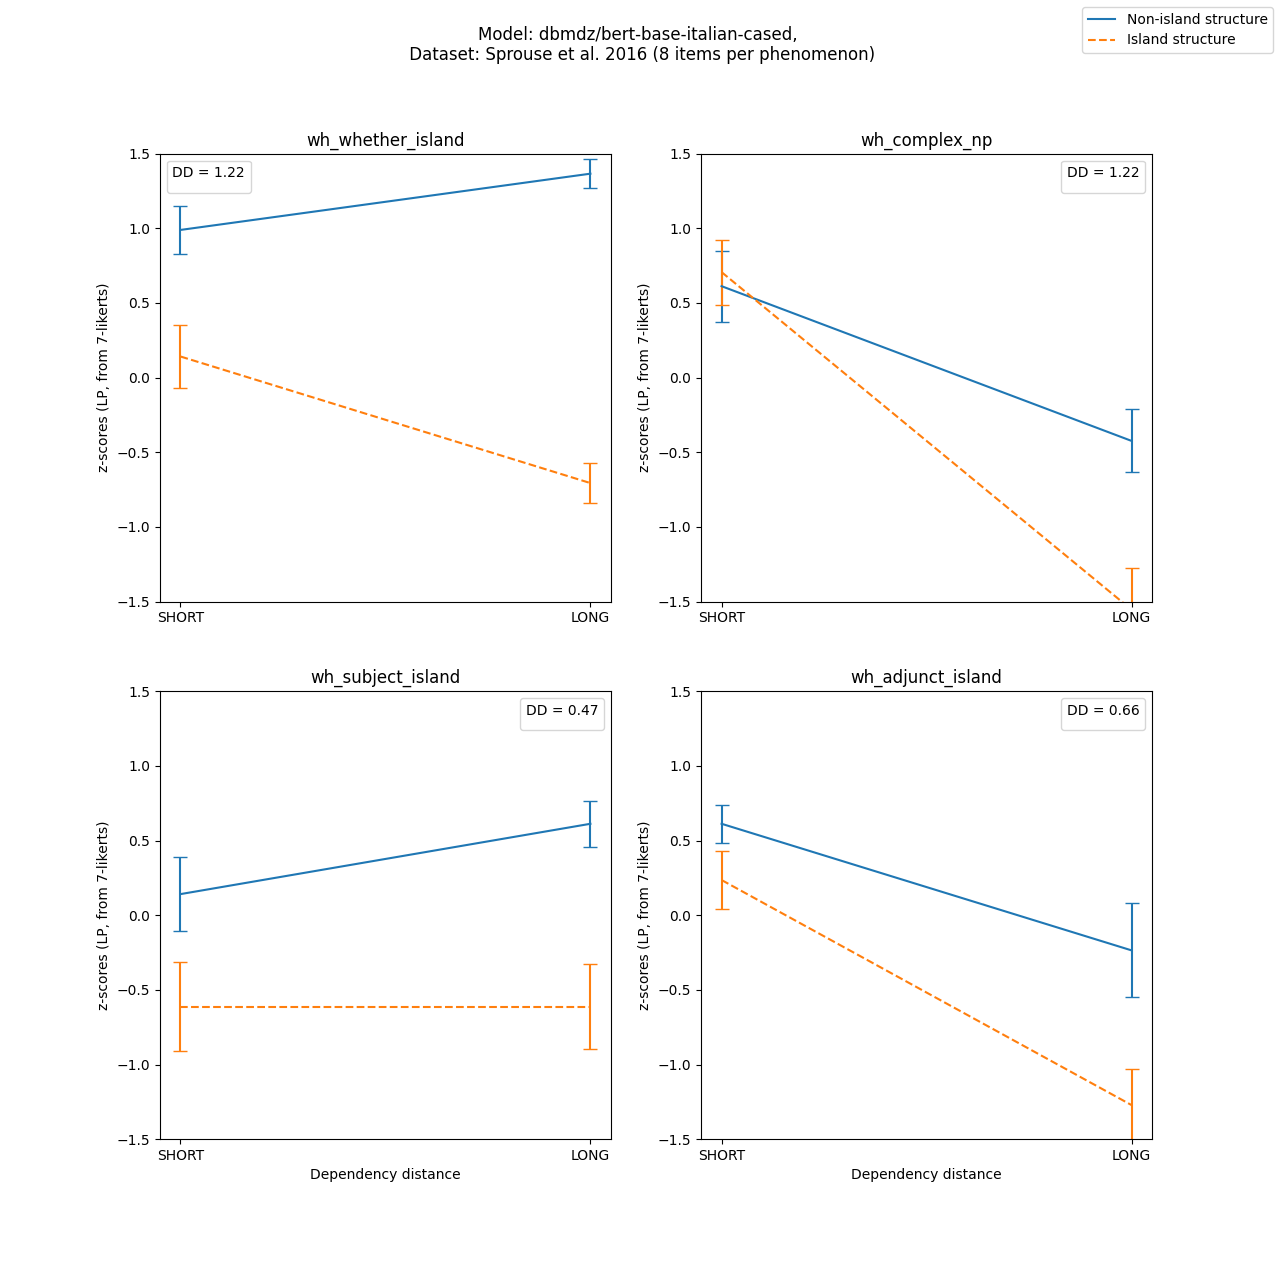
\includegraphics[width=1\textwidth]{images/Chapter1/Sprouse_wh_dbmdz_bert-base-italian-cased_LP-zscores-likert-2022-09-17_h11m04s37.png} 
	\caption{Plots of average acceptability scores from BERT (2B of training tokens), on the test suite by \citet{sprouse2016experimental}.}
	\label{fig:sprouse_bert2b_lp} 
	\medskip
\end{figure}	



\begin{figure}[p]
	\centering
	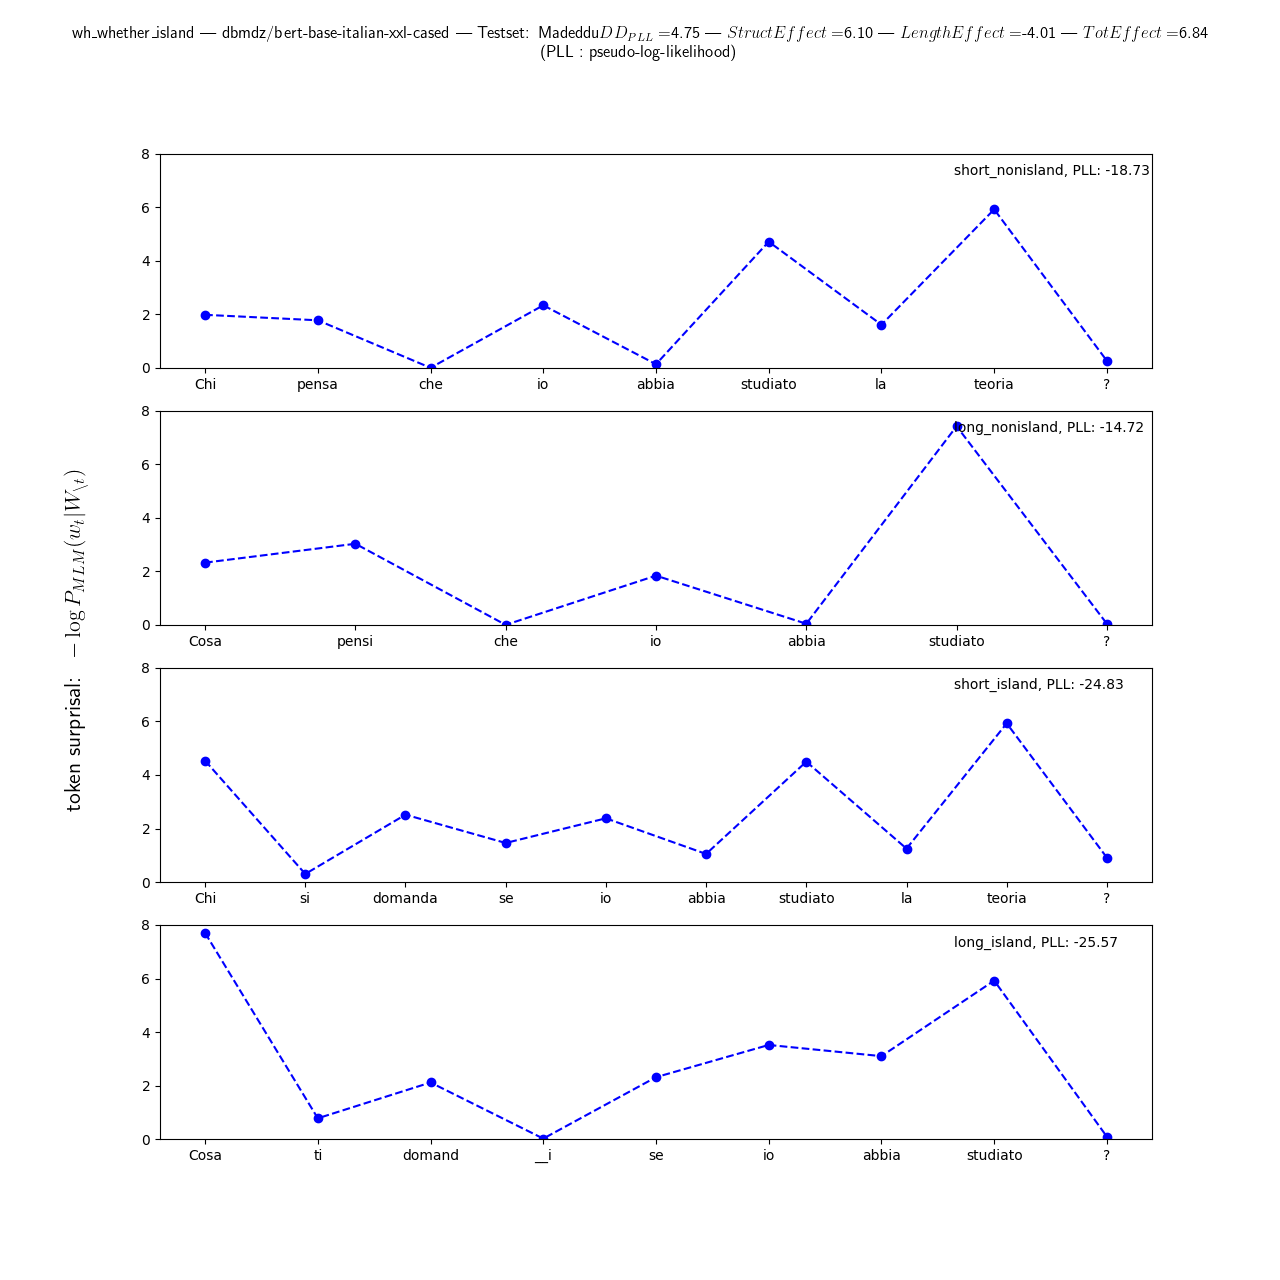
\includegraphics[width=1\textwidth]{images/Chapter1/token_surpisals/Madeddu_dbmdz_bert-base-italian-xxl-cased_wh_whether_island_item_158.png} 
	\caption{Token surprisal for the four sentences of one of the whether island items, as scored by the Italian BERT XXL.} 
	\label{fig:md_bert_whether_item_158_surprisals} % this internally labels the figure for future referencing.
	\medskip
	\small
	Token surprisal plots like this are a kind of "zoom" into the sentence acceptability estimates, since, in the case of BERT-based models, the sentence score is just the (negative) sum of the token surprisals. At the top of the figure there is the factorial DD score on the whole item (one that is $>0$ the item is considered scored accurately). There are also the factorial measures of length and structure effect, and the total effect. Note that these are raw values obtained from the (negative) sum of the token surprisals, while the values seen in plots like in \autoref{fig:md_gilberto_lp} are normalized across all the sentence scores for all the phenomena given by a particular model.
\end{figure}

\begin{figure}[p]
	\centering
	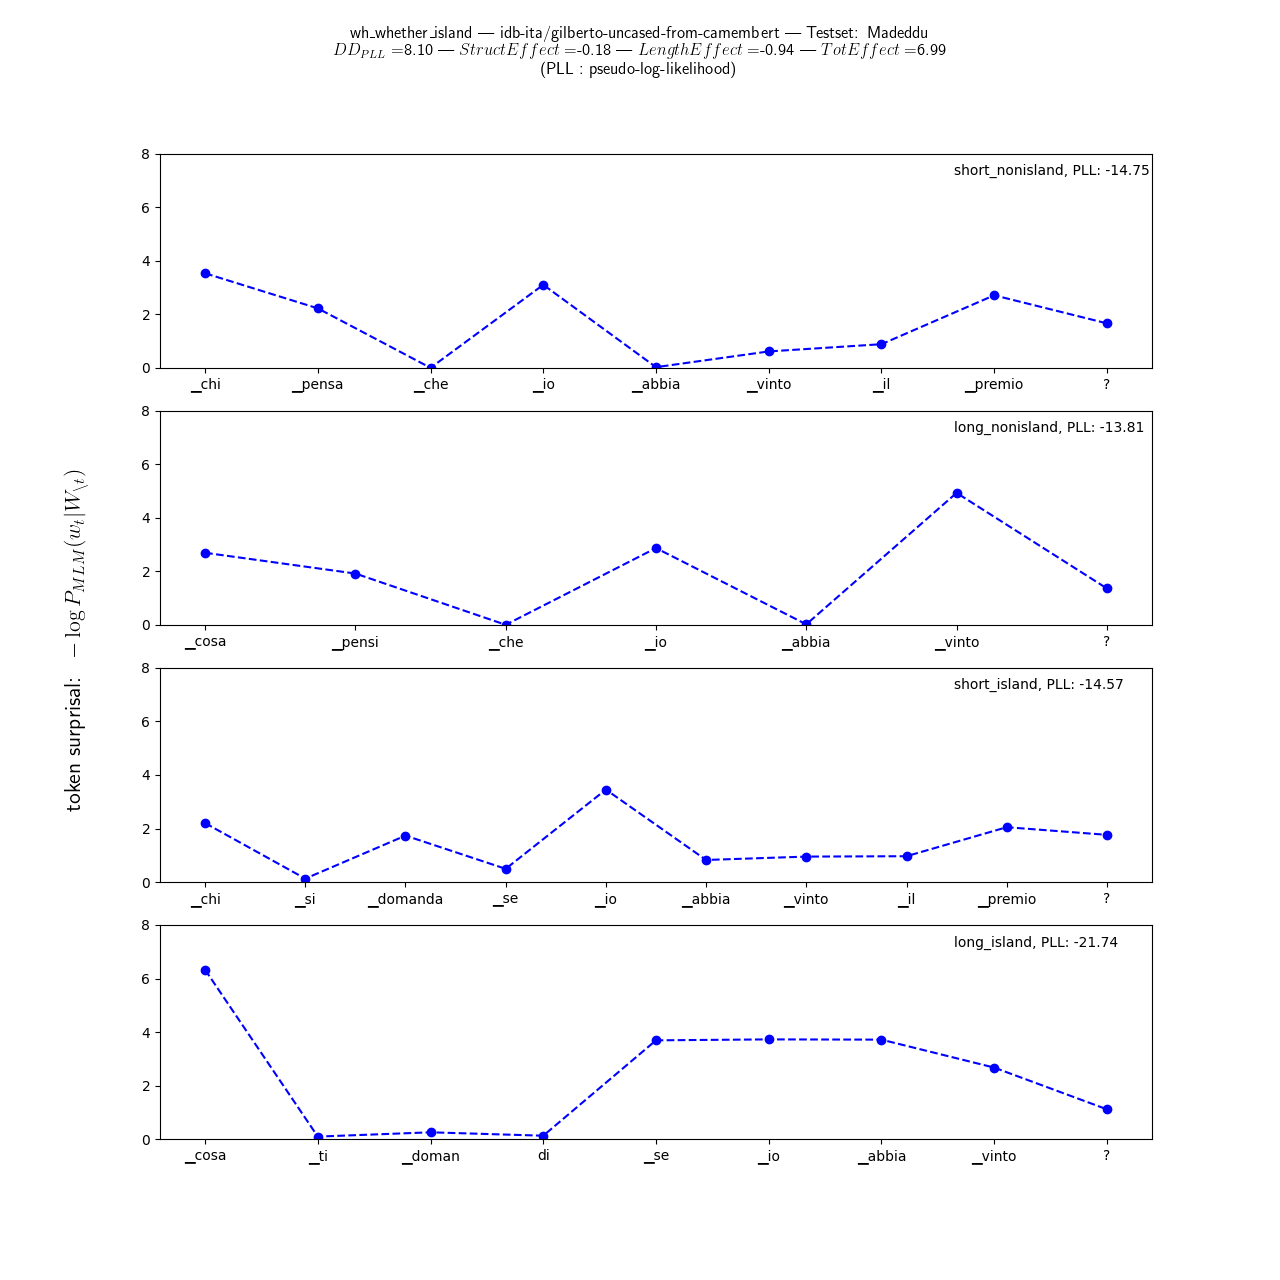
\includegraphics[width=1\textwidth]{images/Chapter1/token_surpisals/Madeddu_idb-ita_gilberto-uncased-from-camembert_wh_whether_island_item_152.png} 
	\caption{Token surprisal for the four sentences of one of the whether island items, as scored by GilBERTo.} 
	\label{fig:md_gilberto_whether_item_152_surprisals} 
	\medskip
	\small
	Note that the tokens are lowercased because GilBERTo is available only in the uncased version, otherwise uppercase words would be split, increase the surprisals, and introduce confounds.
\end{figure}

\begin{figure}[p]
	\centering
	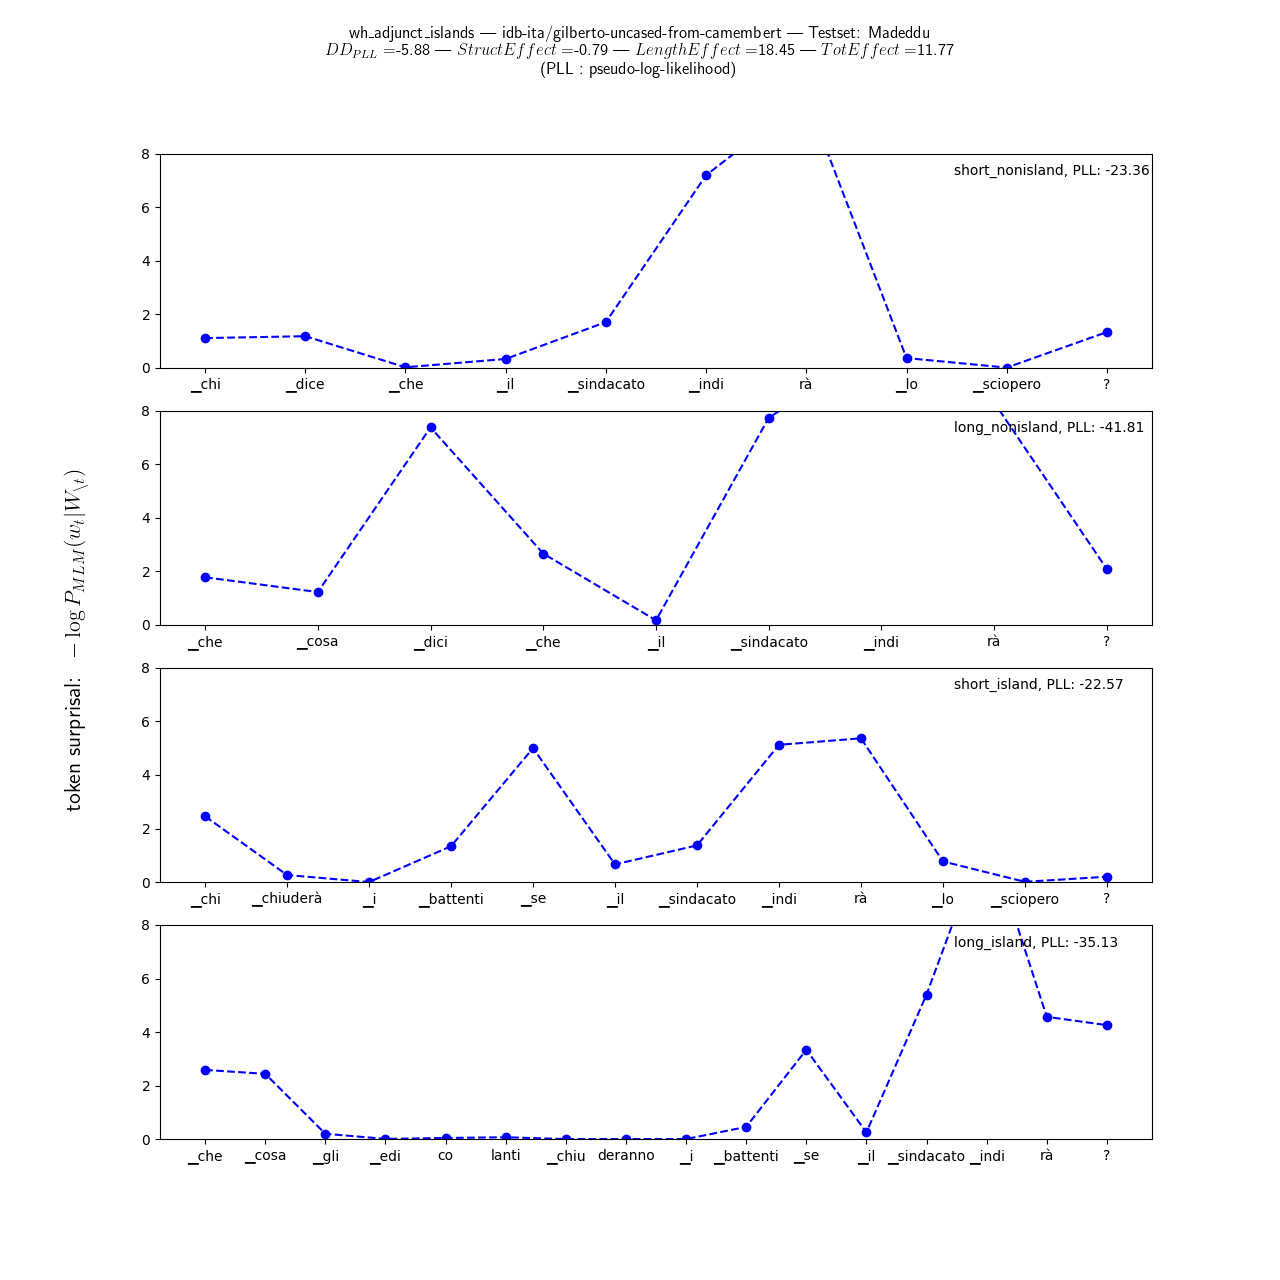
\includegraphics[width=1\textwidth]{images/Chapter1/token_surpisals/Madeddu_idb-ita_gilberto-uncased-from-camembert_wh_adjunct_islands_item_195.png} 
	\caption{Token surprisal for the four sentences of one of the adjunct island items, as scored by GilBERTo.} 
	\label{fig:md_gilberto_adjunct_item_195_surprisals} 
	\medskip
	\small
\end{figure}


\subsection{Whether islands}
One difference is that for whether islands (for GPT-2 but also for the other two language models, \autoref{fig:md_gpt_penlp}-\autoref{fig:md_gilberto_lp}), the line connecting the \textsc{short-nonisland} and the \textsc{long-nonisland} goes upwards instead of downwards like for humans; that is, on average the language models give the \textsc{long-nonisland} a higher acceptability estimation score (the pseudo-log-likelihood, PLL), than the \textsc{short-nonisland} (and this trend remains also when the models score the original test suite administerd by Sprouse to humans, diplayed in \autoref{fig:sprouse_gpt_penlp}-\autoref{fig:sprouse_bert2b_lp}).

To explain why, we can have a look at \autoref{fig:md_bert_whether_item_158_surprisals}, which shows the surprisals of each token in one of the whether islands items. The token surprisal plots like this are a kind of "zoom" into the sentence acceptability estimates, since, in the case of BERT-based models, the sentence score is just the (negative) sum of the token surprisals. 

In \autoref{fig:md_bert_whether_item_158_surprisals}, we see that the \textsc{short-nonisland} sentence ("\textit{Chi pensa che io abbia studiato la teoria?}") has the additional tokens "\textit{la teoria}", which significantly adds to the total sum of surprisal. The same phenomenon can be see in \autoref{fig:md_gilberto_whether_item_152_surprisals}, where the phrase "\textit{vinto il premio}" (found in the \textsc{short-nonisland}) sums up to slightly more surprisal than the word "\textit{vinto}" alone (found in the \textsc{long-nonisland}). However, in general we can't just assume that a longer sentence will get a lower acceptability scores, because having more content words can give more semantic cues, making it easier to predict each of them when it's masked during the scoring, lowering the surprisals (as can be seen in \autoref{fig:md_gilberto_adjunct_item_195_surprisals}, discussed in the next paragraph).

% ..

% \subsubsection{Whether islands}

%From \autoref{fig:wh_whether} for whether islands with wh-dependencies, we can see that the GTP-2 model, compared with the results from humans gives higher (more acceptable) scores for all sentence types. This difference is more pronounced in the scores performed by Gpt on the original test suite from \citet{sprouse2016experimental} (middle image). 
% note at the beggining of plots: note that these scores cannot really be used in the aboslute.. but showa a relative trend among island types, with correspondence with humand score. For instance, sentences in items testing .. islands tend to score highest, while .. around middle, and .. lowest.

%The slope of the lines (both for island and non-island sentence structures) is however similar to the human scores. \\


%\begin{figure}[H]
%	\centering
%	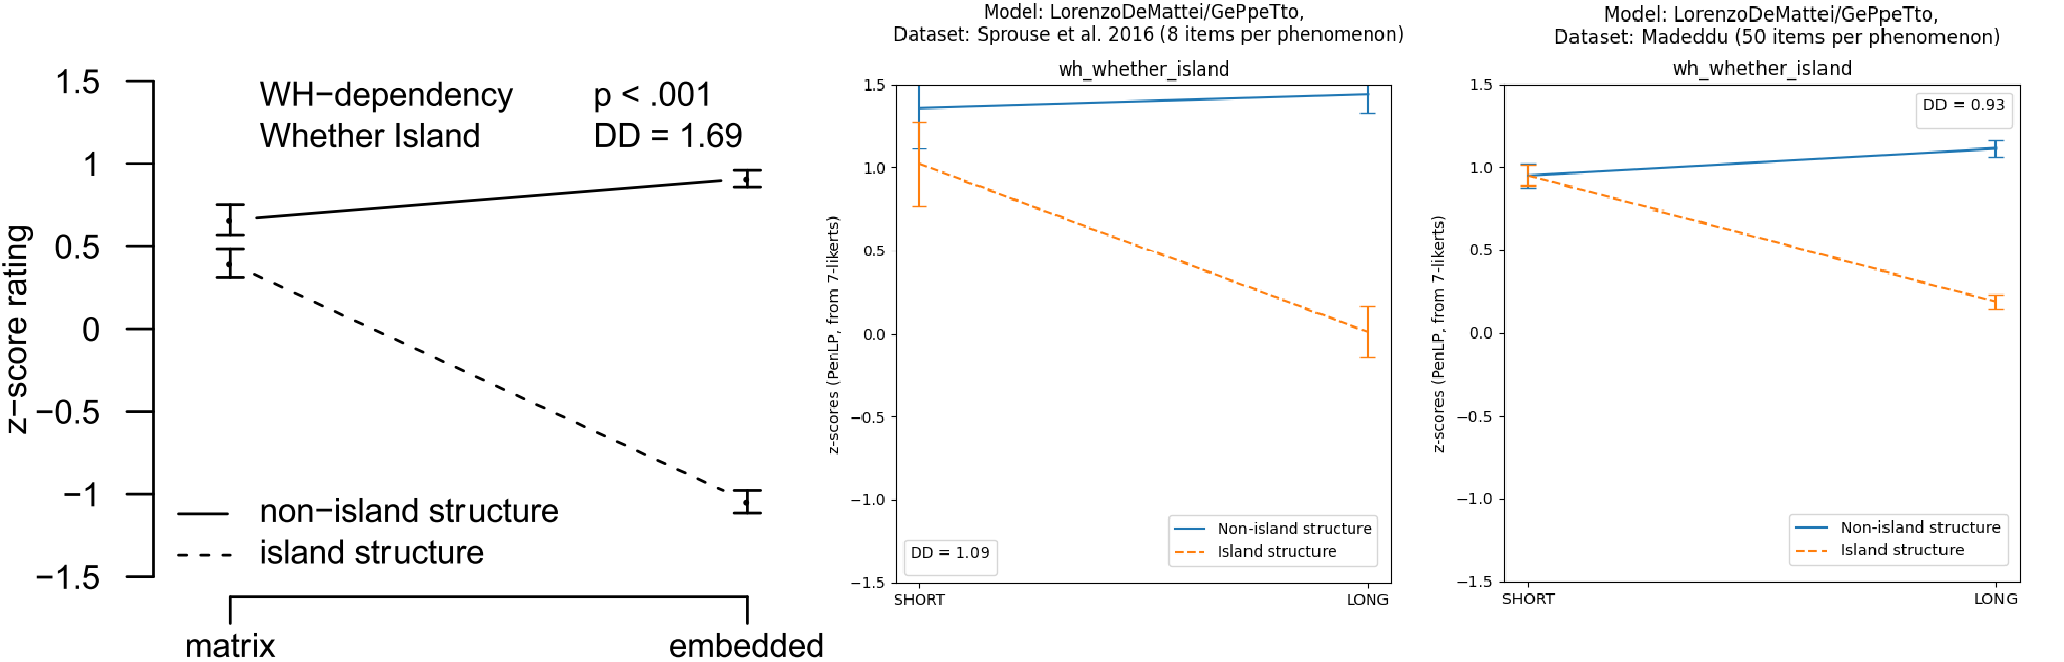
\includegraphics[width=1\textwidth]{images/Chapter1/combined_wh-whether.png} % width= 0.8\textwidth
%	\caption{Comparison of wh-dependency whether islands} 
%	\label{fig:wh_whether} % this internally labels the figure for future referencing.
%\end{figure}


% TODO: table showing accuracy scores for the 4 sentences of an item; comparison on variations across multiple items


\subsection{Adjunct islands}
GilBERTo has a much lower accuracy score (72\%) than GPT-2 (98\%) for adjunct islands (\autoref{tab:accuracy_DD_it_data}), and this is the only island type in which it doesn't outperforms or at least come very close to both of the other two models. From the plots it seems that this is due to the \textsc{long-nonisland} sentences getting on average too low of an acceptability, so the expected \textsc{length-effect} that will be subtracted from the total effect (formula \ref{formula:factorial_score}) is really large (\autoref{fig:md_gilberto_lp}). 

Looking at the token surprisal for one of the items (of a conditional island construct introduced by "\textit{se}"), we can see in \autoref{fig:md_gilberto_adjunct_item_195_surprisals} that the \textsc{long-nonisland} (second sentence from the top) gets really high spikes for the phrase "\textit{il sindacato indirà}" ("\textit{the union will call}"), while in the case of the \textsc{short-nonisland} (first sentence from the top), the phrase "\textit{il sindacato indirà lo sciopero}" ("\textit{the union will call the strike}") gets a much smaller surprisal on the word \textit{sindacato} ("\textit{union}"), seemingly because the presence addition of the word for \textit{strike} (which, mutually, also gets almost no surprisal for the same reason) makes it much more likely to predict when masked. However, these spikes are also present (albeit a bit ameliorated) in the \textsc{long-island} sentence (last at the bottom), so this effect would be subtracted out by the factorial scoring. The thing that keeps the DD score negative (and therefore renders this item inaccuratly scored) is that the \textsc{long-nonisland} sentence has also a surprisal spikes for the phrase "\textit{dici che}" ("\textit{you say that}"), and this seem to be due to syntactic reasons: the model seems to consider less likely this kind of long-distance dependency construct ("\textit{che cosa dici che il sindacato indirà?}") than another long-distance dependency construct where there is a island violation ("\textit{che cosa gli edicolanti chiuderanno i battenti se il sindacator indirà?}"). We can conclude then that the worse accuracy score that GilBERTo gets in adjuncts islands (\autoref{tab:accuracy_DD_it_data}) seems to be indeed due to an \textbf{unrobust learning of this type of adjunct island constraints} by GilBERTo.

Also in \autoref{fig:md_gilberto_adjunct_item_195_surprisals} (an adjunct island item scored by GilBERTo), we can notice what seems to be causing the \textsc{short-island} sentences to have a higher acceptability estimate than \textsc{short-nonisland} ones, and therefore the island and non island lines to "cross" in \autoref{fig:md_gilberto_lp} (plot at the bottom-right). The \textsc{short-nonisland} too has the phrase "\textit{il sindacato indirà lo sciopero}", but it has also additional content words that give semantic cues and therefore further lower the surprisals, with the phrase "\textit{chiuderà i battenti}".

GPT-2 seem to have learned adjunct island constraints more robustly than the two BERT-based models, as mentioned above. Looking at \autoref{fig:md_gpt_penlp} it seems this is due to the higher gap in acceptability given by GPT-2 than BERT and GilBERTo (\autoref{fig:md_gilberto_lp}). In the case of GPT-2, the gap it's almost 1 standard deviation (these are normalized z-scores), while it's about half that for the BERT-based modes (\autoref{fig:md_gilberto_lp}).
% todo: add code to show the per token scores from Gpt2, and then generate the spikes plots

% Chi dice che lo studente avrebbe studiato la teoria (and following examples)
%In Fig. (item 197 for GilBERTo and adjunct islands) we see that there is probably a confound due the use of the less common verb form "\textit{avrebbe studiato}" ("he had studied", subjunctive mood) in the sentences with a non-island structure (two top plots), while in the sentences with an island structure (two bottom plots) there is the more common form "\textit{aver studiato}" ("having studied", infinitive).
% Balancing variant "ha studiato"; it could be used also in the island sentences with a relative "che ha studiato"

%\subsubsection{Adjunct islands}
%
%\begin{figure}[H]
%	\centering
%	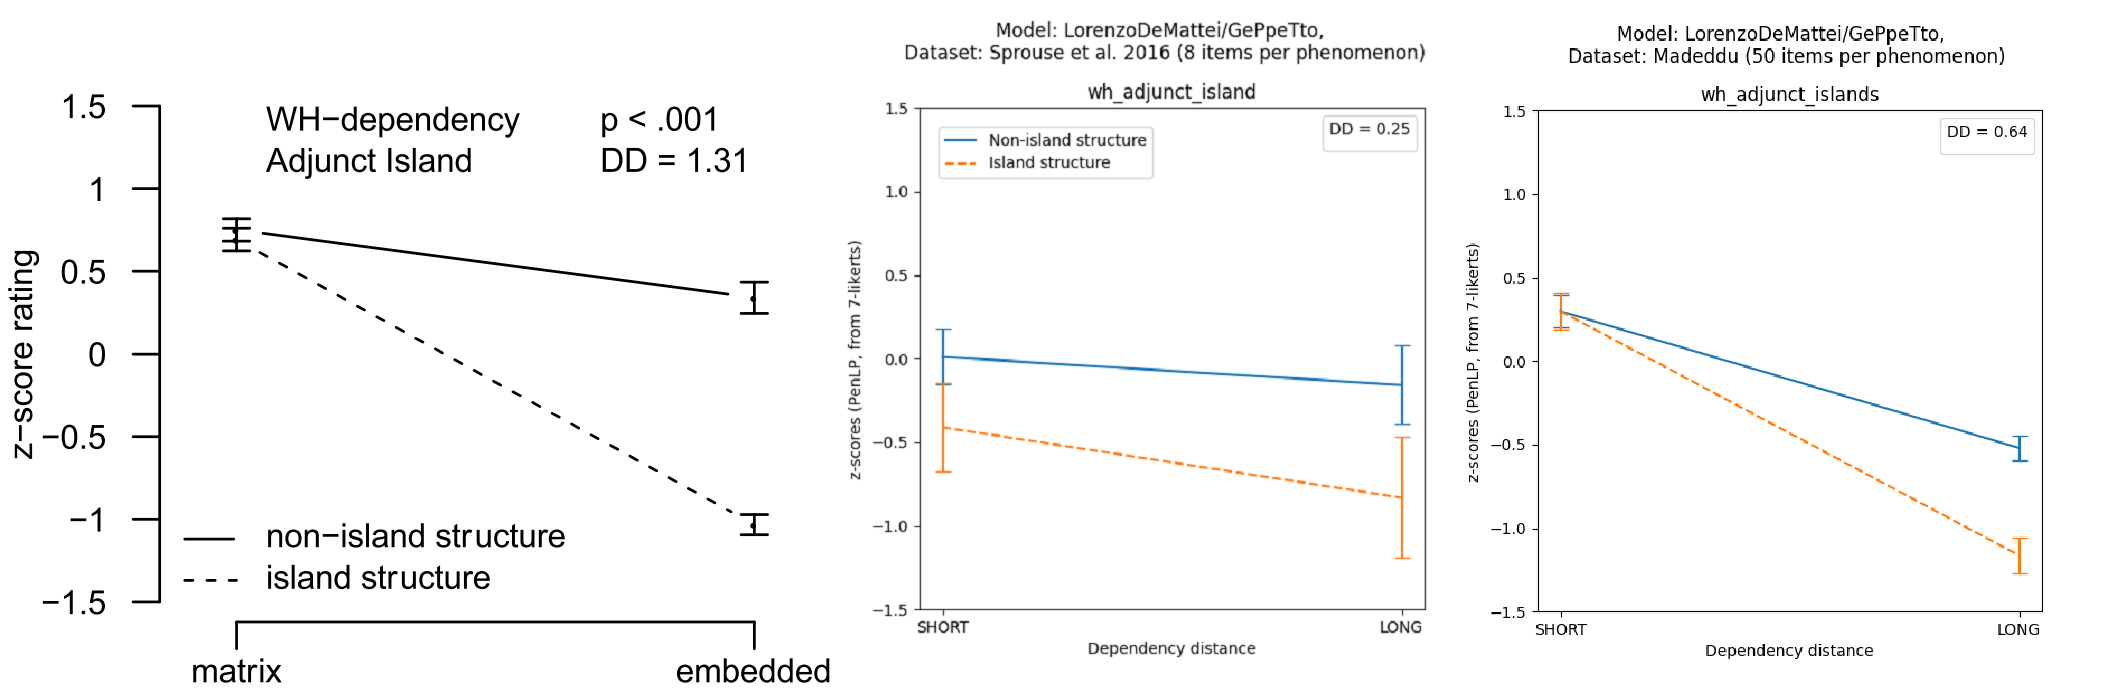
\includegraphics[width=1\textwidth]{images/Chapter1/combined_wh-adjunct.png} 
%	\caption{Comparison of wh-dependencies adjunct islands} 
%	\label{fig:wh_adjunct} % this internally labels the figure for future referencing.
%\end{figure}
%
%
%In \autoref{fig:wh_adjunct} the slope of both lines on the new test suite (right image) is similar to the human scores (left image), althoughg with a lower average acceptability for the Long-NonIsland sentences, which results in a downward steeper line. 
%
%In the test suite we developed for this thesis, the Long-Island sentences for adjunct islands have a form that might make them more easily identifiable has unacceptable than the ones in the Sprouse test suite: compare \textit{Che cosa Gianni è partito per Parigi dopo aver fatto?} (\textit{What did Gianni left for Paris after doing?}) in the new dataset, with \textit{Cosa ti irriti se dimentico in ufficio?} (\textit{What do you get irritated if I leave in the office?}) in the original test suite by Sprouse. The ending of the first sentence with a gap might be less frequent and result in a lower acceptability score. 
% in the sprouse data, at the end there is a preprositional ..phrase like “in ufficio”.

\subsection{Complex NP islands}
Conversely from the adjuncts islands, GPT-2 seems to struggle with complex NP islands (46\% accuracy in \autoref{tab:accuracy_DD_it_data}), compared to BERT (100\% accuracy) and GilBERTo (98\% accuracy). This is also reflected in the factorial plots showing the average sentence acceptability scores: the one for BERT (\autoref{fig:md_bert_lp}) and GilBERTo (\autoref{fig:md_gilberto_lp}) have slopes similar to the plots from human scores (\autoref{fig:sprouse_humans}), while GPT-2 stands out as different (\autoref{fig:md_gpt_penlp}).


% effect of more training data, from bert to gilberto, increases in accuracy
% discuss differences: ..
% then note: this improvement from bert to gilberto reflects the low sample efficiency of these models, and/or the current way of training them (e.g. in a text-only single modality): they still require more than .. B tokens to learn more advanced syntactic phenomena like island effects.
% note: more challeging tests might be needed for the other phenomena too, to account for ..frequency effects of constructs, vocabulary..

%In the middle and right images on \autoref{fig:wh_complex}, we see that, for complex NP items, the long non-island sentences (blue line, right edge) on average get scored by the GPT-2 model with a lower acceptability than by the human subjects, shown in the left image. 

% (\autoref{fig:md_gpt_penlp}) BERT XXL (\autoref{fig:md_bert_lp}) \ref{fig:md_gilberto_lp}

We see that, for complex NP items (top-right plot of each figure from \autoref{fig:sprouse_humans} to \autoref{fig:md_bert2b_lp}), the long non-island sentences scored by the GPT-2 model with a lower acceptability than by the human subjects, and on the right edge the blue line and orange line converge to the same low value. This does not happen in the BERT XXL  (\autoref{fig:md_bert_lp}) and GilBERTo models (\ref{fig:md_gilberto_lp}). This might be due to the GPT-2 model being more sensitive to more marginal sentences ending with a gap followed by a question mark, as in the long-distance dependency sentences tested for this type of island ("\textit{Che cosa pensi che Gianni avrebbe comprato \_?}", en: "\textit{What do you think Gianni has bought?}").
%This seems to be due to the long distance dependency effect, that gets exacerbated as a sentence increases in lenght (in these test suites, the complex NP islands examples have longer sentences).

%\begin{figure}[H]
%	\centering
%	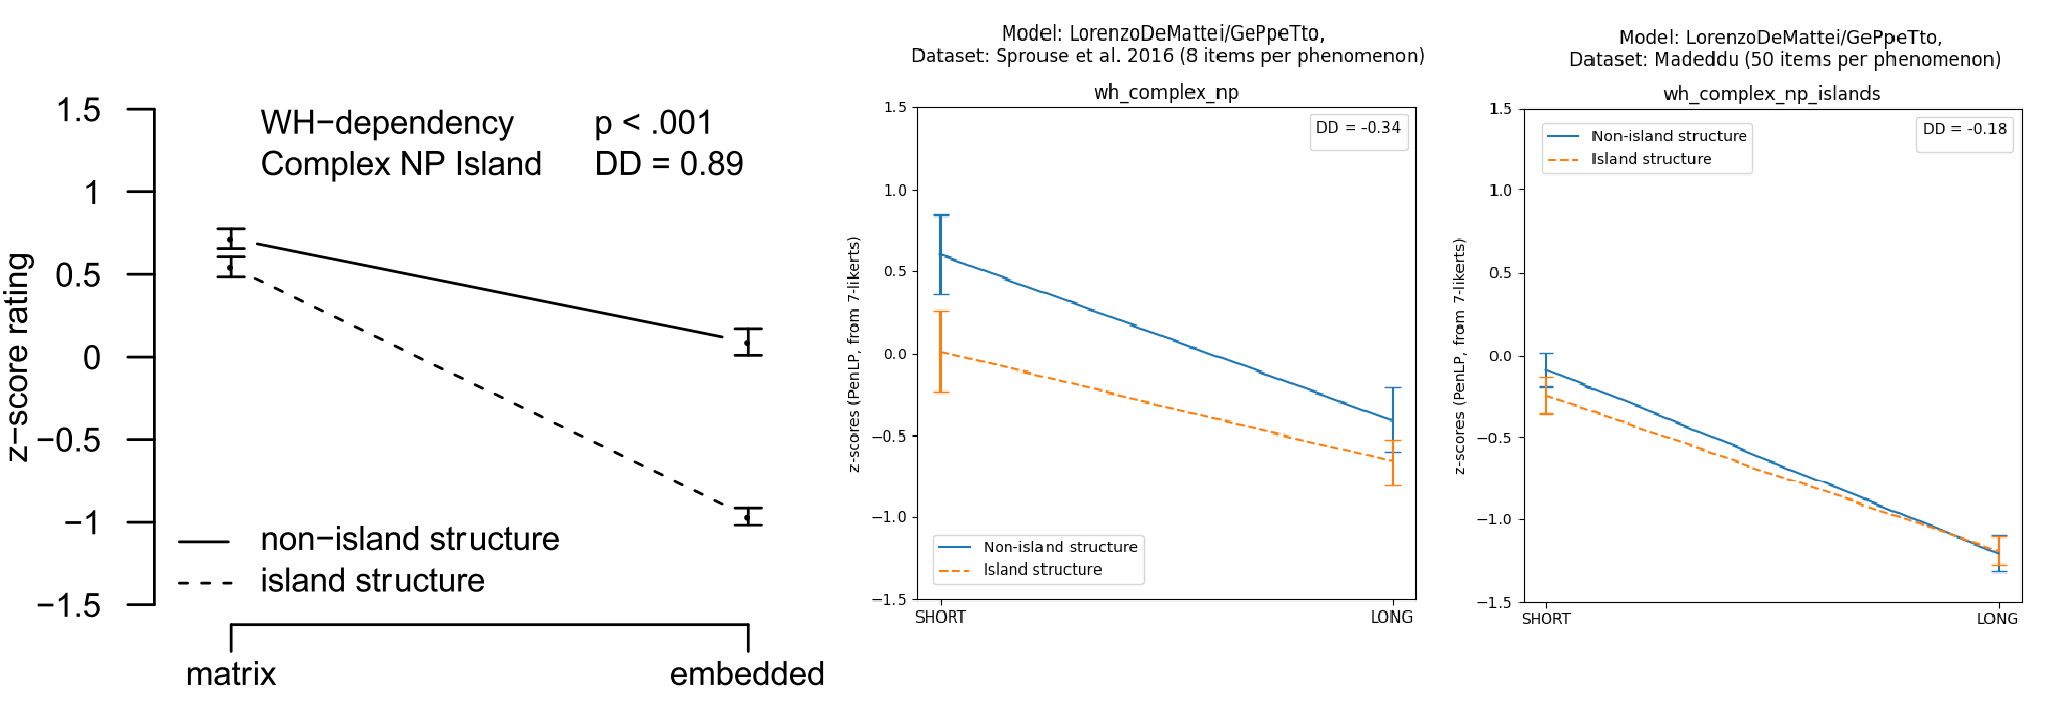
\includegraphics[width=1\textwidth]{images/Chapter1/combined_wh-complex.png} 
%	\caption{Comparison of plots for wh-dependencies complex NP islands} 
%	\label{fig:wh_complex} % this internally labels the figure for future referencing.
%	\medskip
%	\small
%	The first plot on the left shows the scores on humans subjects published in \citet{sprouse2016experimental} for Italian complex NP islands with wh-dependencies. For each line, the left-most edge represents the score for the short-distance dependency sentence, the right-most the long-distance dependency. The plot in the middle shows the scores from a Gpt-2 model \citep{de2020geppetto} on the same test suite used for the first plot. The plot on the right shows the scores from the same Gpt-2 model but on the expanded test suite developed for the present thesis.
%\end{figure}

% still the problem overall in the orginal plots seems an overly low score for the long non island sentences
% that is, is the long distance depencency that receives a too loo score .. (lenght effect?)
% while the structure effect ..
% albeit it's correct, like humans scores, that the long non island has less acceptability than the short island
% then how is the long distance dependency (lenght effect) scored for the other island phenomena?
% the difference with the sentences for the other phenomena seem to be that they have a simpler main clause, like "cosa pensi che" (present) + "abbia ppt"  (congiuntivo passato), while for the complex np, is "cosa hai smentito/annunciato/raccontato/sostenuto che" (passato prossimo) + "avrebbe ppt" (condizionale passato)
% a comparison example could be to turn the other 3 island phenomena items into passato prossimo for the main clause
% but was this discrepancy also in Sprouse data, and is this the reason for their plots differences too? (so the gpt2 model just accentuates this drop in acceptability?)


\subsection{Subject islands}
Comparing the plots from BERT XXL (\autoref{fig:md_bert_lp}) with those on humans (\autoref{fig:sprouse_humans}), we can see that the in the BERT XXL plot for subject islands, the two lines cross, unlike in those for humans. This is due to the fact that BERT XXL (on average) scores with very low acceptability the simplest sentence (the one for the \textsc{short-nonisland} condition on), lower than the other three sentence conditions. So the variation from it to any of the other three sentences sees and increase in acceptability. But the overall DD score is still positive (hence the 90\% accuracy BERT XXL gets on this island type, albeit less then the 94\% by GilBERTo), because the increase in acceptability from \textsc{short-nonisland} to \textsc{long-island} (a-d in formula \ref{formula:factorial_score}) is still lower than the increase expected from the sum of the two other factors (length and structure), therefore this less-than-expected increase can be attributed to a super-additive island effect.
% but ideally we should revise the items to avoid this effects, less confounds to subtract out, more clear effects

% GPT-2, despite having a plot for subject islands very similar to that of humans, unlike GilBERTo, and expecially BERT, these both overperform it in the accuracy score. ..(82, 90, 94)



% (also likely ngram sequences lower the surprisal)

% list of things to check with the spikes analysis: ..

% on GPT, but in BERT the trend is similar as on humans, just with all scores shifted downawrds. Regarding this, it's word rememberinght what ..discussed in section .., about the fact that the acceptability scores are not really comparable in absolute, but only relatively within minimal varying pairs or items. Therefore, plotting the values aggregating the scores, even with a ..likert notmalization and ..minus mean normalization, it's still a ..forzatura.
% todo but add note that initially, from the "promising" paper of lau et al 2017, this measures seemed to be used as absolute acceptability measure directly from pretrained models.. so they someout work, but are ..very prone to confounds..
% so that's why the minimal pairs approach seems to be better, although it's tricky to design minimal pairs/items ("miminal items"/"minimal factorial items" approach, a generalization of the minimal pairs one. BLiMP, benchmarck of linguistic minimal ..items)

% modified design for subject islands as in Sprouse 2016: "the non-parallel lines have slopes in opposite directions"
% "the implicit control afforded by the factorial design that was mentioned in Sect. 3. " (Sprouse 2016)


%Comparing the plots from BERT with those on humans, we can see again the discrepancy with the \textsc{short-island} sentence of the adjunct island (likely due to the confound discussed above).
%Bert seems to score the complex NP islands better than GPT2, with plots that resemble more those from humans.
%
%For subject island (that have ..a modified factorial design as discussed in section ..) we see that BERT scores higher the \textsc{short-island} sentence than the \textsc{short-nonisland}, contrary to what happens with humans and with GPT2. To better explain why we should have a look at the spike analysis in the following section. In any case, this effect seems to be subtracted out by the factorial score, so BERT still gets the best accuracy score for this type of island as seen in table ..

%
%The Gpt-2 scores on the original Sprouse et al. test suite (middle image) have wider standard error bars, which are considerably smaller for the new test suite developed for the present thesis (right image).\footnote{This might be due to the fact that the number of items between the two test suites increases from 8 to 50.}
%in fig .. (Sprouse test suites, language models), we see that the ..error bars (..confidence intervals?) are wider, and this is probably due to the fact that the sample sizes are smaller (8 items per phenomenon instead of 50), so there is probably more variance.

%While on human ratings the unacceptable sentences (Long-NonIslands) receive all on average a z-score of about -1, there is more variability in the scores given by the Gpt model, in particular for whether islands sentences (\autoref{fig:wh_whether}), which receive much higher acceptability rating on average (betwenn 0 and 0.5 the Sprouse test suite and ours).

% todo: gpt2 plots more similar to Sprouse plots from humans scores: this might be related to the finding by (..Venturi paper) that GPT2 scores are more interpretable than BERT ones..


% todo: regenerate Sprouse's plots from the published score data?


% Surprisal ( $\displaystyle\-log P_{MLM} (w_t | W_{\setminus t}) $)


% Fig.1 Results from Sprouse et al (2016)
% Fig.2 Results of acceptability judgements to the same stimuli from Sprouse et al. 2016 from an Italian Gpt-2 model (GePpeTto) with the PenLP acceptability ..score. 
% Fig.3


% gpt2 token spikes analysis:
% - use to demonstrate the reason for GePpeTto accuracy scores/plots
% use to obtain a plot for numerical analysis comparison of output (descending curve for gpt, "flat" for bert), like in Salazar et al, without reusing their image
% ..

%\subsection{Discussion on plots from Gpt-2, softmax and PenLP}
%
%In this section we discuss the results and plots of the scores obtained from the Gpt-2 model outputs with the softmax activation function and the PenLP sentence acceptability measure. 
%
%We choose to focus on this combination because it seems to produce in general more accurate results as seen in \autoref{tab:accuracy_it_data}. 
%
%We include in the appendix the plots for the BERT models and the other acceptability measures (LP and PenLP based either on the model outputs after softmax of logistic activation functions).

% TODO: also model outputs based on a logistic function, but as a probability (divide for the sum of all the scores, but without the skewed exponential effect of the softmax)

%\subsubsection{Subject islands}
%
%\begin{figure}[H]
%	\centering
%	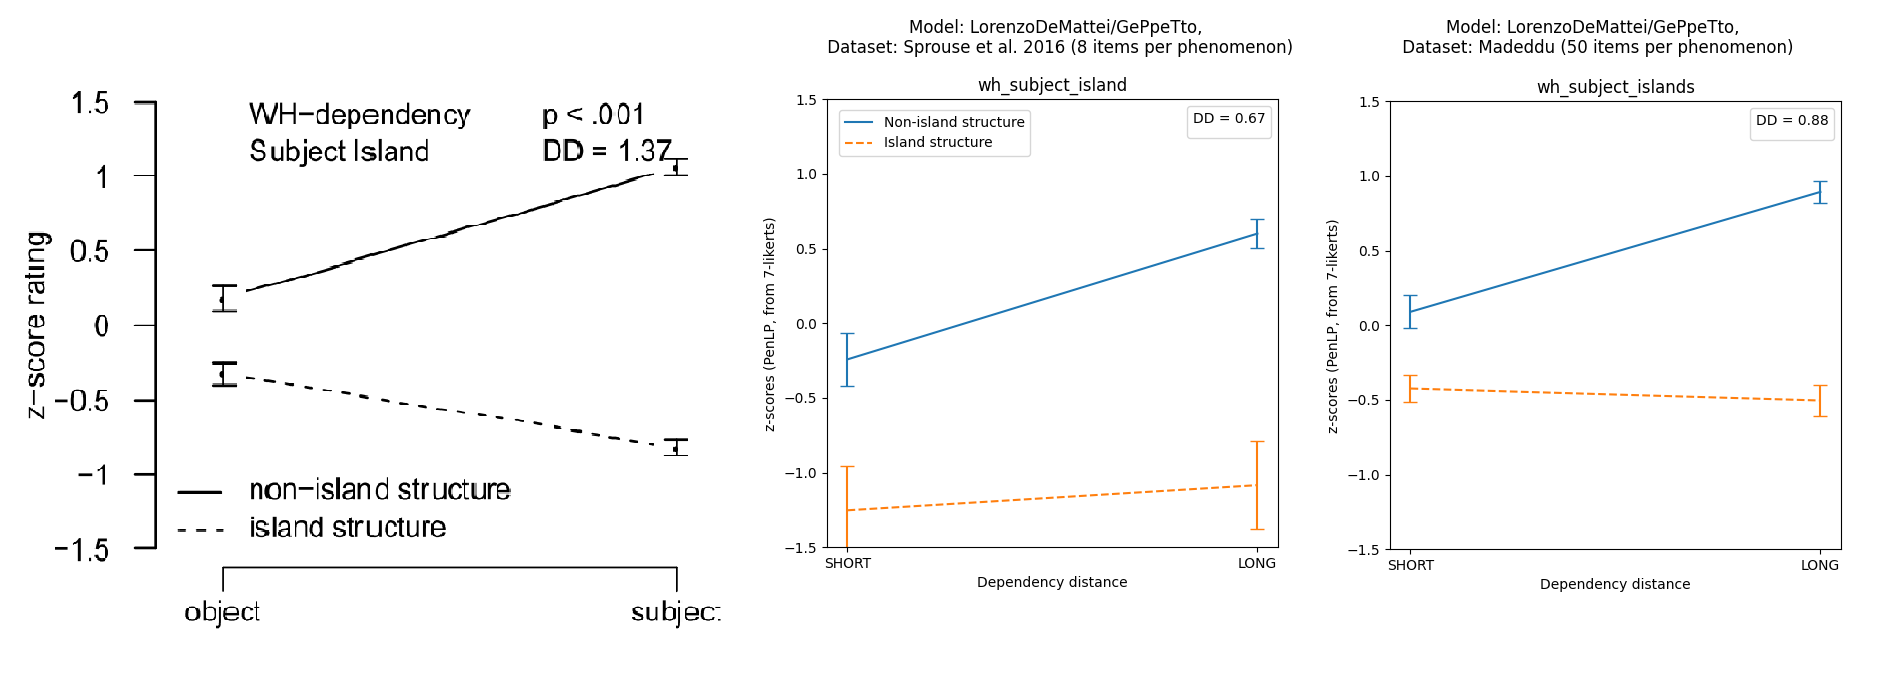
\includegraphics[width=1\textwidth]{images/Chapter1/combined_wh-subject.png} 
%	\caption{Comparison of wh-dependencies subject islands} 
%	\label{fig:wh_subject} % this internally labels the figure for future referencing.
%\end{figure}
%
%In \autoref{fig:wh_subject}, the middle image of Gpt scores on Sprouse data shows significantly lower scores (compared to the human scores on the left image) for the sentences with an island structure (dotted line). % check the sorting of sentences to see why). 
%However, on the right image (Gpt scores on our test suite) they are similar to the human scores. \\
%
%For the non island line, the Short-NonIsland is scored lower then on human subject by Gpt for both testsuites. The Long-NonIsland scores instead are similar  (around 1.0). % but lower on sprouse data. \\
%The slope of the lines on the right image is similar to the one for the human scores (left image). %  oneon the model scores, both for sprouse and new data, but steeper compared to acceptability results on human subjects.

\subsection{Overall considerations}

The plots also reflect the fact, already found by \citet{salazar2020masked}, that for bidirectional models like BERT, it's better not to normalize by sentence lengt the sentence score (the pseudo-log-likelihood), contrary to what proposed by \citet{lau2020furiously}. Comparing the plots for BERT XXL without normalization (\autoref{fig:md_bert_lp}) and with normalization (%\ref{A-fig:md_bert_penlp} 
Figure A.1 in the Appendix)\footnote{In the plots the scoring measures are indicated with the terminology by \citet{lau2020furiously}: LP stands for log probability, which for BERT models it's actually the pseudo-log-likelihood (PLL), while the sentence score normalized with a penalty term based on sentence length is indicated with PenLP.}, we can se that the discrepancies with the human scores are exacertbated when using sentence length normalization. The two lines cross for complex NP islands, they cross even more for subject islands, and are parallel (indicating absence of an island effect) for adjunct islands. Similar divergences from the human plots when using the length-normalized PenLP score also happen with GilBERTo (Figure A.3 in the Appendix vs \autoref{fig:md_gilberto_lp}). 

Conversely, for unidirectional models like GPT-2, the length-based normalization of the sentence score has a beneficial dampening effect to the model score numerical properties, as noted by \citet{salazar2020masked}. And this is also reflected in the plots for GePpeTto, with a divergence from human plots when using the non ideal, unnormalized, LP score (compare \autoref{fig:md_gpt_penlp} with Figure A.4 in the Appendix).



%\subsection{Draft sections}


% next differences to discuss: 
% -take gilberto as the main reference model, since it scores best, best performing model
% -gilberto and subject islands, basically zero difference btween short non island and short island
% -discuss and explain where gilberto scores lower in accuracy (DD based and per sentence type)
% - diff btw tempopral and conditional adjuncts
% -crossing in adjunct islands. Compare examples from conditional adjuncts and from temporal adjuncts
% -discuss other differences in gpt and bert (plots and accuracies)
% note that.. semantic effects are preponderant.. or rather is ..preponderant the fact of having the model designed for a softmax prediciton of a particular words or a few of them. For instance: predicting a common noun, vs a proper name of person, vs a pronoun; ..maybe there is an impact when there a many possibilities in a particular slot (..of a particular word class, or more than one), that would result in a correct sentence.. but the model is geared to the most likely sentence given the context.. so correct words but less likely given the context lower the score of the sentence



% list of confounds to balance / variant sentences to try, scoring and analyzing them with the token surprisals
% -variant for whether islands: use complex wh-word: Quale barca pensi che io abbia affondato? (long non island) so it has the same words (adding "barca") as the short nonisland (Chi pensa che io abbia affondato la barca?)
% -(..whether island) possible more balanced variation: short nonisland = Cosa pensi che io in teoria abbia studiato?
% -subject islands, item 8 gilbert: sostituire luisa a dermatologo, e viceversa
% adjunct island: the main clause premise added to the island sentences, can be added as a previous separate sentence in the nonisland sequences (in this cases each would be composed of two sentences separated by a dot).
% test suite splitting the two adjuncts subtypes. Only keep conditional adjuncts in the main plots, the same as Sprouse
% - replace "avrebbe" in adjuncts non island, balance using the same verb form
% - in adjuncts, replace "il libro" con "il romanzo" and "autore" con "autore di romanzi"

% allegati alla tesi x la controrelatrice:
% excel con test suites
% ? excel con risultati
% ? link al codice nella tesi?
% ? tutti i plots delle surprisals? link a google drive online


% this is due to a lexical and sentence length difference between  .. and the long-nonisland ("\textit{Cosa pensi che io abbia studiato?}"). The short-nonisland sentence contains the phrase "\textit{la teoria}", that is not present in the long-nonisland sentence and causes two spikes in surprisals that make the short-nonisland PLL score (-18.73) worse than the long-nonisland sentence (-14.72). We'll do follow-up experiments balancing the lexical content of the sentences.

% One difference is that for adjunct islands, GPT-2 gives to the \textsc{short-island} sentence gets a higher acceptability score from the transformer model (this might be due to the confound deriving from the format of this sentence, as discussed in section ..).


% For future work we would like to contro for more confounds, splitting the testsuites in smaller ones (of about 20 items each as in Hu et al and ..), each exemplyfying only one paradigm (eg. only conditional ajduncts or only temporal adjuncts), 
% (and controlling for semantic cues, same lexical, using informative/prototypica common nouns instead of proper nouns or pronouns..), having testuites with rarer verbs/nouns ..
% and we would like to compare different approaches to quantify island effects: the one from wilcox, that looks the reduction in gap expectancies, and that of sprouse ..
% see which paradigms are more challeinging
% also different formats of subject, complex np, and wh/whether islands..


%\subsubsection{Complex np islands}



% for future work: automatic generation of examples from templates, like in BLiMP, to control and test more easily for more factors (es. verbs moods and tenses)
% to test for frequency effect: use some rare verb moods/tenses?

% also find an explanation for the other misclassified long non island sentences that use other constructus (with proper agent/patient semantic roles)

% table..

% Mostra una non robustezza del modello nell’apprendimento di strutture sintattiche / or of this use for scoring minimal pairs, non generalizzazione sintattica, in quanto basta una variazione lessicale, anche tra ..parole frequenti, ..per ..alterare ..quale tra due frasi coppie minime sia piu o meno accettabile.
% However, we refer back to section .., about the interpretation/meaning of the Gpt-2 loss ..output/score.


% TODO: table with example items with different constructs, and their scores
% TODO: plots of the whole test suite for this phenomenon with the same variation for all items (using a different verb)


%\subsubsection{Overall observations across all four island phenomena}

% TODO: remaining tables with accuracy scores, comparison with BLiMP extraction islands scores; compare btw models, scoring measures, and datasets (BLiMP, Sprouse, Madeddu)

% todo: all the plots in the appendix (BERT, LP/PenLP, logistic LP/PenLP, .. ) and brief comments 
% (like limitations of BERT acceptability estimates)

% Italian models:
% "LorenzoDeMattei/GePpeTto"
% "dbmdz/bert-base-italian-xxl-cased": ModelTypes.BERT,
% "idb-ita/gilberto-uncased-from-camembert"

% testsuites/datasources:
% Sprouse et al.
% Madeddu

% scoring measures:
% LP/PenLP (softmax-based)
% % LP/PenLP (logistic-based)


%\subsubsection{Discussion on plots from BERT, the logistic function, and PenLP}

% BERT-like models, LP/PenLP scores also based on logistic function scores
% (comment also on the accuracy scores from other models?)

%In \autoref{fig:bert_penlp_l_sprouse} we see the plots of the scores from the BERT model, with the PenLP-L sentence acceptability estimate (using the logistic function rather than the softmax, as described in \autoref{sec:softmax}). Interestingly, it seems that this combination of BERT with the logistic function makes a clear separation between unacceptable sentences (the Long-NonIsland type) and acceptable sentence types, with minimal, if any, difference in score between acceptable sentences.

%\begin{figure}[H]
%	\centering
%	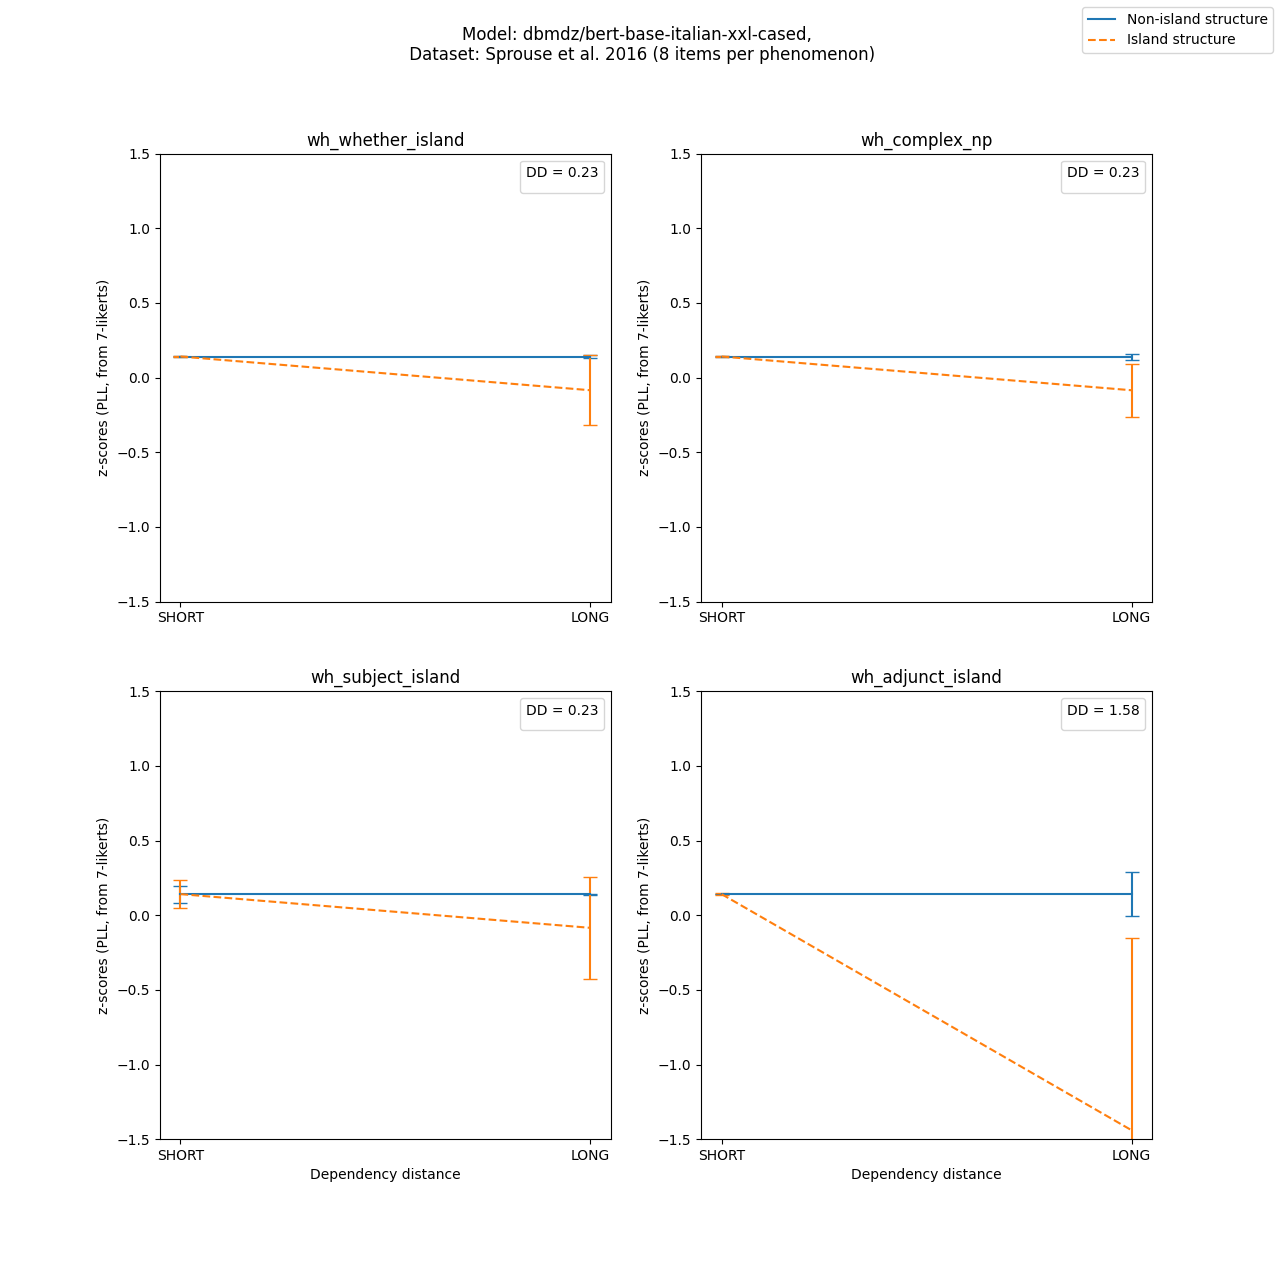
\includegraphics[width=1\textwidth]{images/AppendixA/Sprouse_wh_dbmdz_bert-base-italian-xxl-cased_PLL-zscores-likert-2022-07-11.png} 
%	\caption{Plots from BERT with the PenLP-L sentence acceptability approximation}
%	\label{fig:bert_penlp_l_sprouse}
%\end{figure}

%If we compare these plots with the accuracy scores in \autoref{tab:accuracy_it_data} from this model (BERT, logistic function, PenLP) , we see that they are among the best with an average accuracy of 80.7\%; however, looking at the scores for each phenomenon, the scores are high only in about half the cases, and quite low for the rest: Long-NonIsland sentences of all four island phenomena are scored with 58\%, 64\%, 74\%, 58\% accuracy, and the Short-NonIsland of subject islands with 28\% accuracy.

%TODO: check if this is also a skewing effect of the normalization (from the likert scale and the z-scores) and the presence of much negative large values for the unacceptable sentences: in this case the normalization would ..squeeze together the score for the acceptable sentences, if they have a smaller magnitude.

% With the , the use of the logistic function scores as a basis for LP/PenLP instead results in much ..worse plots (  ). Whether, complex and subject islands get almost identical plots, due to the ..skewing/normalization effect of the discretization and the zscores, because the adjunct islands have much higher magnitude negative values (low acceptability) for the unacceptable sentence (long island.) (? so it seems that with BERT and logistic function scores emerge more clearly a distinction between acceptable and unacceptable sentences, without much differenciation within these two groups).

%\subsubsection{Discussion on plots from GilBERTo}
%
%%Overall, for GilBERTo, the plots are significantly different from those on human ratings. (..)
%
%\begin{figure}[H]
%	\centering
%	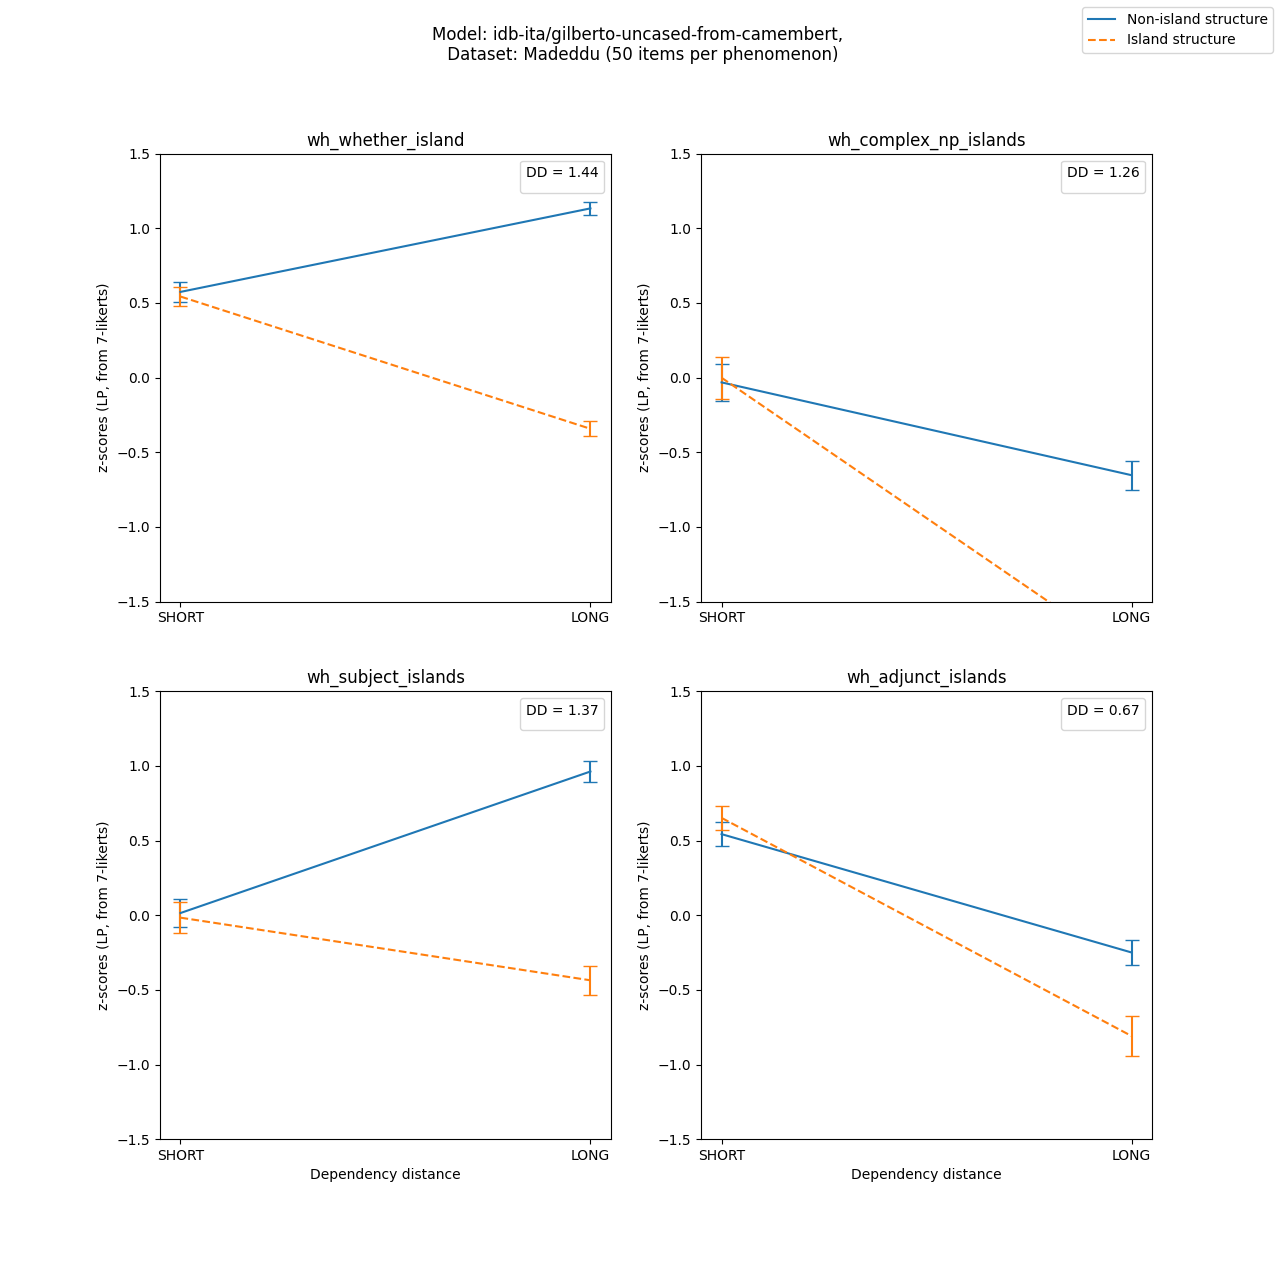
\includegraphics[width=1\textwidth]{images/Chapter1/Madeddu_wh_idb-ita_gilberto-uncased-from-camembert_LP-zscores-likert-2022-09-16_h10m28s27.png} 
%	\caption{Plots from GilBERTo with the LP sentence acceptability approximation}
%	\label{fig:gilberto_lp_madeddu}
%\end{figure}


%\section{Draft notes on the results}
%\subsection{Observation on plots for other models}


%The plots for Geppetto and PenLp are the most similar to the plots on human ratings. However, with the LP measure, the plots differ significantly.
%
%The plots for BERT with PenLP on the Sprouse data are similar to the results on humans from \citet{sprouse2016experimental}, %..with some ..differences..
%
%
%In the plots from the GilBERTo scores, we see that for complex NP and subject islands, the sentences with the island structure receive a higher acceptability than the non island ones (this is no longer the case when removing the penalty for sentence lenght, using the LP sentence acceptability measure). With the PenLP sentence acceptability approximation, the lines tend to have similar slopes, close to being parallel (indicating a lack of, or small, island effect). 

%
%Plots on the Madeddu dataset developed for the present thesis:
%
%BERT, softmax, PenLP and LP
%..
%for adjunct islands, LP seem to work best (without penalizing for sentence lenght).
%Using the logistic function scores, again we see the ..binary differentiation btween unacceptable (long non island) and acceptable (the other 3 types) sentences. However here the plots are more ..flattened, with the scores being very close to the same values.

%We refer to the Appendix for the plots for the other models.

%\subsection{What seems to affect the models acceptability scores}


%\subsubsection{Adjunct islands}
%
%Guardando le short-nonislands, sembra anche qui preponderante il fatto di usare nomi propri di persona (che ha uno score di accettabilità minore) e usare invece di nomi comuni animati/di mestieri/.. (che aumenta l’accettabilità). Ma questo non sembra influenzare il DD score finale % (..evidentemente i vari fattori si bilanciano).
%

%\subsection{Discarded observations on differences between the plots}
%
%\subsubsection{Other notes on  Complex np islands,  what seems to affect the models acceptability scores}
%In \autoref{fig:wh_complex} we see that the non-island line (the line connecting the two acceptability scores for short and long distance dependency sentences without an island structure) is significantly lower in new data (todo: see constructs that increase the score of both long and short)
%
%The (gpt) model seem not to make much difference in ..acceptability btw “regular” subordinates and complex noun phrases ..
%
%-- also the short island point is significantly lower
%
%All the 50 + 8 items of the two test suites (the ones from Sprouse et al and the ones developed for the present thesis), when altered to use the following construct for the complex NP "avuto l'intuizione che" (had the intuition that), are scored by the model as if there is no island restriction violation anymore. 
%
%il verbo “intuire” diminuisce ..l’accuratezza del giudizio di accettabilità
%in particolare diminuzione della accettabilità delle frasi long nonisland (con long distance wh dependency e struttura non island), che ricevono accettabilità minore di quelle con struttura island:
%Esempio analisi variazioni con verbo “intuire” complex np, ..
%
%the verb form “sapeva” (imperfect), compared to ..present perfect forms (“ha osservato/affermato/..”) seems to get better DD score in complex np islands (and also in another phenomenon ..).
%
%\subsubsection{Whether islands}
%NB: note that according to human scores, for this type of whether island sentences, the "correct" scoring is to have an increase in acceptability going from short to long non island sentences.
%Maybe comparing the scores between acceptable sentences (in this case short and long non islands), expecting it to match humans acceptability judgements .. is beside the present ..research question.
%In any case, we noted a reverse in the acceptability difference between this two types of sentences (short and long non islands) when changing the subject of the subordinate sentence from a personal pronoun ("io", 1st pers sg), to a proper noun (i.e. "Gianni"), to a common noun (i.e. "il parlamentare").

%-- significant variation in acceptability diff between short non island and long non island, when replacing: the personal pronouns io/lei, with a proper noun like "Gianni", or even more with a noun like "il parlamentare" (the congressman). In this latter case, significant improvement toward the expected acceptability rate (only 10 out of 50 are .."missclassified"). With the proper noun "Gianni", 18 are missclassified. With the personal pronoun 29 out of 50 are missclassified.
%Try replacing with .. another proper noun, more common like ..
%
%
%(tables and examples of these variations to put on the thesis/report?)
%
%(possible explanation: personal pronouns and proper nouns might be less common in the type/genre of corpora these models were trained on, like wikipedia).
%Observations: the direct objects in the examples are all relatively common words..\footnote{\citet{wei2021frequency} found significant frequency effects (but for agreement .. tests, which are much easier to isolate), for items that occurr rarely in the training corpus (..less then ..10-100 times). But to notice this effect they had to purposly tweak the training corpus. Replicating this for a preexisting corpus (using very rare vocabulary ..) is much more complex and out of the scope of the present study.}
%try with rarer ones.
%..
%-- both on sprouse and new data, gpt "incorrectly" increases the accceptability from short to long non island (check constructs that instead decrease the acceptability?)


%\section{BLiMP English dataset}
%
%\subsection{English models details}
%
%
%\section{Token surprisal analysis}


%We found the most informative analysis (rather than the factorial test design) was looking at the token surprisals for the Bert-like models (do it also on the Gpt2 logits?).
%..
%(even more informative, or complementary, would be to look at the activations in the model layers)
%
%
%
%"The ratio of token-level PPPLs between unacceptable and
%acceptable sentences overall increases with performance, separating the two sentence sets" \citep{salazar2020masked}
% plot token surprisal on Blimp sentences, compare spikes of minimal pairs differing for just one word


%\section{Follow up experiments}
%
%\subsection{Variations on Complex NP islands, scores from GPT-2}

% complex NP plots, GPT-2
%Doing some variations experiments (see  \autoref{tab:compare1}), we found that by replacing the main clause verbs with "intuire che"/"avere l'intuizione che" ("to sense that" / "to have the intuition that") or "avvertire che"/"avere il sentore che" ("to feel that" / "to have an inkling that") or "percepire che"/"avere la percezione che" ("feel that"/"to have the feeling that"), the island restriction violation seem to have no effect, and the Long-Island sentence becomes more acceptable than the same sentence without the island structure (Long-NonIsland).
%
%Indeed, the sentence \textit{Cosa hai avuto l'intuizione che il portavoce avrebbe confermato?} (\textit{`What did you have the intuition that the spokeperson had confirmed?'}), seems acceptable despite extracting from a complex NP construct. 
%
%An hypothesis, whose demonstration we leave for future work, is that this is due to main clause expressions in which the subject has the semantic role of an \textsc{experiencer} rather than an \textsc{agent}, which could be a condition for Complex NP island restrictions to enter into effect or not. 
% "avrebbe ppt" (condizionale passato)
% In fact, it seems that the Gpt-2 model correctly captures the fact that with these constructs the long nonisland sentences become acceptable.

%\begin{table} \scriptsize 
%	\begin{center}
%		\begin{tabular}
%			{p{0.3\linewidth} p{0.08\linewidth} p{0.3\linewidth} p{0.08\linewidth} p{0.08\linewidth}|} \\
%			\multicolumn{2}{c}{\textbf{\textsc{Long-NonIsland}}} & \multicolumn{2}{c}{\textbf{\textsc{Long-Island}}}  &   \\
%			\textbf{text} & \textbf{PenLP} & \textbf{text} & \textbf{PenLP} &  \textbf{Diff}  \\
%			\hline
%			\textit{Cosa hai messo in dubbio che il portavoce avrebbe confermato?} & -31.65
%			& \textit{Cosa hai messo in dubbio la previsione che il portavoce avrebbe confermato} & -33.21 & 1.56 \\ 
%			\textit{Cosa hai intuito che il portavoce avrebbe confermato?} & -32.36 
%			& \textit{Cosa hai avuto l'intuizione che il portavoce avrebbe confermato?} & -29.99 & -2.37 \\ 	
%			% TODO: use the other verbs too:  "avvertire che"/"avere il sentore che" ,  "percepire che"/"avere la percezione che" 
%			\textit{Cosa hai detto che Gianni avrebbe sollevato?} & -33.74 
%			& \textit{Cosa hai riferito il fatto che Gianni avrebbe sollevato?} & -36.64 & 2.90 \\ 
%			\textit{Cosa hai intuito che Gianni avrebbe sollevato?} & -34.31 
%			& \textit{Cosa hai avuto l'intuizione che Gianni avrebbe sollevato?} & -30.52  & -3.79 \\ 
%			
%			\textit{Cosa hai messo in dubbio che io avrei vinto?} & -26.48 & 
%			\textit{Cosa hai messo in dubbio la previsione che io avrei vinto?} & -30.17 & 3.69\\ 				
%			\textit{Cosa hai intuito che che io avrei vinto?} & -29.49 & 
%			\textit{Cosa hai avuto l'intuizione che io avrei vinto?} & -24.45  & -5.04 \\ 				
%			
%		\end{tabular}
%		\caption{Comparing acceptability variations among sentences in the complex NP dataset. A positive difference indicates that the Long-NonIsland sentence is more acceptable than the Long-NonIsland one, as expected.}
%		\label{tab:compare1}
%	\end{center}
%\end{table}


%\bigskip
%% TODO: insert plot of variations
%With other variations experiments, we found that replacing the main clause verb with "sapeva che"/"conosceva che" ("he knew that", see examples in table ..TODO), increases the acceptability of the long-non island sentences; on the other hand, this variation results in a lower acceptability to the short island sentence, compared to the scores from human subjects, and by this way the non-island and island line end up being almost parallel, with the DD score close to zero (which indicates an almost absent island effect).
%\\ 
%TODO: add table and plots of senteces with  "sapeva che"/"conosceva che" 

% todo: show tables with examples "sapeva che" % todo: numbered examples like formulas
% todo: show the plots for "intuizione che", "sapeva che" (two subfigures, each numbered/lettered to be referenced)

% examples of complex np items before and after the "avuto l'intuizione che" variation: ..
% show the plots for the items using this construct ("avuto l'intuizione che" ), it seems strange scores are given
% (the island line is higher than the non island one, but they are all acceptable sentence and there is no island restriction anymore)

%\subsection{Variations on whether islands}
%Experimenting with other sentence variations for whether islands, we found that a variation that aligns the plots more to those from the humans' scores, is replacing the personal pronouns (like "io") with proper nouns (like "Gianni") or common nouns (like “il parlamentare”, or “lo studente”)  like in this example: 
%
%\begin{example}	\textsc{Whether islands, Long-Island sentence type}
%	\renewcommand{\labelenumi}{\alph{enumi}.}
%	\begin{enumerate}
%		\item 
%		Cosa ti domandi se io abbia riscosso?
%		\item 
%		Cosa ti domandi se Gianni abbia riscosso?
%		\item 
%		Cosa ti domandi se il parlamentare abbia riscosso?
%	\end{enumerate}
%	\label{variation_2}
%\end{example}

% This might be the reason for the discrepancies in some of the 4 phenomena: some make more use of ..nomen agentis, while others rely more on personal pronuns. Try this replacement this in all 4 test sets.
%TODO: put scores values and/or to quantify the effect of these variations.

%TODO: test sentence variations using less common verb tenses and moods (but consistently across an item or even all items of a suite)
% Not much difference seems to derive by using less common (..) verbs
% (examples in which both sentences in a pair also specify the direct object, see how this affects the score? Like long nonisland vs long island ..)


%\subsection{Other follow up experiments}

% finetune the models for acceptability? (already existin italian models for this, like from Trotta et al. 2021?)
% finetuning is very fast anyway 
% (fine tune also for english the Bostrom models?)

% (also to the plot on acceptability score by sentence lenght?)

% what about a follow up analysis on the thesis, based on the results? like manipulating data to check the effect of somee factors, ..


%Analizzare le attivazioni nei vari livelli del modello ..
%Fare un training .”a strati”, in cui in ciascuno strato c’è il target dell’apprendimento di un livello di base della lingua (morfologia, sintassi, semantica, ampiezza del vocabolario, ..), con strati successivi che aumentano la complessità della conoscenza che il modello ha del linguaggio.
%
%
%Confronto percentuali accuratezza (short/long non island, short island) con quelle in BLiMP
%(and other works with extraction islands evaluations?)

% test the worst scoring examples (incorrect, and with the highest PLL diff btw acceptable/unacceptable sentences)
% test balancing island sentences, addint rare words to the long island (eg. "mediatore")
% test changing the ..minimal pairs/sentences in a item like Wilcox rather than Sprouse. Staring from the long island, remove the dependency (instead of making it short, which changes the lexical content)

% in the intro section to island effects, explaining what they are, also say that repeated exposure increases their acceptability (..so maybe it's just their rarity that makes them unacceptable.. language is use.. if they where more common, because needed for some comunicative goals, they would become acceptable..) (maybe this is true, or more the case, for some island types than others)

% confound: try with items that gives semantic cues (the single omitted word is very likely given the verb before and the ..modifier after it, and sentences that don't give such cues, like more vague verbs and modifiers, or no modifiers; generic modifiers: time specifiers)

% complex np are already balanced
% wh could be better balanced
% subject islands are the trickiest to balance ..
% adjuncts ..

% todo: chiarire i vari tipi di subject islands ..
% compare the subject islands definition (and the other types) by Wilcox and by Sprouse

% Wilcox: "The Complex NP Constraint (CNPC) holds that a gap cannot be hosted in a sentential clause dominated by a noun phrase with a lexical head noun. This constraint accounts for the unacceptability of (8b), (8c), (8f) and (8g) below. The CNPC does not apply to other NP modifiers, such as PPs, unless the modified NP occurs in subject position (Huang, 1982). This ban, called the Subject Constraint (SC), accounts for the unacceptability of (8h) compared to (8d)."

% "Subject islands " "as movement out of the subject NP " \citep{sprouse2013experimental}
% IP: inflectional phrase (IP) 
% CP: complementizer Phrase

% do all movements from the subject NP result in island violation effects?

italian rc-dependencies, in the case of, introduced only by ..oblique relative pronouns
"one global decision that we made was to investigate rc-dependencies that form restrictive relative clauses introduced by a relative pronoun (as opposed to appositive relatives or restrictive relatives introduced by a complementizer, which we leave to future research). This had two major consequences. First, all of the rc-dependencies in Italian had to be constructed with oblique (PP) argument gaps" 
("con il/dal quale/su/da/con cui, " etc.)
"because Italian restrictive relatives can only be introduced by a relative pronoun when the head of the relative is an oblique argument (subjects and direct objects can only be introduced by the complementizer che ‘that’). This led to a systematic difference between Italian rc-dependencies, which were constructed with oblique argument gaps, and English rc-dependencies, which were constructed with direct object gaps."

% restrictive relative clauses introduced by a relative pronoun
% as opposed to appositive relatives 
% or restrictive relatives introduced by a complementizer



% recap the cross lingual diffs in En and It about island effects
% then edit/write the whole chapter
% add notes to other chapters in the analysis of results, formation of the dataset, ..


% (future work: more challenging tests, controlling for frequency effects/more marginal web forms: do the accuracy/island effects captured by the model ..degrade when less common constructs/verb forms are used?)

\section{Follow up experiments and future work}

In future work, we plan to do some follow-up experiments ..
% We want to analyze the plots for GPT-2 per token surpisal as done for the other models\footnote{This will require some more coding that is out of the time constraints for this thesis.}, to explain more clearly and in more detail the outcome of the performance scores. In particular, we want to investigate wy GPT-2 scored so low (46\% accuracy) for complex NP islands. Obtaining the 


\chapter{Conclusions}
% mention in the conclusions/discussions about the confounds due to semantic full words that produce spikes .. that the softamax function, and the fact that these models are trained to learn a probability distribution of language.. goes contrary to the actual use of language that "does not maximize probability" (cite ref)

In assessing transformer-based  language models, trained in the Italian language, on syntactic phenomena known as island effects, we found that the models responses for some types of island effects can mirror or resemble that of humans, as observed in previous psycholinguistic studies.

We found that the factorial experimental design we adopted from psycholinguistic studies was able to implicitly control for some unexpected confounds, when they were evenly distributed within the test items. However, as it is the case with assessment approaches based on minimal pairs, also in a factorial experimental setup sentences within an item should have ideally exactly the same lexical content, in order to avoid confounds. This is a challenging tasks in the development of tests covering more complex syntactic phenomena like island effects.

Our results confirm previous work that indicates that to master more complex syntactic phenomena, like island effects, modern transformer-based language models still require an amount of training data above the threshold of 100M tokens, which is the amount of data to which humans are exposed when they learn language, and also the threshold at which transformer-based models have been shown (although possibly by test suites not challenging enough) to acquire knowledge of most (but not all) syntactic and semantic phenomena.

In our contribution to the relatively novel line of research of the targeted syntactic evaluation of deep neural language models, an area for which adequate methodologies are sill in development, we found that it is an effective and informative approach to complement the performance scores achieved by the models, with the qualitative analysis of per-token surprisals, which reveal to which phenomena a model shows sensitivity. This combination of approaches seems also a promising avenue to reach better models explainability.

We agree with previous work \citep{wilcox2018rnn, ettinger2020bert} that observed that developing more comprehensive and more challenging targeted linguistic tests for modern language model can play a significant role in accelerating their development. 

% TODO? also discuss, with examples, the choices made in BLiMP to test the same phenomena (in blimp: confound because of wrong ..word sequences?)

% there seems to be errors in the sentences generated by Wilcox et al. for wh-rc/subj: "The newspaper reported that the novel who the famous author received favorable reviews in the press . <eos>"

%\chapter{Note sections to remove}
%\section{misc ideas with notes}

%(misc ideas with notes)
%using multiple POS taggers and semantic role taggers etc.
%one, the default, for most common (..more prototypical) sentences/structures
%the other ones, used in ..garden path scenarios, when multiple indicators show that some POS tags or semantic role or other category might be wrong.
%the second set of taggers should do a ..full parsing analysis.. combining and ranking different parsing hypotheses)
%
%
%(on perplexity: the target of "low perplexity" in a language model, should not be in the ..words themselves, because language has informative/comunicative goals that are to introduce new, less predictable, information; it should be at other levels, like that of correctedness/acceptability; target of low perplexity of POS tags, semantic role tags, etc.) \\
%\citet{von2018pos} use perplexity on POS tags as a measure of syntactic complexity;
%"working on POS sequences avoids having to deal with data sparsity issues." \citep{von2018pos}
%
%what about using perplexity on POS tags as a measure/estimation of syntactic well formedness?
%": Lawrence et al. (2000) train RNNs to do
%acceptability classification over sequences of POS
%tags corresponding to example sentences from a
%syntax textbook."
%
%discriminate btw complex/rare vs unacceptable? a threshold (linearly separable) on perplexity? Or multiple dimensions, non linearly, should be used?
%(but if there is a wrong/mispelled word.. the pos tagger might misclassify it)
%(distinguishing ..sentence unacceptability by linguistic level: morphological mistakes/typos, ..word order errors, ..)
%(also: perplexity uses a markov model of language? no, but multiplication the perplexity of each word to obtain the perplexity of the whole sequence.. a "less linear" formula might be needed..)
%(montemagni et al paper on profileU on linguistic profiling? use for sentence acceptability estimates? use for ..style detection/automated analysis ..


%\section{Misc notes with refs}


%First work with targeted syntactic tests on modern language models (RNNs or transformers) is \citet{linzen2016assessing}, while first use of psycholinguistic tests for modern LM is from \citet{futrell2018rnns}.
%
%“NATURAL LANGUAGE DOES NOT MAXIMIZE PROBABILITY” 
%“Why is human-written text not the most probable text? We conjecture that this is an intrinsic property of human language. Language models that assign probabilities one word at a time without a global model of the text will have trouble capturing this effect. Grice’s Maxims of Communication (Grice, 1975) show that people optimize against stating the obvious. Thus, making every word as predictable as possible will be disfavored. This makes solving the problem simply by training larger models or improving neural architectures using standard per-word learning objectives unlikely: such models are forced to favor the lowest common denominator, rather than informative language.” 
%\citep{holtzman2019curious}
%
%
%
%
%
%"Auxiliary training objectives Adding auxiliary unsupervised training objectives is an alternative form of semi-supervised learning. Early work by Collobert and Weston [10] used a wide variety of auxiliary NLP tasks such as POS tagging, chunking, named entity recognition, and language modeling to improve semantic role labeling. More recently, Rei [50] added an auxiliary language modeling objective to their target task objective and demonstrated performance gains on sequence labeling tasks. Our experiments also use an auxiliary objective, but as we show, unsupervised pre-training already learns several linguistic aspects relevant to target tasks." (Radford Gpt)
%
%survey on alternative training tasks etc.: paper "a primer on BERTology"
%
%"QUALITATIVE ANALYSIS" (REASONING ABOUT ENTAILMENT WITH NEURAL ATTENTION, Tim Rocktaschel et al. 2016)
%
%"Efficiency considerations are important when building language models that use
%such large sets of n-grams. Rather than store each word as a string, it is generally
%represented in memory as a 64-bit hash number, with the words themselves stored
%on disk. Probabilities are generally quantized using only 4-8 bits (instead of 8-byte floats), and n-grams are stored in reverse tries." (Jurafsky 2021 3rd ef ch.3)
%
%"the standard information theory textbook Cover and Thomas (1991). "
%
%"It uses the output of a character-level
%Convolutional Neural Network (CNN) as input to
%the LSTM. This model has the best published perplexity for English text." \citep{wilcox2018rnn}
%
%"We also replaced numbers (exponential, comma separated etc) with a <NUM> tag."    \citep{chowdhury2018rnn}

% "A qualitative inspection suggests that the low accuracy in the verb conjunction case (67.5%) is due to ambiguous sentences such as “if you have have have have any have questions or need need need need/ need needs needs needs needs”, where the target can be needs re-interpreted as a noun that is acceptable in the relevant context.9" "These results are in line with human experimental studies that found that richer morphology correlates with fewer agreement attraction errors (Lorimor et al., 2008). " Gulordava et al 2018

% Tests on nonce words, and similar: "As a proof of concept, Pereira (2000) and, later, Mikolov (2012) computed the probability of Chomsky’s famous “colorless green ideas” sentence using a class-based bigram LM and an RNN, respectively, and showed that it is much higher than the probability of its shuffled ungrammatical variants." Gulordava et al 2018

% quoting in the thesis: "However, Tenney et al. (2019a) remark, ‘‘the fact that a linguistic pattern is not observed by our probing classifier does not guarantee that it is not there, and the observation of a pattern does not tell us how it is used.’’ There is also the issue of how complex a probe should be allowed to be (Liu et al., 2019a)."  \citep{rogers2020primer}

% "Another direction is information-theoretic probing. Pimentel et al. (2020) operationalize probing as estimating mutual information between the learned representation and a given linguistic property, which highlights that the focus should be not on the amount of information contained in a representation, but rather on how easily it can be extracted from it. Voita and Titov (2020) quantify the amount of effort needed to extract information from a given representation as minimum description length needed to communicate both the probe size and the amount of data required for it to do well on a task" \citep{rogers2020primer}.

%\section{Notes and refs on incorporating explicit semantic info}

% "Syntax in LMs: There have been several proposals over the years to incorporate explicit syntax into LMs" ", in practice it can still be beneficial to inject syntax into the model. This can be done by combining it with a supervised parser (Dyer et al., 2016) or other multi-task learning objectives (Enguehard et al., 2017)" \citep{marvin2018targeted}

% "Multi-task training with a syntactic objective (CCG supertagging) mitigated this drop in performance for some but not all of the dependencies we tested. We conjecture that the benefits of the inductive bias conferred by multi-task learning will be amplified when the amount of training data is limited"  \citep{marvin2018targeted}
% (that is, incorporating linguitic signals could be effective in lowering the amount of training data needed)

% "Second, we find a larger effect of model inductive bias than training data size on SG score, a result that accords with van Schijndel et al. (2019). Models afforded explicit structural supervision during training outperform other models: One structurally supervised model is able to achieve the same SG scores as a purely sequence-based model trained on ∼100 times the number of tokens. Furthermore, several Transformer models achieve the same SG score as a Transformer trained on ∼200 times the amount of data. " \citep{hu2020systematic}

% Alternative training tasks:
% "Task reformulation: Language model is usually pre-trained with a Masked Language Modeling (MLM) objective, which is motivated by Cloze task in (Taylor, 1953). There have been several works reformulating few-shot learning tasks as cloze questions to reuse pre-trained LM such as LM prompt (Jiang et al., 2020), PET (Radford et al., 2019; Schick \& Schutze, 2020a), and recent ¨ LM-BFF (Gao et al., 2020). It shows a pre-trained LM can achieve non-trivial performance with few annotated samples. There are also some other works transforming NLP tasks as generative QA tasks (Puri \& Catanzaro, 2019)." but low performance on CoLA (possible beacuse of "different data distribution"): "The only exception is the CoLA (the linguistic acceptability task). It is might due to that MLM pre-trainng and entailment training did not see this type of data distribution before"

% enriched training data (with supervised tasks): "Intermediate training: The work by (Phang et al., 2018) shows that supplementing pre-trained LMs with further training on data-rich supervised tasks can obtain additional performance improvements on the GLUE benchmark."

% Freezing / Frozen Layers:
% "The results align with Lee et al. (2019), who discuss the performance degradation of BERT-based models depending upon the number of frozen layers." (Cherniavskii et al. 2022)

% BAAYEN, R. HARALD. 2007. Analyzing linguistic data: A practical introduction to statistics using R. Cambridge: Cambridge University Press.
% BAAYEN, R. HARALD; DOUGLAS J. DAVIDSON; and DOUGLAS M. BATES. 2008. Mixed-effects modeling with crossed random effects for subjects and items. Journal of Memory and Language 59.390–412.

% "Other studies have investigate how one model’s linguistic  knowledge changes during the training process, as a function of the number of updates (Saphra and Lopez, 2019; Chiang et al., 2020)." (Raffel et al 2020, T5 paper)

% works that tracks the progress in performance on linguistic tests during training (cited in paper by ..)(T5? Venturi? Zhang when do you need ..?)

% "The method we use in this work, which is currently common practice, is to train the model to denoise corrupted spans of text. We suspect that this simplistic technique may not be a very efficient way to teach the model general-purpose knowledge. More concretely, it would be useful to be able to attain good fine-tuning performance without needing to train our models on 1 trillion tokens of text first. Some concurrent work along these lines improves efficiency by pre-training a model to distinguish between real and machine-generated text (Clark et al., 2020)." (Raffel et al 2020, T5 paper)

% notes: as reported in previous papers (..), some tests that are completed to human level by SoTA models might not be challenging enough. ..probably the claim that syntax and semantics are learnet with 100M tokens should be read : most syntax andd semantics.. but not more challenging phenomena. But we need more challenging tests, were, for the same tests, there are equivalent with new/rarer words (one/few shot tests), to check that the genaralizations are robust. This is separate from the problema that some more advanced semantic and maybe syntactic tests need pragmatic/commonsense knowledge and that's why they are failed. Review paper "quantity doesn't buy quality"

% nonetheless, even in the T5 (Raffel et al. 2020), it says that these models shouldn't need 1T data to ace ..common sense benchmarks.
% multimodal / multitask training settings to be more comparable to the learning setting of humans. Images, sounds (prosody/.. signals), .. Automatically generate the training sets for these. Part of these might be useful for any language.. the images. Although the images also are rapresentative of a particular culture. Sound that are not linguistic sounds, like noises, can be used as grounding for any language.


% alternative training strategies, tasks, linguistic supervision, augmentation, .. "This approach can be extended to the training stage: neural networks can be encouraged to develop more sophisticated generalizations by oversampling grammatically challenging training sentences. "  ". This training regime indeed improved the performance of the network; however, the improvement was quantitative rather than qualitative: there was limited generalization to dependencies that were even more difficult than those encountered in training. Further experiments are needed to establish the efficacy of this method." \citep{linzen2016assessing}

% benefits from targeted linguistic training: "A network that has acquired syntactic representations sophisticated enough to handle subject-verb agreement is likely to show improved performance on other structure-sensitive dependencies, including pronoun coreference, quantifier scope and negative polarity items." 
% "As such, neural models used in NLP applications may benefit from grammatically sophisticated sentence representations developed in a multitask learning setup (Caruana, 1998), where the model is trained concurrently on the task of interest and on one of the tasks we proposed in this paper." " Of course, grammatical phenomena differ from each other in many ways. The distribution of negative polarity items is highly sensitive to semantic factors (Giannakidou, 2011)." island effects / constraints: "Restrictions on unbounded dependencies (Ross, 1967) may require richer syntactic representations than those required for subject-verb dependencies" \citep{linzen2016assessing}

% "This could mean that either BERT’s syntactic knowledge is incomplete, or it does not need to rely on it for solving its tasks. The latter seems more likely, since Glavasˇ and Vulic (2020) report that an intermediate ´ fine-tuning step with supervised parsing does not make much difference for downstream task performance" \citep{rogers2020primer}

% "Out-of-the-box BERT is surprisingly brittle to named entity replacements: For example, replacing names in the coreference task changes 85% of predictions (Balasubramanian et al., 2020). This suggests that the model does not actually form a generic idea of named entities, although its F1 scores on NER probing tasks are high (Tenney et al., 2019a). Broscheit (2019) finds that fine-tuning BERT on Wikipedia entity linking ‘‘teaches’’ it additional entity knowledge, which would suggest that it did not absorb all the relevant entity information during pre-training on Wikipedia" \citep{rogers2020primer}

% "BERT struggles with pragmatic inference and role-based event knowledge (Ettinger, 2019). BERT also struggles with abstract attributes of objects, as well as visual and perceptual properties that are likely to be assumed rather than mentioned (Da and Kasai, 2019)"  \citep{rogers2020primer}

% " In order to retrieve BERT’s knowledge, we need good template sentences, and there is work on their automatic extraction and augmentation (Bouraoui et al., 2019; Jiang et al., 2019b)." "The MLM component of BERT is easy to adapt for knowledge induction by filling in the blanks (e.g., ‘‘Cats like to chase [ ]’’)."  \citep{rogers2020primer}

% "However, BERT cannot reason based on its world knowledge. Forbes et al. (2019) show that BERT can ‘‘guess’’ the affordances and properties of many objects, but cannot reason about the relationship between properties and affordances. For example, it ‘‘knows’’ that people can walk into houses, and that houses are big, but it cannot infer that houses are bigger than people" \citep{rogers2020primer}

% "The first layer of BERT receives as input a combination of token, segment, and positional embeddings. It stands to reason that the lower layers have the most information about linear word order. Lin et al. (2019) report a decrease in the knowledge of linear word order around layer 4 in BERT-base. This is accompanied by an increased knowledge of hierarchical sentence structure, as detected by the probing tasks of predicting the token index, the main auxiliary verb and the sentence subject." "4These BERT results are also compatible with findings by Vig and Belinkov (2019), who report the highest attention to tokens in dependency relations in the middle layers of GPT-2." \citep{rogers2020primer}

% "There is conflicting evidence about syntactic chunks. Tenney et al. (2019a) conclude that ‘‘the basic syntactic information appears earlier in the network while high-level semantic features appear at the higher layers’’, drawing parallels between this order and the order of components in a typical NLP pipeline—from POS-tagging to dependency parsing to semantic role labeling. Jawahar et al. (2019) also report that the lower layers were more useful for chunking, while middle layers were more useful for parsing. At the same time, the probing experiments by Liu et al. (2019a) find the opposite: Both POS-tagging and chunking were performed best at the middle layers, in both BERT-base and BERT-large. However, all three studies use different suites of probing tasks." \citep{rogers2020primer}

% "Tenney et al. (2019a) suggest that whereas syntactic information appears early in the model and can be localized, semantics is spread across the entire model, which explains why certain non-trivial examples get solved incorrectly at first but correctly at the later layers. This is rather to be expected: Semantics permeates all language, and linguists debate whether meaningless structures can exist at all (Goldberg, 2006, p.166–182). But this raises the question of what stacking more Transformer layers in BERT actually achieves in terms of the spread of semantic knowledge, and whether that is beneficial. Tenney et al. compared BERT-base and BERT-large, and found that the overall pattern of cumulative score gains is the same, only more spread out in the larger model." \citep{rogers2020primer}

% "• What to mask. Masks can be applied to full words instead of word-pieces (Devlin et al., 2019; Cui et al., 2019). Similarly, we can mask spans rather than single tokens (Joshi et al., 2020), predicting how many are missing (Lewis et al., 2019). Masking phrases and named entities (Sun et al., 2019b) improves representation of structured knowledge."  \citep{rogers2020primer}

% "The prominence of syntactic information in the middle BERT layers is related to Liu et al.’s (2019a) observation that the middle layers of Transformers are best-performing overall and the most transferable across tasks (see Figure 4)."  \citep{rogers2020primer}

% "There is a wide consensus in studies with different tasks, datasets, and methodologies that syntactic information is most prominent in the middle layers of BERT.4"  \citep{rogers2020primer}

% "Human language is incredibly complex, and would perhaps take many more parameters to describe fully, but the current models do not make good use of the parameters they already have. Voita et al. (2019b) showed that all but a few Transformer heads could be pruned without significant losses in performance. For BERT, Clark et al. (2019) observe that most heads in the same layer show similar self-attention patterns (perhaps related to the fact that the output of all self-attention heads in a layer is passed through the same MLP), which explains why Michel et al. (2019) were able to reduce most layers to a single head."  \citep{rogers2020primer}

% "we list what we believe to be the most promising directions for further research. Benchmarks that require verbal reasoning." \citep{rogers2020primer}% "Although BERT enabled breakthroughs on many NLP benchmarks, a growing list of analysis papers are showing that its language skills are not as impressive as they seem. In particular, they were shown to rely on shallow heuristics in natural language inference (McCoy et al., 2019b; Zellers et al., 2019; Jin et al., 2020), reading comprehension (Si et al., 2019; Rogers et al., 2020; Sugawara et al., 2020; Yogatama et al., 2019), argument reasoning comprehension (Niven and Kao, 2019), and text classification (Jin et al., 2020). Such heuristics can even be used to reconstruct a non–publicly available model (Krishna et al., 2020). As with any optimization method, if there is a shortcut in the data, we have no reason to expect BERT to not learn it. But harder datasets that cannot be resolved with shallow heuristics are unlikely to emerge if their development is not asvalued as modeling work"  \citep{rogers2020primer}
% NB: bias for modeling work rather than ..less technical but bigger picture approaches/directions..

% "Developing methods to ‘‘teach’’ reasoning. While large pre-trained models have a lot of knowledge, they often fail if any reasoning needs to be performed on top of the facts they possess (Talmor et al., 2019, see also subsection 3.3). For instance, Richardson et al. (2020) propose a method to ‘‘teach’’ BERT quantification, conditionals, comparatives, and Boolean coordination."   \citep{rogers2020primer}

% "Learning what happens at inference time. Most BERT analysis papers focus on different probes of the model, with the goal to find what the language model ‘‘knows’’. However, probing studies have limitations (subsection 3.4), and to this point, far fewer papers have focused on discovering what knowledge actually gets used. Several promising directions are the ‘‘amnesic probing’’ (Elazar et al., 2020), identifying features important for prediction for a given task (Arkhangelskaia and Dutta, 2019), and pruning the model to remove the non-important components (Voita et al., 2019b; Michel et al., 2019; Prasanna et al., 2020)."  \citep{rogers2020primer}

% \nocite{lau2020furiously, bostrom2020byte, futrell-etal-2019-neural}
